\documentclass[10pt,a4paper]{article}
\usepackage[UTF8,fontset = windows]{ctex}
\setCJKmainfont[BoldFont=黑体,ItalicFont=楷体]{华文中宋}
\usepackage{amssymb,amsmath,amsfonts,amsthm,mathrsfs,dsfont,graphicx}
\usepackage{ifthen,indentfirst,enumerate,color,titletoc}
\usepackage{tikz}
\usepackage{multicol}
\usepackage{makecell}
\usepackage{longtable}
\usetikzlibrary{arrows,calc,intersections,patterns,decorations.pathreplacing,3d,angles,quotes,positioning}
\usepackage[bf,small,indentafter,pagestyles]{titlesec}
\usepackage[top=1in, bottom=1in,left=0.8in,right=0.8in]{geometry}
\renewcommand{\baselinestretch}{1.65}
\newtheorem{defi}{定义~}
\newtheorem{eg}{例~}
\newtheorem{ex}{~}
\newtheorem{rem}{注~}
\newtheorem{thm}{定理~}
\newtheorem{coro}{推论~}
\newtheorem{axiom}{公理~}
\newtheorem{prop}{性质~}
\newcommand{\blank}[1]{\underline{\hbox to #1pt{}}}
\newcommand{\bracket}[1]{(\hbox to #1pt{})}
\newcommand{\onech}[4]{\par\begin{tabular}{p{.9\textwidth}}
A.~#1\\
B.~#2\\
C.~#3\\
D.~#4
\end{tabular}}
\newcommand{\twoch}[4]{\par\begin{tabular}{p{.46\textwidth}p{.46\textwidth}}
A.~#1& B.~#2\\
C.~#3& D.~#4
\end{tabular}}
\newcommand{\vartwoch}[4]{\par\begin{tabular}{p{.46\textwidth}p{.46\textwidth}}
(1)~#1& (2)~#2\\
(3)~#3& (4)~#4
\end{tabular}}
\newcommand{\fourch}[4]{\par\begin{tabular}{p{.23\textwidth}p{.23\textwidth}p{.23\textwidth}p{.23\textwidth}}
A.~#1 &B.~#2& C.~#3& D.~#4
\end{tabular}}
\newcommand{\varfourch}[4]{\par\begin{tabular}{p{.23\textwidth}p{.23\textwidth}p{.23\textwidth}p{.23\textwidth}}
(1)~#1 &(2)~#2& (3)~#3& (4)~#4
\end{tabular}}
\begin{document}

\begin{enumerate}[1.]

\item { (000326)}若``$a>b$'', 则``$a^3>b^3$''是\blank{50}命题(填: 真、假).


关联目标:

暂未关联目标



标签: 第一单元

答案: 真

解答或提示: 暂无解答与提示

使用记录:

20211119	2022届高三1班	\fcolorbox[rgb]{0,0,0}{1.000,0.000,0}{1.000}


出处: 赋能练习
\item { (000327)}已知$A=(-\infty ,0]$, $B=(a,+\infty )$, 若$A\cup B=\mathbf{R}$, 则$a$的取值范围是\blank{50}.


关联目标:

暂未关联目标



标签: 第一单元

答案: $a\le 0$

解答或提示: 暂无解答与提示

使用记录:

20211119	2022届高三1班	\fcolorbox[rgb]{0,0,0}{1.000,0.046,0}{0.977}


出处: 赋能练习
\item { (000346)}设集合$A=\{x||x-2|<1,x\in \mathbf{R}\}$, 集合$B=\mathbf{Z}$, 则$A\cap B=$\blank{50}.


关联目标:

暂未关联目标



标签: 第一单元

答案: $\{2\}$

解答或提示: 暂无解答与提示

使用记录:

20211203	2022届高三1班	\fcolorbox[rgb]{0,0,0}{1.000,0.140,0}{0.930}


出处: 赋能练习
\item { (000356)}若集合$A=\{x|y^2=x,y\in \mathbf{R}\}$, $B=\{y|y=\sin x,x\in \mathbf{R}\}$, 则$A\cap B=$\blank{50}.


关联目标:

暂未关联目标



标签: 第一单元

答案: $[0,1]$

解答或提示: 暂无解答与提示

使用记录:

20211210	2022届高三1班	\fcolorbox[rgb]{0,0,0}{1.000,0.182,0}{0.909}


出处: 赋能练习
\item { (000368)}已知$M=\{x||x-1|\le 2,x\in \mathbf{R}\}$, $P=\{x|\dfrac{1-x}{x+2}\ge 0,x\in \mathbf{R}\}$, 则$M\cap P=$\blank{50}.


关联目标:

暂未关联目标



标签: 第一单元

答案: $[-1,1]$

解答或提示: 暂无解答与提示

使用记录:

20211217	2022届高三1班	\fcolorbox[rgb]{0,0,0}{1.000,0.136,0}{0.932}


出处: 赋能练习
\item { (000371)}已知$x,y\in \mathbf{R}^+$, 且$x+2y=1$, 则$xy$的最大值为\blank{50}.


关联目标:

暂未关联目标



标签: 第一单元

答案: $\frac 18$

解答或提示: 暂无解答与提示

使用记录:

20211217	2022届高三1班	\fcolorbox[rgb]{0,0,0}{1.000,0.000,0}{1.000}


出处: 赋能练习
\item { (000377)}设全集$U=\mathbf{R}$, 集合$A=\{-1,0,1,2,3\}$, $B=\{x|x\ge 2\}$, 则$A\cap {\complement_U}B=$\blank{50}.


关联目标:

暂未关联目标



标签: 第一单元

答案: $\{-1,0,1\}$

解答或提示: 暂无解答与提示

使用记录:

20211223	2022届高三1班	\fcolorbox[rgb]{0,0,0}{1.000,0.000,0}{1.000}


出处: 赋能练习
\item { (000378)}不等式$\dfrac{x+1}{x+2}<0$的解集为\blank{50}.


关联目标:

暂未关联目标



标签: 第一单元

答案: $(-2,-1)$

解答或提示: 暂无解答与提示

使用记录:

20211223	2022届高三1班	\fcolorbox[rgb]{0,0,0}{1.000,0.046,0}{0.977}


出处: 赋能练习
\item { (000386)}设集合$M=\{x|x^2=x\}$, $N=\{x|\lg x\le 0\}$, 则$M\cap N=$\blank{50}.


关联目标:

暂未关联目标



标签: 第一单元

答案: $\{1\}$

解答或提示: 暂无解答与提示

使用记录:

20211230	2022届高三1班	\fcolorbox[rgb]{0,0,0}{1.000,0.090,0}{0.955}


出处: 赋能练习
\item { (000389)}不等式$x|x-1|>0$的解集为\blank{50}.


关联目标:

暂未关联目标



标签: 第一单元

答案: $(0,1)\cup (1,+\infty)$

解答或提示: 暂无解答与提示

使用记录:

20211230	2022届高三1班	\fcolorbox[rgb]{0,0,0}{1.000,0.090,0}{0.955}


出处: 赋能练习
\item { (000397)}已知集合$A=\{x|\dfrac12\le {2^x}<16\}$, $B=\{x|y=\log _2(9-x^2)\}$, 则$A\cap B=$\blank{50}.


关联目标:

暂未关联目标



标签: 第一单元

答案: $[-1,3)$

解答或提示: 暂无解答与提示

使用记录:

20211231	2022届高三1班	\fcolorbox[rgb]{0,0,0}{1.000,0.136,0}{0.932}


出处: 赋能练习
\item { (000407)}若关于$x$的不等式$\dfrac{x-a}{x-b}>0$($a,b\in \mathbf{R}$)的解集为$(-\infty ,1)\cup (4,+\infty)$, 则$a+b=$\blank{50}.


关联目标:

暂未关联目标



标签: 第一单元

答案: $5$

解答或提示: 暂无解答与提示

使用记录:

20220105	2022届高三1班	\fcolorbox[rgb]{0,0,0}{1.000,0.000,0}{1.000}


出处: 赋能练习
\item { (000415)}已知$x$、$y$满足曲线方程$x^2+\dfrac1{y^2}=2$, 则$x^2+y^2$的取值范围是\blank{50}.


关联目标:

暂未关联目标



标签: 第一单元

答案: $[\frac 12,+\infty)$

解答或提示: 暂无解答与提示

使用记录:

20220105	2022届高三1班	\fcolorbox[rgb]{0,0,0}{1.000,0.206,0}{0.897}


出处: 赋能练习
\item { (000416)}已知$U=\mathbf{R}$, 集合$A=\{x|4-2x\ge x+1\}$, 则${\complement_U}A=$\blank{50}.


关联目标:

暂未关联目标



标签: 第一单元

答案: $\{x|x>1\}$

解答或提示: 暂无解答与提示

使用记录:

20220106	2022届高三1班	\fcolorbox[rgb]{0,0,0}{1.000,0.000,0}{1.000}


出处: 赋能练习
\item { (000426)}已知集合$A=\{1,2,4,6,8\}$, $B=\{x|x=2k,k\in A\}$, 则$A\cap B=$\blank{50}.


关联目标:

暂未关联目标



标签: 第一单元

答案: $\{2,4,8\}$

解答或提示: 暂无解答与提示

使用记录:

20220111	2022届高三1班	\fcolorbox[rgb]{0,0,0}{1.000,0.046,0}{0.977}


出处: 赋能练习
\item { (000433)}若正项等比数列$\{a_n\}$满足: $a_3+a_5=4$, 则$a_4$的最大值为\blank{50}.


关联目标:

暂未关联目标



标签: 第一单元|第四单元

答案: $2$

解答或提示: 暂无解答与提示

使用记录:

20220111	2022届高三1班	\fcolorbox[rgb]{0,0,0}{1.000,0.000,0}{1.000}


出处: 赋能练习
\item { (000446)}若集合$M=\{x|{x^2}-2x<0\}$, $N=\{x||x|>1\}$, 则$M\cap N=$\blank{50}.


关联目标:

暂未关联目标



标签: 第一单元

答案: $(1,2)$

解答或提示: 暂无解答与提示

使用记录:

20220221	2022届高三1班	\fcolorbox[rgb]{0,0,0}{1.000,0.000,0}{1.000}


出处: 赋能练习
\item { (000456)}设集合$A=\{2,3,4,12\}$, $B=\{0,1,2,3\}$, 则$A\cap B=$\blank{50}.


关联目标:

暂未关联目标



标签: 第一单元

答案: $\{2,3\}$

解答或提示: 暂无解答与提示

使用记录:

20220222	2022届高三1班	\fcolorbox[rgb]{0,0,0}{1.000,0.000,0}{1.000}


出处: 赋能练习
\item { (000459)}不等式$\dfrac{x+2}{x+1}>1$的解集为\blank{50}.


关联目标:

暂未关联目标



标签: 第一单元

答案: $(-1,+\infty)$

解答或提示: 暂无解答与提示

使用记录:

20220222	2022届高三1班	\fcolorbox[rgb]{0,0,0}{1.000,0.046,0}{0.977}


出处: 赋能练习
\item { (000466)}已知集合$A=\{1,2,5\}$, $B=\{2,a\}$. 若$A\cup B=\{1,2,3,5\}$, 则$a=$\blank{50}.


关联目标:

暂未关联目标



标签: 第一单元

答案: $3$

解答或提示: 暂无解答与提示

使用记录:

20220223	2022届高三1班	\fcolorbox[rgb]{0,0,0}{1.000,0.000,0}{1.000}


出处: 赋能练习
\item { (000468)}不等式$\dfrac x{x+1}<0$的解是\blank{50}.


关联目标:

暂未关联目标



标签: 第一单元

答案: $(-1,0)$

解答或提示: 暂无解答与提示

使用记录:

20220223	2022届高三1班	\fcolorbox[rgb]{0,0,0}{1.000,0.046,0}{0.977}


出处: 赋能练习
\item { (000476)}已知全集$U=\mathbf{N}$, 集合$A=\{1,2,3,4\}$, 集合$B=\{3,4,5\}$, 则$(\complement_U A)\cap B=$\blank{50}.


关联目标:

暂未关联目标



标签: 第一单元

答案: $\{5\}$

解答或提示: 暂无解答与提示

使用记录:

20220224	2022届高三1班	\fcolorbox[rgb]{0,0,0}{1.000,0.046,0}{0.977}


出处: 赋能练习
\item { (000490)}已知复数$z=a+b\mathrm{i}(a,b\in \mathbf{R})$满足$|z|=1$, 则$a\cdot b$范围是\blank{50}.


关联目标:

暂未关联目标



标签: 第一单元|第五单元

答案: $[ -\dfrac 12,  \dfrac 12  ]$

解答或提示: 暂无解答与提示

使用记录:

20220225	2022届高三1班	\fcolorbox[rgb]{0,0,0}{1.000,0.232,0}{0.884}


出处: 赋能练习
\item { (000496)}已知全集$U=\mathbf{R}$, 集合$A=\{x||x-1|>1\}$, $B=\{x|\dfrac{x-3}{x+1}<0\}$, 则$(\complement_U A)\cap B=$\blank{50}.


关联目标:

暂未关联目标



标签: 第一单元

答案: $[0,2]$

解答或提示: 暂无解答与提示

使用记录:

20220228	2022届高三1班	\fcolorbox[rgb]{0,0,0}{1.000,0.142,0}{0.929}


出处: 赋能练习
\item { (000506)}若全集$U=\mathbf{R}$, 集合$A=\{x|x\le 0\text{或} x\ge 2\}$, 则$\complement_U A=$\blank{50}.


关联目标:

暂未关联目标



标签: 第一单元

答案: $A=\{x|0<x<2\}$

解答或提示: 暂无解答与提示

使用记录:

20220302	2022届高三1班	\fcolorbox[rgb]{0,0,0}{1.000,0.000,0}{1.000}


出处: 赋能练习
\item { (000507)}不等式$\dfrac{x-1}x<0$的解为\blank{50}.


关联目标:

暂未关联目标



标签: 第一单元

答案: $0<x<1$

解答或提示: 暂无解答与提示

使用记录:

20220302	2022届高三1班	\fcolorbox[rgb]{0,0,0}{1.000,0.000,0}{1.000}


出处: 赋能练习
\item { (000526)}集合$P=\{x|0 \le x<3, x\in \mathbf{Z}\}$, $M=\{x|x^2 \le 9\}$, 则$P\cap M=$\blank{50}.


关联目标:

暂未关联目标



标签: 第一单元

答案: $\{ 0,1,2 \}$

解答或提示: 暂无解答与提示

使用记录:

20220304	2022届高三1班	\fcolorbox[rgb]{0,0,0}{1.000,0.364,0}{0.818}


出处: 赋能练习
\item { (000536)}设全集$U=\{ 1,2,3,4,5\}$, 若集合$A=\{3,4,5\}$, 则$\complement_U A=$\blank{50}.


关联目标:

暂未关联目标



标签: 第一单元

答案: $\{1,2\}$

解答或提示: 暂无解答与提示

使用记录:

20220307	2022届高三1班	\fcolorbox[rgb]{0,0,0}{1.000,0.000,0}{1.000}


出处: 赋能练习
\item { (000540)}不等式$\dfrac1{|x-1|}\ge 1 $的解集为\blank{50}.


关联目标:

暂未关联目标



标签: 第一单元

答案: $[0,1)\cup (1,2]$

解答或提示: 暂无解答与提示

使用记录:

20220307	2022届高三1班	\fcolorbox[rgb]{0,0,0}{1.000,0.380,0}{0.810}


出处: 赋能练习
\item { (000547)}已知集合$A=\{x|0<x<3\}$, $B=\{x|x^2\ge 4\}$, 则$A\cap B=$\blank{50}.


关联目标:

暂未关联目标



标签: 第一单元

答案: $[2,3)$

解答或提示: 暂无解答与提示

使用记录:

20220309	2022届高三1班	\fcolorbox[rgb]{0,0,0}{1.000,0.046,0}{0.977}


出处: 赋能练习
\item { (000556)}设全集$U=\mathbf{Z}$, 集合$M=\{1,2\}$, $P=\{-2,-1,0,1,2\}$, 则$P\cap \complement_U M$=\blank{50}.


关联目标:

暂未关联目标



标签: 第一单元

答案: $\{-2,-1,0\}$

解答或提示: 暂无解答与提示

使用记录:

20220310	2022届高三1班	\fcolorbox[rgb]{0,0,0}{1.000,0.000,0}{1.000}


出处: 赋能练习
\item { (000576)}已知集合$A=\{1,2,m\}$, $B=\{3,4\}$.若$A\cap B=\{3\}$, 则实数$m=$\blank{50}.


关联目标:

暂未关联目标



标签: 第一单元

答案: $-\frac 35$

解答或提示: 暂无解答与提示

使用记录:

20220316	2022届高三1班	\fcolorbox[rgb]{0,0,0}{1.000,0.046,0}{0.977}


出处: 赋能练习
\item { (000586)}不等式$\dfrac x{x+1}\le 0$的解集为\blank{50}.


关联目标:

暂未关联目标



标签: 第一单元

答案: $(-1,0]$

解答或提示: 暂无解答与提示

使用记录:

20220322	2022届高三1班	\fcolorbox[rgb]{0,0,0}{1.000,0.046,0}{0.977}


出处: 赋能练习
\item { (000596)}设全集$U=\{1,2,3,4\}$, 集合$A=\{x|x^2-5x+4<0,x\in \mathbf{Z}\}$, 则$\complement_U A$=\blank{50}.


关联目标:

暂未关联目标



标签: 第一单元

答案: $\{1,4\}$

解答或提示: 暂无解答与提示

使用记录:

20220323	2022届高三1班	\fcolorbox[rgb]{0,0,0}{1.000,0.140,0}{0.930}


出处: 赋能练习
\item { (000617)}已知集合$M=\{x||x+1|\le 1\},N=\{-1,0,1\},$则$M\cap N=$\blank{50}.


关联目标:

暂未关联目标



标签: 第一单元

答案: $\{-1,0\}$

解答或提示: 暂无解答与提示

使用记录:

20220325	2022届高三1班	\fcolorbox[rgb]{0,0,0}{1.000,0.046,0}{0.977}


出处: 赋能练习
\item { (000627)}若全集$U=\mathbf{R}$, 集合$A=\{x|x\ge 1\}\cup\{x|x<0\}$, 则$\complement_U A=$\blank{50}.


关联目标:

暂未关联目标



标签: 第一单元

答案: $[0,1)$

解答或提示: 暂无解答与提示

使用记录:

20220329	2022届高三1班	\fcolorbox[rgb]{0,0,0}{1.000,0.000,0}{1.000}


出处: 赋能练习
\item { (000636)}集合$A=\{1,2,3,4\}$, $B=\{x|(x-1)(x-5)<0\}$, 则$A\cap B=$\blank{50}.


关联目标:

暂未关联目标



标签: 第一单元

答案: $\{2,3,4\}$

解答或提示: 暂无解答与提示

使用记录:

20220330	2022届高三1班	\fcolorbox[rgb]{0,0,0}{1.000,0.000,0}{1.000}


出处: 赋能练习
\item { (000639)}若方程组$\begin{cases} ax+2y=3, \\ 2x+ay=2 \end{cases}$ 无解, 则实数$a=$\blank{50}.


关联目标:

暂未关联目标



标签: 第一单元

答案: $\pm 2$

解答或提示: 暂无解答与提示

使用记录:

20220330	2022届高三1班	\fcolorbox[rgb]{0,0,0}{1.000,0.186,0}{0.907}


出处: 赋能练习
\item { (000647)}若关于$x,y$的方程组$\begin{cases} ax+y-1=0,  \\ 4x+ay-2=0  \end{cases}$有无数多组解, 则实数$a=$\blank{50}.


关联目标:

暂未关联目标



标签: 第一单元

答案: $2$

解答或提示: 暂无解答与提示

使用记录:

20220401	2022届高三1班	\fcolorbox[rgb]{0,0,0}{1.000,0.000,0}{1.000}


出处: 赋能练习
\item { (000648)}若``$x^2-2x-3>0$''是``$x<a$''的必要不充分条件, 则$a$的最大值为\blank{50}.


关联目标:

暂未关联目标



标签: 第一单元

答案: $-1$

解答或提示: 暂无解答与提示

使用记录:

20220401	2022届高三1班	\fcolorbox[rgb]{0,0,0}{1.000,0.048,0}{0.976}


出处: 赋能练习
\item { (000666)}已知集合$A=\{x|\dfrac{x-2}{x+1}\ge 0\}$, 集合$B=\{y|0 \le y<4\}$, 则$A\cap B$=\blank{50}.


关联目标:

暂未关联目标



标签: 第一单元

答案: $[2,4)$

解答或提示: 暂无解答与提示

使用记录:

20220408	2022届高三1班	\fcolorbox[rgb]{0,0,0}{1.000,0.094,0}{0.953}


出处: 赋能练习
\item { (000686)}已知集合$A=\{x|x>-1, \ x\in \mathbf{R}\}$, 集合$B=\{x|x<2, \ x\in \mathbf{R}\}$, 则$A\cap B=$\blank{50}.


关联目标:

暂未关联目标



标签: 第一单元

答案: $(-1,2)$

解答或提示: 暂无解答与提示

使用记录:

20220419	2022届高三1班	\fcolorbox[rgb]{0,0,0}{1.000,0.000,0}{1.000}


出处: 赋能练习
\item { (000700)}集合$A=\{1,3,a^2\}$, 集合$B=\{a+1,a+2\}$. 若$B\cup A=A$, 则实数$a=$\blank{50}.


关联目标:

暂未关联目标



标签: 第一单元

答案: $2$

解答或提示: 暂无解答与提示

使用记录:

20220420	2022届高三1班	\fcolorbox[rgb]{0,0,0}{1.000,0.046,0}{0.977}


出处: 赋能练习
\item { (000706)}设全集$U=\mathbf{R}$, 若集合$A=\{2\}$,$B=\{x|-1<x<2\}$, 则$A\cap (\complement_UB)=$\blank{50}.


关联目标:

暂未关联目标



标签: 第一单元

答案: $\{2\}$

解答或提示: 暂无解答与提示

使用记录:

20220422	2022届高三1班	\fcolorbox[rgb]{0,0,0}{1.000,0.094,0}{0.953}


出处: 赋能练习
\item { (000716)}已知集合$U=\{-1,0,1,2,-3\}$, $A=\{-1,0,2\}$, 则$\complement_U A=$\blank{50}.


关联目标:

暂未关联目标



标签: 第一单元

答案: $\{1,3\}$

解答或提示: 暂无解答与提示

使用记录:

20220424	2022届高三1班	\fcolorbox[rgb]{0,0,0}{1.000,0.000,0}{1.000}


出处: 赋能练习
\item { (000726)}集合$A=\{x|\dfrac x{x-2}<0\}$,$B=\{x|x\in \mathbf{Z}\}$, 则$A\cap B$等于\blank{50}.


关联目标:

暂未关联目标



标签: 第一单元

答案: $\{1\}$

解答或提示: 暂无解答与提示

使用记录:

20220426	2022届高三1班	\fcolorbox[rgb]{0,0,0}{1.000,0.046,0}{0.977}


出处: 赋能练习
\item { (000736)}已知全集$U=\mathbf{R}$, 集合$A=\{x|x^2-2x-3>0\}$, 则$\complement_U A=$\blank{50}.


关联目标:

暂未关联目标



标签: 第一单元

答案: $[-1,3]$

解答或提示: 暂无解答与提示

使用记录:

20220427	2022届高三1班	\fcolorbox[rgb]{0,0,0}{1.000,0.046,0}{0.977}


出处: 赋能练习
\item { (000746)}已知$A=(-\infty,a]$, $B=[1,2]$, 且$A\cap B\ne \varnothing$, 则实数$a$的范围是\blank{50}.


关联目标:

暂未关联目标



标签: 第一单元

答案: $a\ge 1$

解答或提示: 暂无解答与提示

使用记录:

20220429	2022届高三1班	\fcolorbox[rgb]{0,0,0}{1.000,0.512,0}{0.744}

20220622	2022届高三1班  	\fcolorbox[rgb]{0,0,0}{1.000,0.046,0}{0.977}


出处: 赋能练习
\item { (000756)}已知集合$A=\{1,2,3\}B=\{1,m\}$, 若$3-m\in A$, 则非零实数$m$的数值是\blank{50}.


关联目标:

暂未关联目标



标签: 第一单元

答案: $2$

解答或提示: 暂无解答与提示

使用记录:

20220506	2022届高三1班	\fcolorbox[rgb]{0,0,0}{1.000,0.280,0}{0.860}


出处: 赋能练习
\item { (000757)}不等式$|1-x|>1$的解集是\blank{50}.


关联目标:

暂未关联目标



标签: 第一单元

答案: $(-\infty ,0)\cup (2,+\infty)$

解答或提示: 暂无解答与提示

使用记录:

20220506	2022届高三1班	\fcolorbox[rgb]{0,0,0}{1.000,0.094,0}{0.953}


出处: 赋能练习
\item { (000768)}已知集合$P=\{x|(x+1)(x-3)<0\}$, $Q=\{x||x|>2\}$, 则$P\cap Q$=\blank{50}.


关联目标:

暂未关联目标



标签: 第一单元

答案: $\{x|2<x<3\}$

解答或提示: 暂无解答与提示

使用记录:

20220507	2022届高三1班	\fcolorbox[rgb]{0,0,0}{1.000,0.000,0}{1.000}


出处: 赋能练习
\item { (000776)}已知集合$A=\{1,3,5,7,9\}$, $B=\{0,1,2,3,4,5\}$, 则图中阴影部分集合用列举法表示的结果是\blank{50}.
\begin{center}
    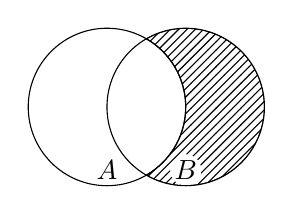
\begin{tikzpicture}
        \begin{scope}[even odd rule]
            \clip  (1,-0.8) circle (0.2) (1,0) circle (1);
            \filldraw [pattern = {north east lines}] (0.5,{0.5*sqrt(3)}) arc (60:-60:1) arc (-120:120:1);
        \end{scope}
        \draw (0,0) circle (1);
        \draw (1,0) circle (1);
        \draw (0,-0.8) node {$A$};
        \draw (1,-0.8) node {$B$};
    \end{tikzpicture}
\end{center}


关联目标:

暂未关联目标



标签: 第一单元

答案: $\{0, 2, 4\}$

解答或提示: 暂无解答与提示

使用记录:

20220510	2022届高三1班	\fcolorbox[rgb]{0,0,0}{1.000,0.000,0}{1.000}


出处: 赋能练习
\item { (000797)}不等式$\dfrac x{x-1}<0$的解集为\blank{50}.


关联目标:

暂未关联目标



标签: 第一单元

答案: $(0,1)$

解答或提示: 暂无解答与提示

使用记录:

20220513	2022届高三1班	\fcolorbox[rgb]{0,0,0}{1.000,0.000,0}{1.000}


出处: 赋能练习
\item { (000816)}不等式$|x-3|<2$的解集为\blank{50}.


关联目标:

暂未关联目标



标签: 第一单元

答案: $\{x|1<x<5\}$

解答或提示: 暂无解答与提示

使用记录:

20220519	2022届高三1班	\fcolorbox[rgb]{0,0,0}{1.000,0.094,0}{0.953}

20220622	2022届高三1班  	\fcolorbox[rgb]{0,0,0}{1.000,0.604,0}{0.698}


出处: 赋能练习
\item { (000836)}已知集合$A=\{1,2,m\}$,$B=\{2,4\}$, 若$A\cup B=\{1,2,3,4\}$, 则实数$m=$\blank{50}.


关联目标:

暂未关联目标



标签: 第一单元

答案: $3$

解答或提示: 暂无解答与提示

使用记录:

20220525	2022届高三1班	\fcolorbox[rgb]{0,0,0}{1.000,0.000,0}{1.000}


出处: 赋能练习
\item { (000846)}已知全集$U=\mathbf{R}$,若集合$A=\{x|\dfrac x{x-1}>0\}$, 则$\complement_U A=$\blank{50}.


关联目标:

暂未关联目标



标签: 第一单元

答案: $[0,1]$

解答或提示: 暂无解答与提示

使用记录:

20220526	2022届高三1班	\fcolorbox[rgb]{0,0,0}{1.000,0.046,0}{0.977}


出处: 赋能练习
\item { (000857)}设集合$A=\{x||x|<2,\ x\in \mathbf{R}\}$, $B=\{x|x^2-4x+3\ge 0, \ x\in \mathbf{R}\}$, 则$A\cap B=$\blank{50}.


关联目标:

暂未关联目标



标签: 第一单元

答案: $(-2,1]$

解答或提示: 暂无解答与提示

使用记录:

20220527	2022届高三1班	\fcolorbox[rgb]{0,0,0}{1.000,0.094,0}{0.953}


出处: 赋能练习
\item { (000879)}若集合$A=\{x|3x+1>0\}$, $B=\{x||x-1|<2\}$, 则$A\cap B$=\blank{50}.


关联目标:

暂未关联目标



标签: 第一单元

答案: $(-\frac 13,3)$

解答或提示: 暂无解答与提示

使用记录:

20220602	2022届高三1班	\fcolorbox[rgb]{0,0,0}{1.000,0.094,0}{0.953}


出处: 赋能练习
\item { (000891)}已知集合$A=\{x||x-2|<a\}$, $B=\{x|x^2-2x-3<0\}$, 若$B\subseteq A$, 则实数$a$的取值范围是\blank{50}.


关联目标:

暂未关联目标



标签: 第一单元

答案: $a\ge 3$

解答或提示: 暂无解答与提示

使用记录:

20220607	2022届高三1班	\fcolorbox[rgb]{0,0,0}{1.000,0.372,0}{0.814}


出处: 赋能练习
\item { (000899)}设集合$M=\{x|x^2=x\}$, $N=\{x|\log_2 x\le 0\}$, 则$M\cup N=$\blank{50}.


关联目标:

暂未关联目标



标签: 第一单元

答案: $[0,1]$

解答或提示: 暂无解答与提示

使用记录:

20220613	2022届高三1班	\fcolorbox[rgb]{0,0,0}{1.000,0.418,0}{0.791}


出处: 赋能练习
\item { (000910)}若集合$A=\{x|y=\sqrt{x-1},\ x\in \mathbf{R}\}$, $B=\{x||x|\le 1,\ x\in \mathbf{R}\}$, 则$A\cap B=$\blank{50}.


关联目标:

暂未关联目标



标签: 第一单元

答案: $\{1\}$

解答或提示: 暂无解答与提示

使用记录:

20220615	2022届高三1班	\fcolorbox[rgb]{0,0,0}{1.000,0.046,0}{0.977}


出处: 赋能练习
\item { (000920)}已知全集$U=\mathbf{R}$, $A=\{x|x^2-2x<0\}$, $B=\{x|x\ge 1\}$, 则$A\cap \complement_U B=$\blank{50}.


关联目标:

暂未关联目标



标签: 第一单元

答案: $(0,1)$

解答或提示: 暂无解答与提示

使用记录:

20220621	2022届高三1班	\fcolorbox[rgb]{0,0,0}{1.000,0.000,0}{1.000}


出处: 赋能练习
\item { (000924)}已知$x,y\in \mathbf{R}^+$, 且满足$\dfrac x3+\dfrac y4=1$, 则$xy$的最大值为\blank{50}.


关联目标:

暂未关联目标



标签: 第一单元

答案: $3$

解答或提示: 暂无解答与提示

使用记录:

20220621	2022届高三1班	\fcolorbox[rgb]{0,0,0}{1.000,0.000,0}{1.000}


出处: 赋能练习
\item { (000932)}集合$A=\{x|x^2-3x<0\}$, $B=\{x||x|<2\}$, 则$A\cup B$等于\blank{50}.


关联目标:

暂未关联目标



标签: 第一单元

答案: $(-2,3)$

解答或提示: 暂无解答与提示

使用记录:

20220622	2022届高三1班	\fcolorbox[rgb]{0,0,0}{1.000,0.094,0}{0.953}


出处: 赋能练习
\item { (000939)}若$m>0$, $n>0$, $m+n=1$, 且$\dfrac t m+\dfrac 1 n$($t>0$)的最小值为$9$, 则$t=$\blank{50}.


关联目标:

暂未关联目标



标签: 第一单元

答案: $4$

解答或提示: 暂无解答与提示

使用记录:

20220622	2022届高三1班	\fcolorbox[rgb]{0,0,0}{1.000,0.186,0}{0.907}


出处: 赋能练习
\item { (000942)}已知集合$A=\{-1,3,2m-1\}$, 集合$B=\{3,m^2\}$. 若$B\subseteq A$, 则实数$m=$\blank{50}.


关联目标:

暂未关联目标



标签: 第一单元

答案: $1$

解答或提示: 暂无解答与提示

使用记录:

20220624	2022届高三1班	\fcolorbox[rgb]{0,0,0}{1.000,0.000,0}{1.000}


出处: 赋能练习
\item { (000964)}已知全集$U=\mathbf{R}$, 集合$A=\{x|(x-1)(x-4)\le 0\}$, 则集合$A$的补集$\complement_UA=$\blank{50}.


关联目标:

暂未关联目标



标签: 第一单元

答案: $(-\infty ,1)\cup (4,+\infty)$

解答或提示: 暂无解答与提示

使用记录:

20220629    2022届高三1班  	\fcolorbox[rgb]{0,0,0}{1.000,0.046,0}{0.977}


出处: 赋能练习
\item { (000975)}下列各句是否是命题? (T or F)\\ 
\blank{30} (1) $1$是偶数;\\ 
\blank{30} (2) 线段$AB$太长;\\ 
\blank{30} (3) 所有有理数都大于零;\\ 
\blank{30} (4) $2>5$;\\ 
\blank{30} (5) 存在实数$a$使$|a|=-a$不成立.


关联目标:

暂未关联目标



标签: 第一单元

答案: 暂无答案

解答或提示: 暂无解答与提示

使用记录:

2016届11班	\fcolorbox[rgb]{0,0,0}{1.000,0.000,0}{1.000}	\fcolorbox[rgb]{0,0,0}{1.000,0.000,0}{1.000}	\fcolorbox[rgb]{0,0,0}{1.000,0.000,0}{1.000}	\fcolorbox[rgb]{0,0,0}{1.000,0.000,0}{1.000}	\fcolorbox[rgb]{0,0,0}{1.000,0.000,0}{1.000}

2016届12班	\fcolorbox[rgb]{0,0,0}{1.000,0.154,0}{0.923}	\fcolorbox[rgb]{0,0,0}{1.000,0.000,0}{1.000}	\fcolorbox[rgb]{0,0,0}{1.000,0.154,0}{0.923}	\fcolorbox[rgb]{0,0,0}{1.000,0.256,0}{0.872}	\fcolorbox[rgb]{0,0,0}{1.000,0.000,0}{1.000}


出处: 2016届创新班作业	1101-命题及其运算
\item { (000976)}在下列各命题的右边写出其否定形式(否定命题).\\ 
(1) $2 \times 2 =5$; \blank{150}.\\ 
(2) $\sqrt{3-\pi}$有意义; \blank{150}.\\ 
(3) $a$不是非负数; \blank{150}.\\ 
(4) $\sqrt{a}$不是无理数; \blank{150}.(本小题中已知$a\ge 0$)\\ 
(5) $x=1$不是方程$x(x+1)=0$的根; \blank{150}.


关联目标:

暂未关联目标



标签: 第一单元

答案: 暂无答案

解答或提示: 暂无解答与提示

使用记录:

2016届11班	\fcolorbox[rgb]{0,0,0}{1.000,0.000,0}{1.000}	\fcolorbox[rgb]{0,0,0}{1.000,0.052,0}{0.974}	\fcolorbox[rgb]{0,0,0}{1.000,0.462,0}{0.769}	\fcolorbox[rgb]{0,0,0}{1.000,0.462,0}{0.769}	\fcolorbox[rgb]{0,0,0}{1.000,0.206,0}{0.897}

2016届12班	\fcolorbox[rgb]{0,0,0}{1.000,0.102,0}{0.949}	\fcolorbox[rgb]{0,0,0}{1.000,0.052,0}{0.974}	\fcolorbox[rgb]{0,0,0}{1.000,0.358,0}{0.821}	\fcolorbox[rgb]{0,0,0}{1.000,0.358,0}{0.821}	\fcolorbox[rgb]{0,0,0}{1.000,0.256,0}{0.872}


出处: 2016届创新班作业	1101-命题及其运算
\item { (000979)}下列各组命题是否互为否定形式(否定命题)? (T or F).\\ 
\blank{30}(1) $a,b$都是偶数; / $a,b$都不是偶数.\\ 
\blank{30}(2) $a,b$不都是偶数; / $a,b$都是偶数.\\ 
\blank{30}(3) $a,b$中至少有一个是偶数; / $a,b$中至多有两个是偶数.\\ 
\blank{30}(4) $a,b$都不是偶数; / $a,b$都是奇数.


关联目标:

暂未关联目标



标签: 第一单元

答案: 暂无答案

解答或提示: 暂无解答与提示

使用记录:

2016届11班	\fcolorbox[rgb]{0,0,0}{1.000,0.102,0}{0.949}	\fcolorbox[rgb]{0,0,0}{1.000,0.154,0}{0.923}	\fcolorbox[rgb]{0,0,0}{1.000,0.000,0}{1.000}	\fcolorbox[rgb]{0,0,0}{1.000,0.000,0}{1.000}

2016届12班	\fcolorbox[rgb]{0,0,0}{1.000,0.052,0}{0.974}	\fcolorbox[rgb]{0,0,0}{1.000,0.102,0}{0.949}	\fcolorbox[rgb]{0,0,0}{1.000,0.052,0}{0.974}	\fcolorbox[rgb]{0,0,0}{1.000,0.000,0}{1.000}


出处: 2016届创新班作业	1101-命题及其运算
\item { (000980)}填写下列各词的否定词. 例如``$\cdots$是$\cdots$''的否定词是``$\cdots$不是$\cdots$''\\ 
(1) ``$\cdots$都不是$\cdots$''; \blank{150}.\\ 
(2) ``$\cdots$中至少有一个是$\cdots$''; \blank{150}.\\ 
(3) ``$\cdots$中至多有$n$个是$\cdots$''; \blank{150}.


关联目标:

暂未关联目标



标签: 第一单元

答案: 暂无答案

解答或提示: 暂无解答与提示

使用记录:

2016届11班	\fcolorbox[rgb]{0,0,0}{1.000,0.564,0}{0.718}	\fcolorbox[rgb]{0,0,0}{1.000,0.154,0}{0.923}	\fcolorbox[rgb]{0,0,0}{1.000,0.154,0}{0.923}

2016届12班	\fcolorbox[rgb]{0,0,0}{1.000,0.308,0}{0.846}	\fcolorbox[rgb]{0,0,0}{1.000,0.102,0}{0.949}	\fcolorbox[rgb]{0,0,0}{1.000,0.358,0}{0.821}


出处: 2016届创新班作业	1101-命题及其运算
\item { (000982)}模仿讲义中的真值表, 列出下列每组逻辑运算的真值表并回答各问题:\\ 
(1) ``非$(\ P$且$Q\ )$''与``$($非$P\ )$或$($非$Q\ )$'' (De Morgan律之一);
\begin{center}
\begin{tabular}{|c|c||c|c||c|c|c||}
\hline
$P$ & $Q$ & $P$且$Q$ & 非$(\ P$且$Q\ )$ & 非$P$ & 非$Q$ & $($非$P\ )$或$($非$Q\ )$\\
\hline
T & T &&&&&\\
\hline
T & F &&&&&\\
\hline
F & T &&&&&\\
\hline
F & F &&&&&\\
\hline\\ 
\end{tabular}
\end{center} 
(2) ``$P$且$(\ Q$且$R\ )$''与``$(\ P$且$Q\ )$且$R$''(模仿(1)完成); 你的结论是什么? 如果把两个运算中的``且''都换成``或'', 结论(毋需证明)又是什么?\\ 
(3) ``$P$且 $(\ Q$或$R\ )$''与``$(\ P$且$Q\ )$或$(\ P$且$R\ )$''(模仿(1)完成); 你的结论是什么? 如果把两个运算中的``且''都换成``或'', 同时把``或''都换成``且'', 结论(毋须证明)又是什么?


关联目标:

暂未关联目标



标签: 第一单元

答案: 暂无答案

解答或提示: 暂无解答与提示

使用记录:

2016届11班	\fcolorbox[rgb]{0,0,0}{1.000,0.358,0}{0.821}	\fcolorbox[rgb]{0,0,0}{1.000,0.564,0}{0.718}	\fcolorbox[rgb]{0,0,0}{1.000,0.770,0}{0.615}

2016届12班	\fcolorbox[rgb]{0,0,0}{1.000,0.206,0}{0.897}	\fcolorbox[rgb]{0,0,0}{0.974,1.000,0}{0.487}	\fcolorbox[rgb]{0,0,0}{0.872,1.000,0}{0.436}


出处: 2016届创新班作业	1101-命题及其运算
\item { (000983)}用反证法证明如下命题:\\ 
(1) 已知$n$是整数. 如果$3$整除$n^3$, 则$3$整除$n$(提示: 讨论$n=3k,3k+1,3k+2$, 其中$k$是整数);\\ 
(2) 如果实数$x$满足$x^{101}-4x^2+8x-1=0$, 则$x>0$;\\ 
(3) $\sqrt[3]{3}$是无理数(提示: 可借鉴讲义上$\sqrt{6}$是无理数的证明方法);\\ 
(4*) $\sqrt{2}+\sqrt{3}$是无理数.


关联目标:

暂未关联目标



标签: 第一单元

答案: 暂无答案

解答或提示: 暂无解答与提示

使用记录:

2016届11班	\fcolorbox[rgb]{0,0,0}{1.000,0.924,0}{0.538}	\fcolorbox[rgb]{0,0,0}{1.000,0.358,0}{0.821}	\fcolorbox[rgb]{0,0,0}{1.000,0.666,0}{0.667}	\fcolorbox[rgb]{0,0,0}{1.000,0.410,0}{0.795}

2016届12班	\fcolorbox[rgb]{0,0,0}{1.000,0.666,0}{0.667}	\fcolorbox[rgb]{0,0,0}{1.000,0.154,0}{0.923}	\fcolorbox[rgb]{0,0,0}{1.000,0.924,0}{0.538}	\fcolorbox[rgb]{0,0,0}{1.000,0.358,0}{0.821}


出处: 2016届创新班作业	1102-反证法
\item { (000984)}已知$a,b$均为实数, 求证:``关于$x$的不等式$ax+b>0$对一切实数均成立''等价于``$a=0$且$b>0$''. (绝对不允许跳步骤)


关联目标:

暂未关联目标



标签: 第一单元

答案: 暂无答案

解答或提示: 暂无解答与提示

使用记录:

2016届11班	\fcolorbox[rgb]{0,0,0}{0.564,1.000,0}{0.282}

2016届12班	\fcolorbox[rgb]{0,0,0}{0.410,1.000,0}{0.205}


出处: 2016届创新班作业	1102-反证法
\item { (000985)}写出下列各命题的逆命题, 否命题, 逆否命题, 并判断真假.\\ 
(1) (已知$a,b$均为实数) 若$a^2+b^2=0$, 则$a=0$. 原命题的真值: \blank{30};\\ 
逆命题: \blank{250}; 逆命题的真值: \blank{30};\\ 
否命题: \blank{250}; 否命题的真值: \blank{30};\\ 
逆否命题: \blank{250}; 逆否命题的真值: \blank{30}.\\ 
(2) 若$ab=0$, 则$a=0$或$b=0$. 原命题的真值: \blank{30};\\ 
逆命题: \blank{250}; 逆命题的真值: \blank{30};\\ 
否命题: \blank{250}; 否命题的真值: \blank{30};\\ 
逆否命题: \blank{250}; 逆否命题的真值: \blank{30}.\\ 
(3) (已知$a,b$均为整数) 若$a,b$都是偶数, 则$a+b$是偶数. 原命题的真值: \blank{30};\\ 
逆命题: \blank{250}; 逆命题的真值: \blank{30};\\ 
否命题: \blank{250}; 否命题的真值: \blank{30};\\ 
逆否命题: \blank{250}; 逆否命题的真值: \blank{30}.\\ 
(4) (已知$a,b$均为整数) 若$ab$是奇数, 则$a,b$中至少有一个是奇数. 原命题的真值: \blank{30};\\ 
逆命题: \blank{250}; 逆命题的真值: \blank{30};\\ 
否命题: \blank{250}; 否命题的真值: \blank{30};\\ 
逆否命题: \blank{250}; 逆否命题的真值: \blank{30}.


关联目标:

暂未关联目标



标签: 第一单元

答案: 暂无答案

解答或提示: 暂无解答与提示

使用记录:

2016届11班	\fcolorbox[rgb]{0,0,0}{1.000,0.052,0}{0.974}	\fcolorbox[rgb]{0,0,0}{1.000,0.256,0}{0.872}	\fcolorbox[rgb]{0,0,0}{1.000,0.308,0}{0.846}	\fcolorbox[rgb]{0,0,0}{1.000,0.256,0}{0.872}

2016届12班	\fcolorbox[rgb]{0,0,0}{1.000,0.052,0}{0.974}	\fcolorbox[rgb]{0,0,0}{1.000,0.154,0}{0.923}	\fcolorbox[rgb]{0,0,0}{1.000,0.308,0}{0.846}	\fcolorbox[rgb]{0,0,0}{1.000,0.462,0}{0.769}


出处: 2016届创新班作业	1103-假言命题的四种形式及充分必要条件
\item { (000987)}已知实数$t\ne 0$. 证明: ``$x=t$是方程$a x^3+b x^2+cx+d=0$的根''的充分必要条件是``$x=\dfrac{1}{t}$是方程$d x^3+c x^2+ b x+a=0$的根''.


关联目标:

暂未关联目标



标签: 第一单元

答案: 暂无答案

解答或提示: 暂无解答与提示

使用记录:

2016届11班	\fcolorbox[rgb]{0,0,0}{1.000,0.462,0}{0.769}

2016届12班	\fcolorbox[rgb]{0,0,0}{1.000,0.512,0}{0.744}


出处: 2016届创新班作业	1103-假言命题的四种形式及充分必要条件
\item { (000988)}已知$a,b,c$均为实数. 证明: 这三个数中``任意两数之和大于第三个数''的充分必要条件是``任意两数之差小于第三个数''.


关联目标:

暂未关联目标



标签: 第一单元

答案: 暂无答案

解答或提示: 暂无解答与提示

使用记录:

2016届11班	\fcolorbox[rgb]{0,0,0}{0.616,1.000,0}{0.308}

2016届12班	\fcolorbox[rgb]{0,0,0}{0.666,1.000,0}{0.333}


出处: 2016届创新班作业	1103-假言命题的四种形式及充分必要条件
\item { (000989)}判断下列各组对象是否组成集合. (T or F)\\ 
\blank{30} (1) 大于$0$的偶数全体.\\ 
\blank{30} (2) 绝对值小于$0$的实数全体.\\ 
\blank{30} (3) 很小的数的全体.


关联目标:

暂未关联目标



标签: 第一单元

答案: 暂无答案

解答或提示: 暂无解答与提示

使用记录:

2016届11班	\fcolorbox[rgb]{0,0,0}{1.000,0.000,0}{1.000}	\fcolorbox[rgb]{0,0,0}{1.000,0.256,0}{0.872}	\fcolorbox[rgb]{0,0,0}{1.000,0.000,0}{1.000}

2016届12班	\fcolorbox[rgb]{0,0,0}{1.000,0.000,0}{1.000}	\fcolorbox[rgb]{0,0,0}{1.000,0.000,0}{1.000}	\fcolorbox[rgb]{0,0,0}{1.000,0.000,0}{1.000}


出处: 2016届创新班作业	1104-集合及其表示
\item { (000990)}用描述法或列举法(自行择其一种)表示下列集合.\\ 
(1) 大于$0$且小于$3$的实数的全体.\\ 
(2) 方程$x^3-x=0$的解的全体.\\ 
(3) 一次函数$y=2x+1$图像上所有点的全体.\\ 
(4) 被$3$除余$2$的整数的全体.


关联目标:

暂未关联目标



标签: 第一单元

答案: 暂无答案

解答或提示: 暂无解答与提示

使用记录:

2016届11班	\fcolorbox[rgb]{0,0,0}{1.000,0.102,0}{0.949}	\fcolorbox[rgb]{0,0,0}{1.000,0.102,0}{0.949}	\fcolorbox[rgb]{0,0,0}{1.000,0.000,0}{1.000}	\fcolorbox[rgb]{0,0,0}{1.000,0.462,0}{0.769}

2016届12班	\fcolorbox[rgb]{0,0,0}{1.000,0.052,0}{0.974}	\fcolorbox[rgb]{0,0,0}{1.000,0.154,0}{0.923}	\fcolorbox[rgb]{0,0,0}{1.000,0.052,0}{0.974}	\fcolorbox[rgb]{0,0,0}{1.000,0.564,0}{0.718}


出处: 2016届创新班作业	1104-集合及其表示
\item { (000991)}用列举法表示下列集合:\\ 
(1) $\left\{x\left| \dfrac{6}{3-x}\in\mathbf{Z},x\in\mathbf{Z}\right.\right\}$;\\ 
(2) $\{(x,y)|x+y=4,x,y\in\mathbf{N}\}$.


关联目标:

暂未关联目标



标签: 第一单元

答案: 暂无答案

解答或提示: 暂无解答与提示

使用记录:

2016届11班	\fcolorbox[rgb]{0,0,0}{1.000,0.512,0}{0.744}	\fcolorbox[rgb]{0,0,0}{1.000,0.000,0}{1.000}

2016届12班	\fcolorbox[rgb]{0,0,0}{1.000,0.564,0}{0.718}	\fcolorbox[rgb]{0,0,0}{1.000,0.102,0}{0.949}


出处: 2016届创新班作业	1104-集合及其表示
\item { (000992)}在直角坐标系中, 用图形表示下列集合:\\ 
(1) $\{(x,y)|\ 2<x<6,1<y<4,x,y\in\mathbf{R}\}$; \hfill (2) $\{(x,y)|\ 2<x<6,1<y<4,x,y\in\mathbf{Z}\}$.


关联目标:

暂未关联目标



标签: 第一单元

答案: 暂无答案

解答或提示: 暂无解答与提示

使用记录:

2016届11班	\fcolorbox[rgb]{0,0,0}{0.770,1.000,0}{0.385}	\fcolorbox[rgb]{0,0,0}{1.000,0.564,0}{0.718}

2016届12班	\fcolorbox[rgb]{0,0,0}{0.512,1.000,0}{0.256}	\fcolorbox[rgb]{0,0,0}{1.000,0.358,0}{0.821}


出处: 2016届创新班作业	1104-集合及其表示
\item { (000993)}集合$\left\{a,\dfrac{b}{a},1\right\}$和$\{0,a+b,a^2\}$ 表示同一个集合, 求实数$a,b$的值.


关联目标:

暂未关联目标



标签: 第一单元

答案: 暂无答案

解答或提示: 暂无解答与提示

使用记录:

2016届11班	\fcolorbox[rgb]{0,0,0}{1.000,0.358,0}{0.821}

2016届12班	\fcolorbox[rgb]{0,0,0}{1.000,0.564,0}{0.718}


出处: 2016届创新班作业	1104-集合及其表示
\item { (000994)}已知$a$是实数, 集合$M=\{x|\ ax^2+2x+a=0\}$有且仅有一个元素. 求满足上述条件的$a$所构成的集合.


关联目标:

暂未关联目标



标签: 第一单元

答案: 暂无答案

解答或提示: 暂无解答与提示

使用记录:

2016届11班	\fcolorbox[rgb]{0,0,0}{1.000,0.616,0}{0.692}

2016届12班	\fcolorbox[rgb]{0,0,0}{1.000,0.616,0}{0.692}


出处: 2016届创新班作业	1104-集合及其表示
\item { (000995)}已知非空集合$M$中的元素都是正整数, 且满足性质: 若$x\in M$, 则$4-x\in M$. 求满足条件的集合$M$.


关联目标:

暂未关联目标



标签: 第一单元

答案: 暂无答案

解答或提示: 暂无解答与提示

使用记录:

2016届11班	\fcolorbox[rgb]{0,0,0}{0.000,1.000,0}{0.000}

2016届12班	\fcolorbox[rgb]{0,0,0}{0.000,1.000,0}{0.000}


出处: 2016届创新班作业	1104-集合及其表示
\item { (000996)}以下各命题中, 真命题有: \blank{80}(可能多选).
\fourch{$\varnothing \in \varnothing$}{$\varnothing \in \{\varnothing\}$}{$\varnothing \subseteq \varnothing$}{$\varnothing \subseteq \{\varnothing\}$}


关联目标:

暂未关联目标



标签: 第一单元

答案: 暂无答案

解答或提示: 暂无解答与提示

使用记录:

2016届11班	\fcolorbox[rgb]{0,0,0}{1.000,0.102,0}{0.949}

2016届12班	\fcolorbox[rgb]{0,0,0}{1.000,0.474,0}{0.763}


出处: 2016届创新班作业	1105-集合的关系
\item { (000997)}以下各命题中, 真命题有: \blank{80}(可能多选).
\fourch{$5\in \{x|x\le 10\}$}{$\{5\} \in \{x|x\le 10\}$}{$\varnothing \in \{1,2,3,4\}$}{$\varnothing \subseteq \{1,2,3,4\}$}


关联目标:

暂未关联目标



标签: 第一单元

答案: 暂无答案

解答或提示: 暂无解答与提示

使用记录:

2016届11班	\fcolorbox[rgb]{0,0,0}{1.000,0.358,0}{0.821}

2016届12班	\fcolorbox[rgb]{0,0,0}{1.000,0.264,0}{0.868}


出处: 2016届创新班作业	1105-集合的关系
\item { (000998)}满足$\{a_1,a_2\}\subseteq A\subsetneqq\{a_1,a_2,a_3,a_4,a_5,a_6\}$的集合$A$的个数是\blank{100}.


关联目标:

暂未关联目标



标签: 第一单元

答案: 暂无答案

解答或提示: 暂无解答与提示

使用记录:

2016届11班	\fcolorbox[rgb]{0,0,0}{1.000,0.206,0}{0.897}

2016届12班	\fcolorbox[rgb]{0,0,0}{1.000,0.422,0}{0.789}


出处: 2016届创新班作业	1105-集合的关系
\item { (000999)}设$A=\{1,2\}$, $B=\{X|X\subseteq A\}$. 则$B=$\blank{150}.


关联目标:

暂未关联目标



标签: 第一单元

答案: 暂无答案

解答或提示: 暂无解答与提示

使用记录:

2016届11班	\fcolorbox[rgb]{0,0,0}{1.000,0.924,0}{0.538}

2016届12班	\fcolorbox[rgb]{0,0,0}{0.422,1.000,0}{0.211}


出处: 2016届创新班作业	1105-集合的关系
\item { (001000)}设$A=\{n|\ n=3k+1,k \in \mathbf{Z}^+\}$, $B=\{n|\ n=3k-2,k \in \mathbf{Z}^+\}$.\\ 
(1) 集合$A$与集合$B$是相等的还是有真包含关系还是没有任何包含关系?\\ 
(2) 证明你的结论.


关联目标:

暂未关联目标



标签: 第一单元

答案: 暂无答案

解答或提示: 暂无解答与提示

使用记录:

2016届11班	\fcolorbox[rgb]{0,0,0}{1.000,0.000,0}{1.000}	\fcolorbox[rgb]{0,0,0}{1.000,0.358,0}{0.821}

2016届12班	\fcolorbox[rgb]{0,0,0}{1.000,0.052,0}{0.974}	\fcolorbox[rgb]{0,0,0}{1.000,0.474,0}{0.763}


出处: 2016届创新班作业	1105-集合的关系
\item { (001001)}证明或否定: $\{y|y\ge 0\}=\{y|y=x^2, x \in \mathbf{R}\}$.


关联目标:

暂未关联目标



标签: 第一单元

答案: 暂无答案

解答或提示: 暂无解答与提示

使用记录:

2016届11班	\fcolorbox[rgb]{0,0,0}{1.000,0.770,0}{0.615}

2016届12班	\fcolorbox[rgb]{0,0,0}{1.000,0.894,0}{0.553}


出处: 2016届创新班作业	1105-集合的关系
\item { (001002)}设$a$是一个实数, 集合$A=\{x|\ x<2\}$, $B=\{x|\ x\leq a\}$, 且$A \subseteq B$.\\ 
(1) 实数$a$的取值范围为\blank{100};\\ 
(2) 试证明(1)的结论.


关联目标:

暂未关联目标



标签: 第一单元

答案: 暂无答案

解答或提示: 暂无解答与提示

使用记录:

2016届11班	\fcolorbox[rgb]{0,0,0}{1.000,0.052,0}{0.974}	\fcolorbox[rgb]{0,0,0}{0.410,1.000,0}{0.205}

2016届12班	\fcolorbox[rgb]{0,0,0}{1.000,0.000,0}{1.000}	\fcolorbox[rgb]{0,0,0}{0.000,1.000,0}{0.000}


出处: 2016届创新班作业	1105-集合的关系
\item { (001004)}设集合$A=\{1,-1\}$, $B=\{x|\ x^2-2ax+b=0,x\in\mathbf{R}\}$, 若$B\subseteq A$且$B\neq\varnothing$, 求实数$a,b$的值.


关联目标:

暂未关联目标



标签: 第一单元

答案: 暂无答案

解答或提示: 暂无解答与提示

使用记录:

2016届11班	\fcolorbox[rgb]{0,0,0}{1.000,0.256,0}{0.872}

2016届12班	\fcolorbox[rgb]{0,0,0}{1.000,0.368,0}{0.816}


出处: 2016届创新班作业	1105-集合的关系
\item { (001005)}设集合$A=\{x|x^2-x+a=0, x \in \mathbf{R}\}$, 求实数$a$的取值范围, 使得$A \subseteq \mathbf{R}^+$.


关联目标:

暂未关联目标



标签: 第一单元

答案: 暂无答案

解答或提示: 暂无解答与提示

使用记录:

2016届11班	\fcolorbox[rgb]{0,0,0}{0.512,1.000,0}{0.256}

2016届12班	\fcolorbox[rgb]{0,0,0}{0.894,1.000,0}{0.447}


出处: 2016届创新班作业	1105-集合的关系
\item { (001006)}设$A=\{a,b,c,d\}$, $B=\{c,d,e,f,g\}$, 则$A \cap B=$\blank{50}.


关联目标:

暂未关联目标



标签: 第一单元

答案: 暂无答案

解答或提示: 暂无解答与提示

使用记录:

2016届11班	\fcolorbox[rgb]{0,0,0}{1.000,0.102,0}{0.949}

2016届12班	\fcolorbox[rgb]{0,0,0}{1.000,0.000,0}{1.000}


出处: 2016届创新班作业	1106-集合的运算
\item { (001007)}设$A=\{1,2\}$, $A\cup B=\{1,2,3\}$, 则$B$为\blank{100}.


关联目标:

暂未关联目标



标签: 第一单元

答案: 暂无答案

解答或提示: 暂无解答与提示

使用记录:

2016届11班	\fcolorbox[rgb]{0,0,0}{1.000,0.102,0}{0.949}

2016届12班	\fcolorbox[rgb]{0,0,0}{1.000,0.206,0}{0.897}


出处: 2016届创新班作业	1106-集合的运算
\item { (001008)}已知集合$P\cap\{4,6\}=\{4\}$, $P\cap\{8,10\}=\{10\}$, $P\cap\{2,12\}=\{12\}$,
若$P\subseteq\{2,4,6,10,12\}$, 则$P=$\blank{50}.


关联目标:

暂未关联目标



标签: 第一单元

答案: 暂无答案

解答或提示: 暂无解答与提示

使用记录:

2016届11班	\fcolorbox[rgb]{0,0,0}{1.000,0.154,0}{0.923}

2016届12班	\fcolorbox[rgb]{0,0,0}{1.000,0.206,0}{0.897}


出处: 2016届创新班作业	1106-集合的运算
\item { (001009)}设$A=\{(x,y)|3x+2y=5\}$, $B=\{(x,y)|x+y=2\}$, 则$A\cap B=$\blank{50}.


关联目标:

暂未关联目标



标签: 第一单元

答案: 暂无答案

解答或提示: 暂无解答与提示

使用记录:

2016届11班	\fcolorbox[rgb]{0,0,0}{1.000,0.154,0}{0.923}

2016届12班	\fcolorbox[rgb]{0,0,0}{1.000,0.154,0}{0.923}


出处: 2016届创新班作业	1106-集合的运算
\item { (001010)}试用集合$A,B,C$的交, 并, 以及关于全集$U$的补运算表示下列文氏图所示的集合.
\begin{center}
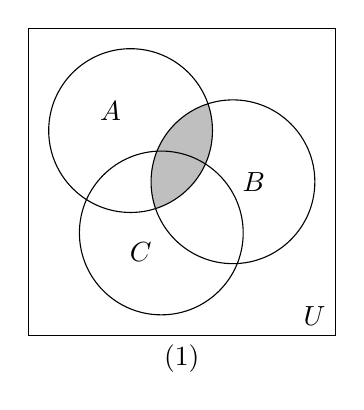
\begin{tikzpicture}[scale = 1.3]
    \begin{scope}
        \clip (1,2) circle (0.8);
        \clip (2,1.5) circle (0.8);     
        \fill [gray!50] (0,0) rectangle (3,3);
    \end{scope}
    \draw (1,2) circle (0.8) node [above left] {$A$};
    \draw (2,1.5) circle (0.8) node [right] {$B$};
    \draw (1.3,1) circle (0.8) node [below left] {$C$};
    \draw (3,0) node [above left] {$U$} rectangle (0,3);
    \draw (1.5,0) node [below] {(1)};   
\end{tikzpicture}
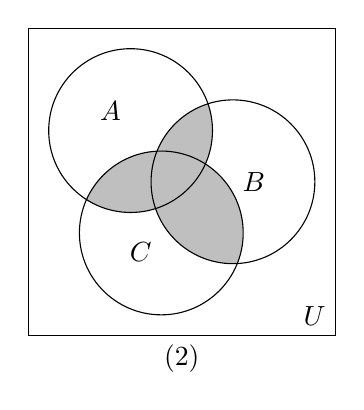
\begin{tikzpicture}[scale = 1.3]
    \begin{scope}
        \clip (1,2) circle (0.8);
        \clip (2,1.5) circle (0.8);     
        \fill [gray!50] (0,0) rectangle (3,3);
    \end{scope}
    \begin{scope}
        \clip (1.3,1) circle (0.8);
        \clip (2,1.5) circle (0.8);     
        \fill [gray!50] (0,0) rectangle (3,3);
    \end{scope}
    \begin{scope}
        \clip (1.3,1) circle (0.8);
        \clip (1,2) circle (0.8);     
        \fill [gray!50] (0,0) rectangle (3,3);
    \end{scope}
    \draw (1,2) circle (0.8) node [above left] {$A$};
    \draw (2,1.5) circle (0.8) node [right] {$B$};
    \draw (1.3,1) circle (0.8) node [below left] {$C$};
    \draw (3,0) node [above left] {$U$} rectangle (0,3);
    \draw (1.5,0) node [below] {(2)};   
\end{tikzpicture}
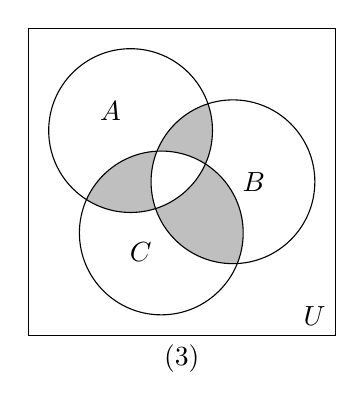
\begin{tikzpicture}[scale = 1.3]
    \begin{scope}[even odd rule]
        \clip (1,2) circle (0.8) (2,1.5) circle (0.8) (1.3,1) circle (0.8) (0,0) rectangle (3,3);
        \fill [gray!50] (1,2) circle (0.8);
        \fill [gray!50] (2,1.5) circle (0.8);
    \end{scope}
    \draw (1,2) circle (0.8) node [above left] {$A$};
    \draw (2,1.5) circle (0.8) node [right] {$B$};
    \draw (1.3,1) circle (0.8) node [below left] {$C$};
    \draw (3,0) node [above left] {$U$} rectangle (0,3);
    \draw (1.5,0) node [below] {(3)};   
\end{tikzpicture}
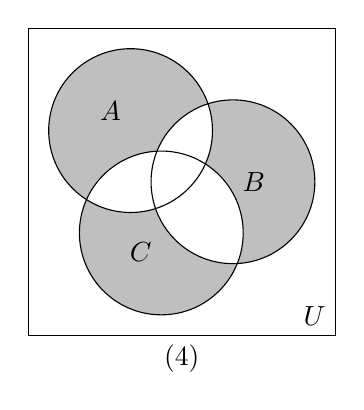
\begin{tikzpicture}[scale = 1.3]
    \begin{scope}[even odd rule]
        \clip (1,2) circle (0.8) (0,0) rectangle (3,3);
        \clip (2,1.5) circle (0.8) (0,0) rectangle (3,3);
        \fill [gray!50] (1.3,1) circle (0.8);
    \end{scope}
    \begin{scope}[even odd rule]
        \clip (1.3,1) circle (0.8) (0,0) rectangle (3,3);
        \clip (2,1.5) circle (0.8) (0,0) rectangle (3,3);
        \fill [gray!50] (1,2) circle (0.8);
    \end{scope}
    \begin{scope}[even odd rule]
        \clip (1,2) circle (0.8) (0,0) rectangle (3,3);
        \clip (1.3,1) circle (0.8) (0,0) rectangle (3,3);
        \fill [gray!50] (2,1.5) circle (0.8);
    \end{scope}
    \draw (1,2) circle (0.8) node [above left] {$A$};
    \draw (2,1.5) circle (0.8) node [right] {$B$};
    \draw (1.3,1) circle (0.8) node [below left] {$C$};
    \draw (3,0) node [above left] {$U$} rectangle (0,3);
    \draw (1.5,0) node [below] {(4)};   
\end{tikzpicture}
\end{center} 
1. \blank{200};2. \blank{200};\\ 
3. \blank{200};4. \blank{200}.


关联目标:

暂未关联目标



标签: 第一单元

答案: 暂无答案

解答或提示: 暂无解答与提示

使用记录:

2016届11班	\fcolorbox[rgb]{0,0,0}{1.000,0.000,0}{1.000}	\fcolorbox[rgb]{0,0,0}{1.000,0.102,0}{0.949}	\fcolorbox[rgb]{0,0,0}{1.000,0.666,0}{0.667}	\fcolorbox[rgb]{0,0,0}{1.000,0.564,0}{0.718}

2016届12班	\fcolorbox[rgb]{0,0,0}{1.000,0.000,0}{1.000}	\fcolorbox[rgb]{0,0,0}{1.000,0.052,0}{0.974}	\fcolorbox[rgb]{0,0,0}{1.000,0.974,0}{0.513}	\fcolorbox[rgb]{0,0,0}{1.000,0.820,0}{0.590}


出处: 2016届创新班作业	1106-集合的运算
\item { (001011)}设全集$U=\{1,2,3,4,5\}$, 若$\complement_U A\cup\complement_U B=\{1,2,4,5\}$, $\complement_U A\cap B=\{5\}$, $ \complement_U B\cap A=\{2\}$, 则$A=$\blank{50}, $B=$\blank{50}.


关联目标:

暂未关联目标



标签: 第一单元

答案: 暂无答案

解答或提示: 暂无解答与提示

使用记录:

2016届11班	\fcolorbox[rgb]{0,0,0}{1.000,0.206,0}{0.897}

2016届12班	\fcolorbox[rgb]{0,0,0}{1.000,0.102,0}{0.949}


出处: 2016届创新班作业	1106-集合的运算
\item { (001012)}$50$名学生做甲, 乙两种实验, 甲做正确者$31$人, 乙做正确者$29$人, 都正确者$21$人, 则两种实验都做错的有\blank{50}人.


关联目标:

暂未关联目标



标签: 第一单元

答案: 暂无答案

解答或提示: 暂无解答与提示

使用记录:

2016届11班	\fcolorbox[rgb]{0,0,0}{1.000,0.154,0}{0.923}

2016届12班	\fcolorbox[rgb]{0,0,0}{1.000,0.102,0}{0.949}


出处: 2016届创新班作业	1106-集合的运算
\item { (001013)}已知集合$M=\{(x,y)|y=x+1, \ x \in \mathbf{R}\}$, $N=\{(x,y)|y=-x^2+4x,\  x \in \mathbf{R}\}$,
则$M \cap N=$\blank{80}.


关联目标:

暂未关联目标



标签: 第一单元

答案: 暂无答案

解答或提示: 暂无解答与提示

使用记录:

2016届11班	\fcolorbox[rgb]{0,0,0}{1.000,0.358,0}{0.821}

2016届12班	\fcolorbox[rgb]{0,0,0}{1.000,0.102,0}{0.949}


出处: 2016届创新班作业	1106-集合的运算
\item { (001017)}设$A,B$是两个集合, 求证: ``$A\cap B=A$''当且仅当``$A \subseteq B$''.(用文氏图画一下并不算证明)


关联目标:

暂未关联目标



标签: 第一单元

答案: 暂无答案

解答或提示: 暂无解答与提示

使用记录:

2016届11班	\fcolorbox[rgb]{0,0,0}{0.512,1.000,0}{0.256}

2016届12班	\fcolorbox[rgb]{0,0,0}{0.358,1.000,0}{0.179}


出处: 2016届创新班作业	1106-集合的运算
\item { (001029)}设$f(x)$是$m$次多项式, $g(x)$是$n$次多项式, $m,n$均为正整数. 判断下列命题的真假(T or F).\\ 
\blank{30} (1) 多项式$-2f(x)$的次数为$m$;\\ 
\blank{30} (2) 多项式$f(x)+g(x)$的次数为$\max\{m,n\}$($\max$表示集合中较大的那个数);\\ 
\blank{30} (3) 多项式$f(x)\times g(x)$的次数为$m+n$;\\ 
\blank{30} (4) 多项式$[f(x)]^2+f(x)+1$的次数为$2m$;


关联目标:

暂未关联目标



标签: 第一单元

答案: 暂无答案

解答或提示: 暂无解答与提示

使用记录:

2016届11班	\fcolorbox[rgb]{0,0,0}{1.000,0.000,0}{1.000}	\fcolorbox[rgb]{0,0,0}{1.000,0.462,0}{0.769}	\fcolorbox[rgb]{0,0,0}{1.000,0.102,0}{0.949}	\fcolorbox[rgb]{0,0,0}{1.000,0.102,0}{0.949}

2016届12班	\fcolorbox[rgb]{0,0,0}{1.000,0.000,0}{1.000}	\fcolorbox[rgb]{0,0,0}{1.000,0.512,0}{0.744}	\fcolorbox[rgb]{0,0,0}{1.000,0.000,0}{1.000}	\fcolorbox[rgb]{0,0,0}{1.000,0.102,0}{0.949}


出处: 2016届创新班作业	1110-多项式的有关概念
\item { (001040)}解方程: $x+\sqrt{2+x}=0$.


关联目标:

暂未关联目标



标签: 第一单元

答案: 暂无答案

解答或提示: 暂无解答与提示

使用记录:

2016届11班	\fcolorbox[rgb]{0,0,0}{1.000,0.102,0}{0.949}

2016届12班	\fcolorbox[rgb]{0,0,0}{1.000,0.256,0}{0.872}


出处: 2016届创新班作业	1112-方程的同解变形
\item { (001041)}解方程: $\dfrac{3}{4x^2+20x+25}=\dfrac{5}{4x^2+8x-5}-\dfrac{2}{4x^2-4x+1}$.


关联目标:

暂未关联目标



标签: 第一单元

答案: 暂无答案

解答或提示: 暂无解答与提示

使用记录:

2016届11班	\fcolorbox[rgb]{0,0,0}{1.000,0.154,0}{0.923}

2016届12班	\fcolorbox[rgb]{0,0,0}{1.000,0.308,0}{0.846}


出处: 2016届创新班作业	1112-方程的同解变形
\item { (001042)}设常数$b\geq 0$, 求证: 方程$\sqrt{f(x)}=b$与方程$f(x)=b^2$同解.


关联目标:

暂未关联目标



标签: 第一单元

答案: 暂无答案

解答或提示: 暂无解答与提示

使用记录:

2016届11班	\fcolorbox[rgb]{0,0,0}{0.512,1.000,0}{0.256}

2016届12班	\fcolorbox[rgb]{0,0,0}{0.820,1.000,0}{0.410}


出处: 2016届创新班作业	1112-方程的同解变形
\item { (001043)}解方程: $\sqrt{1+x}=\sqrt{2x-5}+1$.


关联目标:

暂未关联目标



标签: 第一单元

答案: 暂无答案

解答或提示: 暂无解答与提示

使用记录:

2016届11班	\fcolorbox[rgb]{0,0,0}{1.000,0.718,0}{0.641}

2016届12班	\fcolorbox[rgb]{0,0,0}{1.000,0.770,0}{0.615}


出处: 2016届创新班作业	1112-方程的同解变形
\item { (001044)}(1) 求证: 方程``$\sqrt{f(x)}\sqrt{g(x)}=h(x)$''与
``$f(x)g(x)=(h(x))^2$且$h(x)\geq 0$且$f(x)\geq 0$且$g(x)\geq 0$''同解.\\ 
(2) 试举一例并分析, 说明: 方程``$\sqrt{f(x)}\sqrt{g(x)}=h(x)$''和
``$f(x)g(x)=(h(x))^2$且$h(x)\geq 0$且$f(x)\geq 0$''有时会不同解.


关联目标:

暂未关联目标



标签: 第一单元

答案: 暂无答案

解答或提示: 暂无解答与提示

使用记录:

2016届11班	\fcolorbox[rgb]{0,0,0}{0.770,1.000,0}{0.385}	\fcolorbox[rgb]{0,0,0}{1.000,0.872,0}{0.564}

2016届12班	\fcolorbox[rgb]{0,0,0}{1.000,0.820,0}{0.590}	\fcolorbox[rgb]{0,0,0}{1.000,0.820,0}{0.590}


出处: 2016届创新班作业	1112-方程的同解变形
\item { (001045)}(1) 求证: 方程``$\sqrt{f(x)}+\sqrt{g(x)}=\sqrt{h(x)}$''与方程``$f(x)+g(x)+2\sqrt{f(x)}\sqrt{g(x)}=h(x)$''同解.\\ 
(2) 试举一例并分析, 说明: 方程``$\sqrt{f(x)}+\sqrt{g(x)}=\sqrt{h(x)}$''与方程``$f(x)+g(x)+2\sqrt{f(x)g(x)}=h(x)$''有时会不同解.


关联目标:

暂未关联目标



标签: 第一单元

答案: 暂无答案

解答或提示: 暂无解答与提示

使用记录:

2016届11班	\fcolorbox[rgb]{0,0,0}{1.000,0.718,0}{0.641}	\fcolorbox[rgb]{0,0,0}{1.000,0.872,0}{0.564}

2016届12班	\fcolorbox[rgb]{0,0,0}{1.000,0.308,0}{0.846}	\fcolorbox[rgb]{0,0,0}{1.000,0.924,0}{0.538}


出处: 2016届创新班作业	1112-方程的同解变形
\item { (001046)}解方程: $111x^2+83x-28=0$.


关联目标:

暂未关联目标



标签: 第一单元

答案: 暂无答案

解答或提示: 暂无解答与提示

使用记录:

2016届11班	\fcolorbox[rgb]{0,0,0}{1.000,0.052,0}{0.974}

2016届12班	\fcolorbox[rgb]{0,0,0}{1.000,0.102,0}{0.949}


出处: 2016届创新班作业	1113-一次方程与二次方程
\item { (001047)}解方程: $x^2+x=\sqrt{5}+5$.


关联目标:

暂未关联目标



标签: 第一单元

答案: 暂无答案

解答或提示: 暂无解答与提示

使用记录:

2016届11班	\fcolorbox[rgb]{0,0,0}{1.000,0.052,0}{0.974}

2016届12班	\fcolorbox[rgb]{0,0,0}{1.000,0.052,0}{0.974}


出处: 2016届创新班作业	1113-一次方程与二次方程
\item { (001048)}求实数$a,b$, 使得关于$x$的方程$x^2+2(1+a)x+(3a^2+4ab+4b^2+2)=0$有实根.


关联目标:

暂未关联目标



标签: 第一单元

答案: 暂无答案

解答或提示: 暂无解答与提示

使用记录:

2016届11班	\fcolorbox[rgb]{0,0,0}{1.000,0.206,0}{0.897}

2016届12班	\fcolorbox[rgb]{0,0,0}{1.000,0.154,0}{0.923}


出处: 2016届创新班作业	1113-一次方程与二次方程
\item { (001049)}解关于$x$的方程: $ax-1=x+ab$.


关联目标:

暂未关联目标



标签: 第一单元

答案: 暂无答案

解答或提示: 暂无解答与提示

使用记录:

2016届11班	\fcolorbox[rgb]{0,0,0}{1.000,0.154,0}{0.923}

2016届12班	\fcolorbox[rgb]{0,0,0}{1.000,0.102,0}{0.949}


出处: 2016届创新班作业	1113-一次方程与二次方程
\item { (001050)}解关于$x$的方程: $m^2(x-1)+m(x+3)=6x+2$.


关联目标:

暂未关联目标



标签: 第一单元

答案: 暂无答案

解答或提示: 暂无解答与提示

使用记录:

2016届11班	\fcolorbox[rgb]{0,0,0}{1.000,0.256,0}{0.872}

2016届12班	\fcolorbox[rgb]{0,0,0}{1.000,0.206,0}{0.897}


出处: 2016届创新班作业	1113-一次方程与二次方程
\item { (001051)}已知实数$a,b,c \ne 0$. 解关于$x$的方程: $\dfrac{x-b-c}{a}+\dfrac{x-c-a}{b}+\dfrac{x-a-b}{c}=3$.


关联目标:

暂未关联目标



标签: 第一单元

答案: 暂无答案

解答或提示: 暂无解答与提示

使用记录:

2016届11班	\fcolorbox[rgb]{0,0,0}{1.000,0.666,0}{0.667}

2016届12班	\fcolorbox[rgb]{0,0,0}{1.000,0.666,0}{0.667}


出处: 2016届创新班作业	1113-一次方程与二次方程
\item { (001052)}若关于$x$的方程$2ax=(a+1)x+6$的解集真包含于$\mathbf{Z}^+$, 求$a$.


关联目标:

暂未关联目标



标签: 第一单元

答案: 暂无答案

解答或提示: 暂无解答与提示

使用记录:

2016届11班	\fcolorbox[rgb]{0,0,0}{0.256,1.000,0}{0.128}

2016届12班	\fcolorbox[rgb]{0,0,0}{0.000,1.000,0}{0.000}


出处: 2016届创新班作业	1113-一次方程与二次方程
\item { (001053)}[选做]
解关于$x$的方程: $\dfrac{(x-a)^2}{(x-b)(x-c)}+\dfrac{(x-b)^2}{(x-c)(x-a)}+\dfrac{(x-c)^2}{(x-a)(x-b)}=3$.


关联目标:

暂未关联目标



标签: 第一单元

答案: 暂无答案

解答或提示: 暂无解答与提示

使用记录:

2016届11班	\fcolorbox[rgb]{0,0,0}{0.206,1.000,0}{0.103}

2016届12班	\fcolorbox[rgb]{0,0,0}{0.102,1.000,0}{0.051}


出处: 2016届创新班作业	1113-一次方程与二次方程
\item { (001054)}解方程: $x^4+x^3-7x^2-x+6=0$.


关联目标:

暂未关联目标



标签: 第一单元

答案: 暂无答案

解答或提示: 暂无解答与提示

使用记录:

2016届11班	\fcolorbox[rgb]{0,0,0}{1.000,0.000,0}{1.000}

2016届12班	\fcolorbox[rgb]{0,0,0}{1.000,0.052,0}{0.974}


出处: 2016届创新班作业	1114-高次方程
\item { (001055)}解方程: $2x^5-x^4-15x^3+9x^2+16x+4=0$.


关联目标:

暂未关联目标



标签: 第一单元

答案: 暂无答案

解答或提示: 暂无解答与提示

使用记录:

2016届11班	\fcolorbox[rgb]{0,0,0}{1.000,0.154,0}{0.923}

2016届12班	\fcolorbox[rgb]{0,0,0}{1.000,0.102,0}{0.949}


出处: 2016届创新班作业	1114-高次方程
\item { (001056)}解方程: $(9-16x^2)^3+(16-9x^2)^3+(25x^2-25)^3=0$.


关联目标:

暂未关联目标



标签: 第一单元

答案: 暂无答案

解答或提示: 暂无解答与提示

使用记录:

2016届11班	\fcolorbox[rgb]{0,0,0}{1.000,0.616,0}{0.692}

2016届12班	\fcolorbox[rgb]{0,0,0}{1.000,0.308,0}{0.846}


出处: 2016届创新班作业	1114-高次方程
\item { (001057)}解方程: $2(x^2+6x+1)^2+5(x^2+6x+1)(x^2+1)+2(x^2+1)^2=0$


关联目标:

暂未关联目标



标签: 第一单元

答案: 暂无答案

解答或提示: 暂无解答与提示

使用记录:

2016届11班	\fcolorbox[rgb]{0,0,0}{1.000,0.154,0}{0.923}

2016届12班	\fcolorbox[rgb]{0,0,0}{1.000,0.308,0}{0.846}


出处: 2016届创新班作业	1114-高次方程
\item { (001058)}解方程: $(x+1)(x+3)(x+5)(x+7)=-12$.


关联目标:

暂未关联目标



标签: 第一单元

答案: 暂无答案

解答或提示: 暂无解答与提示

使用记录:

2016届11班	\fcolorbox[rgb]{0,0,0}{1.000,0.102,0}{0.949}

2016届12班	\fcolorbox[rgb]{0,0,0}{1.000,0.256,0}{0.872}


出处: 2016届创新班作业	1114-高次方程
\item { (001059)}解方程: $6x^4+5x^3-38x^2+5x+6=0$.


关联目标:

暂未关联目标



标签: 第一单元

答案: 暂无答案

解答或提示: 暂无解答与提示

使用记录:

2016届11班	\fcolorbox[rgb]{0,0,0}{1.000,0.256,0}{0.872}

2016届12班	\fcolorbox[rgb]{0,0,0}{1.000,0.308,0}{0.846}


出处: 2016届创新班作业	1114-高次方程
\item { (001060)}解方程: $6x^4-25x^3+12x^2+25x+6=0$.


关联目标:

暂未关联目标



标签: 第一单元

答案: 暂无答案

解答或提示: 暂无解答与提示

使用记录:

2016届11班	\fcolorbox[rgb]{0,0,0}{1.000,0.154,0}{0.923}

2016届12班	\fcolorbox[rgb]{0,0,0}{1.000,0.410,0}{0.795}


出处: 2016届创新班作业	1114-高次方程
\item { (001061)}[选做]
解方程: $x^4+8x^3+24x^2+32x+12=0$.


关联目标:

暂未关联目标



标签: 第一单元

答案: 暂无答案

解答或提示: 暂无解答与提示

使用记录:

2016届11班	\fcolorbox[rgb]{0,0,0}{1.000,0.512,0}{0.744}

2016届12班	\fcolorbox[rgb]{0,0,0}{1.000,0.718,0}{0.641}


出处: 2016届创新班作业	1114-高次方程
\item { (001062)}已知关于$x$的方程$x^2+2x-1=0$的两个实根为$x_1,x_2$, 则$x_1+x_2=$\blank{50}, $x_1x_2=$\blank{50}.


关联目标:

暂未关联目标



标签: 第一单元

答案: 暂无答案

解答或提示: 暂无解答与提示

使用记录:

2016届11班	\fcolorbox[rgb]{0,0,0}{1.000,0.000,0}{1.000}

2016届12班	\fcolorbox[rgb]{0,0,0}{1.000,0.000,0}{1.000}


出处: 2016届创新班作业	1115-Viete定理
\item { (001063)}已知关于$x$的方程$ax^2+bx+1=0$有两个实根$\dfrac{1}{2}, \dfrac{1}{3}$, 则$b=$\blank{50}.


关联目标:

暂未关联目标



标签: 第一单元

答案: 暂无答案

解答或提示: 暂无解答与提示

使用记录:

2016届11班	\fcolorbox[rgb]{0,0,0}{1.000,0.102,0}{0.949}

2016届12班	\fcolorbox[rgb]{0,0,0}{1.000,0.052,0}{0.974}


出处: 2016届创新班作业	1115-Viete定理
\item { (001064)}已知关于$x$的方程$x^2+bx-2=0$的一个实根为$2$, 则另一实根为\blank{50}.


关联目标:

暂未关联目标



标签: 第一单元

答案: 暂无答案

解答或提示: 暂无解答与提示

使用记录:

2016届11班	\fcolorbox[rgb]{0,0,0}{1.000,0.000,0}{1.000}

2016届12班	\fcolorbox[rgb]{0,0,0}{1.000,0.000,0}{1.000}


出处: 2016届创新班作业	1115-Viete定理
\item { (001065)}已知关于$x$的方程$-x^2-3x+3=0$的两个实根为$x_1,x_2$, 则$\dfrac{x_1}{x_2}+\dfrac{x_2}{x_1}=$\blank{50}.


关联目标:

暂未关联目标



标签: 第一单元

答案: 暂无答案

解答或提示: 暂无解答与提示

使用记录:

2016届11班	\fcolorbox[rgb]{0,0,0}{1.000,0.102,0}{0.949}

2016届12班	\fcolorbox[rgb]{0,0,0}{1.000,0.102,0}{0.949}


出处: 2016届创新班作业	1115-Viete定理
\item { (001066)}已知关于$x$的二次方程$ax^2+bx+c=0$的两实根为$x_1,x_2$, 则$|x_1-x_2|=$\blank{50}.


关联目标:

暂未关联目标



标签: 第一单元

答案: 暂无答案

解答或提示: 暂无解答与提示

使用记录:

2016届11班	\fcolorbox[rgb]{0,0,0}{1.000,0.308,0}{0.846}

2016届12班	\fcolorbox[rgb]{0,0,0}{1.000,0.512,0}{0.744}


出处: 2016届创新班作业	1115-Viete定理
\item { (001067)}已知关于$x$的方程$x^2+2mx+6=0$的两实根的倒数之和为$1$, 则实数$m=$\blank{50}.


关联目标:

暂未关联目标



标签: 第一单元

答案: 暂无答案

解答或提示: 暂无解答与提示

使用记录:

2016届11班	\fcolorbox[rgb]{0,0,0}{1.000,0.000,0}{1.000}

2016届12班	\fcolorbox[rgb]{0,0,0}{1.000,0.000,0}{1.000}


出处: 2016届创新班作业	1115-Viete定理
\item { (001068)}关于$y$的方程$4y^2+(b^2-3b-10)y+4b=0$的两个实根互为相反数, 则实数$b=$\blank{50}.


关联目标:

暂未关联目标



标签: 第一单元

答案: 暂无答案

解答或提示: 暂无解答与提示

使用记录:

2016届11班	\fcolorbox[rgb]{0,0,0}{1.000,0.206,0}{0.897}

2016届12班	\fcolorbox[rgb]{0,0,0}{1.000,0.102,0}{0.949}


出处: 2016届创新班作业	1115-Viete定理
\item { (001069)}若关于$x$的方程$x^2-mx+2m-2=0$的两实根的平方和为$1$, 则实数$m=$\blank{50}.


关联目标:

暂未关联目标



标签: 第一单元

答案: 暂无答案

解答或提示: 暂无解答与提示

使用记录:

2016届11班	\fcolorbox[rgb]{0,0,0}{1.000,0.102,0}{0.949}

2016届12班	\fcolorbox[rgb]{0,0,0}{1.000,0.410,0}{0.795}


出处: 2016届创新班作业	1115-Viete定理
\item { (001070)}方程组$\left\{
\begin{array}{l}
x+y+xy=5,\\
x^2y+xy^2=6
\end{array}
\right.$的解为$(x,y)=$\blank{200}.


关联目标:

暂未关联目标



标签: 第一单元

答案: 暂无答案

解答或提示: 暂无解答与提示

使用记录:

2016届11班	\fcolorbox[rgb]{0,0,0}{1.000,0.102,0}{0.949}

2016届12班	\fcolorbox[rgb]{0,0,0}{1.000,0.000,0}{1.000}


出处: 2016届创新班作业	1115-Viete定理
\item { (001071)}方程组$\left\{
\begin{array}{l}
x-y=3,\\
xy=-2
\end{array}
\right.$的解为$(x,y)=$\blank{200}.


关联目标:

暂未关联目标



标签: 第一单元

答案: 暂无答案

解答或提示: 暂无解答与提示

使用记录:

2016届11班	\fcolorbox[rgb]{0,0,0}{1.000,0.154,0}{0.923}

2016届12班	\fcolorbox[rgb]{0,0,0}{1.000,0.052,0}{0.974}


出处: 2016届创新班作业	1115-Viete定理
\item { (001072)}关于$x$的方程$x^2+px+q=0$的两个实根之比为$1:2$, 判别式的值为$1$, 求实数$p,q$.


关联目标:

暂未关联目标



标签: 第一单元

答案: 暂无答案

解答或提示: 暂无解答与提示

使用记录:

2016届11班	\fcolorbox[rgb]{0,0,0}{1.000,0.102,0}{0.949}

2016届12班	\fcolorbox[rgb]{0,0,0}{1.000,0.358,0}{0.821}


出处: 2016届创新班作业	1115-Viete定理
\item { (001073)}已知$\alpha,\beta$是关于$x$的二次方程$x^2+(p-2)x+1=0$的两根. 试求$(1+p\alpha+\alpha^2)(1+p\beta+\beta^2)$的值.


关联目标:

暂未关联目标



标签: 第一单元

答案: 暂无答案

解答或提示: 暂无解答与提示

使用记录:

2016届11班	\fcolorbox[rgb]{0,0,0}{1.000,0.256,0}{0.872}

2016届12班	\fcolorbox[rgb]{0,0,0}{1.000,0.206,0}{0.897}


出处: 2016届创新班作业	1115-Viete定理
\item { (001074)}设$\alpha,\beta$是方程$2x^2+x-7=0$的两根, 试以$\dfrac{1}{\alpha^2-1},\dfrac{1}{\beta^2-1}$为根作一个新的二次方程.


关联目标:

暂未关联目标



标签: 第一单元

答案: 暂无答案

解答或提示: 暂无解答与提示

使用记录:

2016届11班	\fcolorbox[rgb]{0,0,0}{1.000,0.462,0}{0.769}

2016届12班	\fcolorbox[rgb]{0,0,0}{1.000,0.512,0}{0.744}


出处: 2016届创新班作业	1115-Viete定理
\item { (001075)}设常数$k\in\mathbf{N}$, 若关于$x$的方程$x^2=2(k+1)x-(k^2+4k-3)$的两个实根符号相反, 求$k$的值,
并解此方程.


关联目标:

暂未关联目标



标签: 第一单元

答案: 暂无答案

解答或提示: 暂无解答与提示

使用记录:

2016届11班	\fcolorbox[rgb]{0,0,0}{1.000,0.206,0}{0.897}

2016届12班	\fcolorbox[rgb]{0,0,0}{1.000,0.102,0}{0.949}


出处: 2016届创新班作业	1115-Viete定理
\item { (001076)}设常数$a>0,m>0$, 若方程组$\left\{
\begin{array}{l}
y^2=4a(x+a),\\
x+y+m=0
\end{array}
\right.$有两组不同的解$(x_1,y_1)$,$(x_2,y_2)$,\\ 
(1) 求$a,m$所满足的条件;\\ 
(2) 用$a,m$表示$\sqrt{(x_1-x_2)^2+(y_1-y_2)^2}$.


关联目标:

暂未关联目标



标签: 第一单元

答案: 暂无答案

解答或提示: 暂无解答与提示

使用记录:

2016届11班	\fcolorbox[rgb]{0,0,0}{1.000,0.564,0}{0.718}	\fcolorbox[rgb]{0,0,0}{1.000,0.820,0}{0.590}

2016届12班	\fcolorbox[rgb]{0,0,0}{1.000,0.308,0}{0.846}	\fcolorbox[rgb]{0,0,0}{1.000,0.616,0}{0.692}


出处: 2016届创新班作业	1115-Viete定理
\item { (001077)}[选做]
解方程组: $\left\{
\begin{array}{l}
x+y+z=15,\\
x^2+y^2+z^2=83,\\
x^3+y^3+z^3=495.
\end{array}\right.$


关联目标:

暂未关联目标



标签: 第一单元

答案: 暂无答案

解答或提示: 暂无解答与提示

使用记录:

2016届11班	\fcolorbox[rgb]{0,0,0}{1.000,0.358,0}{0.821}

2016届12班	\fcolorbox[rgb]{0,0,0}{1.000,0.616,0}{0.692}


出处: 2016届创新班作业	1115-Viete定理
\item { (001078)}解方程: $1+\dfrac{1}{1+\dfrac{1}{1+\dfrac{1}{1+\dfrac{1}{x}}}}=2$.


关联目标:

暂未关联目标



标签: 第一单元

答案: 暂无答案

解答或提示: 暂无解答与提示

使用记录:

2016届11班	\fcolorbox[rgb]{0,0,0}{1.000,0.206,0}{0.897}

2016届12班	\fcolorbox[rgb]{0,0,0}{1.000,0.256,0}{0.872}


出处: 2016届创新班作业	1116-分式方程与无理方程
\item { (001079)}解方程: $\dfrac{x^4-(x-1)^2}{(x^2+1)^2-x^2}+\dfrac{x^2-(x^2-1)^2}{x^2(x+1)^2-1}+\dfrac{x^2(x-1)^2-1}{x^4-(x+1)^2}=x^2$.


关联目标:

暂未关联目标



标签: 第一单元

答案: 暂无答案

解答或提示: 暂无解答与提示

使用记录:

2016届11班	\fcolorbox[rgb]{0,0,0}{1.000,0.616,0}{0.692}

2016届12班	\fcolorbox[rgb]{0,0,0}{1.000,0.462,0}{0.769}


出处: 2016届创新班作业	1116-分式方程与无理方程
\item { (001080)}[选做]
解方程: $\dfrac{1}{(x-5)(x-4)}+\dfrac{1}{(x-4)(x-3)}+\cdots+\dfrac{1}{(x+4)(x+5)}=\dfrac{10}{11}$.


关联目标:

暂未关联目标



标签: 第一单元

答案: 暂无答案

解答或提示: 暂无解答与提示

使用记录:

2016届11班	\fcolorbox[rgb]{0,0,0}{1.000,0.974,0}{0.513}

2016届12班	\fcolorbox[rgb]{0,0,0}{1.000,0.820,0}{0.590}


出处: 2016届创新班作业	1116-分式方程与无理方程
\item { (001081)}解方程: $\sqrt[3]{3-\sqrt{x+1}}+\sqrt[3]{2}=0$.


关联目标:

暂未关联目标



标签: 第一单元

答案: 暂无答案

解答或提示: 暂无解答与提示

使用记录:

2016届11班	\fcolorbox[rgb]{0,0,0}{1.000,0.206,0}{0.897}

2016届12班	\fcolorbox[rgb]{0,0,0}{1.000,0.000,0}{1.000}


出处: 2016届创新班作业	1116-分式方程与无理方程
\item { (001082)}解方程: $\sqrt{3x+4}+2=3\sqrt[4]{3x+4}$.


关联目标:

暂未关联目标



标签: 第一单元

答案: 暂无答案

解答或提示: 暂无解答与提示

使用记录:

2016届11班	\fcolorbox[rgb]{0,0,0}{1.000,0.206,0}{0.897}

2016届12班	\fcolorbox[rgb]{0,0,0}{1.000,0.206,0}{0.897}


出处: 2016届创新班作业	1116-分式方程与无理方程
\item { (001083)}已知$a>b$, $a,b\in \mathbf{R}$. 解关于$y$的方程: $\sqrt{a-y}+\sqrt{y-b}=\sqrt{a-b}$.


关联目标:

暂未关联目标



标签: 第一单元

答案: 暂无答案

解答或提示: 暂无解答与提示

使用记录:

2016届11班	\fcolorbox[rgb]{0,0,0}{1.000,0.052,0}{0.974}

2016届12班	\fcolorbox[rgb]{0,0,0}{1.000,0.102,0}{0.949}


出处: 2016届创新班作业	1116-分式方程与无理方程
\item { (001084)}[选做]
解方程: $\sqrt[4]{97-x}+\sqrt[4]{x}=5$.


关联目标:

暂未关联目标



标签: 第一单元

答案: 暂无答案

解答或提示: 暂无解答与提示

使用记录:

2016届11班	\fcolorbox[rgb]{0,0,0}{1.000,0.820,0}{0.590}

2016届12班	\fcolorbox[rgb]{0,0,0}{0.872,1.000,0}{0.436}


出处: 2016届创新班作业	1116-分式方程与无理方程
\item { (001085)}判断题: (如果正确请在题目前面的横线上写``T'', 错误请在题目前面的横线上写``F'')\\ 
\blank{30}(1) 若$a>b$, $c=d$, 则$ac>bd$;\\ 
\blank{30}(2) 若$\dfrac{a}{c^2}<\dfrac{b}{c^2}$, 则$a<b$;\\ 
\blank{30}(3) 若$ac<bc$, 则$a<b$;\\ 
\blank{30}(4) 若$a>b$, 则$ac^2>bc^2$;\\ 
\blank{30}(5) 若$a>b,c<d$, 则$ac>bd$;\\ 
\blank{30}(6) 若$a>b>0$, $c>d>0$, 则$\dfrac{a}{c}>\dfrac{b}{d}$;\\ 
\blank{30}(7) 若$a>b$, $c\geq d$, 则$a+c>b+d$;\\ 
\blank{30}(8) 若$a>b$, $c\geq d$, 则$a+c\geq b+d$;\\ 
\blank{30}(9) 若$\sqrt[3]{a}>\sqrt[3]{b}$, 则$a>b$.\\ 
\blank{30}(10) 若$ab^2\geq 0$, 则$a\geq 0$.


关联目标:

暂未关联目标



标签: 第一单元

答案: 暂无答案

解答或提示: 暂无解答与提示

使用记录:

2016届11班	\fcolorbox[rgb]{0,0,0}{1.000,0.000,0}{1.000}	\fcolorbox[rgb]{0,0,0}{1.000,0.052,0}{0.974}	\fcolorbox[rgb]{0,0,0}{1.000,0.052,0}{0.974}	\fcolorbox[rgb]{0,0,0}{1.000,0.154,0}{0.923}	\fcolorbox[rgb]{0,0,0}{1.000,0.000,0}{1.000}	\fcolorbox[rgb]{0,0,0}{1.000,0.052,0}{0.974}	\fcolorbox[rgb]{0,0,0}{1.000,0.000,0}{1.000}	\fcolorbox[rgb]{0,0,0}{1.000,0.616,0}{0.692}	\fcolorbox[rgb]{0,0,0}{1.000,0.000,0}{1.000}	\fcolorbox[rgb]{0,0,0}{0.924,1.000,0}{0.462}

2016届12班	\fcolorbox[rgb]{0,0,0}{1.000,0.052,0}{0.974}	\fcolorbox[rgb]{0,0,0}{1.000,0.154,0}{0.923}	\fcolorbox[rgb]{0,0,0}{1.000,0.052,0}{0.974}	\fcolorbox[rgb]{0,0,0}{1.000,0.308,0}{0.846}	\fcolorbox[rgb]{0,0,0}{1.000,0.000,0}{1.000}	\fcolorbox[rgb]{0,0,0}{1.000,0.000,0}{1.000}	\fcolorbox[rgb]{0,0,0}{1.000,0.000,0}{1.000}	\fcolorbox[rgb]{0,0,0}{1.000,0.872,0}{0.564}	\fcolorbox[rgb]{0,0,0}{1.000,0.000,0}{1.000}	\fcolorbox[rgb]{0,0,0}{1.000,0.820,0}{0.590}


出处: 2016届创新班作业	1117-不等式的性质
\item { (001086)}设$\{a,b,m,n\}\subseteq\mathbf{R}^+$且$a>b$, 将$\dfrac{a}{b},\dfrac{b}{a},\dfrac{a+m}{b+m},\dfrac{b+n}{a+n}$按由大到小的次序排列:\\
\blank{40}$>$\blank{40}$>$\blank{40}$>$\blank{40}.


关联目标:

暂未关联目标



标签: 第一单元

答案: 暂无答案

解答或提示: 暂无解答与提示

使用记录:

2016届11班	\fcolorbox[rgb]{0,0,0}{1.000,0.358,0}{0.821}

2016届12班	\fcolorbox[rgb]{0,0,0}{1.000,0.308,0}{0.846}


出处: 2016届创新班作业	1117-不等式的性质
\item { (001087)}证明: 若$a>b$, $c\in\mathbf{R}$, $d<0$, 则$(a-c)d<(b-c)d$.


关联目标:

暂未关联目标



标签: 第一单元

答案: 暂无答案

解答或提示: 暂无解答与提示

使用记录:

2016届11班	\fcolorbox[rgb]{0,0,0}{1.000,0.052,0}{0.974}

2016届12班	\fcolorbox[rgb]{0,0,0}{1.000,0.000,0}{1.000}


出处: 2016届创新班作业	1117-不等式的性质
\item { (001088)}证明: 若$a_1>b_1>0,a_2>b_2>0,a_3>b_3>0$, 则$a_1a_2a_3>b_1b_2b_3$.


关联目标:

暂未关联目标



标签: 第一单元

答案: 暂无答案

解答或提示: 暂无解答与提示

使用记录:

2016届11班	\fcolorbox[rgb]{0,0,0}{1.000,0.410,0}{0.795}

2016届12班	\fcolorbox[rgb]{0,0,0}{1.000,0.206,0}{0.897}


出处: 2016届创新班作业	1117-不等式的性质
\item { (001089)}证明: 若$a>b>0$, $c>d>0$, 则$\dfrac{1}{ac}<\dfrac{1}{bd}$.


关联目标:

暂未关联目标



标签: 第一单元

答案: 暂无答案

解答或提示: 暂无解答与提示

使用记录:

2016届11班	\fcolorbox[rgb]{0,0,0}{1.000,0.308,0}{0.846}

2016届12班	\fcolorbox[rgb]{0,0,0}{1.000,0.256,0}{0.872}


出处: 2016届创新班作业	1117-不等式的性质
\item { (001090)}设常数$a,b\in\mathbf{R}$, 比较以下各组两数的大小:\\ 
(1) $-(a+1)^2$与$-2a^2-3a-4$;\\ 
(2) $a^2+ab+b^2$与$0$.


关联目标:

暂未关联目标



标签: 第一单元

答案: 暂无答案

解答或提示: 暂无解答与提示

使用记录:

2016届11班	\fcolorbox[rgb]{0,0,0}{1.000,0.052,0}{0.974}	\fcolorbox[rgb]{0,0,0}{0.820,1.000,0}{0.410}

2016届12班	\fcolorbox[rgb]{0,0,0}{1.000,0.206,0}{0.897}	\fcolorbox[rgb]{0,0,0}{0.308,1.000,0}{0.154}


出处: 2016届创新班作业	1117-不等式的性质
\item { (001091)}证明:\\ 
(1) 若$a>b$, 则$a^3>b^3$;\\ 
(2)(选做) 若$a>b$, 则$a^5>b^5$.


关联目标:

暂未关联目标



标签: 第一单元

答案: 暂无答案

解答或提示: 暂无解答与提示

使用记录:

2016届11班	\fcolorbox[rgb]{0,0,0}{1.000,0.564,0}{0.718}	\fcolorbox[rgb]{0,0,0}{0.512,1.000,0}{0.256}

2016届12班	\fcolorbox[rgb]{0,0,0}{1.000,0.666,0}{0.667}	\fcolorbox[rgb]{0,0,0}{0.770,1.000,0}{0.385}


出处: 2016届创新班作业	1117-不等式的性质
\item { (001092)}设$a,b\in\mathbf{R}$且$-1<a<1,1<b<3$, 求证:\\ 
(1) $-4<a-b<0$;\\ 
(2)(选做) 任取$x\in(-4,0)$, 总存在满足条件的$a,b$, 使得$a-b=x$(两小题的结论放在一起, 也就是所谓的``$a-b$的取值范围为$(-4,0)$'', 前者表示不会超出这个范围, 后者表示该范围内的每个值都能取到).


关联目标:

暂未关联目标



标签: 第一单元

答案: 暂无答案

解答或提示: 暂无解答与提示

使用记录:

2016届11班	\fcolorbox[rgb]{0,0,0}{1.000,0.206,0}{0.897}	\fcolorbox[rgb]{0,0,0}{0.256,1.000,0}{0.128}

2016届12班	\fcolorbox[rgb]{0,0,0}{1.000,0.052,0}{0.974}	\fcolorbox[rgb]{0,0,0}{0.052,1.000,0}{0.026}


出处: 2016届创新班作业	1117-不等式的性质
\item { (001093)}判断题: (如果同解请在题目前面的横线上写``T'', 否则写``F'')\\ 
\blank{30}(1) $x^2+5x>4$, $x^2+5x+3x>4+3x$;\\ 
\blank{30}(2) $x^2-2x<3$, $\dfrac{x^2-2x}{x-1}<\dfrac{3}{x-1}$;\\ 
\blank{30}(3) $(x-3)(x-5)^2>(2x+1)(x-5)^2$, $x-3>2x+1$;\\ 
\blank{30}(4) $x\ge 1$, $x(x-5)^2\ge (x-5)^2$;\\ 
\blank{30}(5) $x>5$, $x+\dfrac{1}{x^2-3x+2}> 5+\dfrac{1}{x^2-3x+2}$;\\ 
\blank{30}(6) $x<5$, $x+\dfrac{1}{x^2-3x+2}< 5+\dfrac{1}{x^2-3x+2}$;\\ 
\blank{30}(7) $x+\dfrac{1}{x-3}>1+\dfrac{1}{x-3}$, $x>1$;\\ 
\blank{30}(8) $\dfrac{(x+3)(x+1)}{x+1}>0$, $x+3>0$;\\ 
\blank{30}(9) $\dfrac{(x-3)(x+1)}{x+1}>0$, $x-3>0$;\\ 
\blank{30}(10) $|x|<3$, $-3<x<3$.


关联目标:

暂未关联目标



标签: 第一单元

答案: 暂无答案

解答或提示: 暂无解答与提示

使用记录:

2016届11班	\fcolorbox[rgb]{0,0,0}{1.000,0.000,0}{1.000}	\fcolorbox[rgb]{0,0,0}{1.000,0.052,0}{0.974}	\fcolorbox[rgb]{0,0,0}{1.000,0.102,0}{0.949}	\fcolorbox[rgb]{0,0,0}{1.000,0.358,0}{0.821}	\fcolorbox[rgb]{0,0,0}{1.000,0.000,0}{1.000}	\fcolorbox[rgb]{0,0,0}{1.000,0.052,0}{0.974}	\fcolorbox[rgb]{0,0,0}{1.000,0.000,0}{1.000}	\fcolorbox[rgb]{0,0,0}{1.000,0.000,0}{1.000}	\fcolorbox[rgb]{0,0,0}{1.000,0.052,0}{0.974}	\fcolorbox[rgb]{0,0,0}{1.000,0.000,0}{1.000}

2016届12班	\fcolorbox[rgb]{0,0,0}{1.000,0.000,0}{1.000}	\fcolorbox[rgb]{0,0,0}{1.000,0.000,0}{1.000}	\fcolorbox[rgb]{0,0,0}{1.000,0.308,0}{0.846}	\fcolorbox[rgb]{0,0,0}{1.000,0.308,0}{0.846}	\fcolorbox[rgb]{0,0,0}{1.000,0.000,0}{1.000}	\fcolorbox[rgb]{0,0,0}{1.000,0.000,0}{1.000}	\fcolorbox[rgb]{0,0,0}{1.000,0.000,0}{1.000}	\fcolorbox[rgb]{0,0,0}{1.000,0.000,0}{1.000}	\fcolorbox[rgb]{0,0,0}{1.000,0.052,0}{0.974}	\fcolorbox[rgb]{0,0,0}{1.000,0.000,0}{1.000}


出处: 2016届创新班作业	1118-不等式的同解变形
\item { (001094)}(1) 证明或否定: ``$|f(x)|>g(x)$''和``$f(x)>g(x)$且$-f(x)>g(x)$''等价;\\ 
(2) 证明或否定: ``$|f(x)|<g(x)$''和``$f(x)<g(x)$且$-f(x)<g(x)$''等价.


关联目标:

暂未关联目标



标签: 第一单元

答案: 暂无答案

解答或提示: 暂无解答与提示

使用记录:

2016届11班	\fcolorbox[rgb]{0,0,0}{1.000,0.102,0}{0.949}	\fcolorbox[rgb]{0,0,0}{1.000,0.770,0}{0.615}

2016届12班	\fcolorbox[rgb]{0,0,0}{1.000,0.462,0}{0.769}	\fcolorbox[rgb]{0,0,0}{1.000,0.974,0}{0.513}


出处: 2016届创新班作业	1118-不等式的同解变形
\item { (001095)}证明或否定: ``$\sqrt{f(x)}>g(x)$''和
``$\left\{\begin{array}{l}f(x)>g^2(x),\\g(x)\ge 0,\end{array}\right.\ \text{或} \ \left\{\begin{array}{l}f(x)\ge 0,\\g(x)<0\end{array}\right.$''
同解.


关联目标:

暂未关联目标



标签: 第一单元

答案: 暂无答案

解答或提示: 暂无解答与提示

使用记录:

2016届11班	\fcolorbox[rgb]{0,0,0}{1.000,0.206,0}{0.897}

2016届12班	\fcolorbox[rgb]{0,0,0}{1.000,0.206,0}{0.897}


出处: 2016届创新班作业	1118-不等式的同解变形
\item { (001096)}利用绝对值的三角不等式$|a+b|\le |a|+|b|$, 证明:\\ 
(1) 对任意$x,y\in\mathbf{R}$, $|x-y|\ge |x|-|y|$;\\ 
(2) 对任意$x,y\in\mathbf{R}$, $|x-y|\ge ||x|-|y||$.


关联目标:

暂未关联目标



标签: 第一单元

答案: 暂无答案

解答或提示: 暂无解答与提示

使用记录:

2016届11班	\fcolorbox[rgb]{0,0,0}{1.000,0.564,0}{0.718}	\fcolorbox[rgb]{0,0,0}{0.770,1.000,0}{0.385}

2016届12班	\fcolorbox[rgb]{0,0,0}{1.000,0.718,0}{0.641}	\fcolorbox[rgb]{0,0,0}{0.872,1.000,0}{0.436}


出处: 2016届创新班作业	1119-含有绝对值的不等式基本性质
\item { (001097)}已知$|x-a|\le \dfrac{\varepsilon}{2}$, $|y-b|<\dfrac{\varepsilon}{2}$. 求证:\\ 
(1) $|(x+y)-(a+b)|<\varepsilon$;\\ 
(2) $|(x-y)-(a-b)|<\varepsilon$.


关联目标:

暂未关联目标



标签: 第一单元

答案: 暂无答案

解答或提示: 暂无解答与提示

使用记录:

2016届11班	\fcolorbox[rgb]{0,0,0}{1.000,0.000,0}{1.000}	\fcolorbox[rgb]{0,0,0}{1.000,0.000,0}{1.000}

2016届12班	\fcolorbox[rgb]{0,0,0}{1.000,0.052,0}{0.974}	\fcolorbox[rgb]{0,0,0}{1.000,0.052,0}{0.974}


出处: 2016届创新班作业	1119-含有绝对值的不等式基本性质
\item { (001098)}已知$|x|<\dfrac{\varepsilon}{3}$, $|y|<\dfrac{\varepsilon}{6}$, $|z|<\dfrac{\varepsilon}{9}$. 求证: $|x-2y+3z|<\varepsilon$.


关联目标:

暂未关联目标



标签: 第一单元

答案: 暂无答案

解答或提示: 暂无解答与提示

使用记录:

2016届11班	\fcolorbox[rgb]{0,0,0}{1.000,0.000,0}{1.000}

2016届12班	\fcolorbox[rgb]{0,0,0}{1.000,0.000,0}{1.000}


出处: 2016届创新班作业	1119-含有绝对值的不等式基本性质
\item { (001099)}已知常数$\varepsilon>0$, 证明存在实常数$N$, 使得当正整数$n>N$时, $\left|\dfrac{n}{2n+3}-\dfrac{1}{2}\right|<\varepsilon$.


关联目标:

暂未关联目标



标签: 第一单元

答案: 暂无答案

解答或提示: 暂无解答与提示

使用记录:

2016届11班	\fcolorbox[rgb]{0,0,0}{1.000,0.872,0}{0.564}

2016届12班	\fcolorbox[rgb]{0,0,0}{0.718,1.000,0}{0.359}


出处: 2016届创新班作业	1119-含有绝对值的不等式基本性质
\item { (001100)}解下列关于$x$的不等式.\\ 
(1) $ax\le b$;\\ 
(2) $ax+b^2>bx+a^2$;\\ 
(3) $m(mx-1)<2(2x-1)$.


关联目标:

暂未关联目标



标签: 第一单元

答案: 暂无答案

解答或提示: 暂无解答与提示

使用记录:

2016届11班	\fcolorbox[rgb]{0,0,0}{1.000,0.206,0}{0.897}	\fcolorbox[rgb]{0,0,0}{1.000,0.358,0}{0.821}	\fcolorbox[rgb]{0,0,0}{1.000,0.564,0}{0.718}

2016届12班	\fcolorbox[rgb]{0,0,0}{1.000,0.270,0}{0.865}	\fcolorbox[rgb]{0,0,0}{1.000,0.108,0}{0.946}	\fcolorbox[rgb]{0,0,0}{1.000,0.540,0}{0.730}


出处: 2016届创新班作业	1120-一次不等式
\item { (001101)}求不等式$3x-1>2-\dfrac{x+1}{3}\ge 1-\dfrac{2x-3}{2}$的解集.


关联目标:

暂未关联目标



标签: 第一单元

答案: 暂无答案

解答或提示: 暂无解答与提示

使用记录:

2016届11班	\fcolorbox[rgb]{0,0,0}{1.000,0.512,0}{0.744}

2016届12班	\fcolorbox[rgb]{0,0,0}{1.000,0.486,0}{0.757}


出处: 2016届创新班作业	1120-一次不等式
\item { (001102)}关于$x$的不等式$6a-3x>ax-28$与$x-4>0$同解, 求$a$的值.


关联目标:

暂未关联目标



标签: 第一单元

答案: 暂无答案

解答或提示: 暂无解答与提示

使用记录:

2016届11班	\fcolorbox[rgb]{0,0,0}{1.000,0.052,0}{0.974}

2016届12班	\fcolorbox[rgb]{0,0,0}{1.000,0.540,0}{0.730}


出处: 2016届创新班作业	1120-一次不等式
\item { (001103)}关于$x$的不等式$6a-3x<ax+3$与$2ax<a+\dfrac{1}{2}$同解. 求$a$的值.


关联目标:

暂未关联目标



标签: 第一单元

答案: 暂无答案

解答或提示: 暂无解答与提示

使用记录:

2016届11班	\fcolorbox[rgb]{0,0,0}{1.000,0.616,0}{0.692}

2016届12班	\fcolorbox[rgb]{0,0,0}{1.000,0.702,0}{0.649}


出处: 2016届创新班作业	1120-一次不等式
\item { (001104)}用选择合适的方法解下列不等式.\\ 
(1) $x^2+2x-15>0$;\\ 
(2) $x^2+4x-45\ge 0$;\\ 
(3) $3x^2-2x+4\le0$;\\ 
(4) $x^2+x-1>0$.


关联目标:

暂未关联目标



标签: 第一单元

答案: 暂无答案

解答或提示: 暂无解答与提示

使用记录:

2016届11班	\fcolorbox[rgb]{0,0,0}{1.000,0.000,0}{1.000}	\fcolorbox[rgb]{0,0,0}{1.000,0.102,0}{0.949}	\fcolorbox[rgb]{0,0,0}{1.000,0.000,0}{1.000}	\fcolorbox[rgb]{0,0,0}{1.000,0.410,0}{0.795}

2016届12班	\fcolorbox[rgb]{0,0,0}{1.000,0.158,0}{0.921}	\fcolorbox[rgb]{0,0,0}{1.000,0.578,0}{0.711}	\fcolorbox[rgb]{0,0,0}{1.000,0.106,0}{0.947}	\fcolorbox[rgb]{0,0,0}{1.000,0.316,0}{0.842}


出处: 2016届创新班作业	1121-二次不等式
\item { (001105)}关于$x$的不等式$ax^2+bx+c>0$的解集为$(-\infty,1)\cup (3,+\infty)$, 求$a:b:c$. 在你求出的这个比值下, 不等式的解集一定如题中所说吗? 为什么?


关联目标:

暂未关联目标



标签: 第一单元

答案: 暂无答案

解答或提示: 暂无解答与提示

使用记录:

2016届11班	\fcolorbox[rgb]{0,0,0}{1.000,0.256,0}{0.872}

2016届12班	\fcolorbox[rgb]{0,0,0}{1.000,0.368,0}{0.816}


出处: 2016届创新班作业	1121-二次不等式
\item { (001106)}解不等式组: $x^2-2x-3\le 0<x^2-3x+2$.


关联目标:

暂未关联目标



标签: 第一单元

答案: 暂无答案

解答或提示: 暂无解答与提示

使用记录:

2016届11班	\fcolorbox[rgb]{0,0,0}{1.000,0.206,0}{0.897}

2016届12班	\fcolorbox[rgb]{0,0,0}{1.000,0.264,0}{0.868}


出处: 2016届创新班作业	1121-二次不等式
\item { (001107)}设$a$是一个实常数, 解关于$x$的不等式:\\ 
(1) $x^2-ax+1\le 0$;\\ 
(2) $ax^2-2(a+1)x+4>0$.


关联目标:

暂未关联目标



标签: 第一单元

答案: 暂无答案

解答或提示: 暂无解答与提示

使用记录:

2016届11班	\fcolorbox[rgb]{0,0,0}{0.564,1.000,0}{0.282}	\fcolorbox[rgb]{0,0,0}{0.974,1.000,0}{0.487}

2016届12班	\fcolorbox[rgb]{0,0,0}{0.842,1.000,0}{0.421}	\fcolorbox[rgb]{0,0,0}{1.000,1.000,0}{0.500}


出处: 2016届创新班作业	1121-二次不等式
\item { (001108)}对一切实数$x$, $(5-m)x^2-6x+5+m>0$恒成立. 求实数$m$的取值范围.


关联目标:

暂未关联目标



标签: 第一单元

答案: 暂无答案

解答或提示: 暂无解答与提示

使用记录:

2016届11班	\fcolorbox[rgb]{0,0,0}{0.718,1.000,0}{0.359}

2016届12班	\fcolorbox[rgb]{0,0,0}{1.000,1.000,0}{0.500}


出处: 2016届创新班作业	1121-二次不等式
\item { (001109)}解下列不等式.\\ 
(1) $(x+2)(x^2-1)^2>0$;\\ 
(2) $(2x+1)(3x-1)(2-x)\le 0$;\\ 
(3) $(x+1)^2(x-5)(x^2+3x)(x-2)^3(2x+1)^2\le 0$;


关联目标:

暂未关联目标



标签: 第一单元

答案: 暂无答案

解答或提示: 暂无解答与提示

使用记录:

2016届11班	\fcolorbox[rgb]{0,0,0}{1.000,0.052,0}{0.974}	\fcolorbox[rgb]{0,0,0}{1.000,0.206,0}{0.897}	\fcolorbox[rgb]{0,0,0}{1.000,0.154,0}{0.923}

2016届12班	\fcolorbox[rgb]{0,0,0}{1.000,0.052,0}{0.974}	\fcolorbox[rgb]{0,0,0}{1.000,0.106,0}{0.947}	\fcolorbox[rgb]{0,0,0}{1.000,0.052,0}{0.974}


出处: 2016届创新班作业	1122-高次不等式与分式不等式
\item { (001110)}解下列不等式.\\ 
(1) $3x-2+\dfrac{1}{5-x}>2x+1-\dfrac{1}{x-5}$;\\ 
(2) $\dfrac{x(x-3)}{x^2-3x+2}\le0$;\\ 
(3) $\dfrac{x+1}{(x-2)^2(x+1)}\le1$;\\ 
(4) $x+\dfrac 1x>-\dfrac 52$.


关联目标:

暂未关联目标



标签: 第一单元

答案: 暂无答案

解答或提示: 暂无解答与提示

使用记录:

2016届11班	\fcolorbox[rgb]{0,0,0}{1.000,0.102,0}{0.949}	\fcolorbox[rgb]{0,0,0}{1.000,0.052,0}{0.974}	\fcolorbox[rgb]{0,0,0}{1.000,0.512,0}{0.744}	\fcolorbox[rgb]{0,0,0}{1.000,0.102,0}{0.949}

2016届12班	\fcolorbox[rgb]{0,0,0}{1.000,0.106,0}{0.947}	\fcolorbox[rgb]{0,0,0}{1.000,0.158,0}{0.921}	\fcolorbox[rgb]{0,0,0}{1.000,0.526,0}{0.737}	\fcolorbox[rgb]{0,0,0}{1.000,0.106,0}{0.947}


出处: 2016届创新班作业	1122-高次不等式与分式不等式
\item { (001111)}解关于$x$的不等式: $x+\dfrac 1x>a$.


关联目标:

暂未关联目标



标签: 第一单元

答案: 暂无答案

解答或提示: 暂无解答与提示

使用记录:

2016届11班	\fcolorbox[rgb]{0,0,0}{1.000,0.770,0}{0.615}

2016届12班	\fcolorbox[rgb]{0,0,0}{0.526,1.000,0}{0.263}


出处: 2016届创新班作业	1122-高次不等式与分式不等式
\item { (001112)}解下列不等式.\\ 
(1) $4x-3+\sqrt{10-x}>3x+2+\sqrt{10-x}$;\\ 
(2) $\sqrt{x-2}<x-2$;\\ 
(3) $\sqrt{3-x}>x-4$;\\ 
(4) $\sqrt{2x^2-6x+4}<x+2$;\\ 
(5) $\sqrt{x^2-5x+6}\geq x-1$;\\ 
(6) $\sqrt{3x-15}-\sqrt{x-4}\ge0$;


关联目标:

暂未关联目标



标签: 第一单元

答案: 暂无答案

解答或提示: 暂无解答与提示

使用记录:

2016届11班	\fcolorbox[rgb]{0,0,0}{1.000,0.052,0}{0.974}	\fcolorbox[rgb]{0,0,0}{1.000,0.052,0}{0.974}	\fcolorbox[rgb]{0,0,0}{1.000,0.154,0}{0.923}	\fcolorbox[rgb]{0,0,0}{1.000,0.666,0}{0.667}	\fcolorbox[rgb]{0,0,0}{1.000,0.616,0}{0.692}

2016届12班	\fcolorbox[rgb]{0,0,0}{1.000,0.106,0}{0.947}	\fcolorbox[rgb]{0,0,0}{1.000,0.264,0}{0.868}	\fcolorbox[rgb]{0,0,0}{1.000,0.316,0}{0.842}	\fcolorbox[rgb]{0,0,0}{1.000,1.000,0}{0.500}	\fcolorbox[rgb]{0,0,0}{1.000,0.316,0}{0.842}


出处: 2016届创新班作业	1123-无理不等式
\item { (001113)}设$a$是常数, 且$a>0$, 解关于$x$的不等式$x+\sqrt{a^2-x^2}>0$.


关联目标:

暂未关联目标



标签: 第一单元

答案: 暂无答案

解答或提示: 暂无解答与提示

使用记录:

2016届11班	\fcolorbox[rgb]{0,0,0}{1.000,0.974,0}{0.513}

2016届12班	\fcolorbox[rgb]{0,0,0}{1.000,0.632,0}{0.684}


出处: 2016届创新班作业	1123-无理不等式
\item { (001114)}设$a$是常数, 且$a>0$, 解关于$x$的不等式$\sqrt{1-ax}<x-1$.


关联目标:

暂未关联目标



标签: 第一单元

答案: 暂无答案

解答或提示: 暂无解答与提示

使用记录:

2016届11班	\fcolorbox[rgb]{0,0,0}{0.820,1.000,0}{0.410}

2016届12班	\fcolorbox[rgb]{0,0,0}{0.422,1.000,0}{0.211}


出处: 2016届创新班作业	1123-无理不等式
\item { (001115)}设$a,m$是实常数, 且关于$x$的不等式$\sqrt{x}>ax+\dfrac{3}{2}$的解集为$(4,m)$, 求$a,m$的值.


关联目标:

暂未关联目标



标签: 第一单元

答案: 暂无答案

解答或提示: 暂无解答与提示

使用记录:

2016届11班	\fcolorbox[rgb]{0,0,0}{0.462,1.000,0}{0.231}

2016届12班	\fcolorbox[rgb]{0,0,0}{0.948,1.000,0}{0.474}


出处: 2016届创新班作业	1123-无理不等式
\item { (001116)}解下列不等式.\\ 
(1) $|x^2+2x-1|<2$;\\ 
(2) $\sqrt{x^2+2x+1}-2|2-x|>5-x$;\\ 
(3) $|2x-1|\le x+2$;\\ 
(4) $\left|\dfrac 1x\right|\ge \dfrac 13$;\\ 
(5) $1<\left|\dfrac 1{1+x}\right|\le 2$.


关联目标:

暂未关联目标



标签: 第一单元

答案: 暂无答案

解答或提示: 暂无解答与提示

使用记录:

2016届11班	\fcolorbox[rgb]{0,0,0}{1.000,0.308,0}{0.846}	\fcolorbox[rgb]{0,0,0}{1.000,0.462,0}{0.769}	\fcolorbox[rgb]{0,0,0}{1.000,0.102,0}{0.949}	\fcolorbox[rgb]{0,0,0}{1.000,0.256,0}{0.872}	\fcolorbox[rgb]{0,0,0}{1.000,0.666,0}{0.667}

2016届12班	\fcolorbox[rgb]{0,0,0}{1.000,0.216,0}{0.892}	\fcolorbox[rgb]{0,0,0}{1.000,0.432,0}{0.784}	\fcolorbox[rgb]{0,0,0}{1.000,0.108,0}{0.946}	\fcolorbox[rgb]{0,0,0}{1.000,0.054,0}{0.973}	\fcolorbox[rgb]{0,0,0}{1.000,0.432,0}{0.784}


出处: 2016届创新班作业	1124-带绝对值的不等式
\item { (001117)}已知关于$x$的不等式$|ax+1|\leq b$的解集为$[2,3]$, 求实常数$a,b$的值.


关联目标:

暂未关联目标



标签: 第一单元

答案: 暂无答案

解答或提示: 暂无解答与提示

使用记录:

2016届11班	\fcolorbox[rgb]{0,0,0}{0.974,1.000,0}{0.487}

2016届12班	\fcolorbox[rgb]{0,0,0}{1.000,0.918,0}{0.541}


出处: 2016届创新班作业	1124-带绝对值的不等式
\item { (001118)}若关于$x$的不等式$|x-1|-|x-2|<a$的解集为$\mathbf{R}$, 求实数$a$的取值范围.


关联目标:

暂未关联目标



标签: 第一单元

答案: 暂无答案

解答或提示: 暂无解答与提示

使用记录:

2016届11班	\fcolorbox[rgb]{0,0,0}{1.000,0.616,0}{0.692}

2016届12班	\fcolorbox[rgb]{0,0,0}{1.000,0.594,0}{0.703}


出处: 2016届创新班作业	1124-带绝对值的不等式
\item { (001119)}设$a$是一个实常数, 解关于$x$的不等式$|x-1|<x+a$.


关联目标:

暂未关联目标



标签: 第一单元

答案: 暂无答案

解答或提示: 暂无解答与提示

使用记录:

2016届11班	\fcolorbox[rgb]{0,0,0}{1.000,0.666,0}{0.667}

2016届12班	\fcolorbox[rgb]{0,0,0}{1.000,0.702,0}{0.649}


出处: 2016届创新班作业	1124-带绝对值的不等式
\item { (001120)}判断以下各不等式是否成立. 如果成立在前面的横线上写``T'', 如果不成立在前面的横线上写``F''.\\ 
\blank{30}(1) 当$x<0$时, $x+\dfrac{1}{x}\le -2$;\\ 
\blank{30}(2) 当$x>0$时, $x+\dfrac{1}{x}\ge 2$;\\ 
\blank{30}(3) 当$x>0$时, $x^2+\dfrac{1}{x}\ge 2\sqrt{x}$;\\ 
\blank{30}(4) 当$a,b\ge 0$时, $a+b\ge 2ab$;\\ 
\blank{30}(5) 当$a,b\ge 0$时, $2ab\ge a+b$;\\ 
\blank{30}(6) 当$x,y,z\in \mathbf{R}$时, $x^2+y^2+z^2\ge 2xy+yz$;\\ 
\blank{30}(7) 当$a,b\in \mathbf{R}$时, $a^2+b^2+4\ge ab+2a+2b$;\\ 
\blank{30}(8) 当$a,b\in \mathbf{R}$时, $a^3+b^3\ge 2a^2b$;\\ 
\blank{30}(9) 当$a,b \in \mathbf{R}$时, $a^3+b^3\ge a^2b+ab^2$;\\ 
\blank{30}(10) 当$a,b\in \mathbf{R}^+$时, $a^3+b^3\ge a^2b+ab^2$;\\ 
\blank{30}(11) 当$x,y>0$时, $x^2+y^2\ge (x+y)^2$;


关联目标:

暂未关联目标



标签: 第一单元

答案: 暂无答案

解答或提示: 暂无解答与提示

使用记录:

2016届11班	\fcolorbox[rgb]{0,0,0}{1.000,0.000,0}{1.000}	\fcolorbox[rgb]{0,0,0}{1.000,0.000,0}{1.000}	\fcolorbox[rgb]{0,0,0}{1.000,0.000,0}{1.000}	\fcolorbox[rgb]{0,0,0}{1.000,0.000,0}{1.000}	\fcolorbox[rgb]{0,0,0}{1.000,0.000,0}{1.000}	\fcolorbox[rgb]{0,0,0}{1.000,0.000,0}{1.000}	\fcolorbox[rgb]{0,0,0}{1.000,0.106,0}{0.947}	\fcolorbox[rgb]{0,0,0}{1.000,0.052,0}{0.974}	\fcolorbox[rgb]{0,0,0}{1.000,0.000,0}{1.000}	\fcolorbox[rgb]{0,0,0}{1.000,0.000,0}{1.000}	\fcolorbox[rgb]{0,0,0}{1.000,0.000,0}{1.000}

2016届12班	\fcolorbox[rgb]{0,0,0}{1.000,0.000,0}{1.000}	\fcolorbox[rgb]{0,0,0}{1.000,0.000,0}{1.000}	\fcolorbox[rgb]{0,0,0}{1.000,0.112,0}{0.944}	\fcolorbox[rgb]{0,0,0}{1.000,0.056,0}{0.972}	\fcolorbox[rgb]{0,0,0}{1.000,0.000,0}{1.000}	\fcolorbox[rgb]{0,0,0}{1.000,0.222,0}{0.889}	\fcolorbox[rgb]{0,0,0}{1.000,0.112,0}{0.944}	\fcolorbox[rgb]{0,0,0}{1.000,0.000,0}{1.000}	\fcolorbox[rgb]{0,0,0}{1.000,0.056,0}{0.972}	\fcolorbox[rgb]{0,0,0}{1.000,0.000,0}{1.000}	\fcolorbox[rgb]{0,0,0}{1.000,0.000,0}{1.000}


出处: 2016届创新班作业	1125-基本不等式及其推广
\item { (001121)}设$x,y\in \mathbf{R}$, 求证:  $\dfrac{x^2+y^2}{2}\ge(\dfrac{x+y}{2})^2\ge xy$, 并分别指出两个不等式中等号成立的条件.


关联目标:

暂未关联目标



标签: 第一单元

答案: 暂无答案

解答或提示: 暂无解答与提示

使用记录:

2016届11班	\fcolorbox[rgb]{0,0,0}{1.000,0.052,0}{0.974}

2016届12班	\fcolorbox[rgb]{0,0,0}{1.000,0.056,0}{0.972}


出处: 2016届创新班作业	1125-基本不等式及其推广
\item { (001122)}在解不等式时, 有时我们可以用不等式的性质来求解. 例如解不等式$x^2+x+1\ge 0$, 我们可以利用不等式的基本性质, 得到$x^2+x+1=\left(x+\dfrac{1}{2}\right)^2+\dfrac{3}{4}\ge\dfrac{3}{4}>0$恒成立, 因此解集为$\mathbf{R}$. 请你用基本不等式的观点解以下两个不等式:\\ 
(1) $x+\dfrac{1}{x}>1$; \hfill (2) $x+\dfrac{1}{x}>2$. \hfill


关联目标:

暂未关联目标



标签: 第一单元

答案: 暂无答案

解答或提示: 暂无解答与提示

使用记录:

2016届11班	\fcolorbox[rgb]{0,0,0}{1.000,0.790,0}{0.605}	\fcolorbox[rgb]{0,0,0}{1.000,0.790,0}{0.605}

2016届12班	\fcolorbox[rgb]{0,0,0}{1.000,0.500,0}{0.750}	\fcolorbox[rgb]{0,0,0}{1.000,0.666,0}{0.667}


出处: 2016届创新班作业	1125-基本不等式及其推广
\item { (001123)}试确定实常数$k$使得$a^2+b^2+c^2\geq k(a+b+c)^2\geq ab+bc+ca$对任意的$a,b,c\in \mathbf{R}$成立, 并证明该不等式.


关联目标:

暂未关联目标



标签: 第一单元

答案: 暂无答案

解答或提示: 暂无解答与提示

使用记录:

2016届11班	\fcolorbox[rgb]{0,0,0}{1.000,0.210,0}{0.895}

2016届12班	\fcolorbox[rgb]{0,0,0}{1.000,0.222,0}{0.889}


出处: 2016届创新班作业	1125-基本不等式及其推广
\item { (001124)}设$a,b,c,d>0$.\\ 
(1) 利用三元的基本不等式``$x,y,z>0$时, $x^3+y^3+z^3\ge 3xyz$'', 证明: $a^3+b^3+c^3+d^3\geq abc+bcd+cda+dab$;\\ 
(2) 该不等式能否加强为$a^3+b^3+c^3+d^3\ge k(abc+bcd+cda+dab)$, 其中$k=1.0001$? 为什么?\\ 
(3) 利用三元的基本不等式``$x,y,z>0$时, $x^3+y^3+z^3\ge 3xyz$'', 证明: $a^3+b^3+c^3+d^3\geq \dfrac{3\sqrt[3]{2}}{2}(abc+bcd)$.


关联目标:

暂未关联目标



标签: 第一单元

答案: 暂无答案

解答或提示: 暂无解答与提示

使用记录:

2016届11班	\fcolorbox[rgb]{0,0,0}{1.000,0.052,0}{0.974}	\fcolorbox[rgb]{0,0,0}{1.000,0.052,0}{0.974}	\fcolorbox[rgb]{0,0,0}{1.000,0.368,0}{0.816}

2016届12班	\fcolorbox[rgb]{0,0,0}{1.000,0.112,0}{0.944}	\fcolorbox[rgb]{0,0,0}{1.000,0.112,0}{0.944}	\fcolorbox[rgb]{0,0,0}{1.000,0.666,0}{0.667}


出处: 2016届创新班作业	1125-基本不等式及其推广
\item { (001125)}已知正实数$x,y$满足$x+2y=1$,\\ 
(1) 求$xy$的最大值;\\ 
(2) 求$\dfrac{1}{x}+\dfrac{1}{y}$的最小值.


关联目标:

暂未关联目标



标签: 第一单元

答案: 暂无答案

解答或提示: 暂无解答与提示

使用记录:

2016届11班	\fcolorbox[rgb]{0,0,0}{1.000,0.052,0}{0.974}	\fcolorbox[rgb]{0,0,0}{1.000,0.256,0}{0.872}

2016届12班	\fcolorbox[rgb]{0,0,0}{1.000,0.054,0}{0.973}	\fcolorbox[rgb]{0,0,0}{1.000,0.324,0}{0.838}


出处: 2016届创新班作业	1126-基本不等式在最值问题中的应用
\item { (001126)}已知$a,b\in \mathbf{R}^-$, $a+b=-4$, 求$\dfrac{1}{a}+\dfrac{1}{b}$的最大值.


关联目标:

暂未关联目标



标签: 第一单元

答案: 暂无答案

解答或提示: 暂无解答与提示

使用记录:

2016届11班	\fcolorbox[rgb]{0,0,0}{1.000,0.308,0}{0.846}

2016届12班	\fcolorbox[rgb]{0,0,0}{1.000,0.594,0}{0.703}


出处: 2016届创新班作业	1126-基本不等式在最值问题中的应用
\item { (001127)}已知正实数$x,y$满足$x+\dfrac{4}{y}=1$, 求$\dfrac{1}{x}+y$的最小值.


关联目标:

暂未关联目标



标签: 第一单元

答案: 暂无答案

解答或提示: 暂无解答与提示

使用记录:

2016届11班	\fcolorbox[rgb]{0,0,0}{1.000,0.154,0}{0.923}

2016届12班	\fcolorbox[rgb]{0,0,0}{1.000,0.216,0}{0.892}


出处: 2016届创新班作业	1126-基本不等式在最值问题中的应用
\item { (001128)}已知$x>2$, 求代数式$\dfrac{x^2-3x+3}{x-2}$的最小值.


关联目标:

暂未关联目标



标签: 第一单元

答案: 暂无答案

解答或提示: 暂无解答与提示

使用记录:

2016届11班	\fcolorbox[rgb]{0,0,0}{1.000,0.102,0}{0.949}

2016届12班	\fcolorbox[rgb]{0,0,0}{1.000,0.054,0}{0.973}


出处: 2016届创新班作业	1126-基本不等式在最值问题中的应用
\item { (001129)}求$x(2-x)^3$的最大值.


关联目标:

暂未关联目标



标签: 第一单元

答案: 暂无答案

解答或提示: 暂无解答与提示

使用记录:

2016届11班	\fcolorbox[rgb]{0,0,0}{0.974,1.000,0}{0.487}

2016届12班	\fcolorbox[rgb]{0,0,0}{1.000,0.486,0}{0.757}


出处: 2016届创新班作业	1126-基本不等式在最值问题中的应用
\item { (001130)}已知直角三角形的面积为$8$, 求斜边长的最小值.


关联目标:

暂未关联目标



标签: 第一单元

答案: 暂无答案

解答或提示: 暂无解答与提示

使用记录:

2016届11班	\fcolorbox[rgb]{0,0,0}{1.000,0.206,0}{0.897}

2016届12班	\fcolorbox[rgb]{0,0,0}{1.000,0.162,0}{0.919}


出处: 2016届创新班作业	1126-基本不等式在最值问题中的应用
\item { (001131)}已知直角三角形的斜边长为$2$, 求周长的最大值.


关联目标:

暂未关联目标



标签: 第一单元

答案: 暂无答案

解答或提示: 暂无解答与提示

使用记录:

2016届11班	\fcolorbox[rgb]{0,0,0}{1.000,0.358,0}{0.821}

2016届12班	\fcolorbox[rgb]{0,0,0}{1.000,0.378,0}{0.811}


出处: 2016届创新班作业	1126-基本不等式在最值问题中的应用
\item { (001132)}用长为$4L$的篱笆在一堵墙边上圈起一块矩形的地来(只需要围三面), 问能圈到的地最大面积为多少? 如何圈?


关联目标:

暂未关联目标



标签: 第一单元

答案: 暂无答案

解答或提示: 暂无解答与提示

使用记录:

2016届11班	\fcolorbox[rgb]{0,0,0}{1.000,0.308,0}{0.846}

2016届12班	\fcolorbox[rgb]{0,0,0}{1.000,0.162,0}{0.919}


出处: 2016届创新班作业	1126-基本不等式在最值问题中的应用
\item { (001133)}求体积为定值$V$的长方体的最小表面积.


关联目标:

暂未关联目标



标签: 第一单元

答案: 暂无答案

解答或提示: 暂无解答与提示

使用记录:

2016届11班	\fcolorbox[rgb]{0,0,0}{1.000,0.358,0}{0.821}

2016届12班	\fcolorbox[rgb]{0,0,0}{1.000,0.972,0}{0.514}


出处: 2016届创新班作业	1126-基本不等式在最值问题中的应用
\item { (001134)}已知$x,y \in \mathbf{R}$, 用比较法证明: $x^2+y^2\ge 4(x+y)-8$.


关联目标:

暂未关联目标



标签: 第一单元

答案: 暂无答案

解答或提示: 暂无解答与提示

使用记录:

2016届11班	\fcolorbox[rgb]{0,0,0}{1.000,0.052,0}{0.974}

2016届12班	\fcolorbox[rgb]{0,0,0}{1.000,0.000,0}{1.000}


出处: 2016届创新班作业	1127-不等式的证明[1]
\item { (001135)}已知$f(x)=x+\dfrac{1}{x}$, 利用比较法证明:\\ 
(1) 若$a>b\ge 1$, 证明: $f(a)>f(b)$;\\ 
(2) 若$0<a<b\le 1$, 证明: $f(a)>f(b)$.


关联目标:

暂未关联目标



标签: 第一单元

答案: 暂无答案

解答或提示: 暂无解答与提示

使用记录:

2016届11班	\fcolorbox[rgb]{0,0,0}{1.000,0.052,0}{0.974}	\fcolorbox[rgb]{0,0,0}{1.000,0.052,0}{0.974}

2016届12班	\fcolorbox[rgb]{0,0,0}{1.000,0.106,0}{0.947}	\fcolorbox[rgb]{0,0,0}{1.000,0.052,0}{0.974}


出处: 2016届创新班作业	1127-不等式的证明[1]
\item { (001136)}已知$a<b<0$, 用分析法证明: $\dfrac{a^2+b^2}{a^2-b^2}<\dfrac{a+b}{a-b}$.


关联目标:

暂未关联目标



标签: 第一单元

答案: 暂无答案

解答或提示: 暂无解答与提示

使用记录:

2016届11班	\fcolorbox[rgb]{0,0,0}{1.000,0.410,0}{0.795}

2016届12班	\fcolorbox[rgb]{0,0,0}{1.000,0.158,0}{0.921}


出处: 2016届创新班作业	1127-不等式的证明[1]
\item { (001137)}已知$a,b,c\in \mathbf{R}^+$, 证明: $a^2(b+c)+b^2(c+a)+c^2(a+b)\ge 6abc$.


关联目标:

暂未关联目标



标签: 第一单元

答案: 暂无答案

解答或提示: 暂无解答与提示

使用记录:

2016届11班	\fcolorbox[rgb]{0,0,0}{1.000,0.052,0}{0.974}

2016届12班	\fcolorbox[rgb]{0,0,0}{1.000,0.052,0}{0.974}


出处: 2016届创新班作业	1127-不等式的证明[1]
\item { (001138)}已知$a,b,c$是{\bf 不全相等}的正数. 证明: $\dfrac{a+b}{c}+\dfrac{b+c}{a}+\dfrac{c+a}{b}>6$.


关联目标:

暂未关联目标



标签: 第一单元

答案: 暂无答案

解答或提示: 暂无解答与提示

使用记录:

2016届11班	\fcolorbox[rgb]{0,0,0}{1.000,0.206,0}{0.897}

2016届12班	\fcolorbox[rgb]{0,0,0}{1.000,0.684,0}{0.658}


出处: 2016届创新班作业	1127-不等式的证明[1]
\item { (001139)}已知$x,y\in \mathbf{R}^+$且$x+y>2$, 用反证法证明: $\dfrac{1+y}{x}$与$\dfrac{1+x}{y}$中至少有一个小于$2$.


关联目标:

暂未关联目标



标签: 第一单元

答案: 暂无答案

解答或提示: 暂无解答与提示

使用记录:

2016届11班	\fcolorbox[rgb]{0,0,0}{1.000,0.308,0}{0.846}

2016届12班	\fcolorbox[rgb]{0,0,0}{1.000,0.264,0}{0.868}


出处: 2016届创新班作业	1127-不等式的证明[1]
\item { (001140)}已知$a>b>0$, 求证: \\ 
(1) $\sqrt{a^2-b^2}+b>a$.\\ 
(2) $\sqrt{a^2-b^2}+\sqrt{2ab-b^2}>a$.


关联目标:

暂未关联目标



标签: 第一单元

答案: 暂无答案

解答或提示: 暂无解答与提示

使用记录:

2016届11班	\fcolorbox[rgb]{0,0,0}{1.000,0.102,0}{0.949}	\fcolorbox[rgb]{0,0,0}{1.000,0.410,0}{0.795}

2016届12班	\fcolorbox[rgb]{0,0,0}{1.000,0.000,0}{1.000}	\fcolorbox[rgb]{0,0,0}{1.000,0.736,0}{0.632}


出处: 2016届创新班作业	1127-不等式的证明[1]
\item { (001141)}已知$x,y\in \mathbf{R}$, 证明: $x^2+5y^2+4xy+5\ge 2x+8y$.


关联目标:

暂未关联目标



标签: 第一单元

答案: 暂无答案

解答或提示: 暂无解答与提示

使用记录:

2016届11班	\fcolorbox[rgb]{0,0,0}{1.000,0.256,0}{0.872}

2016届12班	\fcolorbox[rgb]{0,0,0}{1.000,0.000,0}{1.000}


出处: 2016届创新班作业	1128-不等式的证明[2]
\item { (001142)}已知$g(x)=x^3-3x$.\\ 
(1) 若$a>b\ge 1$, 证明: $g(a)>g(b)$;\\ 
(2) 若$-1\le a<b\le 1$, 证明: $g(a)>g(b)$.


关联目标:

暂未关联目标



标签: 第一单元

答案: 暂无答案

解答或提示: 暂无解答与提示

使用记录:

2016届11班	\fcolorbox[rgb]{0,0,0}{1.000,0.154,0}{0.923}	\fcolorbox[rgb]{0,0,0}{1.000,0.820,0}{0.590}

2016届12班	\fcolorbox[rgb]{0,0,0}{1.000,0.210,0}{0.895}	\fcolorbox[rgb]{0,0,0}{1.000,0.948,0}{0.526}


出处: 2016届创新班作业	1128-不等式的证明[2]
\item { (001143)}已知$a,b,c$是{\bf 不全相等}的正数, 求证: $(ab+a+b+1)(ab+bc+ca+c^2)> 16abc$.


关联目标:

暂未关联目标



标签: 第一单元

答案: 暂无答案

解答或提示: 暂无解答与提示

使用记录:

2016届11班	\fcolorbox[rgb]{0,0,0}{1.000,0.666,0}{0.667}

2016届12班	\fcolorbox[rgb]{0,0,0}{1.000,0.684,0}{0.658}


出处: 2016届创新班作业	1128-不等式的证明[2]
\item { (001144)}求证: $\sqrt{a^2+b^2}+\sqrt{b^2+c^2}+\sqrt{c^2+a^2}\geq \sqrt{2}(a+b+c)$.


关联目标:

暂未关联目标



标签: 第一单元

答案: 暂无答案

解答或提示: 暂无解答与提示

使用记录:

2016届11班	\fcolorbox[rgb]{0,0,0}{1.000,0.462,0}{0.769}

2016届12班	\fcolorbox[rgb]{0,0,0}{1.000,0.210,0}{0.895}


出处: 2016届创新班作业	1128-不等式的证明[2]
\item { (001145)}已知$a>b>0$, 求证: $a^2+\dfrac{1}{(a-b)b}\ge 4$.


关联目标:

暂未关联目标



标签: 第一单元

答案: 暂无答案

解答或提示: 暂无解答与提示

使用记录:

2016届11班	\fcolorbox[rgb]{0,0,0}{1.000,0.512,0}{0.744}

2016届12班	\fcolorbox[rgb]{0,0,0}{1.000,0.684,0}{0.658}


出处: 2016届创新班作业	1128-不等式的证明[2]
\item { (001146)}求证: $\sqrt{1\times2}+\sqrt{2\times3}+\cdots+\sqrt{9\times10}<54$.


关联目标:

暂未关联目标



标签: 第一单元

答案: 暂无答案

解答或提示: 暂无解答与提示

使用记录:

2016届11班	\fcolorbox[rgb]{0,0,0}{1.000,0.154,0}{0.923}

2016届12班	\fcolorbox[rgb]{0,0,0}{1.000,0.106,0}{0.947}


出处: 2016届创新班作业	1128-不等式的证明[2]
\item { (001147)}已知$n\in\mathbf{Z}$, $n \ge 3$. 证明: $3^n+4^n+5^n\le 6^n$, 并求出等号成立的条件.


关联目标:

暂未关联目标



标签: 第一单元

答案: 暂无答案

解答或提示: 暂无解答与提示

使用记录:

2016届11班	\fcolorbox[rgb]{0,0,0}{1.000,0.974,0}{0.513}

2016届12班	\fcolorbox[rgb]{0,0,0}{1.000,1.000,0}{0.500}


出处: 2016届创新班作业	1128-不等式的证明[2]
\item { (001148)}已知$a,b,c\in \mathbf{R}^+$, $a+b+c=3$. 证明:\\ 
(1) $a^2+b^2+c^2\ge 3$;\\ 
(2) $\dfrac1a+\dfrac1b+\dfrac1c\ge 3$;\\ 
(3) $a^4+b^4+c^4\ge 3$;\\ 
(4) (选做) 对一切$n\in \mathbf{N}$, $a^{2^n}+b^{2^n}+c^{2^n}\ge 3$.


关联目标:

暂未关联目标



标签: 第一单元

答案: 暂无答案

解答或提示: 暂无解答与提示

使用记录:

2016届11班	\fcolorbox[rgb]{0,0,0}{1.000,0.256,0}{0.872}	\fcolorbox[rgb]{0,0,0}{1.000,0.512,0}{0.744}	\fcolorbox[rgb]{0,0,0}{1.000,0.666,0}{0.667}	\fcolorbox[rgb]{0,0,0}{0.512,1.000,0}{0.256}

2016届12班	\fcolorbox[rgb]{0,0,0}{1.000,0.210,0}{0.895}	\fcolorbox[rgb]{0,0,0}{1.000,0.316,0}{0.842}	\fcolorbox[rgb]{0,0,0}{1.000,0.736,0}{0.632}	\fcolorbox[rgb]{0,0,0}{0.632,1.000,0}{0.316}


出处: 2016届创新班作业	1128-不等式的证明[2]
\item { (001149)}甲乙两人同时从$A$地出发去往$B$地, 假设甲在前半程的速度为$v_1$, 后半程的速度为$v_2$; 乙在前一半时间的速度为$v_1$, 后一半时间的速度为$v_2$, 这里$v_1\ne v_2$. 问两人谁先到达$B$地?


关联目标:

暂未关联目标



标签: 第一单元

答案: 暂无答案

解答或提示: 暂无解答与提示

使用记录:

2016届11班	\fcolorbox[rgb]{0,0,0}{1.000,0.206,0}{0.897}

2016届12班	\fcolorbox[rgb]{0,0,0}{1.000,0.316,0}{0.842}


出处: 2016届创新班作业	1129-不等式的应用
\item { (001150)}(1) 设$a+b+c=6$, 且$a,b,c\in(0,3)$, 证明: $(3-a)(3-b)(3-c)\le 1$;\\ 
(2) 已知三角形的面积可以用Heron公式$S=\sqrt{p(p-a)(p-b)(p-c)}$来计算, 其中$p$是半周长, 即$p=\dfrac{a+b+c}{2}$. 据此求周长为$6$的三角形的面积的最大值.


关联目标:

暂未关联目标



标签: 第一单元

答案: 暂无答案

解答或提示: 暂无解答与提示

使用记录:

2016届11班	\fcolorbox[rgb]{0,0,0}{1.000,0.358,0}{0.821}	\fcolorbox[rgb]{0,0,0}{1.000,0.820,0}{0.590}

2016届12班	\fcolorbox[rgb]{0,0,0}{1.000,0.316,0}{0.842}	\fcolorbox[rgb]{0,0,0}{1.000,0.894,0}{0.553}


出处: 2016届创新班作业	1129-不等式的应用
\item { (001151)}(1) 已知$f(x)=Ax^2+Bx$, 并且$f(1)\in [0,1]$, $f(2)\in [0,1]$, 求$f(5)$的最大值与最小值.\\ 
(2) 已知$f(x)=Ax^2+Bx$, 并且$f(1)\in [0,1]$, $f(2)\in [0,1]$, $f(3)\in (-\infty,0]$, 求$f(-1)$的最大值与最小值.


关联目标:

暂未关联目标



标签: 第一单元

答案: 暂无答案

解答或提示: 暂无解答与提示

使用记录:

2016届11班	\fcolorbox[rgb]{0,0,0}{1.000,0.462,0}{0.769}	\fcolorbox[rgb]{0,0,0}{1.000,0.974,0}{0.513}

2016届12班	\fcolorbox[rgb]{0,0,0}{1.000,0.578,0}{0.711}	\fcolorbox[rgb]{0,0,0}{1.000,1.000,0}{0.500}


出处: 2016届创新班作业	1129-不等式的应用
\item { (001491)}判断下列命题的真假, 真命题用``{\rm T}''表示, 假命题用``{\rm F}''表示.\\ 
\begin{enumerate}[\blank{30}(1)]
\item 设函数$y=f(x)$的定义域为$\mathbf{R}$, 若$1$是它的一个周期, 则$2$也是它的一个周期;\\ 
\item 设函数$y=f(x)$的定义域为$D$, 若$1$是它的一个周期, 则$2$也是它的一个周期;\\ 
\item 设函数$y=f(x)$的定义域为$\mathbf{R}$, 若$1$是它的一个周期, 则$-1$也是它的一个周期;\\ 
\item 设函数$y=f(x)$的定义域为$D$, 若$1$是它的一个周期, 则$-1$也是它的一个周期;\\ 
\item 设函数$f(x)$的定义域为$\mathbf{R}$, 若$1$是它的一个周期, 则$\sqrt{2}$一定不是它的周期;\\ 
\item 设函数$f(x)$的定义域为$\mathbf{R}$, 且$f(x)$不是常数函数, 若$1$是它的一个周期, 则$\sqrt{2}$一定不是它的周期;\\ 
\item 定义在$\mathbf{R}$上的常数函数是周期函数;\\ 
\item 奇函数一定是周期函数;\\ 
\item 奇函数一定不是周期函数;\\ 
\item 偶函数一定是周期函数;\\ 
\item 偶函数一定不是周期函数;\\ 
\item 单调函数一定不是周期函数;\\ 
\item 一定不存在正实数$M$, 使得周期函数$y=f(x)$的定义域包含于区间$[-M,M]$;\\ 
\item 如果$1$是函数$y=f(x)$, $y=g(x)$的周期, 且$f(x)$与$g(x)$定义域的交集非空, 那么$1$也是$y=f(x)+g(x)$的周期;\\ 
\item 设$f(x),g(x)$的定义域均为$\mathbf{R}$, 若$1$是函数$y=f(x)$的周期, 则$1$是函数$y=f(g(x))$的周期;\\ 
\item 设$f(x),g(x)$的定义域均为$\mathbf{R}$, 若$1$是函数$y=g(x)$的周期, 则$1$是函数$y=f(g(x))$的周期;\\ 
\item $y=\sin x,\ x\in (-\infty,0)\cup (0,+\infty)$是周期函数;\\ 
\item $y=\sin x,\ x\in (0,+\infty)$是周期函数;\\ 
\item 周期函数一定有最大值和最小值;\\ 
\item 定义域为$\mathbf{R}$的周期函数一定有最大值和最小值.\\ 
\end{enumerate}


关联目标:

暂未关联目标



标签: 第一单元|第三单元

答案: 暂无答案

解答或提示: 暂无解答与提示

使用记录:

2016届11班	\fcolorbox[rgb]{0,0,0}{1.000,0.000,0}{1.000}	\fcolorbox[rgb]{0,0,0}{1.000,0.512,0}{0.744}	\fcolorbox[rgb]{0,0,0}{1.000,0.000,0}{1.000}	\fcolorbox[rgb]{0,0,0}{1.000,0.154,0}{0.923}	\fcolorbox[rgb]{0,0,0}{1.000,0.000,0}{1.000}	\fcolorbox[rgb]{0,0,0}{0.256,1.000,0}{0.128}	\fcolorbox[rgb]{0,0,0}{1.000,0.000,0}{1.000}	\fcolorbox[rgb]{0,0,0}{1.000,0.000,0}{1.000}	\fcolorbox[rgb]{0,0,0}{1.000,0.154,0}{0.923}	\fcolorbox[rgb]{0,0,0}{1.000,0.000,0}{1.000}	\fcolorbox[rgb]{0,0,0}{1.000,0.000,0}{1.000}	\fcolorbox[rgb]{0,0,0}{1.000,0.052,0}{0.974}	\fcolorbox[rgb]{0,0,0}{1.000,0.358,0}{0.821}	\fcolorbox[rgb]{0,0,0}{0.974,1.000,0}{0.487}	\fcolorbox[rgb]{0,0,0}{1.000,0.256,0}{0.872}	\fcolorbox[rgb]{0,0,0}{1.000,0.358,0}{0.821}	\fcolorbox[rgb]{0,0,0}{1.000,0.052,0}{0.974}	\fcolorbox[rgb]{0,0,0}{1.000,0.102,0}{0.949}	\fcolorbox[rgb]{0,0,0}{1.000,0.206,0}{0.897}	\fcolorbox[rgb]{0,0,0}{1.000,0.820,0}{0.590}

2016届12班	\fcolorbox[rgb]{0,0,0}{1.000,0.000,0}{1.000}	\fcolorbox[rgb]{0,0,0}{1.000,0.264,0}{0.868}	\fcolorbox[rgb]{0,0,0}{1.000,0.000,0}{1.000}	\fcolorbox[rgb]{0,0,0}{1.000,0.052,0}{0.974}	\fcolorbox[rgb]{0,0,0}{1.000,0.000,0}{1.000}	\fcolorbox[rgb]{0,0,0}{0.264,1.000,0}{0.132}	\fcolorbox[rgb]{0,0,0}{1.000,0.052,0}{0.974}	\fcolorbox[rgb]{0,0,0}{1.000,0.000,0}{1.000}	\fcolorbox[rgb]{0,0,0}{1.000,0.052,0}{0.974}	\fcolorbox[rgb]{0,0,0}{1.000,0.000,0}{1.000}	\fcolorbox[rgb]{0,0,0}{1.000,0.052,0}{0.974}	\fcolorbox[rgb]{0,0,0}{1.000,0.106,0}{0.947}	\fcolorbox[rgb]{0,0,0}{1.000,0.474,0}{0.763}	\fcolorbox[rgb]{0,0,0}{1.000,0.684,0}{0.658}	\fcolorbox[rgb]{0,0,0}{1.000,0.316,0}{0.842}	\fcolorbox[rgb]{0,0,0}{1.000,0.578,0}{0.711}	\fcolorbox[rgb]{0,0,0}{1.000,0.368,0}{0.816}	\fcolorbox[rgb]{0,0,0}{1.000,0.000,0}{1.000}	\fcolorbox[rgb]{0,0,0}{1.000,0.000,0}{1.000}	\fcolorbox[rgb]{0,0,0}{1.000,0.264,0}{0.868}


出处: 2016届创新班作业	2117-周期性的概念
\item { (001595)}判断下列命题的真假, 在横线上用``T''或``F''表示.
\begin{enumerate}[\blank{30}(1)]
\item 空间任意三点确定一个平面;\\ 
\item 空间任意两条直线确定一个平面;\\ 
\item 空间两条平行直线确定一个平面;\\ 
\item 空间一条直线和不在该直线上的一个点确定一个平面;\\ 
\item 空间一个点和不通过该点的一条直线确定一个平面;\\ 
\item 空间两条没有交点的直线必平行;\\ 
\item 若空间四边形$ABCD$若满足$AB=BC=CD=DA$, 则它一定是菱形;\\ 
\item 若空间的一条直线如果和一对平行直线之一相交, 则一定与另一条也相交;\\ 
\item 若空间三点$A,B,C$若满足$AB^2+BC^2=CA^2$, 则$\triangle ABC$是以$B$为直角顶点的直角三角形;\\ 
\item 若空间三条直线两两相交, 则通过它们中至少两条的平面有且仅有$1$个;\\ 
\item 若空间三条直线两两相交, 则通过它们中至少两条的平面有且仅有$3$个.\\ 
\end{enumerate}


关联目标:

暂未关联目标



标签: 第一单元|第六单元

答案: 暂无答案

解答或提示: 暂无解答与提示

使用记录:

2016届11班	\fcolorbox[rgb]{0,0,0}{1.000,0.000,0}{1.000}	\fcolorbox[rgb]{0,0,0}{1.000,0.102,0}{0.949}	\fcolorbox[rgb]{0,0,0}{1.000,0.000,0}{1.000}	\fcolorbox[rgb]{0,0,0}{1.000,0.000,0}{1.000}	\fcolorbox[rgb]{0,0,0}{1.000,0.000,0}{1.000}	\fcolorbox[rgb]{0,0,0}{1.000,0.000,0}{1.000}	\fcolorbox[rgb]{0,0,0}{1.000,0.000,0}{1.000}	\fcolorbox[rgb]{0,0,0}{1.000,0.052,0}{0.974}	\fcolorbox[rgb]{0,0,0}{1.000,0.102,0}{0.949}	\fcolorbox[rgb]{0,0,0}{1.000,0.616,0}{0.692}	\fcolorbox[rgb]{0,0,0}{1.000,0.102,0}{0.949}

2016届12班	\fcolorbox[rgb]{0,0,0}{1.000,0.216,0}{0.892}	\fcolorbox[rgb]{0,0,0}{1.000,0.108,0}{0.946}	\fcolorbox[rgb]{0,0,0}{1.000,0.000,0}{1.000}	\fcolorbox[rgb]{0,0,0}{1.000,0.000,0}{1.000}	\fcolorbox[rgb]{0,0,0}{1.000,0.000,0}{1.000}	\fcolorbox[rgb]{0,0,0}{1.000,0.000,0}{1.000}	\fcolorbox[rgb]{0,0,0}{1.000,0.054,0}{0.973}	\fcolorbox[rgb]{0,0,0}{1.000,0.108,0}{0.946}	\fcolorbox[rgb]{0,0,0}{1.000,0.270,0}{0.865}	\fcolorbox[rgb]{0,0,0}{0.864,1.000,0}{0.432}	\fcolorbox[rgb]{0,0,0}{1.000,0.054,0}{0.973}


出处: 2016届创新班作业	2201-点线面与立体几何三公理
\item { (001598)}判断下列命题的真假, 在横线上用``T''或``F''表示.
\begin{enumerate}[\blank{30}(1)]
\item 已知$\alpha$, $\beta$是两个平面, $l,m$是两条直线, 若$l\subsetneqq \alpha$, $m\subsetneqq \beta$, 则$l,m$异面;\\ 
\item 已知平面$\alpha,\beta$相交于直线$l$. 若直线$m\subsetneqq \alpha$, $l \parallel m$, 直线$n\subsetneqq \beta$, $l$与$n$相交, 则$m$与$n$异面;\\ 
\item 已知$l,m$是异面直线, 若直线$n\parallel l$, 则$m,n$异面;\\ 
\item 已知$l,m$是异面直线, 若直线$n$和$l$异面, 则$m,n$异面;\\ 
\item 已知$l,m$是异面直线, 若直线$n$和$l$异面, 则$m,n$共面;\\ 
\item 分别和两异面直线都相交的两直线一定是异面直线;\\ 
\item 分别和两异面直线相交的两直线不可能是平行直线;\\ 
\item 正方体的任意两条对角线(指相对顶点, 不同时出现在六个表面的任何一个上的顶点的连线)相交.\\ 
\end{enumerate}


关联目标:

暂未关联目标



标签: 第一单元|第六单元

答案: 暂无答案

解答或提示: 暂无解答与提示

使用记录:

2016届11班	\fcolorbox[rgb]{0,0,0}{1.000,0.000,0}{1.000}	\fcolorbox[rgb]{0,0,0}{1.000,0.000,0}{1.000}	\fcolorbox[rgb]{0,0,0}{1.000,0.000,0}{1.000}	\fcolorbox[rgb]{0,0,0}{1.000,0.000,0}{1.000}	\fcolorbox[rgb]{0,0,0}{1.000,0.000,0}{1.000}	\fcolorbox[rgb]{0,0,0}{1.000,0.052,0}{0.974}	\fcolorbox[rgb]{0,0,0}{1.000,0.770,0}{0.615}	\fcolorbox[rgb]{0,0,0}{1.000,0.154,0}{0.923}

2016届12班	\fcolorbox[rgb]{0,0,0}{1.000,0.000,0}{1.000}	\fcolorbox[rgb]{0,0,0}{1.000,0.000,0}{1.000}	\fcolorbox[rgb]{0,0,0}{1.000,0.000,0}{1.000}	\fcolorbox[rgb]{0,0,0}{1.000,0.000,0}{1.000}	\fcolorbox[rgb]{0,0,0}{1.000,0.000,0}{1.000}	\fcolorbox[rgb]{0,0,0}{1.000,0.054,0}{0.973}	\fcolorbox[rgb]{0,0,0}{1.000,0.594,0}{0.703}	\fcolorbox[rgb]{0,0,0}{1.000,0.000,0}{1.000}


出处: 2016届创新班作业	2202-平行相交与异面
\item { (001605)}判断下列命题的真假, 在横线上用``T''或``F''表示.\\ 
\begin{enumerate}[\blank{30}(1)]
\item 平行四边形一定在一个平面上;\\ 
\item 若直线$a,b,c$满足$a\perp b$, $a\perp c$, 则$b,c$重合或平行;\\ 
\item 存在一个空间四边形$ABCD$, 它的任意两条邻边的夹角均等于$60^\circ$;\\ 
\item 和两条异面直线都平行的直线不存在;\\ 
\item 过空间一点, 与已知直线垂直的直线有且只有一条;\\ 
\item 若$a,b$是异面直线, $b,c$是异面直线, 则$a,c$也是异面直线;\\ 
\item 若$a,b$是相交直线, $b,c$是相交直线, 则$a,c$也是相交直线;\\ 
\item 有三个角是直角的四边形是矩形;\\ 
\item 异面直线$a,b$和另一直线$c$分别所成的角的大小一定不相等.\\ 
\end{enumerate}


关联目标:

暂未关联目标



标签: 第一单元|第六单元

答案: 暂无答案

解答或提示: 暂无解答与提示

使用记录:

2016届11班	\fcolorbox[rgb]{0,0,0}{1.000,0.102,0}{0.949}	\fcolorbox[rgb]{0,0,0}{1.000,0.000,0}{1.000}	\fcolorbox[rgb]{0,0,0}{1.000,0.052,0}{0.974}	\fcolorbox[rgb]{0,0,0}{1.000,0.000,0}{1.000}	\fcolorbox[rgb]{0,0,0}{1.000,0.462,0}{0.769}	\fcolorbox[rgb]{0,0,0}{1.000,0.000,0}{1.000}	\fcolorbox[rgb]{0,0,0}{1.000,0.000,0}{1.000}	\fcolorbox[rgb]{0,0,0}{1.000,0.410,0}{0.795}	\fcolorbox[rgb]{0,0,0}{1.000,0.102,0}{0.949}

2016届12班	\fcolorbox[rgb]{0,0,0}{1.000,0.000,0}{1.000}	\fcolorbox[rgb]{0,0,0}{1.000,0.000,0}{1.000}	\fcolorbox[rgb]{0,0,0}{1.000,0.106,0}{0.947}	\fcolorbox[rgb]{0,0,0}{1.000,0.158,0}{0.921}	\fcolorbox[rgb]{0,0,0}{0.842,1.000,0}{0.421}	\fcolorbox[rgb]{0,0,0}{1.000,0.000,0}{1.000}	\fcolorbox[rgb]{0,0,0}{1.000,0.000,0}{1.000}	\fcolorbox[rgb]{0,0,0}{1.000,0.790,0}{0.605}	\fcolorbox[rgb]{0,0,0}{1.000,0.000,0}{1.000}


出处: 2016届创新班作业	2204-两直线的关系综合
\item { (001610)}判断下列命题的真假, 并用``{\rm T}''或``{\rm F}''表示:
\begin{enumerate}[\blank{30}(1)]
\item 如果两条直线和同一平面平行, 那么这两直线平行;\\ 
\item 如果两直线和同一平面平行, 那么这两直线平行或相交;\\ 
\item 同时和两异面直线平行的平面有无数个;\\ 
\item 若直线$a\subsetneqq$平面$\alpha$, 直线$b$不在平面$\alpha$内, $a\cap b=\varnothing$, 则$b \parallel \alpha$;\\ 
\item 直线$a\parallel$直线$b$, 直线$b\parallel$平面$\alpha$. 若直线$a$不在$\alpha$内, 则$a\parallel \alpha$;\\ 
\item 直线$a\parallel$平面$\alpha$, 直线$a\subsetneqq$平面$\beta$. 若$\alpha\cap\beta=b$, 则$a\parallel b$;\\ 
\item 过异面直线$a,b$外一点有且仅有一个平面和$a,b$平行;\\ 
\end{enumerate}


关联目标:

暂未关联目标



标签: 第一单元|第六单元

答案: 暂无答案

解答或提示: 暂无解答与提示

使用记录:

2016届11班	\fcolorbox[rgb]{0,0,0}{1.000,0.000,0}{1.000}	\fcolorbox[rgb]{0,0,0}{1.000,0.000,0}{1.000}	\fcolorbox[rgb]{0,0,0}{1.000,0.000,0}{1.000}	\fcolorbox[rgb]{0,0,0}{1.000,0.102,0}{0.949}	\fcolorbox[rgb]{0,0,0}{1.000,0.052,0}{0.974}	\fcolorbox[rgb]{0,0,0}{1.000,0.052,0}{0.974}	\fcolorbox[rgb]{0,0,0}{0.770,1.000,0}{0.385}

2016届12班	\fcolorbox[rgb]{0,0,0}{1.000,0.000,0}{1.000}	\fcolorbox[rgb]{0,0,0}{1.000,0.000,0}{1.000}	\fcolorbox[rgb]{0,0,0}{1.000,0.000,0}{1.000}	\fcolorbox[rgb]{0,0,0}{1.000,0.052,0}{0.974}	\fcolorbox[rgb]{0,0,0}{1.000,0.052,0}{0.974}	\fcolorbox[rgb]{0,0,0}{1.000,0.000,0}{1.000}	\fcolorbox[rgb]{0,0,0}{1.000,0.894,0}{0.553}


出处: 2016届创新班作业	2205-线面平行
\item { (001629)}判断下列命题的真假, 并用``{\rm T}''或``{\rm F}''表示.\\ 
\begin{enumerate}[\blank{30}(1)]
\item 在正方体$ABCD-A'B'C'D'$中, $BC'$与对角面$BB'D'D$所成的角是$\angle C'BB'$.\\ 
\item 两条异面直线在同一个平面上的射影不可能是两个点.\\ 
\item 已知$P$是三角形$ABC$所在平面外一点, 且$PA=PB$, 则$P$点在平面$ABC$上的射影一定在$AB$的中垂线(在平面$ABC$内)上.\\ 
\item 已知$P$是三角形$ABC$所在平面外一点, 且$PA=PB=PC$, 则$P$点在平面$ABC$上的射影一定在三角形$ABC$内部.\\ 
\item 已知$P$是三角形$ABC$所在平面外一点, 且$PA=PB=PC$, 则$P$点在平面$ABC$上的射影一定不与$A$重合.\\ 
\item 若两直线分别与一平面所成角相等,则两直线平行.\\ 
\item 平面$\alpha$的斜线$a$在平面$\alpha$内的射影是直线$b$, 如果直线$c\perp b$,那么$c\perp a$.\\ 
\item 若平面$\alpha$外两直线$a,b$在$\alpha$上的射影是两相交直线, 则$a$与$b$相交.\\ 
\item 两条异面直线在同一平面上的射影是两条相交或平行直线.\\ 
\item 已知平面$\alpha$有一条斜线$l$, 过平面上一点$A$, 在平面$\alpha$内有且只有一条直线与斜线$l$垂直.\\ 
\end{enumerate}


关联目标:

暂未关联目标



标签: 第一单元|第六单元

答案: 暂无答案

解答或提示: 暂无解答与提示

使用记录:

2016届11班	\fcolorbox[rgb]{0,0,0}{1.000,0.154,0}{0.923}	\fcolorbox[rgb]{0,0,0}{1.000,0.206,0}{0.897}	\fcolorbox[rgb]{0,0,0}{1.000,0.052,0}{0.974}	\fcolorbox[rgb]{0,0,0}{1.000,0.308,0}{0.846}	\fcolorbox[rgb]{0,0,0}{1.000,0.000,0}{1.000}	\fcolorbox[rgb]{0,0,0}{1.000,0.000,0}{1.000}	\fcolorbox[rgb]{0,0,0}{1.000,0.102,0}{0.949}	\fcolorbox[rgb]{0,0,0}{1.000,0.000,0}{1.000}	\fcolorbox[rgb]{0,0,0}{1.000,0.462,0}{0.769}	\fcolorbox[rgb]{0,0,0}{1.000,0.462,0}{0.769}

2016届12班	\fcolorbox[rgb]{0,0,0}{1.000,0.000,0}{1.000}	\fcolorbox[rgb]{0,0,0}{1.000,0.000,0}{1.000}	\fcolorbox[rgb]{0,0,0}{1.000,0.000,0}{1.000}	\fcolorbox[rgb]{0,0,0}{1.000,0.052,0}{0.974}	\fcolorbox[rgb]{0,0,0}{1.000,0.000,0}{1.000}	\fcolorbox[rgb]{0,0,0}{1.000,0.000,0}{1.000}	\fcolorbox[rgb]{0,0,0}{1.000,0.106,0}{0.947}	\fcolorbox[rgb]{0,0,0}{1.000,0.000,0}{1.000}	\fcolorbox[rgb]{0,0,0}{1.000,0.632,0}{0.684}	\fcolorbox[rgb]{0,0,0}{1.000,0.578,0}{0.711}


出处: 2016届创新班作业	2209-直线与平面所成的角[1]
\item { (001642)}判断下列命题的真假, 并用``{\rm T}''或``{\rm F}''表示.\\ 
\begin{enumerate}[\blank{30}(1)]
\item 过平面$\alpha$外一点, 有且仅有一个平面与平面$\alpha$平行.\\ 
\item 已知直线$l$平行于平面$\alpha$, 过$l$有且仅有一个平面与平面$\alpha$平行.\\ 
\item 已知直线$l$不在平面$\alpha$内, 过$l$有且仅有一个平面与平面$\alpha$平行.\\ 
\item 平面$\alpha$平行于平面$\beta$, $l\subsetneqq \alpha$, $m\subsetneqq \beta$, 则$l,m$平行.\\ 
\item 已知$l,m$是两异面直线, 存在平面$\alpha,\beta$, 满足$l\subsetneqq \alpha$, $m\subsetneqq\beta$, 并且$\alpha\parallel \beta$.\\ 
\item 已知$l,m$是两平行直线, $l\subsetneqq \alpha$, $m\subsetneqq \beta$. 若$l\parallel \beta$, $m\parallel \alpha$, 则$\alpha\parallel \beta$.\\ 
\item 平面$\alpha$与平面$\beta$平行, 当且仅当在$\alpha$内有无穷多条直线与$\beta$ 平行.\\ 
\end{enumerate}


关联目标:

暂未关联目标



标签: 第一单元|第六单元

答案: 暂无答案

解答或提示: 暂无解答与提示

使用记录:

2016届11班	\fcolorbox[rgb]{0,0,0}{1.000,0.052,0}{0.974}	\fcolorbox[rgb]{0,0,0}{1.000,0.106,0}{0.947}	\fcolorbox[rgb]{0,0,0}{1.000,0.052,0}{0.974}	\fcolorbox[rgb]{0,0,0}{1.000,0.000,0}{1.000}	\fcolorbox[rgb]{0,0,0}{1.000,0.052,0}{0.974}	\fcolorbox[rgb]{0,0,0}{1.000,0.158,0}{0.921}	\fcolorbox[rgb]{0,0,0}{1.000,0.210,0}{0.895}

2016届12班	\fcolorbox[rgb]{0,0,0}{1.000,0.000,0}{1.000}	\fcolorbox[rgb]{0,0,0}{1.000,0.000,0}{1.000}	\fcolorbox[rgb]{0,0,0}{1.000,0.000,0}{1.000}	\fcolorbox[rgb]{0,0,0}{1.000,0.000,0}{1.000}	\fcolorbox[rgb]{0,0,0}{1.000,0.106,0}{0.947}	\fcolorbox[rgb]{0,0,0}{1.000,0.052,0}{0.974}	\fcolorbox[rgb]{0,0,0}{1.000,0.368,0}{0.816}


出处: 2016届创新班作业	2211-两平面的位置关系[1]
\item { (001682)}判断下列命题的真假, 真命题用``{\textrm T}''表示, 假命题用``{\textrm F}''表示.\\ 
\begin{enumerate}[\blank{30}(1)]
\item 有两个面互相平行, 其余的面都是四边形的多面体是棱柱.\\ 
\item 有两个面互相平行, 其余的面都是平行四边形的多面体(未必是凸多面体)是棱柱.\\ 
\item 有两个侧面是矩形的棱柱是直棱柱.\\ 
\item 棱柱被平行于侧棱的平面所截, 截面(若存在的话)是平行四边形.\\ 
\item 直平行六面体是长方体.\\ 
\item 正四棱柱是正方体.\\ 
\item 棱柱成为直棱柱的一个必要不充分的条件是棱柱有一个侧面与底面的一条边垂直.\\ 
\item 若直平行六面体的底面既有内切圆又有外接圆,则它必是正四棱柱.\\ 
\end{enumerate}


关联目标:

暂未关联目标



标签: 第一单元|第六单元

答案: 暂无答案

解答或提示: 暂无解答与提示

使用记录:

2016届11班	\fcolorbox[rgb]{0,0,0}{1.000,0.000,0}{1.000}	\fcolorbox[rgb]{0,0,0}{0.666,1.000,0}{0.333}	\fcolorbox[rgb]{0,0,0}{1.000,0.206,0}{0.897}	\fcolorbox[rgb]{0,0,0}{1.000,0.102,0}{0.949}	\fcolorbox[rgb]{0,0,0}{1.000,0.206,0}{0.897}	\fcolorbox[rgb]{0,0,0}{1.000,0.154,0}{0.923}	\fcolorbox[rgb]{0,0,0}{1.000,0.666,0}{0.667}	\fcolorbox[rgb]{0,0,0}{1.000,0.462,0}{0.769}

2016届12班	\fcolorbox[rgb]{0,0,0}{1.000,0.000,0}{1.000}	\fcolorbox[rgb]{0,0,0}{0.948,1.000,0}{0.474}	\fcolorbox[rgb]{0,0,0}{1.000,0.210,0}{0.895}	\fcolorbox[rgb]{0,0,0}{1.000,0.052,0}{0.974}	\fcolorbox[rgb]{0,0,0}{1.000,0.000,0}{1.000}	\fcolorbox[rgb]{0,0,0}{1.000,0.000,0}{1.000}	\fcolorbox[rgb]{0,0,0}{1.000,0.526,0}{0.737}	\fcolorbox[rgb]{0,0,0}{1.000,0.264,0}{0.868}


出处: 2016届创新班作业	2217-棱柱的概念与性质
\item { (001695)}判断下列命题的真假, 真命题用``{\textrm T}'', 假命题用``{\textrm F}''表示.\\ 
\begin{enumerate}[\blank{30}(1)]
\item 有一个面是多边形,其余各面都是三角形的多面体是棱锥.\\ 
\item 侧面都是全等等腰三角形的棱锥是正棱锥.\\ 
\item 相邻两条侧棱间的夹角都相等的棱锥是正棱锥.\\ 
\item 各条侧棱与底面的所成角都相等的棱锥是正棱锥.\\ 
\item 各侧棱在底面内的射影都相等的棱锥是正棱锥.\\ 
\item 各侧棱都相等且底面多边形的各边也都相等的棱锥是正棱锥.\\ 
\item 底面三角形的各边分别与相对的侧棱垂直的三棱锥是正三棱锥.\\ 
\item 一个三棱锥的底面是直角三角形,则它的三个侧面至多有两个直角三角形.
\end{enumerate}


关联目标:

暂未关联目标



标签: 第一单元|第六单元

答案: 暂无答案

解答或提示: 暂无解答与提示

使用记录:

2016届11班	\fcolorbox[rgb]{0,0,0}{1.000,0.154,0}{0.923}	\fcolorbox[rgb]{0,0,0}{0.564,1.000,0}{0.282}	\fcolorbox[rgb]{0,0,0}{1.000,0.102,0}{0.949}	\fcolorbox[rgb]{0,0,0}{1.000,0.256,0}{0.872}	\fcolorbox[rgb]{0,0,0}{1.000,0.052,0}{0.974}	\fcolorbox[rgb]{0,0,0}{1.000,0.206,0}{0.897}	\fcolorbox[rgb]{0,0,0}{1.000,0.564,0}{0.718}	\fcolorbox[rgb]{0,0,0}{1.000,0.770,0}{0.615}

2016届12班	\fcolorbox[rgb]{0,0,0}{1.000,0.000,0}{1.000}	\fcolorbox[rgb]{0,0,0}{1.000,0.486,0}{0.757}	\fcolorbox[rgb]{0,0,0}{1.000,0.054,0}{0.973}	\fcolorbox[rgb]{0,0,0}{1.000,0.216,0}{0.892}	\fcolorbox[rgb]{0,0,0}{1.000,0.216,0}{0.892}	\fcolorbox[rgb]{0,0,0}{1.000,0.162,0}{0.919}	\fcolorbox[rgb]{0,0,0}{1.000,0.108,0}{0.946}	\fcolorbox[rgb]{0,0,0}{1.000,0.432,0}{0.784}


出处: 2016届创新班作业	2220-棱锥的概念与性质
\item { (001832)}判断下列命题的真假, 其中假命题用``F''表示, 真命题用``T''表示.\\ 
\begin{enumerate}[\blank{20}(1)]
\item 递增数列都有极限;\\ 
\item 如果数列$\{a_n\}$有极限, 那么数列$\{|a_n|\}$也有极限;\\ 
\item 如果数列$\{|a_n|\}$有极限, 那么数列$\{a_n\}$也有极限;\\ 
\item 如果数列$\displaystyle\lim_{n\rightarrow \infty} a_n=A$, 那么$\displaystyle\lim_{n\rightarrow \infty} na_n=nA$;\\ 
\item 如果数列$\{a_n\}$有极限, 那么$\displaystyle\lim_{n\rightarrow \infty} a_n=\displaystyle\lim_{n\rightarrow \infty} a_{n+1}$;\\ 
\item 如果数列$\{a_n\}$有极限, 且其前$n$项和为$S_n$,那么$\displaystyle\lim_{n\rightarrow \infty} S_n=\displaystyle\lim_{n\rightarrow \infty} a_{1}+\displaystyle\lim_{n\rightarrow \infty} a_{2}+\cdots+\displaystyle\lim_{n\rightarrow \infty} a_{n}$;\\ 
\item 如果$2011$个数列的极限均为零, 那么这$2011$个数列之和的极限也为零;\\ 
\item 如果数列$\{a_n\}$和$\{b_n\}$使得数列$\{a_n\cdot b_n\}$的极限存在, 那么$\{a_n\}$和$\{b_n\}$的极限都存在;\\ 
\item 如果数列$\{a_n\}$的极限存在, 数列$\{b_n\}$使得数列$\{a_n\cdot b_n\}$的极限存在, 那么$\{b_n\}$的极限存在;\\ 
\item 如果数列$\{a_n\}$和$\{b_n\}$使得数列$\{a_n\cdot b_n\}$的极限为$0$, 那么$\displaystyle\lim_{n\rightarrow \infty} a_n=0$或$\displaystyle\lim_{n\rightarrow \infty} b_n=0$;\\ 
\item 如果数列$\{a_n\}$的极限是$0$, 那么对任意数列$\{b_n\}$, 均成立$\displaystyle\lim_{n\rightarrow \infty} a_n\cdot b_n=0$;\\ 
\item 如果数列$\{a_n\}$和$\{b_n\}$有极限, 且$a_n>b_n$, 那么$\displaystyle\lim_{n\rightarrow \infty} a_n\geq\displaystyle\lim_{n\rightarrow \infty} b_n$.
\end{enumerate}


关联目标:

暂未关联目标



标签: 第一单元|第四单元

答案: 暂无答案

解答或提示: 暂无解答与提示

使用记录:

2016届11班	\fcolorbox[rgb]{0,0,0}{1.000,0.000,0}{1.000}	\fcolorbox[rgb]{0,0,0}{1.000,0.000,0}{1.000}	\fcolorbox[rgb]{0,0,0}{1.000,0.512,0}{0.744}	\fcolorbox[rgb]{0,0,0}{1.000,0.102,0}{0.949}	\fcolorbox[rgb]{0,0,0}{1.000,0.000,0}{1.000}	\fcolorbox[rgb]{0,0,0}{1.000,0.206,0}{0.897}	\fcolorbox[rgb]{0,0,0}{1.000,0.308,0}{0.846}	\fcolorbox[rgb]{0,0,0}{1.000,0.102,0}{0.949}	\fcolorbox[rgb]{0,0,0}{1.000,0.256,0}{0.872}	\fcolorbox[rgb]{0,0,0}{0.666,1.000,0}{0.333}	\fcolorbox[rgb]{0,0,0}{1.000,0.000,0}{1.000}	\fcolorbox[rgb]{0,0,0}{1.000,0.410,0}{0.795}

2016届12班	\fcolorbox[rgb]{0,0,0}{1.000,0.052,0}{0.974}	\fcolorbox[rgb]{0,0,0}{1.000,0.000,0}{1.000}	\fcolorbox[rgb]{0,0,0}{1.000,0.158,0}{0.921}	\fcolorbox[rgb]{0,0,0}{1.000,0.264,0}{0.868}	\fcolorbox[rgb]{0,0,0}{1.000,0.052,0}{0.974}	\fcolorbox[rgb]{0,0,0}{1.000,0.264,0}{0.868}	\fcolorbox[rgb]{0,0,0}{1.000,0.210,0}{0.895}	\fcolorbox[rgb]{0,0,0}{1.000,0.000,0}{1.000}	\fcolorbox[rgb]{0,0,0}{1.000,0.106,0}{0.947}	\fcolorbox[rgb]{0,0,0}{0.790,1.000,0}{0.395}	\fcolorbox[rgb]{0,0,0}{1.000,0.106,0}{0.947}	\fcolorbox[rgb]{0,0,0}{1.000,0.526,0}{0.737}


出处: 2016届创新班作业	3113-有极限数列的运算
\item { (001856)}判断下列命题的真假, 如果是假命题则在命题前的横线上写上``F'', 如果是真命题则写上``T''.\\ 
\begin{enumerate}[\blank{30}(1)]
\item 与非零向量$\overrightarrow{a}$平行的单位向量一定是$\dfrac{1}{|\overrightarrow{a}|}\overrightarrow{a}$.\\ 
\item 若两个非零向量互相平行, 则这两个向量所在的直线平行或重合.\\ 
\item 若非零向量$\overrightarrow{a},\overrightarrow{b},\overrightarrow{c}$满足$\overrightarrow{a}+\overrightarrow{b}+\overrightarrow{c}=\overrightarrow{0}$, 则$\overrightarrow{a},\overrightarrow{b},\overrightarrow{c}$可以依次首尾相接构成三角形.\\ 
\item 若$\overrightarrow{a}$与$\overrightarrow{b}$平行, 则存在实数$\lambda$, 使得$\overrightarrow{b}=\lambda\overrightarrow{a}$.\\ 
\item 若存在实数$\lambda$, 使得$\overrightarrow{b}=\lambda\overrightarrow{a}$, 则$\overrightarrow{a}$与$\overrightarrow{b}$平行.\\ 
\item 若$\overrightarrow{a}$与$\overrightarrow{b}$平行, 则存在实数$\lambda,\mu$, 使得$\lambda\overrightarrow{a}+\mu\overrightarrow{b}=\overrightarrow{0}$.\\ 
\item 若$\overrightarrow{a}$与$\overrightarrow{b}$平行, 则存在不全为零的实数$\lambda,\mu$, 使得$\lambda\overrightarrow{a}+\mu\overrightarrow{b}=\overrightarrow{0}$.\\ 
\item 若存在不全为零的实数$\lambda,\mu$, 使得$\lambda\overrightarrow{a}+\mu\overrightarrow{b}=\overrightarrow{0}$, 则$\overrightarrow{a}$与$\overrightarrow{b}$平行.\\ 
\end{enumerate}


关联目标:

暂未关联目标



标签: 第一单元|第五单元

答案: 暂无答案

解答或提示: 暂无解答与提示

使用记录:

2016届11班	\fcolorbox[rgb]{0,0,0}{1.000,0.666,0}{0.667}	\fcolorbox[rgb]{0,0,0}{1.000,0.000,0}{1.000}	\fcolorbox[rgb]{0,0,0}{1.000,0.512,0}{0.744}	\fcolorbox[rgb]{0,0,0}{1.000,0.512,0}{0.744}	\fcolorbox[rgb]{0,0,0}{1.000,0.358,0}{0.821}	\fcolorbox[rgb]{0,0,0}{1.000,0.052,0}{0.974}	\fcolorbox[rgb]{0,0,0}{1.000,0.256,0}{0.872}	\fcolorbox[rgb]{0,0,0}{1.000,0.154,0}{0.923}

2016届12班	\fcolorbox[rgb]{0,0,0}{1.000,0.474,0}{0.763}	\fcolorbox[rgb]{0,0,0}{1.000,0.000,0}{1.000}	\fcolorbox[rgb]{0,0,0}{1.000,0.368,0}{0.816}	\fcolorbox[rgb]{0,0,0}{1.000,0.632,0}{0.684}	\fcolorbox[rgb]{0,0,0}{1.000,0.578,0}{0.711}	\fcolorbox[rgb]{0,0,0}{1.000,0.106,0}{0.947}	\fcolorbox[rgb]{0,0,0}{1.000,0.210,0}{0.895}	\fcolorbox[rgb]{0,0,0}{1.000,0.106,0}{0.947}


出处: 2016届创新班作业	3116-向量的数乘
\item { (002692)}用适当符号($\in$, $\notin$, $=$, $\subsetneqq$)填空:$\pi$\blank{10}$\mathbf{Q}$; $\{x|x=2k+1, \ k\in \mathbf{Z}\}$\blank{10}$\{x|x=2k-1,k\in \mathbf{Z}\}$; $\{3.14\}$\blank{10}$\mathbf{Q}$; $\{y|y=x^2\}$\blank{10}$\{x|y=x^2\}$.


关联目标:

暂未关联目标



标签: 第一单元

答案: 暂无答案

解答或提示: 暂无解答与提示

使用记录:

暂无使用记录


出处: 2022届高三第一轮复习讲义
\item { (002694)}设全集是实数集$\mathbf{R}$, $M=\{x|-2 \le x\le 2\}$, $N=\{x|x<1\}$, 则$\complement_U M\cap N=$\blank{50}.


关联目标:

暂未关联目标



标签: 第一单元

答案: 暂无答案

解答或提示: 暂无解答与提示

使用记录:

暂无使用记录


出处: 2022届高三第一轮复习讲义
\item { (002695)}设$A=\{x|-4<x<4, \ x\in \mathbf{R}\}$, $B=(-\infty,1]\cup [3,+\infty)$, 则$\{x|x\in A, \ x\notin A\cap B  \}$=\blank{50}.


关联目标:

暂未关联目标



标签: 第一单元

答案: 暂无答案

解答或提示: 暂无解答与提示

使用记录:

暂无使用记录


出处: 2022届高三第一轮复习讲义
\item { (002696)}设$A=\{x|x=\sqrt k, \ k\in \mathbf{N}\}$,$B=\{x|x\le 3,\ x\in \mathbf{Q}\}$, 则$A\cap B=$\blank{50}.


关联目标:

暂未关联目标



标签: 第一单元

答案: 暂无答案

解答或提示: 暂无解答与提示

使用记录:

暂无使用记录


出处: 2022届高三第一轮复习讲义
\item { (002698)}(1) 设$M=\{y|y=x^2, x\in \mathbf{R}\}$, $N=\{x|x=t,\ t\in \mathbf{R}\}$, 则$M\cap N=$\blank{50}.\\
(2) 设$M=\{(x,y)|y=x^2,\ x\in \mathbf{R}\}$, $N=\{(t,x)|x=t,\ t\in \mathbf{R}\}$, 则$M\cap N=$\blank{50}.


关联目标:

暂未关联目标



标签: 第一单元

答案: 暂无答案

解答或提示: 暂无解答与提示

使用记录:

暂无使用记录


出处: 2022届高三第一轮复习讲义
\item { (002699)}设全集$U=\{1,2,3,4\}$, $\complement_U A\cap B=\{3\}$, $A\cap \complement_U B=\{2\}$, $\complement_U A\cup \complement_U B=\{2,3,4\}$, 则$\complement_U A\cap \complement_U B=$\blank{50}.


关联目标:

暂未关联目标



标签: 第一单元

答案: 暂无答案

解答或提示: 暂无解答与提示

使用记录:

暂无使用记录


出处: 2022届高三第一轮复习讲义
\item { (002701)}集合$A=\{x|x^2+4x=0\}$, $B=\{x|x^2+2(a+1)x+a^2-1=0,\ x\in \mathbf{R}\}$.\\
(1) 若$A\cap B=A$, 求实数$a$的取值范围;\\
(2) 若$A\cup B=A$, 求实数$a$的取值范围.


关联目标:

暂未关联目标



标签: 第一单元

答案: 暂无答案

解答或提示: 暂无解答与提示

使用记录:

暂无使用记录


出处: 2022届高三第一轮复习讲义
\item { (002705)}设$m\in \mathbf{R}$, 已知$A=\{x|x^2-3x+2=0\}$, $B=\{x|mx+1=0\}$, 且$B\subsetneqq A$, 则$m=$\blank{50}.


关联目标:

暂未关联目标



标签: 第一单元

答案: 暂无答案

解答或提示: 暂无解答与提示

使用记录:

暂无使用记录


出处: 2022届高三第一轮复习讲义
\item { (002706)}(1) 集合$A$满足$\{1\}\subseteq A \subsetneqq \{1,2,3,4\}$, 则满足条件的集合$A$有\blank{50}个.
(2) 若$A\cup B=\{1,2\}$, 将满足条件的集合$A$, $B$写成有序集合对$(A,B)$, 则有序集合对$(A,B)$有\blank{50}个.


关联目标:

暂未关联目标



标签: 第一单元

答案: 暂无答案

解答或提示: 暂无解答与提示

使用记录:

暂无使用记录


出处: 2022届高三第一轮复习讲义
\item { (002707)}已知$A=\{x|x^2-3x+2=0\}$, $B=\{x|x^2-ax+a=0, \ x\in \mathbf{R}\}$, 若$B\subsetneqq A$, 求满足题意的实数$a$.


关联目标:

暂未关联目标



标签: 第一单元

答案: 暂无答案

解答或提示: 暂无解答与提示

使用记录:

暂无使用记录


出处: 2022届高三第一轮复习讲义
\item { (002708)}设集合$A=\{x|x^2+px+1=0,\ x\in \mathbf{R}\}$, 若$A\cap \mathbf{R}^+=\varnothing$. 求实数p的取值范围.


关联目标:

暂未关联目标



标签: 第一单元

答案: 暂无答案

解答或提示: 暂无解答与提示

使用记录:

暂无使用记录


出处: 2022届高三第一轮复习讲义
\item { (002709)}设函数$f(x)=\lg (\dfrac2{x+1}-1)$的定义域为集合$A$, 函数$g(x)=\sqrt{1-|x+a|}$的定义域为集合$B$.\\
(1) 当$a=1$时, 求集合$B$.\\
(2) 问: $a\ge 2$是$A\cap B=\varnothing$的什么条件(在``充分非必要条件、必要非充分条件、充要条件、既非充分也非必要条件''中选一)?并证明你的结论.


关联目标:

暂未关联目标



标签: 第一单元

答案: 暂无答案

解答或提示: 暂无解答与提示

使用记录:

暂无使用记录


出处: 2022届高三第一轮复习讲义
\item { (002711)}设集合$A=\{5,\log_2(a+3)\}$, $B=\{a,b\}$, 若$A\cap B=\{2\}$, 则$A\cup B=$\blank{50}.


关联目标:

暂未关联目标



标签: 第一单元

答案: 暂无答案

解答或提示: 暂无解答与提示

使用记录:

暂无使用记录


出处: 2022届高三第一轮复习讲义
\item { (002713)}若集合$A=\{x|x\le 2\}$, $B=\{x|x\ge a\}$, 满足$A\cap B=\{2\}$, 则实数$a=$\blank{50}.


关联目标:

暂未关联目标



标签: 第一单元

答案: 暂无答案

解答或提示: 暂无解答与提示

使用记录:

暂无使用记录


出处: 2022届高三第一轮复习讲义
\item { (002714)}若集合$M=[a-1,a+1]$, $N=(-\infty,-1)\cup [2,+\infty)$, 且$M\cap N=\varnothing$, 则实数$a$的取值范围为\blank{50}.


关联目标:

暂未关联目标



标签: 第一单元

答案: 暂无答案

解答或提示: 暂无解答与提示

使用记录:

暂无使用记录


出处: 2022届高三第一轮复习讲义
\item { (002715)}集合$A=\{(x,y)|x^2+y^2=25\}$, $B=\{(x,y)|x=3y=4\}$, 则$A\cap B$的子集个数是\blank{50}个.


关联目标:

暂未关联目标



标签: 第一单元

答案: 暂无答案

解答或提示: 暂无解答与提示

使用记录:

暂无使用记录


出处: 2022届高三第一轮复习讲义
\item { (002717)}若$A=\{x|x=2n,\ n\in \mathbf{Z}\}$, $B=\{x|x=4m,\ m\in \mathbf{Z}\}$, 求证:$B\subsetneqq A$.


关联目标:

暂未关联目标



标签: 第一单元

答案: 暂无答案

解答或提示: 暂无解答与提示

使用记录:

暂无使用记录


出处: 2022届高三第一轮复习讲义
\item { (002718)}设常数$a\in \mathbf{R}$, 集合$A=\{x|\dfrac{3-2x}{x-1}+1 \ge 0, \ x\in \mathbf{R}\}$, $B=\{x|2ax<a+x, \ x\in \mathbf{R} \}$.若$A\cup B=B$, 求$a$的取值范围.


关联目标:

暂未关联目标



标签: 第一单元

答案: 暂无答案

解答或提示: 暂无解答与提示

使用记录:

暂无使用记录


出处: 2022届高三第一轮复习讲义
\item { (002719)}设常数$m\in \mathbf{R}$, $A=\{(x,y)|x^2+mx-y+2=0,\ x\in \mathbf{R}\}$, $B=\{(x,y)|x-y+1=0, x\in M\}$, 且$A\cap B\ne\varnothing$.\\
(1) 若$M=\mathbf{R}$, 求实数$m$的取值范围;\\
(2) 若$M=(\dfrac13,2]$, 求实数$m$的取值范围.


关联目标:

暂未关联目标



标签: 第一单元

答案: 暂无答案

解答或提示: 暂无解答与提示

使用记录:

暂无使用记录


出处: 2022届高三第一轮复习讲义
\item { (002720)}设常数$k\in \mathbf{R}$, 关于$x$的不等式组$\begin{cases} x^2-x-2>0, \\ 2x^2+(2k+5)x+5k<0 \end{cases}$ 整数解的集合为$\{-2\}$, 求实数$k$的取值范围.


关联目标:

暂未关联目标



标签: 第一单元

答案: 暂无答案

解答或提示: 暂无解答与提示

使用记录:

暂无使用记录


出处: 2022届高三第一轮复习讲义
\item { (002721)}设$A=\{(x,y)|y=-4x+6,\ x\in \mathbf{R}\}, B=\{(x,y)|y=5x-3,\ x\in \mathbf{R}\}$, 则$A\cap B=$\blank{50}.


关联目标:

暂未关联目标



标签: 第一单元

答案: 暂无答案

解答或提示: 暂无解答与提示

使用记录:

暂无使用记录


出处: 2022届高三第一轮复习讲义
\item { (002722)}已知$M=\{a|\dfrac6{5-a}\in \mathbf{N}, \ a\in \mathbf{Z}\}$, 则用列举法表示$M=$\blank{50}.


关联目标:

暂未关联目标



标签: 第一单元

答案: 暂无答案

解答或提示: 暂无解答与提示

使用记录:

暂无使用记录


出处: 2022届高三第一轮复习讲义
\item { (002723)}定义集合运算: $A\odot B=\{z|z=xy(x+y), \ x\in A, \ y\in B \}$, 设集合$A=\{0,1\}$, $B=\{2,3\}$, 则集合$A\odot B$的所有元素之和为\blank{50}.


关联目标:

暂未关联目标



标签: 第一单元

答案: 暂无答案

解答或提示: 暂无解答与提示

使用记录:

暂无使用记录


出处: 2022届高三第一轮复习讲义
\item { (002724)}已知全集$U=\mathbf{R}$, $A=\{-1\}$, $B=\{x|\lg (x^2-2)=\lg x\}$, 则\bracket{20}
\fourch{$A\subseteq B$}{$A\cup B=\varnothing$}{$A\supseteq B$}{$(\complement_U A)\cap B=\{2\}$}


关联目标:

暂未关联目标



标签: 第一单元

答案: 暂无答案

解答或提示: 暂无解答与提示

使用记录:

暂无使用记录


出处: 2022届高三第一轮复习讲义
\item { (002725)}集合$A=\{(x,y)|y=|x|+1\}$, $B=\{(x,y)|y=\dfrac12x+a\}$, 若$A\cap B=\varnothing$, 则$a$的取值范围是\blank{50}.


关联目标:

暂未关联目标



标签: 第一单元

答案: 暂无答案

解答或提示: 暂无解答与提示

使用记录:

暂无使用记录


出处: 2022届高三第一轮复习讲义
\item { (002726)}调查某班$50$名学生, 音乐爱好者有$40$人, 体育爱好者有$24$人, 则两方面都爱好的人数最少\blank{50}人, 最多\blank{50}人.


关联目标:

暂未关联目标



标签: 第一单元

答案: 暂无答案

解答或提示: 暂无解答与提示

使用记录:

暂无使用记录


出处: 2022届高三第一轮复习讲义
\item { (002727)}已知集合$A=\{x|ax^2-3x+2=0\}$至多有一个元素, 则$a$的取值范围是\blank{50}; 若至少有一个元素, 则$a$的取值范围是\blank{50}.


关联目标:

暂未关联目标



标签: 第一单元

答案: 暂无答案

解答或提示: 暂无解答与提示

使用记录:

暂无使用记录


出处: 2022届高三第一轮复习讲义
\item { (002729)}设$f(x)=x^2-12x+36$, $A=\{a|1\le a\le 10, \ a\in \mathbf{N}\}$, $B=\{b|b=f(a),\ a\in A\}$, 又设$C=A\cap B$. 求集合$C$.


关联目标:

暂未关联目标



标签: 第一单元

答案: 暂无答案

解答或提示: 暂无解答与提示

使用记录:

暂无使用记录


出处: 2022届高三第一轮复习讲义
\item { (002730)}设常数$m\in \mathbf{R}$, $A=\{(x,y)|y=-x^2+mx-1,\ x\in \mathbf{R}\}$, $B=\{(x,y)|x+y=3,\ x\in M\}$, 且$A\cap B$的子集有两个.\\
(1) 若$M=\mathbf{R}$, 求实数$m$的值;\\
(2) 若$M=[0,3]$, 求实数$m$的取值范围.


关联目标:

暂未关联目标



标签: 第一单元

答案: 暂无答案

解答或提示: 暂无解答与提示

使用记录:

暂无使用记录


出处: 2022届高三第一轮复习讲义
\item { (002732)}已知$a,b$是整数, 写出命题``若$ab$为偶数, 则$a+b$为偶数''的逆命题、否命题、逆否命题, 并判断所写命题的真假.\\
逆命题:\blank{200}, 真假: \blank{20};\\
否命题:\blank{200}, 真假: \blank{20};\\
逆否命题:\blank{200}, 真假: \blank{20}.


关联目标:

暂未关联目标



标签: 第一单元

答案: 暂无答案

解答或提示: 暂无解答与提示

使用记录:

暂无使用记录


出处: 2022届高三第一轮复习讲义
\item { (002735)}下列各组命题中互为等价命题的是\bracket{20}.
\twoch{$A\subseteq B$与$A\cup B=B$}{$x\in A$且$x\in B$与$x\in A\cup B$}{$a\in A\cap B$与$a\in A$或$a\in B$}{$m\in A\cap B$与$m\in A\cup B$}


关联目标:

暂未关联目标



标签: 第一单元

答案: 暂无答案

解答或提示: 暂无解答与提示

使用记录:

暂无使用记录


出处: 2022届高三第一轮复习讲义
\item { (002736)}填空(在``充分不必要''、``必要不充分''、``充要''、``既不充分也不必要''中选一种作答):\\
(1) ``$\alpha \ne \beta$''是$\cos \alpha \ne \cos \beta$''的\blank{50}条件;\\
(2) 在$\triangle ABC$中, ``$A=B$''是``$\sin A=\sin B$''的\blank{50}条件.


关联目标:

暂未关联目标



标签: 第一单元

答案: 暂无答案

解答或提示: 暂无解答与提示

使用记录:

暂无使用记录


出处: 2022届高三第一轮复习讲义
\item { (002738)}``函数$f(x)\ (x\in \mathbf{R})$存在反函数''是``函数$f(x)$在$\mathbf{R}$上为增函数''的\bracket{20}.
\twoch{充分而不必要条件}{必要而不充分条件}{充分必要条件}{既不充分也不必要条件}


关联目标:

暂未关联目标



标签: 第一单元

答案: 暂无答案

解答或提示: 暂无解答与提示

使用记录:

暂无使用记录


出处: 2022届高三第一轮复习讲义
\item { (002739)}填空: (填``充分不必要''、``必要不充分''、``充要''、``既不充分也不必要'')\\ 
(1) 对于实数$x,y$, $p$: $xy>1$且$x+y>2$是$q$: $x>1$且$y>1$的\blank{50}条件;\\
(2) 对于实数$x,y$, $p$: $x+y\ne 8$是$q$: $x\ne 2$或$y\ne 6$的\blank{50}条件;\\
(3) 已知$x,y\in \mathbf{R}$, $p$: $(x-1)^2+(y-2)^2=0$是$q$: $(x-1)(y-2)=0$的\blank{50}条件;\\
*(4) 设$x,y\in \mathbf{R}$, 则``$x^2+y^2<2$''是``$|x|+|y|\le \sqrt2$''的\blank{50}条件; 又是``$|x|+|y|<2$''的\blank{50}条件; 又是``$|x|<\sqrt2$且$|y|<\sqrt2$''的\blank{50}条件.\\
(5) 设$a_1,b_1,c_1,a_2,b_2,c_2$均为非零实数, 方程$a_1x^2+b_1x+c_1=0$和方程$a_2x^2+b_2x+c_2=0$的实数解集分别为$M$和$N$, 则``$\dfrac{a_1}{a_2}=\dfrac{b_1}{b_2}=\dfrac{c_1}{c_2}$''是``$M=N$''的\blank{50}条件.


关联目标:

暂未关联目标



标签: 第一单元

答案: 暂无答案

解答或提示: 暂无解答与提示

使用记录:

暂无使用记录


出处: 2022届高三第一轮复习讲义
\item { (002741)}已知关于$x$的实系数二次方程$a x^2 +bx+c=0\ (a>0)$, 分别求下列命题的一个充要条件:\\
(1) 方程有一正根, 一根是零;\\
(2) 两根都比$2$小.


关联目标:

暂未关联目标



标签: 第一单元

答案: 暂无答案

解答或提示: 暂无解答与提示

使用记录:

暂无使用记录


出处: 2022届高三第一轮复习讲义
\item { (002742)}设$a,b\in \mathbf{R}$, 写出命题``若$a+b>0$且$ab>0$, 则$a>0$且$b>0$''的逆否命题.


关联目标:

暂未关联目标



标签: 第一单元

答案: 暂无答案

解答或提示: 暂无解答与提示

使用记录:

暂无使用记录


出处: 2022届高三第一轮复习讲义
\item { (002743)}填空(填``充分不必要''、``必要不充分''、``充要''、``既不充分也不必要''):\\
(1) 若$x,y\in \mathbf{R}$, 则$x^2+y^2 \ne 0$是``$x,y$不全为零''的\blank{50}条件;\\
(2) 若$x,y$$\in \mathbf{R}$, 则``$xy>0,x+y>0$''是``$x>0,y>0$'' 的\blank{50}条件;\\
(3) 设$a,b\in \mathbf{R}$, 则``$|a|+|b|=|a+b|$''是``$ab=0$''的\blank{50}条件;\\   
(4) 若$a,b,c$是常数, 则``$a>0$且$b^2-4ac<0$''是``对任意$x\in \mathbf{R}$, 有$ax^2+bx+c>0$''的\blank{50}条件;\\
(5) 设$a,b\in \mathbf{R},$则$b=\tan a$是$a=\arctan b$的\blank{50}条件.


关联目标:

暂未关联目标



标签: 第一单元

答案: 暂无答案

解答或提示: 暂无解答与提示

使用记录:

暂无使用记录


出处: 2022届高三第一轮复习讲义
\item { (002744)}已知$x,y\in \mathbf{R}$, 有如下四个命题: \textcircled{1} $x^2+y^2<1$; \textcircled{2} $|x|+|y|<1$; \textcircled{3} $|x|<1$且$y|<1$; \textcircled{4} $|x+y|<1$. 则\blank{50}是\blank{50}的充分非必要条件(答案可能不唯一).


关联目标:

暂未关联目标



标签: 第一单元

答案: 暂无答案

解答或提示: 暂无解答与提示

使用记录:

暂无使用记录


出处: 2022届高三第一轮复习讲义
\item { (002745)}使不等式$2x^2-5x-3\ge 0$成立的一个充分不必要条件是\bracket{20}. 
\fourch{$x<0$}{$x\ge 0$}{$x\in \{-1,3,5\}$}{$x\le \dfrac12$或x$\ge 3$}


关联目标:

暂未关联目标



标签: 第一单元

答案: 暂无答案

解答或提示: 暂无解答与提示

使用记录:

暂无使用记录


出处: 2022届高三第一轮复习讲义
\item { (002748)}已知$P=\{x|x^2-8x-20 \le 0\}$, $S=\{x||x-a|\le m\}$, 求实数$a,m$的值, 使得``$x\in P$''是``$x\in S$''的充要条件.
*


关联目标:

暂未关联目标



标签: 第一单元

答案: 暂无答案

解答或提示: 暂无解答与提示

使用记录:

暂无使用记录


出处: 2022届高三第一轮复习讲义
\item { (002749)}设$f(x)=ax^2+x+a$, 写出一个$a$的值,\\
(1) 使$f(x)>0\ (x\in \mathbf{R})$恒成立;\\
(2) 使$f(x)>0\ (x\in \mathbf{R})$恒不成立;\\
(3) 使$f(x)>0\ (x\in \mathbf{R})$不恒成立.


关联目标:

暂未关联目标



标签: 第一单元

答案: 暂无答案

解答或提示: 暂无解答与提示

使用记录:

暂无使用记录


出处: 2022届高三第一轮复习讲义
\item { (002750)}命题(1) $a>b\Rightarrow ac^2>bc^2$;   (2) $ac^2>bc^2\Rightarrow a>b$;     (3) $a>b\Rightarrow \dfrac 1a<\dfrac 1b$; (4) $a<b<0, \ c<d<0\Rightarrow ac>bd$;   (5) $\sqrt[n]a>\sqrt[n]b\Rightarrow a>b \ (n\in \mathbf{N}^*)$;    (6) $a+c<b+d\Leftrightarrow \begin{cases} a<b, \\ c<d; \end{cases}$ (7) $a<b<0\Rightarrow a^2>ab>b^2$. 其中真命题的序号是\blank{50}.


关联目标:

暂未关联目标



标签: 第一单元

答案: 暂无答案

解答或提示: 暂无解答与提示

使用记录:

暂无使用记录


出处: 2022届高三第一轮复习讲义
\item { (002751)}已知$a,b\in \mathbf{R}$, 则$ab(a-b)<0$成立的一个充要条件是\bracket{20}.
\fourch{$\dfrac 1a>\dfrac 1b>0$}{$\dfrac 1a<\dfrac 1b$}{$0<\dfrac 1a<\dfrac 1b$}{$\dfrac 1a>\dfrac 1b$}


关联目标:

暂未关联目标



标签: 第一单元

答案: 暂无答案

解答或提示: 暂无解答与提示

使用记录:

暂无使用记录


出处: 2022届高三第一轮复习讲义
\item { (002752)}``$\begin{cases} 2<x+y<4, \\ 0<xy<3 \end{cases}$''是``$\begin{cases} 2<x<3, \\ 0<y<1 \end{cases}$''的\blank{50}条件.


关联目标:

暂未关联目标



标签: 第一单元

答案: 暂无答案

解答或提示: 暂无解答与提示

使用记录:

暂无使用记录


出处: 2022届高三第一轮复习讲义
\item { (002753)}下列函数中, 最小值为$2$的函数有\blank{50}.\\
(1) $y=x+\dfrac 1x, \ x\in (0,+\infty)$; (2) $y=x+\dfrac 1x,\ x\in (1,+\infty)$;    (3) $y=\dfrac{x^2+3}{\sqrt{x^2+2}}$;    (4)$y=\log_3x+\log_x3$.


关联目标:

暂未关联目标



标签: 第一单元

答案: 暂无答案

解答或提示: 暂无解答与提示

使用记录:

暂无使用记录


出处: 2022届高三第一轮复习讲义
\item { (002754)}$z=(x+y)(\dfrac 1x+\dfrac 1{4y}), \ (x,y>0)$的最小值是\blank{50}.


关联目标:

暂未关联目标



标签: 第一单元

答案: 暂无答案

解答或提示: 暂无解答与提示

使用记录:

暂无使用记录


出处: 2022届高三第一轮复习讲义
\item { (002755)}若正实数$a,b$满足$a+b=1$, 则\bracket{20}.
\fourch{$\dfrac 1a+\dfrac 1b$的最大值是$4$}{$ab$的最小值是$\dfrac 14$}{$\sqrt a+\sqrt b$有最大值$\sqrt 2$}{$a^2+b^2$有最小值$\dfrac{\sqrt 2}2$}


关联目标:

暂未关联目标



标签: 第一单元

答案: 暂无答案

解答或提示: 暂无解答与提示

使用记录:

暂无使用记录


出处: 2022届高三第一轮复习讲义
\item { (002756)}如果$0<a<b$, $t>0$, 设$M=\dfrac ab$, $N=\dfrac{a+t}{b+t}$, 那么\bracket{20}.
\twoch{$M>N$}{$M<N$}{$M=N$}{$M$与$N$的大小随$t$的变化而变化}


关联目标:

暂未关联目标



标签: 第一单元

答案: 暂无答案

解答或提示: 暂无解答与提示

使用记录:

暂无使用记录


出处: 2022届高三第一轮复习讲义
\item { (002757)}将一根铁丝切割成三段做一个面积为$2$平方米、形状为直角三角形的框架, 则至少需要\blank{50}米的铁丝(不计损失, 精确到$0.1$米).


关联目标:

暂未关联目标



标签: 第一单元

答案: 暂无答案

解答或提示: 暂无解答与提示

使用记录:

暂无使用记录


出处: 2022届高三第一轮复习讲义
\item { (002758)}(1) 比较$1+a^2$与$\dfrac 1{1-a}$的大小;\\
(2) 设$a>0,\ a\ne 1$, $t>0$, 比较$\dfrac 12\log_at$和$\log_a\dfrac{t+1}2$的大小, 证明你的结论.


关联目标:

暂未关联目标



标签: 第一单元

答案: 暂无答案

解答或提示: 暂无解答与提示

使用记录:

暂无使用记录


出处: 2022届高三第一轮复习讲义
\item { (002759)}已知$x,y\in \mathbf{R}^+$且$x+y=4$, 求$\dfrac 1x+\dfrac 2y$的最小值. 某学生给出如下解法: 由$x+y=4$得, $4\ge 2\sqrt{xy}$\textcircled{1}, 即$\dfrac 1{\sqrt{xy}}\ge \dfrac 12$\textcircled{2}, 又因为$\dfrac 1x+\dfrac 2y\ge 2\sqrt{\dfrac 2{xy}}$\textcircled{3}, 由\textcircled{2}\textcircled{3}得$\dfrac 1x+\dfrac 2y\ge \sqrt 2$\textcircled{4}, 即所求最小值为$\sqrt 2$\textcircled{5}.请指出这位同学错误的步骤, 并给出正确的解法.


关联目标:

暂未关联目标



标签: 第一单元

答案: 暂无答案

解答或提示: 暂无解答与提示

使用记录:

暂无使用记录


出处: 2022届高三第一轮复习讲义
\item { (002760)}已知$x,y\in \mathbf{R}^+, \ xy=x+y+1$, 求$x+y$的取值范围(试用两种方法求解).


关联目标:

暂未关联目标



标签: 第一单元

答案: 暂无答案

解答或提示: 暂无解答与提示

使用记录:

暂无使用记录


出处: 2022届高三第一轮复习讲义
\item { (002761)}设$a,b\in \mathbf{R}$, 若$a-|b|>0$, 则下列不等式中正确的是\bracket{20}.
\fourch{$b-a>0$}{$a^3+b^3<0$}{$b+a>0$}{$a^2-b^2<0$}


关联目标:

暂未关联目标



标签: 第一单元

答案: 暂无答案

解答或提示: 暂无解答与提示

使用记录:

暂无使用记录


出处: 2022届高三第一轮复习讲义
\item { (002762)}已知$0<x<y<a<1$, 则\bracket{20}.
\fourch{$\log_a(xy)<0$}{$0<\log_a(xy)<1$}{$1<\log_a(xy)<2$}{$\log_a(xy)>2$}


关联目标:

暂未关联目标



标签: 第一单元

答案: 暂无答案

解答或提示: 暂无解答与提示

使用记录:

暂无使用记录


出处: 2022届高三第一轮复习讲义
\item { (002763)}设$a>1>b>-1$, 则下列不等式中恒成立的是\bracket{20}.
\fourch{$\dfrac 1a<\dfrac 1b$}{$\dfrac 1a>\dfrac 1b$}{$a>b^2$}{$a^2>2b$}


关联目标:

暂未关联目标



标签: 第一单元

答案: 暂无答案

解答或提示: 暂无解答与提示

使用记录:

暂无使用记录


出处: 2022届高三第一轮复习讲义
\item { (002764)}若$1<a<3$, $-4<b<2$, 则$\dfrac 12a-b$的取值范围是\blank{50}.


关联目标:

暂未关联目标



标签: 第一单元

答案: 暂无答案

解答或提示: 暂无解答与提示

使用记录:

暂无使用记录


出处: 2022届高三第一轮复习讲义
\item { (002765)}已知$x,y\in \mathbf{R}^+$, 且$x+4y=1$, 则$x\cdot y$的最大值为\blank{50}.


关联目标:

暂未关联目标



标签: 第一单元

答案: 暂无答案

解答或提示: 暂无解答与提示

使用记录:

暂无使用记录


出处: 2022届高三第一轮复习讲义
\item { (002766)}函数$y=\log_a(x+3)-1 \ (a>0, \ a\ne 1)$的图像恒过定点$A$, 若点$A$在直线$mx+ny+1=0$上, 其中$mn>0$, 则$\dfrac 1m+\dfrac 2n$的最小值为\blank{50}.


关联目标:

暂未关联目标



标签: 第一单元

答案: 暂无答案

解答或提示: 暂无解答与提示

使用记录:

暂无使用记录


出处: 2022届高三第一轮复习讲义
\item { (002767)}*如果正数$a,b,c,d$满足$a+b=cd=4$, 那么\bracket{20}.
\onech{$ab\le c+d$且等号成立时, $abcd$的取值唯一}{$ab\ge c+d$且等号成立时, $abcd$的取值唯一}{$ab\le c+d$且等号成立时, $abcd$的取值不唯一}{$ab\ge c+d$且等号成立时, $abcd$的取值不唯一}


关联目标:

暂未关联目标



标签: 第一单元

答案: 暂无答案

解答或提示: 暂无解答与提示

使用记录:

暂无使用记录


出处: 2022届高三第一轮复习讲义
\item { (002769)}在等差数列$\{a_n\}$和等比数列$\{b_n\}$中, $a_1=b_1>0$, $a_3=b_3>0$, $a_1\ne a_3$, 试比较$a_5$与$b_5$的大小.


关联目标:

暂未关联目标



标签: 第一单元

答案: 暂无答案

解答或提示: 暂无解答与提示

使用记录:

暂无使用记录


出处: 2022届高三第一轮复习讲义
\item { (002770)}下列不等式中解集为$\mathbf{R}$的是\bracket{20}.
\fourch{$x^2-6x+9>0$}{$4x^2+12x+9<0$}{$3x^2-x+2>0$}{$3x^2-x+2<0$}


关联目标:

暂未关联目标



标签: 第一单元

答案: 暂无答案

解答或提示: 暂无解答与提示

使用记录:

暂无使用记录


出处: 2022届高三第一轮复习讲义
\item { (002771)}不等式$(x-1)^2(2-x)\le 0$的解集是\blank{50}; $(x-1)^2(2-x)>0$的解集是\blank{50}.


关联目标:

暂未关联目标



标签: 第一单元

答案: 暂无答案

解答或提示: 暂无解答与提示

使用记录:

暂无使用记录


出处: 2022届高三第一轮复习讲义
\item { (002772)}已知关于$x$的不等式$x^2+ax+b<0$的解集为$(-1,2)$, 则$a+b=$\blank{50}.


关联目标:

暂未关联目标



标签: 第一单元

答案: 暂无答案

解答或提示: 暂无解答与提示

使用记录:

暂无使用记录


出处: 2022届高三第一轮复习讲义
\item { (002773)}不等式$-1<x^2+2x-1\le 2$的解集是\blank{50}.


关联目标:

暂未关联目标



标签: 第一单元

答案: 暂无答案

解答或提示: 暂无解答与提示

使用记录:

暂无使用记录


出处: 2022届高三第一轮复习讲义
\item { (002774)}用一根长为$100$米的绳子能否围成一个面积大于$600$平方米的矩形?\blank{50}(用``能''或``不能''填空).


关联目标:

暂未关联目标



标签: 第一单元

答案: 暂无答案

解答或提示: 暂无解答与提示

使用记录:

暂无使用记录


出处: 2022届高三第一轮复习讲义
\item { (002775)}已知关于$x$的不等式$ax^2-bx+c>0$的解集是$(-\dfrac 12,2)$, 对于$a,b,c$有以下结论: \textcircled{1} $a>0$; \textcircled{2} $b>0$; \textcircled{3} $c>0$; \textcircled{4} $a+b+c>0$; \textcircled{5} $a-b+c>0$. 其中正确的序号有\blank{50}.


关联目标:

暂未关联目标



标签: 第一单元

答案: 暂无答案

解答或提示: 暂无解答与提示

使用记录:

暂无使用记录


出处: 2022届高三第一轮复习讲义
\item { (002776)}若关于$x$的不等式$(a-2)x^2+2(a-2)x-4<0$对一切$x\in \mathbf{R}$成立, 则实数$a$的取值范围是\blank{50}.


关联目标:

暂未关联目标



标签: 第一单元

答案: 暂无答案

解答或提示: 暂无解答与提示

使用记录:

暂无使用记录


出处: 2022届高三第一轮复习讲义
\item { (002777)}已知关于$x$的不等式$(2a-b)x+a-5b>0$的解集是$(-\infty,\dfrac{10}7)$, 则关于$x$的不等式$ax>b$的解集是\blank{50}.


关联目标:

暂未关联目标



标签: 第一单元

答案: 暂无答案

解答或提示: 暂无解答与提示

使用记录:

暂无使用记录


出处: 2022届高三第一轮复习讲义
\item { (002778)}已知关于$x$的不等式$ax^2+bx+c>0$的解集为$\{x|2<x<4\}$, 求关于$x$的不等式$cx^2+bx+a<0$的解集.


关联目标:

暂未关联目标



标签: 第一单元

答案: 暂无答案

解答或提示: 暂无解答与提示

使用记录:

暂无使用记录


出处: 2022届高三第一轮复习讲义
\item { (002779)}解关于$x$的不等式: $(ax+4)(x-1)>0$($a\in \mathbf{R}$).


关联目标:

暂未关联目标



标签: 第一单元

答案: 暂无答案

解答或提示: 暂无解答与提示

使用记录:

暂无使用记录


出处: 2022届高三第一轮复习讲义
\item { (002780)}已知$f(x)=x^2+2(a-2)x+4$.\\
(1) 如果对一切$x\in \mathbf{R}$, $f(x)>0$恒成立, 求实数$a$的取值范围;\\
(2) 如果对$x\in [-3,1]$, $f(x)>0$恒成立, 求实数$a$的取值范围.


关联目标:

暂未关联目标



标签: 第一单元

答案: 暂无答案

解答或提示: 暂无解答与提示

使用记录:

暂无使用记录


出处: 2022届高三第一轮复习讲义
\item { (002781)}不等式$-6x^2-x+2\le 0$的解集是\blank{50}.


关联目标:

暂未关联目标



标签: 第一单元

答案: 暂无答案

解答或提示: 暂无解答与提示

使用记录:

暂无使用记录


出处: 2022届高三第一轮复习讲义
\item { (002782)}解关于$x$的不等式 $x^2-3(a+1)x+2(3a+1)\le 0$($a\in \mathbf{R}$).


关联目标:

暂未关联目标



标签: 第一单元

答案: 暂无答案

解答或提示: 暂无解答与提示

使用记录:

暂无使用记录


出处: 2022届高三第一轮复习讲义
\item { (002783)}解关于$x$的不等式组: $\begin{cases} ax>-1, \\ x+a>0 \end{cases}$($a\in \mathbf{R}$).


关联目标:

暂未关联目标



标签: 第一单元

答案: 暂无答案

解答或提示: 暂无解答与提示

使用记录:

暂无使用记录


出处: 2022届高三第一轮复习讲义
\item { (002784)}若关于$x$的不等式$ax^2+bx+c>0$的解集为$(-1,2)$, 求关于$x$的不等式$a(x^2+1)+b(x-1)+c>2ax$的解集.


关联目标:

暂未关联目标



标签: 第一单元

答案: 暂无答案

解答或提示: 暂无解答与提示

使用记录:

暂无使用记录


出处: 2022届高三第一轮复习讲义
\item { (002785)}若关于$x$的不等式$(a^2-4)x^2+(a+2)x-1\ge 0$的解集为$\varnothing$, 求实数$a$的取值范围.


关联目标:

暂未关联目标



标签: 第一单元

答案: 暂无答案

解答或提示: 暂无解答与提示

使用记录:

暂无使用记录


出处: 2022届高三第一轮复习讲义
\item { (002786)}若关于$x$的不等式$(a^2-4)x^2+(a+2)x+1\ge 0$对一切$x\in \mathbf{R}$均成立, 求实数$a$的取值范围.


关联目标:

暂未关联目标



标签: 第一单元

答案: 暂无答案

解答或提示: 暂无解答与提示

使用记录:

暂无使用记录


出处: 2022届高三第一轮复习讲义
\item { (002787)}*设$f(x)$是定义在$\mathbf{R}$上的偶函数, 在区间$(-\infty ,0)$上单调递增, 且满足$f(-a^2+2a-5)<f(2a^2+a+1)$, 求实数$a$的取值范围.


关联目标:

暂未关联目标



标签: 第一单元

答案: 暂无答案

解答或提示: 暂无解答与提示

使用记录:

暂无使用记录


出处: 2022届高三第一轮复习讲义
\item { (002788)}*已知$A=\{x|x^2-3x+2\le 0\}$, $B=\{x|x^2-(a+1)x+a\le 0\}$.\\ (1) 若$A\subsetneqq B$, 求$a$的取值范围;\\
(2) 若$B\subseteq A$, 求$a$的取值范围.


关联目标:

暂未关联目标



标签: 第一单元

答案: 暂无答案

解答或提示: 暂无解答与提示

使用记录:

暂无使用记录


出处: 2022届高三第一轮复习讲义
\item { (002789)}下列不等式中, 与$x^2>2$同解的不等式的序号为\blank{50}.\\
(1) $x^2+\dfrac 1{x-3}>2+\dfrac 1{x-3}$;  (2) $x^2+\sqrt{x-4}>2+\sqrt{x-4}$; (3) $x^2-(x-1)>2-(x-1)$; (4) $x^2(x-2)>2(x-2)$.


关联目标:

暂未关联目标



标签: 第一单元

答案: 暂无答案

解答或提示: 暂无解答与提示

使用记录:

暂无使用记录


出处: 2022届高三第一轮复习讲义
\item { (002790)}不等式$\dfrac{3x+4}{5-x}\ge 6$的解集是\blank{50}.


关联目标:

暂未关联目标



标签: 第一单元

答案: 暂无答案

解答或提示: 暂无解答与提示

使用记录:

暂无使用记录


出处: 2022届高三第一轮复习讲义
\item { (002791)}若不等式$\dfrac{2x+a}{x+b}\le 1$的解集为$\{x|1<x\le 3\}$, 则$a+b$的值是\blank{50}.


关联目标:

暂未关联目标



标签: 第一单元

答案: 暂无答案

解答或提示: 暂无解答与提示

使用记录:

暂无使用记录


出处: 2022届高三第一轮复习讲义
\item { (002792)}不等式$(x-1)^2(2-x)(x+1)\le 0$的解集是\blank{50}.


关联目标:

暂未关联目标



标签: 第一单元

答案: 暂无答案

解答或提示: 暂无解答与提示

使用记录:

暂无使用记录


出处: 2022届高三第一轮复习讲义
\item { (002793)}不等式$2<|x+1|<3$的解集是\blank{50}.


关联目标:

暂未关联目标



标签: 第一单元

答案: 暂无答案

解答或提示: 暂无解答与提示

使用记录:

暂无使用记录


出处: 2022届高三第一轮复习讲义
\item { (002794)}不等式$|x-2|>9x$的解集是\blank{50}.


关联目标:

暂未关联目标



标签: 第一单元

答案: 暂无答案

解答或提示: 暂无解答与提示

使用记录:

暂无使用记录


出处: 2022届高三第一轮复习讲义
\item { (002795)}不等式$4^{x-\frac 5x+1}\le 2$的解集是\blank{50}.


关联目标:

暂未关联目标



标签: 第一单元

答案: 暂无答案

解答或提示: 暂无解答与提示

使用记录:

暂无使用记录


出处: 2022届高三第一轮复习讲义
\item { (002796)}不等式$\log_{\frac 14}4{x^2}>\log_{\frac 14}(3-x)$的解集是\blank{50}.


关联目标:

暂未关联目标



标签: 第一单元

答案: 暂无答案

解答或提示: 暂无解答与提示

使用记录:

暂无使用记录


出处: 2022届高三第一轮复习讲义
\item { (002797)}解下列不等式:\\
(1) $|x-5|-|2x+3|<1$;\\
(2) $\dfrac{2x^2+x-3}{x^2+x+1}\ge 1$;\\
(3) $4^{2x}-2^{2x+2}+3<0$;\\
(4) $\log_2(x-1)<\log_4(2-x)+1$.


关联目标:

暂未关联目标



标签: 第一单元

答案: 暂无答案

解答或提示: 暂无解答与提示

使用记录:

暂无使用记录


出处: 2022届高三第一轮复习讲义
\item { (002798)}(1) 关于$x$的不等式$|x-1|-|x-2|<a^2+a-1$的解集是$\mathbf{R}$, 求实数$a$取值范围;\\
(2) 关于$x$的不等式$|x-1|-|x-2|<a^2+a-1$有实数解, 求实数$a$的取值范围.


关联目标:

暂未关联目标



标签: 第一单元

答案: 暂无答案

解答或提示: 暂无解答与提示

使用记录:

暂无使用记录


出处: 2022届高三第一轮复习讲义
\item { (002799)}*设全集$U=\mathbf{R}$, 已知关于x的不等式$|x-1|+a-1>0$($a\in \mathbf{R}$)的解集为$A$, 若$\complement_U A\cap \mathbf{Z}$恰有$3$个元素, 求$a$的取值范围.


关联目标:

暂未关联目标



标签: 第一单元

答案: 暂无答案

解答或提示: 暂无解答与提示

使用记录:

暂无使用记录


出处: 2022届高三第一轮复习讲义
\item { (002800)}不等式$|\dfrac x{1+x}|>\dfrac x{1+x}$的解集是\blank{50}.


关联目标:

暂未关联目标



标签: 第一单元

答案: 暂无答案

解答或提示: 暂无解答与提示

使用记录:

暂无使用记录


出处: 2022届高三第一轮复习讲义
\item { (002801)}不等式$\dfrac{2x}{1-x}\le 1$的解集是\blank{50}.


关联目标:

暂未关联目标



标签: 第一单元

答案: 暂无答案

解答或提示: 暂无解答与提示

使用记录:

暂无使用记录


出处: 2022届高三第一轮复习讲义
\item { (002802)}不等式$\dfrac{1+|x|}{|x|-1}\ge 3$的解集是\blank{50}.


关联目标:

暂未关联目标



标签: 第一单元

答案: 暂无答案

解答或提示: 暂无解答与提示

使用记录:

暂无使用记录


出处: 2022届高三第一轮复习讲义
\item { (002803)}设函数$f(x)=\begin{cases} 2^{-x}-1, & x\le 0, \\ x^{\frac 12}, & x>0, \end{cases}$ 若$f(x_0)>1$, 则$x_0$的取值范围是\blank{50}.


关联目标:

暂未关联目标



标签: 第一单元

答案: 暂无答案

解答或提示: 暂无解答与提示

使用记录:

暂无使用记录


出处: 2022届高三第一轮复习讲义
\item { (002804)}已知$a>0$且$a\ne 1$, 关于$x$的不等式$a^x>\dfrac 12$的解集是$(-\infty ,1)$, 则$a=$\blank{50}.


关联目标:

暂未关联目标



标签: 第一单元

答案: 暂无答案

解答或提示: 暂无解答与提示

使用记录:

暂无使用记录


出处: 2022届高三第一轮复习讲义
\item { (002805)}关于$x$的不等式$\log_{\frac 12}(x-\dfrac 1x)>0$的解集是\blank{50}.


关联目标:

暂未关联目标



标签: 第一单元

答案: 暂无答案

解答或提示: 暂无解答与提示

使用记录:

暂无使用记录


出处: 2022届高三第一轮复习讲义
\item { (002806)}若不等式$|3x-b|<4$的解集中的整数有且仅有$1$, $2$, $3$, 则$b$的取值范围为\blank{50}.


关联目标:

暂未关联目标



标签: 第一单元

答案: 暂无答案

解答或提示: 暂无解答与提示

使用记录:

暂无使用记录


出处: 2022届高三第一轮复习讲义
\item { (002807)}已知关于$x$的不等式$\dfrac{ax-5}{x^2-a}<0$的解集为$M$.\\
(1) 当$a=5$时, 求集合$M$;\\
(2) 若$2\in M$且$5\notin M$, 求实数$a$的取值范围.


关联目标:

暂未关联目标



标签: 第一单元

答案: 暂无答案

解答或提示: 暂无解答与提示

使用记录:

暂无使用记录


出处: 2022届高三第一轮复习讲义
\item { (002808)}(1) 对任意实数$x$, $|x-1|-|x+3|>a$恒成立, 求实数$a$的取值范围;\\
(2) *对任意实数$x$, $|x-1|-|x+3|>a$恒不成立, 求实数$a$的取值范围.


关联目标:

暂未关联目标



标签: 第一单元

答案: 暂无答案

解答或提示: 暂无解答与提示

使用记录:

暂无使用记录


出处: 2022届高三第一轮复习讲义
\item { (002809)}(1) 若关于$x$的不等式$x^2-kx+1>0$的解集为$\mathbf{R}$, 求实数$k$的取值范围;\\
(2) *若关于$x$的不等式$x^2-kx+1>0$在$[1,2]$上有解, 求实数$k$的取值范围.


关联目标:

暂未关联目标



标签: 第一单元

答案: 暂无答案

解答或提示: 暂无解答与提示

使用记录:

暂无使用记录


出处: 2022届高三第一轮复习讲义
\item { (002810)}已知$a,b\in \mathbf{R}^+$, 求证: $\dfrac a{\sqrt b}+\dfrac b{\sqrt a}\ge \sqrt a+\sqrt b$.


关联目标:

暂未关联目标



标签: 第一单元

答案: 暂无答案

解答或提示: 暂无解答与提示

使用记录:

暂无使用记录


出处: 2022届高三第一轮复习讲义
\item { (002811)}已知$x,y\in \mathbf{R}$, 求证: $x^2+y^2+1\ge x+y+xy$.


关联目标:

暂未关联目标



标签: 第一单元

答案: 暂无答案

解答或提示: 暂无解答与提示

使用记录:

暂无使用记录


出处: 2022届高三第一轮复习讲义
\item { (002812)}已知$a,b\in \mathbf{R}^+$且$a\ne b$, 求证: $|a^3+b^3-2ab\sqrt{ab}|>|a^2b+ab^2-2ab\sqrt{ab}|$.


关联目标:

暂未关联目标



标签: 第一单元

答案: 暂无答案

解答或提示: 暂无解答与提示

使用记录:

暂无使用记录


出处: 2022届高三第一轮复习讲义
\item { (002813)}已知$0<a<1$ ,$0<b<1$, $0<c<1$, 求证: $(1-a)b,(1-b)c,(1-c)a$中至少有一个小于等于$\dfrac 14$.


关联目标:

暂未关联目标



标签: 第一单元

答案: 暂无答案

解答或提示: 暂无解答与提示

使用记录:

暂无使用记录


出处: 2022届高三第一轮复习讲义
\item { (002814)}$a$、$b$、$c$是互不相等的正数, 则下列不等式中不正确的序号是\blank{50}.\\
(1) $|a-b|\le |a-c|+|c-b|$; (2) ${a^2}+\dfrac 1{a^2}\ge a+\dfrac 1a$; (3) $|a-b|+\dfrac 1{a-b}\ge 2$; (4) $\sqrt{a+3}-\sqrt{a+1}\le \sqrt{a+2}-\sqrt a$.


关联目标:

暂未关联目标



标签: 第一单元

答案: 暂无答案

解答或提示: 暂无解答与提示

使用记录:

暂无使用记录


出处: 2022届高三第一轮复习讲义
\item { (002815)}已知$a>b>c>0$, 试比较$\dfrac{a-c}b$与$\dfrac{b-c}a$的大小.


关联目标:

暂未关联目标



标签: 第一单元

答案: 暂无答案

解答或提示: 暂无解答与提示

使用记录:

暂无使用记录


出处: 2022届高三第一轮复习讲义
\item { (002816)}已知$a>0$, 试比较$a$与$\dfrac 1a$的大小.


关联目标:

暂未关联目标



标签: 第一单元

答案: 暂无答案

解答或提示: 暂无解答与提示

使用记录:

暂无使用记录


出处: 2022届高三第一轮复习讲义
\item { (002817)}若$x,y,m,n$均为正数, 求证: $\sqrt{(m+n)(x+y)}\ge \sqrt{mx}+\sqrt{ny}$.


关联目标:

暂未关联目标



标签: 第一单元

答案: 暂无答案

解答或提示: 暂无解答与提示

使用记录:

暂无使用记录


出处: 2022届高三第一轮复习讲义
\item { (002818)}已知$a,b,c\in \mathbf{R}^+$, 求证: $a^2b^2+b^2c^2+c^2a^2\ge a^2bc+ab^2c+abc^2$.


关联目标:

暂未关联目标



标签: 第一单元

答案: 暂无答案

解答或提示: 暂无解答与提示

使用记录:

暂无使用记录


出处: 2022届高三第一轮复习讲义
\item { (002819)}设$f(x)=\sqrt{1+x}\ (x>0)$. 若$x_1\ne x_2$, 求证: $|f(x_1)-f(x_2)|<|x_1-x_2|$.


关联目标:

暂未关联目标



标签: 第一单元

答案: 暂无答案

解答或提示: 暂无解答与提示

使用记录:

暂无使用记录


出处: 2022届高三第一轮复习讲义
\item { (002820)}若实数$x$、$y$、$m$满足$|x-m|>|y-m|$, 则称$x$比$y$远离$m$.\\
(1) 若$x^2-1$比$1$远离$0$, 求$x$的取值范围;\\
(2)定义: 在$\mathbf{R}$上的函数$f(x)$等于$x^2$和$x+2$中远离$0$的那个值. 求证: $f(x)\ge 1$在$\mathbf{R}$上恒成立.


关联目标:

暂未关联目标



标签: 第一单元

答案: 暂无答案

解答或提示: 暂无解答与提示

使用记录:

暂无使用记录


出处: 2022届高三第一轮复习讲义
\item { (003590)}已知$A=\{x|2x\le 1\}$, $B=\{-1,0,1\}$, 则$A\cap B=$\blank{50}.


关联目标:

暂未关联目标



标签: 第一单元

答案: 暂无答案

解答或提示: 暂无解答与提示

使用记录:

暂无使用记录


出处: 上海2021年秋季高考试题2
\item { (003604)}已知两两不等的实数$x_1,y_1,x_2,y_2,x_3,y_3$同时满足: \textcircled{1} $x_1<y_1$, $x_2<y_2$, $x_3<y_3$; \textcircled{2} $x_1+y_1=x_2+y_2=x_3+y_3$; \textcircled{3} $x_1y_1+x_3y_3=2x_2y_2>0$, 则下列选项中恒成立的是\bracket{20}.
\fourch{$2x_2<x_1+x_3$}{$2x_2>x_1+x_3$}{$x_2^2<x_1x_3$}{$x_2^2>x_1x_3$}


关联目标:

暂未关联目标



标签: 第一单元

答案: 暂无答案

解答或提示: 暂无解答与提示

使用记录:

20220630	2022届高三1班	\fcolorbox[rgb]{0,0,0}{1.000,0.418,0}{0.791}


出处: 上海2021年秋季高考试题16
\item { (003610)}已知集合$A=\{1,2,4\}$,$B=\{2,4,5\}$, 则$A\cap B=$\blank{50}.


关联目标:

暂未关联目标



标签: 第一单元

答案: 暂无答案

解答或提示: 暂无解答与提示

使用记录:

暂无使用记录


出处: 上海2020年秋季高考试题1
\item { (003622)}下列不等式恒成立的是\bracket{20}.
\fourch{${a^2}+{b^2}\le 2ab$}{${a^2}+{b^2}\ge -2ab$}{$a+b\ge 2 \sqrt{|ab|}$}{$a+b\ge -2 \sqrt{|ab|}$}


关联目标:

暂未关联目标



标签: 第一单元

答案: 暂无答案

解答或提示: 暂无解答与提示

使用记录:

暂无使用记录


出处: 上海2020年秋季高考试题13
\item { (003631)}已知集合$A=(-\infty,3)$, $B=(2,+\infty)$, 则$A\cap B=$\blank{50}.


关联目标:

暂未关联目标



标签: 第一单元

答案: 暂无答案

解答或提示: 暂无解答与提示

使用记录:

暂无使用记录


出处: 上海2019年秋季高考试题1
\item { (003637)}已知$x,y\in \mathbf{R}^*$, 且满足$\dfrac{1}{x}+2y=3$, 则$\dfrac{y}{x}$的最大值为\blank{50}.


关联目标:

暂未关联目标



标签: 第一单元

答案: 暂无答案

解答或提示: 暂无解答与提示

使用记录:

暂无使用记录


出处: 上海2019年秋季高考试题7
\item { (003665)}已知$a\in \mathbf{R}$, 则``$a>1$''是``$\dfrac{1}{a}<1$''的\bracket{15}.
\twoch{充分非必要条件}{必要非充分条件}{充要条件}{既非充分又非必要条件}


关联目标:

暂未关联目标



标签: 第一单元

答案: 暂无答案

解答或提示: 暂无解答与提示

使用记录:

暂无使用记录


出处: 上海2018年秋季高考试题14
\item { (003673)}已知集合$A=\{1,2,3,4\}$, $B=\{3,4,5\}$, 则$A\cap B=$\blank{50}.


关联目标:

暂未关联目标



标签: 第一单元

答案: 暂无答案

解答或提示: 暂无解答与提示

使用记录:

暂无使用记录


出处: 上海2017年秋季高考试题1
\item { (003675)}不等式$\dfrac{x-1}{x}>1$的解集为\blank{50}.


关联目标:

暂未关联目标



标签: 第一单元

答案: 暂无答案

解答或提示: 暂无解答与提示

使用记录:

暂无使用记录


出处: 上海2017年秋季高考试题3
\item { (003695)}设实数$a,b,c$满足: $ac\ne 0$且$a\ne c$, 集合$A=\{y|y=ax^2+bx+c, \ x\in \mathbf{R}\}$, $B=\{y|y=cx^2+bx+a\}$, 以下结论一定正确的是\bracket{20}.
\fourch{$A\subseteq B$}{$B\subseteq A$}{$A\cup B=\mathbf{R}$}{$A\cap B\ne\varnothing$}


关联目标:

暂未关联目标



标签: 第一单元

答案: 暂无答案

解答或提示: 暂无解答与提示

使用记录:

暂无使用记录


出处: 2022届高三高考前冲刺题精选
\item { (003707)}若全集$U=\{x|x^2-7x+12\le 0\}$, 集合$M=\{x|3<x<4\}$, $N=\left\{x\left|\dfrac{x-3}{4-x}\ge 0\right.\right\}$, 则$\complement_U M\cap \complement_U N=$\blank{50}.


关联目标:

暂未关联目标



标签: 第一单元

答案: 暂无答案

解答或提示: 暂无解答与提示

使用记录:

暂无使用记录


出处: 2016年双基百分百
\item { (003714)}若关于$x$的不等式$|x-3|-|x+2|>a$恒成立, 则实数$a$的范围是\blank{50}.


关联目标:

暂未关联目标



标签: 第一单元

答案: 暂无答案

解答或提示: 暂无解答与提示

使用记录:

暂无使用记录


出处: 2016年双基百分百
\item { (003716)}若函数$f(x)=ax^2+bx+c\ (a>0)$, 不等式$ax^2+bx+c<0$的解集为$\{x|-2<x<0\}$, 当$0<n<m$时, $f(n),f(m),f(\sqrt{mn}),f\left(\dfrac{m+n}2\right)$这四个值中最大的一个是\blank{50}.


关联目标:

暂未关联目标



标签: 第一单元|第二单元

答案: 暂无答案

解答或提示: 暂无解答与提示

使用记录:

暂无使用记录


出处: 2016年双基百分百
\item { (003719)}若集合$A=\{x|x^2-2x<0\}$, $B=\{x||x|<1\}$, 则$A\cup B$等于\blank{50}.


关联目标:

暂未关联目标



标签: 第一单元

答案: 暂无答案

解答或提示: 暂无解答与提示

使用记录:

暂无使用记录


出处: 2016年双基百分百
\item { (003728)}(理科)若对于任意的实数$x\in \mathbf{R}$, 不等式$2x^2-a\sqrt{1+x^2}+3\ge 0$恒成立, 则实数$a$的取值范围为\blank{50}.


关联目标:

暂未关联目标



标签: 第一单元

答案: 暂无答案

解答或提示: 暂无解答与提示

使用记录:

暂无使用记录


出处: 2016年双基百分百
\item { (003729)}``$(2x+1)x=0$''是``$x=0$''的\blank{30}.
\twoch{充分不必要条件}{必要不充分条件}{充分必要条件}{既不充分也不必要条件}


关联目标:

暂未关联目标



标签: 第一单元

答案: 暂无答案

解答或提示: 暂无解答与提示

使用记录:

暂无使用记录


出处: 2016年双基百分百
\item { (003741)}已知$a>b$, 二次三项式$ax^2+2x+b\ge 0$对于一切实数$x$恒成立. 又存在$x_0\in \mathbf{R}$, 使得$ax_0^2+2x_0+b=0$成立, 则$\dfrac{a^2+b^2}{a-b}$的最小值为\blank{50}.


关联目标:

暂未关联目标



标签: 第一单元

答案: 暂无答案

解答或提示: 暂无解答与提示

使用记录:

暂无使用记录


出处: 2016年双基百分百
\item { (003742)}若$a,b,c\in \mathbf{R}$, 且$a>b$, 则下列不等式一定成立的是\blank{30}.
\fourch{$a+c\ge b-c$}{$ac>bc$}{$\dfrac{c^2}{a-b}>0$}{$(a-b)c^2\ge 0$}


关联目标:

暂未关联目标



标签: 第一单元

答案: 暂无答案

解答或提示: 暂无解答与提示

使用记录:

暂无使用记录


出处: 2016年双基百分百
\item { (003745)}已知集合$A=\{y|y=\sin x, \ x\in \mathbf{R}\}$, $B=\{x|x(2-x)>0\}$, 则$A\cup B=$\blank{50}.


关联目标:

暂未关联目标



标签: 第一单元|第三单元

答案: 暂无答案

解答或提示: 暂无解答与提示

使用记录:

暂无使用记录


出处: 2016年双基百分百
\item { (003753)}将边长为$1$米的正三角形薄片, 沿一条平行于底边的直线剪成两块, 其中一块是梯形, 记$S=\dfrac{(\text{梯形的周长})^2}{\text{梯形的面积}}$, 则$S$的最小值是\blank{50}.


关联目标:

暂未关联目标



标签: 第一单元

答案: 暂无答案

解答或提示: 暂无解答与提示

使用记录:

暂无使用记录


出处: 2016年双基百分百
\item { (003754)}定义区间$(c,d),(c,d],[c,d),[c,d]$的长度均为$d-c\ (d>c)$. 若$a\ne 0$, 关于$x$的不等式$x^2-\left(2a+\dfrac 1a\right)x-1<0$的非空解集(用区间表示)记为$I(a)$, 则当区间$I(a)$的长度取得最小值时, 实数$a$的值为\blank{50}.


关联目标:

暂未关联目标



标签: 第一单元|第二单元

答案: 暂无答案

解答或提示: 暂无解答与提示

使用记录:

暂无使用记录


出处: 2016年双基百分百
\item { (003758)}已知$a\in\mathbf{R}$, 命题$P:$``实系数一元二次方程$x^2+ax+2=0$的两根都是虚数''; 命题$Q:$``存在复数$z$同时满足$|z|=2$且$|z+a|=1$''.
是判断命题$P$和命题$Q$之间是否存在推出关系? 说明你的理由.


关联目标:

暂未关联目标



标签: 第一单元|第五单元

答案: 暂无答案

解答或提示: 暂无解答与提示

使用记录:

暂无使用记录


出处: 2016年双基百分百
\item { (003759)}已知公差不为$0$的等差数列$\{a_n\}$的首项$a_1$为$a \ (a\in \mathbf{R})$, 设数列的前$n$项和为$S_n$, 且$\dfrac{1}{a_1},\dfrac{1}{a_2},\dfrac{1}{a_4}$成等比数列.\\
(1) 求数列$\{a_n\}$的通项公式及$S_n$;\\
(2) 记$A_n=\dfrac{1}{S_1}+\dfrac{1}{S_2}+\dfrac{1}{S_3}+\cdots+\dfrac{1}{S_n}$, $B_n=\dfrac{1}{a_1}+\dfrac{1}{a_2}+\dfrac{1}{a_{2^2}}+\cdots+\dfrac{1}{a_{2^{n-1}}}$, 当$n\ge 2$时, 试比较$A_n$和$B_n$的大小.


关联目标:

暂未关联目标



标签: 第一单元|第四单元

答案: 暂无答案

解答或提示: 暂无解答与提示

使用记录:

暂无使用记录


出处: 2016年双基百分百
\item { (003760)}已知集合$A=\{1,3,\sqrt{m}\}$, $B=\{1,m\}$, $A\cup B=A$, 则$m=$\blank{50}.


关联目标:

暂未关联目标



标签: 第一单元

答案: 暂无答案

解答或提示: 暂无解答与提示

使用记录:

暂无使用记录


出处: 2016年双基百分百
\item { (003774)}已知集合$A=\left\{x\left|\dfrac{2x+1}{x+2}<1, \ x\in \mathbf{R}\right.\right\}$, 函数$f(x)=|mx+1| \ (m\in \mathbf{R})$. 函数$g(x)=x^2+ax+b \ (a,b\in \mathbf{R})$的值域为$[0,+\infty)$.\\
(1) 若不等式$f(x)<3$的解集为$A$, 求$m$的值;\\
(2) 在(1)的条件下, 若$\left|f(x)-2f\left(\dfrac x 2\right)\right|\le k$恒成立, 求$k$的取值范围;\\
(3) 若关于$x$的不等式$g(x)<c$的解集为$(m,m+6)$, 求实数$c$的值.


关联目标:

暂未关联目标



标签: 第一单元

答案: 暂无答案

解答或提示: 暂无解答与提示

使用记录:

暂无使用记录


出处: 2016年双基百分百
\item { (003775)}已知$U=\left\{y\left|y=\log_\frac 12 x, \ x\ge \dfrac 18\right.\right\}$, $A=\left\{x\left|y=\dfrac{1}{\sqrt{2-x}}\right.\right\}$, 则$\complement_U A=$\blank{50}.


关联目标:

暂未关联目标



标签: 第一单元|第二单元

答案: 暂无答案

解答或提示: 暂无解答与提示

使用记录:

暂无使用记录


出处: 2016年双基百分百
\item { (003777)}若存在实数$a$, 使得关于$x$的不等式$ax+b>x+1$的解集为$\{x|x<1\}$, 则实数$b$的取值范围为\blank{50}.


关联目标:

暂未关联目标



标签: 第一单元

答案: 暂无答案

解答或提示: 暂无解答与提示

使用记录:

暂无使用记录


出处: 2016年双基百分百
\item { (003797)}设$x,y$均为正实数, 且$\dfrac{1}{2+x}+\dfrac{1}{2+y}=\dfrac 14$, 则$xy$的最小值为\blank{50}.


关联目标:

暂未关联目标



标签: 第一单元

答案: 暂无答案

解答或提示: 暂无解答与提示

使用记录:

暂无使用记录


出处: 2016年双基百分百
\item { (003800)}下列命题中正确的是\blank{30}.
\twoch{若$ac>bc$, 则$a>b$}{若$a^2>b^2$, 则$a>b$}{若$\dfrac 1a>\dfrac 1b$, 则$a<b$}{若$\sqrt{a}<\sqrt{b}$, 则$a<b$}


关联目标:

暂未关联目标



标签: 第一单元

答案: 暂无答案

解答或提示: 暂无解答与提示

使用记录:

暂无使用记录


出处: 2016年双基百分百
\item { (003810)}设常数$a>0$, 若对任意正实数$x,y$, 不等式$(x+y)\cdot\left(\dfrac 1x+\dfrac ay\right)\ge 9$恒成立, 则$a$的最小值为\blank{50}.


关联目标:

暂未关联目标



标签: 第一单元

答案: 暂无答案

解答或提示: 暂无解答与提示

使用记录:

暂无使用记录


出处: 2016年双基百分百
\item { (003818)}已知$P=\{x|x^2-8x-20\le 0\}$, $S=\{x|1-m\le x\le 1+m\}$.\\
(1) 是否存在实数$m$, 使$x\in P$是$x\in S$的充要条件, 若存在, 求出$m$的范围;\\
(2) 是否存在实数$m$, 使$x\in P$是$x\in S$的必要条件, 若存在, 求出$m$的范围.


关联目标:

暂未关联目标



标签: 第一单元

答案: 暂无答案

解答或提示: 暂无解答与提示

使用记录:

暂无使用记录


出处: 2016年双基百分百
\item { (003828)}已知正数$x,y$满足$\ln x+\ln y=\ln (x+y)$, 则$2x+y$的最小值是\blank{50}.


关联目标:

暂未关联目标



标签: 第一单元|第二单元

答案: 暂无答案

解答或提示: 暂无解答与提示

使用记录:

暂无使用记录


出处: 2016年双基百分百
\item { (003833)}已知正数$a,b,c,d$满足$ac\ne bd$. 求证: $\dfrac{a+d}{b+c}$在$\dfrac ab$与$\dfrac dc$之间.


关联目标:

暂未关联目标



标签: 第一单元

答案: 暂无答案

解答或提示: 暂无解答与提示

使用记录:

暂无使用记录


出处: 2016年双基百分百
\item { (003835)}若集合$A=\{x||x-2|\le 2\}$, $B=\{y|y=-x^2, \ -1\le x\le 2\}$, 则$A\cap B=$\blank{50}.


关联目标:

暂未关联目标



标签: 第一单元

答案: 暂无答案

解答或提示: 暂无解答与提示

使用记录:

暂无使用记录


出处: 2016年双基百分百
\item { (003860)}若集合$M=\{y|y=x^2-1, \ x\in \mathbf{R}\}$, 集合$N=\{x|y=\sqrt{3-x}, \ x\in \mathbf{R}\}$, 则$M\cap N=$\blank{30}.
\fourch{$\{(-\sqrt{2},1),(\sqrt{2},1)\}$}{$\{t|0\le t\le \sqrt{3}\}$}{$\{t|-1\le t\le 3\}$}{$\{t|-\infty<t\le \sqrt{3}\}$}


关联目标:

暂未关联目标



标签: 第一单元

答案: 暂无答案

解答或提示: 暂无解答与提示

使用记录:

暂无使用记录


出处: 2016年双基百分百
\item { (003861)}设$A(-1,0)$, $B(1,0)$, 条件甲: $A,B,C$是以$C$为直角顶点的三角形的三个顶点; 条件乙: $C$的坐标是方程$x^2+y^2=1$的解, 则甲是乙的\blank{30}.
\fourch{充分非必要条件}{必要非充分条件}{充要条件}{既不充分又不必要条件}


关联目标:

暂未关联目标



标签: 第一单元|第七单元

答案: 暂无答案

解答或提示: 暂无解答与提示

使用记录:

暂无使用记录


出处: 2016年双基百分百
\item { (003863)}求证: (1) 在所有周长相同的长方形中, 只有正方形的面积最大;\\
(2) 在所有面积相同的长方形中, 只有正方形的面积最小.


关联目标:

暂未关联目标



标签: 第一单元

答案: 暂无答案

解答或提示: 暂无解答与提示

使用记录:

暂无使用记录


出处: 2016年双基百分百
\item { (003897)}已知$a$是实数, 若$A=\{x|ax^2+6x+9=0, \ x\in \mathbf{R}\}$中至多有一个元素, 则$a$的取值范围为\blank{50}.


关联目标:

暂未关联目标



标签: 第一单元

答案: 暂无答案

解答或提示: 暂无解答与提示

使用记录:

暂无使用记录


出处: 2016年双基百分百
\item { (003900)}已知不等式$a\le \dfrac{x^2+2}{|x|}$对$x$取一切非零实数恒成立, 则$a$的取值范围是\blank{50}.


关联目标:

暂未关联目标



标签: 第一单元

答案: 暂无答案

解答或提示: 暂无解答与提示

使用记录:

暂无使用记录


出处: 2016年双基百分百
\item { (003905)}已知条件$p: |x+1|>2$, 条件$q: x>a$, 且$\bar{p}$是$\bar{q}$的充分不必要条件, 则$a$的取值范围可以是\blank{30}.
\fourch{$a\ge 1$}{$a\le 1$}{$a\ge -1$}{$a\le -3$}


关联目标:

暂未关联目标



标签: 第一单元

答案: 暂无答案

解答或提示: 暂无解答与提示

使用记录:

暂无使用记录


出处: 2016年双基百分百
\item { (003912)}已知$x,y\in \mathbf{R}$, 且$x+2y=1$, 则$2^x+4^y$的最小值是\blank{50}.


关联目标:

暂未关联目标



标签: 第一单元

答案: 暂无答案

解答或提示: 暂无解答与提示

使用记录:

暂无使用记录


出处: 2016年双基百分百
\item { (003923)}(1) 设$x,y$是不全为零的实数, 试比较$2x^2+y^2$与$x^2+xy$的大小;\\
(2) 设$a,b,c$为正数, 且$a^2+b^2+c^2=1$, 求证: $\dfrac 1{a^2}+\dfrac 1{b^2}+\dfrac 1{c^2}-\dfrac{2(a^3+b^3+c^3)}{abc}\ge 3$.


关联目标:

暂未关联目标



标签: 第一单元

答案: 暂无答案

解答或提示: 暂无解答与提示

使用记录:

暂无使用记录


出处: 2016年双基百分百
\item { (003925)}已知集合$A=\{x|x^2-2x\le 0 \}$, $B=\{x|-1<x<1\}$, 则$A\cap B=$\blank{50}.


关联目标:

暂未关联目标



标签: 第一单元

答案: 暂无答案

解答或提示: 暂无解答与提示

使用记录:

暂无使用记录


出处: 2016年双基百分百
\item { (003948)}已知对于任意非零实数$m$, 不等式$|5m-3|+|3-4m|\ge |m|\left(x-\dfrac 2x\right)$恒成立, 则实数$x$的取值范围是\blank{50}.


关联目标:

暂未关联目标



标签: 第一单元

答案: 暂无答案

解答或提示: 暂无解答与提示

使用记录:

暂无使用记录


出处: 2016年双基百分百
\item { (003957)}已知集合$P=\{a,-1\}$, $Q=\{x|x^2-1<0, \ x\in \mathbf{Z}\}$, 如果$P\cap Q\ne\varnothing$, 则实数$a=$\blank{50}.


关联目标:

暂未关联目标



标签: 第一单元

答案: 暂无答案

解答或提示: 暂无解答与提示

使用记录:

暂无使用记录


出处: 2016年双基百分百
\item { (003963)}若存在$x\in [0,1]$, 使不等式$x^2+x\ge a^2+a$成立, 则实数$a$的取值范围是\blank{50}.


关联目标:

暂未关联目标



标签: 第一单元

答案: 暂无答案

解答或提示: 暂无解答与提示

使用记录:

暂无使用记录


出处: 2016年双基百分百
\item { (003965)}(文科)已知非零实数$a,b$满足$a>b$. 则下列不等式中成立的是\blank{30}.
\fourch{$a^2>b^2$}{$\dfrac 1a<\dfrac 1b$}{$a^2b>ab^2$}{$\dfrac{a}{b^2}>\dfrac{b}{a^2}$}\\
(理科)对任意的实数$\alpha,\beta$, 下列等式恒成立的是\blank{30}.
\twoch{$2\sin\alpha\cdot\cos\beta=\sin(\alpha+\beta)+\sin(\alpha-\beta)$}{$2\cos\alpha\cdot\sin\beta=\sin(\alpha+\beta)+\cos(\alpha-\beta)$}{$\cos\alpha+\cos\beta=2\sin\dfrac{\alpha+\beta}{2}\cdot\sin\dfrac{\alpha-\beta}{2}$}{$\cos\alpha-\cos\beta=2\cos\dfrac{\alpha+\beta}{2}\cdot\cos\dfrac{\alpha-\beta}{2}$}


关联目标:

暂未关联目标



标签: 第一单元

答案: 暂无答案

解答或提示: 暂无解答与提示

使用记录:

暂无使用记录


出处: 2016年双基百分百
\item { (003980)}(理科)在极坐标系中, ``点$P$是极点''是``点$P$的极坐标是$(0,0)$''成立的\blank{30}.
\fourch{充分不必要条件}{必要不充分条件}{充要条件}{既不充分也不必要条件}\\
(文科)$\overrightarrow a,\overrightarrow b$为非零向量, ``函数$f(x)=(x\overrightarrow a+\overrightarrow b)^2$为偶函数''是``$\overrightarrow a\perp \overrightarrow b$''的\blank{30}.
\fourch{充分不必要条件}{必要不充分条件}{充要条件}{既不充分也不必要条件}


关联目标:

暂未关联目标



标签: 第一单元|第二单元|第四单元|第七单元

答案: 暂无答案

解答或提示: 暂无解答与提示

使用记录:

暂无使用记录


出处: 2016年双基百分百
\item { (004059)}已知集合$A=\{-2,1,2\}$, $B=\{\sqrt a+1,a\}$, 且$B\subseteq A$, 则实数$a$的值是\blank{50}.


关联目标:

暂未关联目标



标签: 第一单元

答案: $1$

解答或提示: 暂无解答与提示

使用记录:

20220301	2022届高三1班	\fcolorbox[rgb]{0,0,0}{1.000,0.000,0}{1.000}


出处: 2022届高三下学期测验卷01第1题
\item { (004080)}集合$A=\{1,2,3,4\}$, $B=\{x|(x-1)(x-5)<0\}$, 则$A\cap B=$\blank{50}.


关联目标:

暂未关联目标



标签: 第一单元

答案: 暂无答案

解答或提示: 暂无解答与提示

使用记录:

20220308	2022届高三1班	\fcolorbox[rgb]{0,0,0}{1.000,0.046,0}{0.977}


出处: 2022届高三下学期测验卷02第1题
\item { (004092)}已知$\alpha,\beta$是两个不同平面, $m$为$\alpha$内的一条直线, 则``$m\parallel\beta$''是``$\alpha\parallel\beta$''的\bracket{20}.
\twoch{充分不必要条件}{必要不充分条件}{充要条件}{既不充分也不必要条件}


关联目标:

暂未关联目标



标签: 第一单元|第六单元

答案: 暂无答案

解答或提示: 暂无解答与提示

使用记录:

20220308	2022届高三1班	\fcolorbox[rgb]{0,0,0}{1.000,0.000,0}{1.000}


出处: 2022届高三下学期测验卷02第13题
\item { (004113)}若$m,n\in \mathbf{R}$, $\mathrm{i}$是虚数单位, 则 ``$m^2=n^2$''是``$(m-n)+(m+n)\mathrm{i}$为纯虚数 ''的\bracket{20}.
\twoch{充分不必要条件}{必要不充分条件}{充要条件}{既不充分也不必要条件}


关联目标:

暂未关联目标



标签: 第一单元|第五单元

答案: 暂无答案

解答或提示: 暂无解答与提示

使用记录:

20220322	2022届高三1班	\fcolorbox[rgb]{0,0,0}{1.000,0.000,0}{1.000}


出处: 2022届高三下学期测验卷03第13题
\item { (004115)}若直线$ax+by=2$($a,b$不全为零)经过点$M(2\cos \alpha ,\sin \alpha)$($\alpha \in \mathbf{R}$), 则	\bracket{20}.
\fourch{$4a^2+b^2\le 4$}{$4a^2+b^2\ge 4$}{$\dfrac 4{a^2}+\dfrac 1{b^2}\le 4$}{$\dfrac 4{a^2}+\dfrac 1{b^2}\ge 4$}


关联目标:

暂未关联目标



标签: 第一单元|第三单元|第七单元

答案: 暂无答案

解答或提示: 暂无解答与提示

使用记录:

20220322	2022届高三1班	\fcolorbox[rgb]{0,0,0}{1.000,0.326,0}{0.837}


出处: 2022届高三下学期测验卷03第15题
\item { (004123)}设集合$A=\{1,2,3\}$, $B=\{y|y=\sin x, \ x\in \mathbf{R}\}$, 则$A\cap B=$\blank{50}.


关联目标:

暂未关联目标



标签: 第一单元

答案: 暂无答案

解答或提示: 暂无解答与提示

使用记录:

20220331	2022届高三1班	\fcolorbox[rgb]{0,0,0}{1.000,0.000,0}{1.000}


出处: 2022届高三下学期测验卷04第2题
\item { (004125)}关于$x$的不等式$\dfrac{1}{x}>1$的解集为\blank{50}.


关联目标:

暂未关联目标



标签: 第一单元

答案: 暂无答案

解答或提示: 暂无解答与提示

使用记录:

20220331	2022届高三1班	\fcolorbox[rgb]{0,0,0}{1.000,0.000,0}{1.000}


出处: 2022届高三下学期测验卷04第4题
\item { (004136)}设$a,b,c$表示三条互不重合的直线, $\alpha$、$\beta$表示两个不重合的平面, 则使得$a\parallel b$成立的一个充分条件为\bracket{20}.
\twoch{$a\perp c$, $b\perp c$}{$a\parallel \alpha$, $b\parallel \alpha$}{$a\parallel \alpha$, $a\parallel \beta$, $\alpha\cap \beta = b$}{$b\perp \alpha$, $c\parallel \alpha$, $a\perp c$}


关联目标:

暂未关联目标



标签: 第一单元|第六单元

答案: 暂无答案

解答或提示: 暂无解答与提示

使用记录:

20220331	2022届高三1班	\fcolorbox[rgb]{0,0,0}{1.000,0.046,0}{0.977}


出处: 2022届高三下学期测验卷04第15题
\item { (004144)}已知集合$M=\{x||x+1|\le 1\}$, $N=\{-1,0,1\}$, 则$M\cap N=$\blank{50}.


关联目标:

暂未关联目标



标签: 第一单元

答案: 暂无答案

解答或提示: 暂无解答与提示

使用记录:

20220407	2022届高三1班	\fcolorbox[rgb]{0,0,0}{1.000,0.094,0}{0.953}


出处: 2022届高三下学期测验卷05第2题
\item { (004167)}若方程$x^2-2x+3=0$的两个根为$\alpha$和$\beta$, 则$|\alpha |\ +|\beta |=$\blank{50}.


关联目标:

暂未关联目标



标签: 第一单元

答案: 暂无答案

解答或提示: 暂无解答与提示

使用记录:

20220421	2022届高三1班	\fcolorbox[rgb]{0,0,0}{1.000,0.046,0}{0.977}


出处: 2022届高三下学期测验卷06第4题
\item { (004227)}已知集合$A=\{1,3,m\}$, $B=\{3,5\}$, 且$B\subseteq A$, 则实数$m$的值是\blank{50}.


关联目标:

暂未关联目标



标签: 第一单元

答案: 暂无答案

解答或提示: 暂无解答与提示

使用记录:

20220512	2022届高三1班	\fcolorbox[rgb]{0,0,0}{1.000,0.000,0}{1.000}


出处: 2022届高三下学期测验卷09第1题
\item { (004249)}不等式$\dfrac 1{x-1}>1$的解集为\blank{50}.


关联目标:

暂未关联目标



标签: 第一单元

答案: 暂无答案

解答或提示: 暂无解答与提示

使用记录:

20220517	2022届高三1班	\fcolorbox[rgb]{0,0,0}{1.000,0.000,0}{1.000}


出处: 2022届高三下学期测验卷10第2题
\item { (004261)}已知函数$f(x)=\sin 2x$, $x\in [a,b]$, 则``$b-a\ge \dfrac{\pi}2$''是``$f(x)$的值域为$[-1,1]$''的\bracket{20}条件
\fourch{充分不必要}{必要不充分}{充要}{既不充分也不必要}


关联目标:

暂未关联目标



标签: 第一单元|第三单元

答案: 暂无答案

解答或提示: 暂无解答与提示

使用记录:

20220517	2022届高三1班	\fcolorbox[rgb]{0,0,0}{1.000,0.000,0}{1.000}


出处: 2022届高三下学期测验卷10第14题
\item { (004271)}若集合$A=\{2,4,6,8\}$, $B=\{x|x^2-4x\le 0\}$, 则$A\cap B=$\blank{50}.


关联目标:

暂未关联目标



标签: 第一单元

答案: 暂无答案

解答或提示: 暂无解答与提示

使用记录:

20220524	2022届高三1班	\fcolorbox[rgb]{0,0,0}{1.000,0.000,0}{1.000}


出处: 2022届高三下学期测验卷11第3题
\item { (004292)}已知集合$P=\{x|(x+1)(x–3)<0\}$, $Q=\{x||x|>2\}$, 则$P\cap Q=$\blank{50}.


关联目标:

暂未关联目标



标签: 第一单元

答案: 暂无答案

解答或提示: 暂无解答与提示

使用记录:

20220607	2022届高三1班	\fcolorbox[rgb]{0,0,0}{1.000,0.094,0}{0.953}


出处: 2022届高三下学期测验卷12第3题
\item { (004311)}设$m\in \mathbf{R}$. 已知集合$A=\{2,3\}$, $B=\{1,m\}$. 若$4-m\in A$, 则$m=$\blank{50}.


关联目标:

暂未关联目标



标签: 第一单元

答案: 暂无答案

解答或提示: 暂无解答与提示

使用记录:

20220627	2022届高三1班	\fcolorbox[rgb]{0,0,0}{1.000,0.000,0}{1.000}


出处: 2022届高三下学期测验卷13第1题
\item { (004312)}不等式$|1-x|>1$的解集是\blank{50}.


关联目标:

暂未关联目标



标签: 第一单元

答案: 暂无答案

解答或提示: 暂无解答与提示

使用记录:

20220627	2022届高三1班	\fcolorbox[rgb]{0,0,0}{1.000,0.046,0}{0.977}


出处: 2022届高三下学期测验卷13第2题
\item { (004323)}设$x\in \mathbf{R}$, $y\in \mathbf{R}$.那么``$x>0$''是``$xy>0$''的\bracket{20}.
\twoch{充分非必要条件}{必要非充分条件}{充要条件}{既非充分又非必要条件}


关联目标:

暂未关联目标



标签: 第一单元

答案: 暂无答案

解答或提示: 暂无解答与提示

使用记录:

20220627	2022届高三1班	\fcolorbox[rgb]{0,0,0}{1.000,0.000,0}{1.000}


出处: 2022届高三下学期测验卷13第13题
\item { (004353)}已知全集$U=\{x|x<2\}$, 集合$A=\{x|x<1\}$, 则$\complement_UA=$\blank{50}.


关联目标:

暂未关联目标



标签: 第一单元

答案: 暂无答案

解答或提示: 暂无解答与提示

使用记录:

20210918	2022届高三1班	\fcolorbox[rgb]{0,0,0}{1.000,0.046,0}{0.977}


出处: 2022届高三上学期测验卷01第1题
\item { (004354)}设集合$A=\{x||x-2|<1, \ x\in\mathbf{R}\}$, $B=\{x|\dfrac{x-3}{x-1}\ge 0\}$, 则$A\cup B=$\blank{50}.


关联目标:

暂未关联目标



标签: 第一单元

答案: 暂无答案

解答或提示: 暂无解答与提示

使用记录:

20210918	2022届高三1班	\fcolorbox[rgb]{0,0,0}{1.000,0.140,0}{0.930}


出处: 2022届高三上学期测验卷01第2题
\item { (004358)}关于$x$的不等式$^2+ax+1>0$有解, 则实数$a$的取值范围是\blank{50}.


关联目标:

暂未关联目标



标签: 第一单元

答案: 暂无答案

解答或提示: 暂无解答与提示

使用记录:

20210918	2022届高三1班	\fcolorbox[rgb]{0,0,0}{1.000,0.094,0}{0.953}


出处: 2022届高三上学期测验卷01第6题
\item { (004360)}设正数$a,b$, 当$(a+b)^2+\dfrac{1}{4ab}$取最小值时, $a$的值为\blank{50}.


关联目标:

暂未关联目标



标签: 第一单元

答案: 暂无答案

解答或提示: 暂无解答与提示

使用记录:

20210918	2022届高三1班	\fcolorbox[rgb]{0,0,0}{1.000,0.512,0}{0.744}


出处: 2022届高三上学期测验卷01第8题
\item { (004365)}已知$x\in\mathbf{R}$, 则"$x>0$"是"$x>1$"的\bracket{20}.
\fourch{充分非必要条件}{必要非充分条件}{充要条件}{既非充分又非必要条件}


关联目标:

暂未关联目标



标签: 第一单元

答案: 暂无答案

解答或提示: 暂无解答与提示

使用记录:

20210918	2022届高三1班	\fcolorbox[rgb]{0,0,0}{1.000,0.000,0}{1.000}


出处: 2022届高三上学期测验卷01第13题
\item { (004374)}设集合$A=\{1,2,3\}$, $B=\{x|x<3\}$, 则$A\cap B=$\blank{50}.


关联目标:

暂未关联目标



标签: 第一单元

答案: 暂无答案

解答或提示: 暂无解答与提示

使用记录:

20210928	2022届高三1班	\fcolorbox[rgb]{0,0,0}{1.000,0.000,0}{1.000}


出处: 2022届高三上学期测验卷02第1题
\item { (004378)}已知常数$a\in \mathbf{R}$, 设$p:1\le x<2$, $q:x<a$. 若$p$是$q$的充分条件, 则$a$的取值范围为\blank{50}.


关联目标:

暂未关联目标



标签: 第一单元

答案: 暂无答案

解答或提示: 暂无解答与提示

使用记录:

20210928	2022届高三1班	\fcolorbox[rgb]{0,0,0}{1.000,0.046,0}{0.977}


出处: 2022届高三上学期测验卷02第5题
\item { (004382)}已知常数$m,n\in \mathbf{Z}$, 若对任意$x\in [0,+\infty)$, 不等式$(mx-2)(x^2-2n)\ge 0$恒成立, 则$m+n$的取值集合为\blank{50}.


关联目标:

暂未关联目标



标签: 第一单元

答案: 暂无答案

解答或提示: 暂无解答与提示

使用记录:

20210928	2022届高三1班	\fcolorbox[rgb]{0,0,0}{1.000,0.326,0}{0.837}


出处: 2022届高三上学期测验卷02第9题
\item { (004384)}对任意的非零实数$a,b$, 下列不等式恒成立的是\bracket{20}.
\twoch{$\dfrac ba+\dfrac ab\ge 2$}{$(a+b)(\dfrac 1a+\dfrac 1b)\ge 4$}{$\dfrac{|a+b|}2\ge 2\sqrt{|ab|}$}{$\dfrac{a^2+b^2}{2}\ge (\dfrac{a+b}2)^2$}


关联目标:

暂未关联目标



标签: 第一单元

答案: 暂无答案

解答或提示: 暂无解答与提示

使用记录:

20210928	2022届高三1班	\fcolorbox[rgb]{0,0,0}{1.000,0.000,0}{1.000}


出处: 2022届高三上学期测验卷02第11题
\item { (004388)}设全集$U=\mathbf{R}$, $A=(-\infty ,3)$, 则$\complement_UA=$\blank{50}.


关联目标:

暂未关联目标



标签: 第一单元

答案: 暂无答案

解答或提示: 暂无解答与提示

使用记录:

20211012	2022届高三1班	\fcolorbox[rgb]{0,0,0}{1.000,0.000,0}{1.000}


出处: 2022届高三上学期测验卷03第1题
\item { (004399)}对于全集$\mathbf{R}$的子集$A$, 定义函数$f_A(x)=\begin{cases}
1, &  x\in A,  \\0, & x\in \complement_{\mathbf{R}}A  \end{cases}$为$A$的特征函数, 设$A,B$为全集$\mathbf{R}$的子集,\\
\textcircled{1} 若$A\subseteq B$, 则$f_A(x)\le f_B(x)$; \textcircled{2} $f_{\complement_{\mathbf{R}}A}(x)=1-f_A(x)$;\\
\textcircled{3} ${f_{A\cap B}}(x)=f_A(x)\cdot f_B(x)$; \textcircled{4} $f_{A\cup B}(x)=f_A(x)+f_B(x)$;\\ \textcircled{5} $f_{A\cap \complement_\mathbf{R}B}(x)=f_A(x)-f_B(x)$; \textcircled{6} 对于任意$x\in \mathbf{R}$, 若$f_A(x)\cdot f_B(x)=0$恒成立, 则$A\cap B=\varnothing$.\\
其中正确的命题为\blank{50}(填所有正确命题的序号).


关联目标:

暂未关联目标



标签: 第一单元|第二单元

答案: 暂无答案

解答或提示: 暂无解答与提示

使用记录:

20211012	2022届高三1班	\fcolorbox[rgb]{0,0,0}{1.000,0.590,0}{0.705}


出处: 2022届高三上学期测验卷03第12题
\item { (004400)}已知实数$a,b$满足$a>b$, 则下列不等式中恒成立的是\bracket{20}。
\fourch{$a^2>b^2$}{$\dfrac 1a<\dfrac 1b$}{$|a|>|b|$}{$2^a>2^b$}


关联目标:

暂未关联目标



标签: 第一单元

答案: 暂无答案

解答或提示: 暂无解答与提示

使用记录:

20211012	2022届高三1班	\fcolorbox[rgb]{0,0,0}{1.000,0.000,0}{1.000}


出处: 2022届高三上学期测验卷03第13题
\item { (004403)}设集合$A=\{y|y=a^x,\ x>0\}$(其中常数$a>0,  \ a\ne 1$), $B=\{y|y=x^k,\ x\in A\}$(其中常数$k\in \mathbf{Q}$), 则``$k<0$''是``$A\cap B=\varnothing$''的\bracket{20}.
\twoch{充分非必要条件}{必要非充分条件}{充分必要条件}{既非充分又非必要条件}


关联目标:

暂未关联目标



标签: 第一单元|第二单元

答案: 暂无答案

解答或提示: 暂无解答与提示

使用记录:

20211012	2022届高三1班	\fcolorbox[rgb]{0,0,0}{1.000,0.954,0}{0.523}


出处: 2022届高三上学期测验卷03第16题
\item { (004409)}不等式$\dfrac 1x\le 3$的解集是\blank{50}.


关联目标:

暂未关联目标



标签: 第一单元

答案: 暂无答案

解答或提示: 暂无解答与提示

使用记录:

20211018	2022届高三1班	\fcolorbox[rgb]{0,0,0}{1.000,0.096,0}{0.952}


出处: 2022届高三上学期测验卷04第1题
\item { (004414)}已知集合$M=\{y|y=3\sin x,x\in \mathbf{R}\}$, $N=\{x||x|<a\}$, 若$M\subseteq N$, 则实数$a$的取值范围是\blank{50}.


关联目标:

暂未关联目标



标签: 第一单元

答案: 暂无答案

解答或提示: 暂无解答与提示

使用记录:

20211018	2022届高三1班	\fcolorbox[rgb]{0,0,0}{1.000,0.142,0}{0.929}


出处: 2022届高三上学期测验卷04第6题
\item { (004415)}函数$f(x)=|x^2-1|+|x-2|$的最小值是\blank{50}.


关联目标:

暂未关联目标



标签: 第一单元

答案: 暂无答案

解答或提示: 暂无解答与提示

使用记录:

20211018	2022届高三1班	\fcolorbox[rgb]{0,0,0}{1.000,0.142,0}{0.929}


出处: 2022届高三上学期测验卷04第7题
\item { (004419)}王昌龄《从军行》中两句诗``黄沙百战穿金甲, 不破楼兰终不还'', 其中后一句中``攻破楼兰''是``返回家乡''的\bracket{20}条件.
\fourch{充分}{必要}{充要}{既不充分也不必要}


关联目标:

暂未关联目标



标签: 第一单元

答案: 暂无答案

解答或提示: 暂无解答与提示

使用记录:

20211018	2022届高三1班	\fcolorbox[rgb]{0,0,0}{1.000,0.048,0}{0.976}


出处: 2022届高三上学期测验卷04第11题
\item { (004421)}已知$M$、$N$、$P\subseteq \mathbf{R}$, $M=\{x|f(x)=0\}$, $N=\{x|g(x)=0\}$, $P=\{x|f(x)g(x)=0\}$, 则集合$P$恒满足的关系为\bracket{20}.
\fourch{$P=M\cup N$}{$P\ne \varnothing$}{$P=\varnothing$}{$P\subseteq (M\cup N)$}


关联目标:

暂未关联目标



标签: 第一单元

答案: 暂无答案

解答或提示: 暂无解答与提示

使用记录:

20211018	2022届高三1班	\fcolorbox[rgb]{0,0,0}{1.000,0.238,0}{0.881}


出处: 2022届高三上学期测验卷04第13题
\item { (004422)}已知$a_1$、$a_2$与$b_1$、$b_2$是$4$个不同的实数, 关于x的方程$|x-a_1|+|x-a_2|=|x-b_1|+|x-b_2|$的解集为$A$, 则集合$A$中元素的个数为\bracket{20}.
\twoch{$1$个}{$0$个或$1$个或$2$个}{$0$个或$1$个或$2$个或无限个}{$1$个或无限个}


关联目标:

暂未关联目标



标签: 第一单元|第二单元

答案: 暂无答案

解答或提示: 暂无解答与提示

使用记录:

20211018	2022届高三1班	\fcolorbox[rgb]{0,0,0}{0.952,1.000,0}{0.476}


出处: 2022届高三上学期测验卷04第14题
\item { (004435)}集合$A=\{y|y=\log_{\frac 12}x-x,1\le x\le 2\}$, $B=\{x|x^2-5tx+1\le 0\}$, 若$A\cap B=A$, 则实数$t$的取值范围是\blank{50}.


关联目标:

暂未关联目标



标签: 第一单元|第二单元

答案: 暂无答案

解答或提示: 暂无解答与提示

使用记录:

20211026	2022届高三1班	\fcolorbox[rgb]{0,0,0}{1.000,0.326,0}{0.837}


出处: 2022届高三上学期测验卷05第11题
\item { (004438)}若$a>b>0$, $c<d<0$, 则一定有\bracket{20}.
\fourch{$ad>bc$}{$ad<bc$}{$ac<bd$}{$ac>bd$}


关联目标:

暂未关联目标



标签: 第一单元

答案: 暂无答案

解答或提示: 暂无解答与提示

使用记录:

20211026	2022届高三1班	\fcolorbox[rgb]{0,0,0}{1.000,0.046,0}{0.977}


出处: 2022届高三上学期测验卷05第14题
\item { (004451)}若$x>0$, $y>0$, 且$2x+y=1$, 则$xy$的最大值为\blank{50}.


关联目标:

暂未关联目标



标签: 第一单元

答案: 暂无答案

解答或提示: 暂无解答与提示

使用记录:

20211102	2022届高三1班	\fcolorbox[rgb]{0,0,0}{1.000,0.048,0}{0.976}


出处: 2022届高三上学期测验卷06第6题
\item { (004458)}已知$x\in \mathbf{R}$, 则``$\sin x=1$''是``$\cos x=0$''的\bracket{20}.
\twoch{充分不必要条件}{必要不充分条件}{充要条件}{非充分非必要条件}


关联目标:

暂未关联目标



标签: 第一单元|第三单元

答案: 暂无答案

解答或提示: 暂无解答与提示

使用记录:

20211102	2022届高三1班	\fcolorbox[rgb]{0,0,0}{1.000,0.000,0}{1.000}


出处: 2022届高三上学期测验卷06第13题
\item { (004461)}记有限集$M$中元素的个数为$|M|$, 且$|\varnothing|=0$, 对于非空有限集$A,B$, 下列结论: \textcircled{1} 若$|A|\le |B|$, 则$A\subseteq B$; \textcircled{2} 若$|A\cup B|=|A\cap B|$, 则$A=B$; \textcircled{3} 若$|A\cap B|=0$, 则$A,B$中至少有一个是空集; \textcircled{4} 若$A\cap B=\varnothing$, 则$|A\cup B|=|A|+|B|$. 其中正确结论的个数为\bracket{20}.
\fourch{$1$}{$2$}{$3$}{$4$}


关联目标:

暂未关联目标



标签: 第一单元

答案: 暂无答案

解答或提示: 暂无解答与提示

使用记录:

20211102	2022届高三1班	\fcolorbox[rgb]{0,0,0}{1.000,0.096,0}{0.952}


出处: 2022届高三上学期测验卷06第16题
\item { (004468)}设全集$U=\mathbf{R}$集合$A=\{-2,-1,0,1,2\}$, $B=\{x|x\ge 0\}$, 则$A\cap \complement_UB=$\blank{50}.


关联目标:

暂未关联目标



标签: 第一单元

答案: 暂无答案

解答或提示: 暂无解答与提示

使用记录:

20211116	2022届高三1班	\fcolorbox[rgb]{0,0,0}{1.000,0.000,0}{1.000}


出处: 2022届高三上学期测验卷07第2题
\item { (004469)}不等式$\dfrac 1{x-1}>1$的解集为\blank{50}.


关联目标:

暂未关联目标



标签: 第一单元

答案: 暂无答案

解答或提示: 暂无解答与提示

使用记录:

20211116	2022届高三1班	\fcolorbox[rgb]{0,0,0}{1.000,0.094,0}{0.953}


出处: 2022届高三上学期测验卷07第3题
\item { (004499)}已知集合$M=\{1,2,3,\cdots,10\}$, 集合$A\subseteq M$, 定义$M(A)$为$A$中元素的最大值, 当$A$取遍$M$的所有非空子集时, 对应的$M(A)$的和记为$S_{10}$, 则$S_{10}=$\blank{50}.


关联目标:

暂未关联目标



标签: 第一单元|第八单元

答案: 暂无答案

解答或提示: 暂无解答与提示

使用记录:

20211123	2022届高三1班	\fcolorbox[rgb]{0,0,0}{0.286,1.000,0}{0.143}


出处: 2022届高三上学期测验卷08第12题
\item { (004502)}已知两条直线$l_1$、$l_2$的方程分别为$l_1:ax+y-1=0$和$l_2:x-y+1=0$, 则``$a=1$''是``直线$l_1\perp l_2$''的\bracket{20}.
\fourch{充分不必要条件}{必要不充分条件}{充要条件}{既不充分也不必要条件}


关联目标:

暂未关联目标



标签: 第一单元|第七单元

答案: 暂无答案

解答或提示: 暂无解答与提示

使用记录:

20211123	2022届高三1班	\fcolorbox[rgb]{0,0,0}{1.000,0.000,0}{1.000}


出处: 2022届高三上学期测验卷08第15题
\item { (004510)}已知集合$A=\{x|x>0\}$, $B=\{x|x^2\le 1\}$, 则$A\cap B=$\blank{50}.


关联目标:

暂未关联目标



标签: 第一单元

答案: 暂无答案

解答或提示: 暂无解答与提示

使用记录:

20211129	2022届高三1班	\fcolorbox[rgb]{0,0,0}{1.000,0.046,0}{0.977}


出处: 2022届高三上学期测验卷09第2题
\item { (004522)}若$a$、$b$是实数, 则$a>b$是$2^a>2^b$的\bracket{20}.
\fourch{充分非必要条件}{必要非充分条件}{充要条件}{既非充分又非必要条件}


关联目标:

暂未关联目标



标签: 第一单元

答案: 暂无答案

解答或提示: 暂无解答与提示

使用记录:

20211129	2022届高三1班	\fcolorbox[rgb]{0,0,0}{1.000,0.046,0}{0.977}


出处: 2022届高三上学期测验卷09第14题
\item { (004531)}已知全集$U=\{0,1,2\}$, $A=\{x|x-m=0\}$. 如果$\complement_U A=\{0,1\}$, 则$m=$\blank{50}.


关联目标:

暂未关联目标



标签: 第一单元

答案: 暂无答案

解答或提示: 暂无解答与提示

使用记录:

20211214	2022届高三1班	\fcolorbox[rgb]{0,0,0}{1.000,0.094,0}{0.953}


出处: 2022届高三上学期测验卷10第2题
\item { (004533)}不等式$|2x-1|-|x-2|<0$的解是\blank{50}.


关联目标:

暂未关联目标



标签: 第一单元

答案: 暂无答案

解答或提示: 暂无解答与提示

使用记录:

20211214	2022届高三1班	\fcolorbox[rgb]{0,0,0}{1.000,0.232,0}{0.884}


出处: 2022届高三上学期测验卷10第4题
\item { (004552)}已知集合$A=\{1,2,3,4,5\}$, $B=\{3,5,6\}$, 则$A\cap B=$\blank{50}.


关联目标:

暂未关联目标



标签: 第一单元

答案: 暂无答案

解答或提示: 暂无解答与提示

使用记录:

20211228	2022届高三1班	\fcolorbox[rgb]{0,0,0}{1.000,0.000,0}{1.000}


出处: 2022届高三上学期测验卷11第2题
\item { (004554)}不等式$|x+1|<5$的解集为\blank{50}.


关联目标:

暂未关联目标



标签: 第一单元

答案: 暂无答案

解答或提示: 暂无解答与提示

使用记录:

20211228	2022届高三1班	\fcolorbox[rgb]{0,0,0}{1.000,0.410,0}{0.795}


出处: 2022届高三上学期测验卷11第4题
\item { (004557)}已知二元线性方程组$\begin{cases}
    2x+2y=-1, \\ 4x+a^2y=a
\end{cases}$有无穷多解, 则实数$a=$\blank{50}.


关联目标:

暂未关联目标



标签: 第一单元

答案: 暂无答案

解答或提示: 暂无解答与提示

使用记录:

20211228	2022届高三1班	\fcolorbox[rgb]{0,0,0}{1.000,0.090,0}{0.955}


出处: 2022届高三上学期测验卷11第7题
\item { (004562)}已知$t\in \mathbf{R}$, 集合$A=[t,t+1]\cup [t+4,t+9]$, 且$0\not\in A$. 若存在正数$\lambda$, 对任意$a\in A$, 都有$\dfrac{\lambda}a\in A$, 则$t$的值为\blank{50}.


关联目标:

暂未关联目标



标签: 第一单元

答案: 暂无答案

解答或提示: 暂无解答与提示

使用记录:

20211228	2022届高三1班	\fcolorbox[rgb]{0,0,0}{0.772,1.000,0}{0.386}


出处: 2022届高三上学期测验卷11第12题
\item { (004564)}已知$a,b\in\mathbf{R}$, 则``$a^2>b^2$''是``$|a|>|b|$''的\bracket{20}.
\twoch{充分非必要条件}{必要非充分条件}{充要条件}{既非充分又非必要条件}


关联目标:

暂未关联目标



标签: 第一单元

答案: 暂无答案

解答或提示: 暂无解答与提示

使用记录:

20211228	2022届高三1班	\fcolorbox[rgb]{0,0,0}{1.000,0.000,0}{1.000}


出处: 2022届高三上学期测验卷11第14题
\item { (004619)}设$A=\{x|x^2-6x+5\le 0\}$, $B=\{2,3,4,5,6,7\}$, 则$A\cap B=$\blank{50}.


关联目标:

暂未关联目标



标签: 第一单元

答案: 暂无答案

解答或提示: 暂无解答与提示

使用记录:

20210924	2022届高三1班	\fcolorbox[rgb]{0,0,0}{1.000,0.136,0}{0.932}

20210924	2022届高三	\fcolorbox[rgb]{0,0,0}{1.000,0.042,0}{0.979}


出处: 2022届高三上月考卷01第1题
\item { (004630)}已知集合$A=\{x|x=2n-1, \ n\in \mathbf{N}^*\}$, $B=\{x|x=2^k, \ k\in \mathbf{N}^*\}$. 将$A\cup B$的所有元素从小到大依次排列构成一个数列$\{a_n\}$. 记$S_n$为数列$\{a_n\}$的前$n$项和, 则使得$a_n\in A$与${S_{n-1}}>100{a_n}$同时成立的正整数$n$的最小值为\blank{50}.


关联目标:

暂未关联目标



标签: 第一单元|第四单元

答案: 暂无答案

解答或提示: 暂无解答与提示

使用记录:

20210924	2022届高三1班	\fcolorbox[rgb]{0,0,0}{0.454,1.000,0}{0.227}

20210924	2022届高三	\fcolorbox[rgb]{0,0,0}{0.130,1.000,0}{0.065}


出处: 2022届高三上月考卷01第12题
\item { (004631)}``函数$y=f(x), \ x\in \mathbf{R}$是增函数''是``函数$y=2-f(x), \ x\in \mathbf{R}$是减函数''的\bracket{20}.
\fourch{充分非必要条件}{必要非充分条件}{充要条件}{既非充分又非必要条件}


关联目标:

暂未关联目标



标签: 第一单元|第二单元

答案: 暂无答案

解答或提示: 暂无解答与提示

使用记录:

20210924	2022届高三1班	\fcolorbox[rgb]{0,0,0}{1.000,0.000,0}{1.000}

20210924	2022届高三	\fcolorbox[rgb]{0,0,0}{1.000,0.130,0}{0.935}


出处: 2022届高三上月考卷01第13题
\item { (004636)}已知$a$是常数, 设函数$f(x)=(a-2)x^2+2(a-2)x-4$.\\
(1) 解不等式: $f(x)>-4$;\\
(2) 求实数$a$的取值范围, 使得$f(x)<0$对任意$x\in [1,3]$恒成立;


关联目标:

暂未关联目标



标签: 第一单元|第二单元

答案: 暂无答案

解答或提示: 暂无解答与提示

使用记录:

20210924	2022届高三1班	\fcolorbox[rgb]{0,0,0}{1.000,0.318,0}{0.841}	\fcolorbox[rgb]{0,0,0}{1.000,0.120,0}{0.940}

20210924	2022届高三	\fcolorbox[rgb]{0,0,0}{1.000,0.380,0}{0.810}	\fcolorbox[rgb]{0,0,0}{1.000,0.248,0}{0.876}


出处: 2022届高三上月考卷01第18题
\item { (004646)}已知$x,y$为实数, 行列式$\begin{vmatrix}
1 & y & 7  \\1 & 5 & \dfrac 1{x-1}  \\-1 & 6 & 1  \end{vmatrix}$中元素$y$的代数余子式的值大于$0$, 则$x$的范围是\blank{50}.


关联目标:

暂未关联目标



标签: 第一单元

答案: 暂无答案

解答或提示: 暂无解答与提示

使用记录:

20211209	2022届高三1班	\fcolorbox[rgb]{0,0,0}{1.000,0.272,0}{0.864}

20211209	2022届高三	\fcolorbox[rgb]{0,0,0}{1.000,0.668,0}{0.666}


出处: 2022届高三上月考卷02第7题
\item { (004650)}已知常数$k,b,t\in \mathbf{R}$直线$f(x)=kx+b$与曲线$g(x)=\dfrac{t^2}x$交于点$M(m,-1)$, $N(n,2)$, 则不等式$f^{-1}(x)\ge g^{-1}(x)$的解集为\blank{50}.


关联目标:

暂未关联目标



标签: 第一单元|第七单元

答案: 暂无答案

解答或提示: 暂无解答与提示

使用记录:

20211209	2022届高三1班	\fcolorbox[rgb]{0,0,0}{1.000,0.500,0}{0.750}

20211209	2022届高三	\fcolorbox[rgb]{0,0,0}{1.000,0.980,0}{0.510}


出处: 2022届高三上月考卷02第11题
\item { (004662)}集合$A=\{-1, 2m-1\}$, $B=\{m^2\}$, 若$B\subseteq A$, 则实数$m=$\blank{50}.


关联目标:

暂未关联目标



标签: 第一单元

答案: 暂无答案

解答或提示: 暂无解答与提示

使用记录:

20211109	2022届高三	\fcolorbox[rgb]{0,0,0}{1.000,0.012,0}{0.994}


出处: 2022届高三上期中区统考第2题
\item { (004673)}下列是``$a>b$''的充分不必要条件的是\bracket{20}.
\fourch{$a>b+1$}{$\dfrac ab>1$}{$a^2>b^2$}{$a^3>b^3$}


关联目标:

暂未关联目标



标签: 第一单元

答案: 暂无答案

解答或提示: 暂无解答与提示

使用记录:

20211109	2022届高三	\fcolorbox[rgb]{0,0,0}{1.000,0.184,0}{0.908}


出处: 2022届高三上期中区统考第13题
\item { (004676)}非空集合$A\subseteq \mathbf{R}$, 且满足如下性质:
性质一: 若$a,b\in A$, 则$a+b\in A$;
性质二: 若$a\in A$, 则$-a\in A$, 则称集合$A$为一个``群''. 以下叙述:\\
\textcircled{1} 若$A$为一个``群'', 则$A$必为无限集;
\textcircled{2} 若$A$为一个``群'', 且$a,b\in A$, 则$a-b\in A$;
\textcircled{3} 若$A,B$都是``群'', 则$A\cap B$必定是``群'';
\textcircled{4} 若$A,B$都是``群'', 且$A\cup B\ne A,A\cup B\ne B,$则$A\cup B$必定不是``群''.\\
中, 正确的个数为\bracket{20}.
\fourch{$1$}{$2$}{$3$}{$4$}


关联目标:

暂未关联目标



标签: 第一单元

答案: 暂无答案

解答或提示: 暂无解答与提示

使用记录:

20211109	2022届高三	\fcolorbox[rgb]{0,0,0}{0.660,1.000,0}{0.330}


出处: 2022届高三上期中区统考第16题
\item { (004683)}已知集合$A=\{1,2,3,4\}$, $B=\{x|x\le \dfrac 52, \ x\in \mathbf{R}\}$, 则$A\cap B=$\blank{50}.


关联目标:

暂未关联目标



标签: 第一单元

答案: 暂无答案

解答或提示: 暂无解答与提示

使用记录:

20211221	2022届高三	\fcolorbox[rgb]{0,0,0}{1.000,0.006,0}{0.997}


出处: 2022届高三上一模第2题
\item { (004697)}已知非空集合$A,B$满足: $A\cup B=R$, $A\cap B=\varnothing$, 函数$f(x)=\begin{cases}
x^2, &  x\in A,  \\ 2x-1, &  x\in B.  \end{cases}$ 对于下列两个命题: \textcircled{1} 存在唯一的非空集合对$(A,B)$, 使得$f(x)$为偶函数; \textcircled{2} 存在无穷多非空集合对$(A,B)$, 使得方程$f(x)=2$无解. 下面判断正确的是\bracket{20}.
\fourch{\textcircled{1} 正确, \textcircled{2} 错误}{\textcircled{1} 错误, \textcircled{2} 正确}{\textcircled{1} 、\textcircled{2} 都正确}{\textcircled{1} 、\textcircled{2} 都错误}


关联目标:

暂未关联目标



标签: 第一单元|第二单元

答案: 暂无答案

解答或提示: 暂无解答与提示

使用记录:

20211221	2022届高三	\fcolorbox[rgb]{0,0,0}{1.000,0.932,0}{0.534}


出处: 2022届高三上一模第16题
\item { (004708)}已知$A=\{x|\dfrac 2 x>1\}$, $B=\{x|\log_2 (x-1)<1\}$, 则$A\cap B=$\blank{50}.


关联目标:

暂未关联目标



标签: 第一单元

答案: 暂无答案

解答或提示: 暂无解答与提示

使用记录:

20220414	2022届高三	\fcolorbox[rgb]{0,0,0}{1.000,0.144,0}{0.928}


出处: 2022届高三下期中区统考第6题
\item { (004715)}设$x_1,x_2\in \mathbf{R}$, 则``$x_1+x_2>6$且$x_1x_2>9$''是``$x_1>3$且$x_2>3$''的\bracket{20}.
\twoch{充分不必要条件}{必要不充分条件}{充要条件}{既不充分也不必要条件}


关联目标:

暂未关联目标



标签: 第一单元

答案: 暂无答案

解答或提示: 暂无解答与提示

使用记录:

20220414	2022届高三	\fcolorbox[rgb]{0,0,0}{1.000,0.042,0}{0.979}


出处: 2022届高三下期中区统考第13题
\item { (004724)}若集合$A=(-\infty ,1)$, $B=(0,+\infty)$, 则$A\cap B=$\blank{50}.


关联目标:

暂未关联目标



标签: 第一单元

答案: 暂无答案

解答或提示: 暂无解答与提示

使用记录:

20220621	2022届高三	\fcolorbox[rgb]{0,0,0}{1.000,0.012,0}{0.994}


出处: 2022届高三下二模第1题
\item { (004736)}``$\alpha \in (0,\dfrac{\pi}2)$''是``$\alpha$ 为第一象限角''的\bracket{20}.
\twoch{充分不必要条件}{必要不充分条件}{充要条件}{既不充分又不必要条件}


关联目标:

暂未关联目标



标签: 第一单元|第三单元

答案: 暂无答案

解答或提示: 暂无解答与提示

使用记录:

20220621	2022届高三	\fcolorbox[rgb]{0,0,0}{1.000,0.084,0}{0.958}


出处: 2022届高三下二模第13题
\item { (004737)}下列不等式恒成立的是\bracket{20}.
\twoch{$|x+y|\ge |x-y|$}{$\sqrt{x^2+1}+x>0$}{$x+\dfrac 1x\ge 2$}{$|x+y|+|x-y|\le |x|+|y|$}


关联目标:

暂未关联目标



标签: 第一单元

答案: 暂无答案

解答或提示: 暂无解答与提示

使用记录:

20220621	2022届高三	\fcolorbox[rgb]{0,0,0}{1.000,0.152,0}{0.924}


出处: 2022届高三下二模第14题
\item { (004766)}写出集合$\{1,2\}$的所有子集.


关联目标:

暂未关联目标



标签: 第一单元

答案: 暂无答案

解答或提示: 暂无解答与提示

使用记录:

暂无使用记录


出处: 代数精编第一章集合与命题
\item { (004767)}已知集合$A=\{x|1 \le x<3,\ x\in \mathbf{R}\}$, $B=\{x|x>2,\ x\in \mathbf{R}\}$. 求$A\cap B$, $A\cup B$.


关联目标:

暂未关联目标



标签: 第一单元

答案: 暂无答案

解答或提示: 暂无解答与提示

使用记录:

暂无使用记录


出处: 代数精编第一章集合与命题
\item { (004768)}已知集合$U =\{x|x\text{取不大于}30\text{的质数}\}$, $A$, $B$是$U$的两个子集, 且满足$A\cap \complement_UB=\{5,13,23\}$, $\complement_A\cap B=\{11,19,29\}$, $\complement_UA\cap \complement_UB=\{3,7\}$, 求$A$, $B$.


关联目标:

暂未关联目标



标签: 第一单元

答案: 暂无答案

解答或提示: 暂无解答与提示

使用记录:

暂无使用记录


出处: 代数精编第一章集合与命题
\item { (004771)}已知集合$A=\{x|x^2 +(\rho +2)x+1=0, \ x\in \mathbf{R}\}$, 且$A\cap \mathbf{R}^+=\varnothing$, 求实数$\rho$的取值范围.


关联目标:

暂未关联目标



标签: 第一单元

答案: 暂无答案

解答或提示: 暂无解答与提示

使用记录:

暂无使用记录


出处: 代数精编第一章集合与命题
\item { (004772)}在``\textcircled{1} 难解的题目, \textcircled{2} 方程$x^2+1=0$在实数集内的解, \textcircled{3} 直角坐标平面内第四象限的一些点, \textcircled{4} 很多多项式''中, 能够组成集合的是\bracket{20}.
\fourch{\textcircled{2}}{\textcircled{1}\textcircled{3}}{\textcircled{2}\textcircled{4}}{\textcircled{1}\textcircled{2}\textcircled{4}}


关联目标:

暂未关联目标



标签: 第一单元

答案: 暂无答案

解答或提示: 暂无解答与提示

使用记录:

暂无使用记录


出处: 代数精编第一章集合与命题
\item { (004773)}集合$M=\{(x,y)|xy\ge 0,\ x\in \mathbf{R},\ y\in \mathbf{R}\}$是指\bracket{20}.
\twoch{第一象限内的点集}{第三象限内的点集}{在第一、三象限内的点集}{不在第二、四象限内的点集}


关联目标:

暂未关联目标



标签: 第一单元

答案: 暂无答案

解答或提示: 暂无解答与提示

使用记录:

暂无使用记录


出处: 代数精编第一章集合与命题
\item { (004774)}下列四个关系中, 正确的是\bracket{20}.
\fourch{$\varnothing \in \{a\}$}{$a\notin \{a\}$}{$\{a\}\in \{a,b\}$}{$a\in \{a,b\}$}


关联目标:

暂未关联目标



标签: 第一单元

答案: 暂无答案

解答或提示: 暂无解答与提示

使用记录:

暂无使用记录


出处: 代数精编第一章集合与命题
\item { (004775)}方程组$\begin{cases} 2x+y=0, \\ x-y+3=0 \end{cases}$的解集是\bracket{20}.
\fourch{$\{-1,2\}$}{$(-1,2)$}{$\{(-1,2)\}$}{$\{(x,y)|x=-1, \ y=2\}$}


关联目标:

暂未关联目标



标签: 第一单元

答案: 暂无答案

解答或提示: 暂无解答与提示

使用记录:

暂无使用记录


出处: 代数精编第一章集合与命题
\item { (004776)}下列各题中的$M$与$P$表示同一个集合的是\bracket{20}.
\onech{$M=\{(1,-3)\}$, $P=\{(-3,1)\}$}{$M=\varnothing$, $P=\{0\}$}{$M=\{y|y=x^2+1, \ x\in \mathbf{R}\}$, $P=\{(x,y)|y=x^2+1, \ x\in \mathbf{R}\}$}{$M=\{y|y=x^2+1,\ x\in \mathbf{R}\},P\{t|t=(y-1)^2+1, \ y\in \mathbf{R}\}$}


关联目标:

暂未关联目标



标签: 第一单元

答案: 暂无答案

解答或提示: 暂无解答与提示

使用记录:

暂无使用记录


出处: 代数精编第一章集合与命题
\item { (004777)}用列举法表示下列各集合.\\
(1) 不大于$6$的非负数整数所组成的集合:\blank{50};\\
(2) 方程$x^3-x^2-x+1=0$的解所组成的集合:\blank{50};\\
(3) $\{y|y=x^2-1, \ |x|\le 2, \ x\in \mathbf{Z}\}$:\blank{50};\\
(4) $\{(x,y)|y =x^2-1, \  |x|\le 2,\ x\in \mathbf{Z}\}$:\blank{50};\\
(5) $\{(x,y)|x+y=5, \ x\in \mathbf{N},\ y\in \mathbf{Z}\}$:\blank{50}.


关联目标:

暂未关联目标



标签: 第一单元

答案: 暂无答案

解答或提示: 暂无解答与提示

使用记录:

暂无使用记录


出处: 代数精编第一章集合与命题
\item { (004778)}若集合$M=\{0,2,3,7\},P=\{x|x=ab, \ a,b\in M, \ a\ne b\}$, 则$a=$\blank{50}(用列举法表示).


关联目标:

暂未关联目标



标签: 第一单元

答案: 暂无答案

解答或提示: 暂无解答与提示

使用记录:

暂无使用记录


出处: 代数精编第一章集合与命题
\item { (004779)}若集合$M=\{x|ax^2+2x+1=0\}$只含一个元素, 则$a=$\blank{50}.


关联目标:

暂未关联目标



标签: 第一单元

答案: 暂无答案

解答或提示: 暂无解答与提示

使用记录:

暂无使用记录


出处: 代数精编第一章集合与命题
\item { (004780)}已知集合$A=\{\text{小于}6\text{的自然数}\}$, $B=\{\text{小于}10\text{的质数}\}$, $C=\{24\text{和}36\text{的正公约数}\}$, 用列举法表示:\\
(1) $\{y|y\in A\text{且}y\in C\}$;\\
(2) $\{y|y\in B\text{且}y\notin C\}$.


关联目标:

暂未关联目标



标签: 第一单元

答案: 暂无答案

解答或提示: 暂无解答与提示

使用记录:

暂无使用记录


出处: 代数精编第一章集合与命题
\item { (004782)}已知集合$M=\{a,a+d,a+2d\}$, $N=\{a,aq,aq^2\}$, 其中$a\ne 0$, $M=N$, 求$q$的值.


关联目标:

暂未关联目标



标签: 第一单元

答案: 暂无答案

解答或提示: 暂无解答与提示

使用记录:

暂无使用记录


出处: 代数精编第一章集合与命题
\item { (004783)}已知集合$A=\{x|x=m^2-n^2, \ m,n\in \mathbf{Z}\}$, 求证:\\
(1) 任何奇数都是$A$的元素;\\
(2) 偶数$4k-2$($k\in \mathbf{Z}$)不属于$A$.


关联目标:

暂未关联目标



标签: 第一单元

答案: 暂无答案

解答或提示: 暂无解答与提示

使用记录:

暂无使用记录


出处: 代数精编第一章集合与命题
\item { (004784)}数0与空集$\varnothing$之间的关系是\bracket{20}.
\fourch{$0\in \varnothing$}{$0\notin \varnothing$}{$0=\varnothing$}{$0\subset \varnothing$}


关联目标:

暂未关联目标



标签: 第一单元

答案: 暂无答案

解答或提示: 暂无解答与提示

使用记录:

暂无使用记录


出处: 代数精编第一章集合与命题
\item { (004785)}设集合$M=\{ (x,y)| x+y>0,xy>0 \}$, $T=\{ (x,y)| x>0,y>0 \}$, 则$M$与$T$的关系是\bracket{20}
\fourch{$M\supset T$}{$M=T$}{$M\subset T$}{$M\not\subset T$且$M\not\supset T$}


关联目标:

暂未关联目标



标签: 第一单元

答案: 暂无答案

解答或提示: 暂无解答与提示

使用记录:

暂无使用记录


出处: 代数精编第一章集合与命题
\item { (004786)}用适合的符号($\in,\notin,=,\subset,\supset$)填空:\\
(1) $3.14$\blank{50}$\mathbf{Q}$; (2) $\{3.14\}$\blank{50}$\mathbf{Q}$; (3) $\{x|x=2k+1,\ k\in \mathbf{Z}\}$\blank{50}$\{x|x=2k-1,\ k\in\mathbf{Z}\}$.


关联目标:

暂未关联目标



标签: 第一单元

答案: 暂无答案

解答或提示: 暂无解答与提示

使用记录:

暂无使用记录


出处: 代数精编第一章集合与命题
\item { (004787)}若集合$A=\{x|-3<x<5\}$与$B=\{x|x<a\}$满足$A\subset B$, 则实数$a$的取值范围是\blank{50}.


关联目标:

暂未关联目标



标签: 第一单元

答案: 暂无答案

解答或提示: 暂无解答与提示

使用记录:

暂无使用记录


出处: 代数精编第一章集合与命题
\item { (004788)}若集合$A=\{x|(x+1)(2-x)<0\}$, $B=\{x|4x+p<0\}$, 且$B\subset A$, 则实数$p$的取值范围是\blank{50}.


关联目标:

暂未关联目标



标签: 第一单元

答案: 暂无答案

解答或提示: 暂无解答与提示

使用记录:

暂无使用记录


出处: 代数精编第一章集合与命题
\item { (004789)}若集合$A=\{x|x^2+x-6=0\}$与$B=\{y|ay+1=0\}$满足$B\subset A$, 则实数$a$所能取得一切值为\blank{50}.


关联目标:

暂未关联目标



标签: 第一单元

答案: 暂无答案

解答或提示: 暂无解答与提示

使用记录:

暂无使用记录


出处: 代数精编第一章集合与命题
\item { (004790)}(1) 满足$\{a,b\}\subseteq A\subset \{a,b,c\}$的集合$A$有\blank{50}个;\\
(2) 满足$\{1,2,3\}\subset B\subseteq \{ 1,2,3,4,5\}$的集合$B$有\blank{50}个.


关联目标:

暂未关联目标



标签: 第一单元

答案: 暂无答案

解答或提示: 暂无解答与提示

使用记录:

暂无使用记录


出处: 代数精编第一章集合与命题
\item { (004791)}满足$M\subseteq \{0,1,2\}$且$M\subseteq \{0,2,4\}$的集合M有\bracket{20}.
\fourch{$1$个}{$2$个}{$3$个}{$4$个}


关联目标:

暂未关联目标



标签: 第一单元

答案: 暂无答案

解答或提示: 暂无解答与提示

使用记录:

暂无使用记录


出处: 代数精编第一章集合与命题
\item { (004792)}集合$\{1,2,3\}$的子集个数是\bracket{20}.
\fourch{$6$}{$7$}{$8$}{$9$}


关联目标:

暂未关联目标



标签: 第一单元

答案: 暂无答案

解答或提示: 暂无解答与提示

使用记录:

暂无使用记录


出处: 代数精编第一章集合与命题
\item { (004793)}数集$X=\{(2n+1)\pi|n\in \mathbf{Z}\}$与数集$Y=\{(4k\pm 1)\pi|k\in \mathbf{Z}\}$之间的关系是\bracket{20}.
\fourch{$X\subset Y$}{$X\supset Y$}{$X=Y$}{$X\ne Y$}


关联目标:

暂未关联目标



标签: 第一单元

答案: 暂无答案

解答或提示: 暂无解答与提示

使用记录:

暂无使用记录


出处: 代数精编第一章集合与命题
\item { (004795)}设集合$A=\{0,1\}$, 集合$B=\{x|x\subseteq A\}$, 则$A$与$B$的关系是\blank{50}.


关联目标:

暂未关联目标



标签: 第一单元

答案: 暂无答案

解答或提示: 暂无解答与提示

使用记录:

暂无使用记录


出处: 代数精编第一章集合与命题
\item { (004796)}已知集合$A=\{x|-2\le x\le 5\}$, $B=\{x|m+1\le x\le 2m-1\}$满足$B\subseteq A$, 求实数$m$的取值范围.
26.已知集合$M=\{x|-3<x<2\}$, $P=\{x|x<-\sqrt 2\text{或}x>\sqrt 2\}$, 那么$M\cap P$是\bracket{20}.
\twoch{$\{x|-3<x<-\sqrt 2\text{或}\sqrt 2<x<2\}$}{$\mathbf{R}$}{$\{x|-3<x<-\sqrt 2\}$}{$\{x|\sqrt 2<x<2\}$}


关联目标:

暂未关联目标



标签: 第一单元

答案: 暂无答案

解答或提示: 暂无解答与提示

使用记录:

暂无使用记录


出处: 代数精编第一章集合与命题
\item { (004797)}若集合$P=\{y|y =x^2+1,\ x\in \mathbf{R}\}$, $Q=\{y|y=x+1, \ x\in \mathbf{R}\}$, 则$P\cap Q$是\bracket{20}.
\fourch{$\{(0,1),(1,2)\}$}{$\{0,1\}$}{$\{1,2\}$}{$\{y|y \ge 1\}$}


关联目标:

暂未关联目标



标签: 第一单元

答案: 暂无答案

解答或提示: 暂无解答与提示

使用记录:

暂无使用记录


出处: 代数精编第一章集合与命题
\item { (004798)}若集合$M=\{(x,y)|x+y=0\}$, $P=\{(x,y)|x-y=2\}$, 则$M\cap P$是\bracket{20}.
\fourch{$(1,-1)$}{$\{x=1\}\cup \{y=-1\}$}{$\{1,-1\}$}{$\{(1,-1)\}$}


关联目标:

暂未关联目标



标签: 第一单元

答案: 暂无答案

解答或提示: 暂无解答与提示

使用记录:

暂无使用记录


出处: 代数精编第一章集合与命题
\item { (004799)}若$P\cap S=\varnothing$, 且$M=\{P\text{的子集}\}$, $N=\{S\text{的子集}\}$, 则下列各式中一定成立的是\bracket{20}.
\fourch{$M\cap N=\varnothing$}{$M\cap N=\{\varnothing\}$}{$M\cap N\subset P\cap S$}{$M\cap N\supset P\cap S$}


关联目标:

暂未关联目标



标签: 第一单元

答案: 暂无答案

解答或提示: 暂无解答与提示

使用记录:

暂无使用记录


出处: 代数精编第一章集合与命题
\item { (004800)}已知$P,M$是非空集合, 且$P\ne M$, 则必定有\bracket{20}.
\fourch{$\varnothing \in P\cap M$}{$\varnothing=P\cap M$}{$\varnothing \subseteq P\cap M$}{$\varnothing \subset P\cap M$}


关联目标:

暂未关联目标



标签: 第一单元

答案: 暂无答案

解答或提示: 暂无解答与提示

使用记录:

暂无使用记录


出处: 代数精编第一章集合与命题
\item { (004801)}若集合$P$, $S$满足$P\cap S=P$, 则下列关系式中恒成立的是\bracket{20}.
\fourch{$P\subset S$}{$P\subseteq S$}{$P=S$}{$P\supset S$}


关联目标:

暂未关联目标



标签: 第一单元

答案: 暂无答案

解答或提示: 暂无解答与提示

使用记录:

暂无使用记录


出处: 代数精编第一章集合与命题
\item { (004802)}已知集合$A=\{\text{平行四边形}\}$, $B=\{\text{梯形}\}$, $C=\{\text{对角线相等的四边形}\}$, 那么$B\cap C$=\blank{50}, $A\cap C=$\blank{50}.


关联目标:

暂未关联目标



标签: 第一单元

答案: 暂无答案

解答或提示: 暂无解答与提示

使用记录:

暂无使用记录


出处: 代数精编第一章集合与命题
\item { (004803)}若集合$P=\{y|y=x^2-6x+10\}$, $M=\{y|y=-x^2+2x+8\}$, 则$P\cap M=$\blank{50}.


关联目标:

暂未关联目标



标签: 第一单元

答案: 暂无答案

解答或提示: 暂无解答与提示

使用记录:

暂无使用记录


出处: 代数精编第一章集合与命题
\item { (004804)}若集合$S=\{x|x\le 2\text{或}x\ge 3\}$, $T=\{x|2\le x\le 3\}$, 则$S\cap T=$\blank{50}.


关联目标:

暂未关联目标



标签: 第一单元

答案: 暂无答案

解答或提示: 暂无解答与提示

使用记录:

暂无使用记录


出处: 代数精编第一章集合与命题
\item { (004805)}已知集合$A=\{x|-2\le x\le 4\}$, $B=\{x|x<a\}$, 且满足$A\cap B\ne \varnothing$, 那么实数$a$的取值范围是\blank{50}.


关联目标:

暂未关联目标



标签: 第一单元

答案: 暂无答案

解答或提示: 暂无解答与提示

使用记录:

暂无使用记录


出处: 代数精编第一章集合与命题
\item { (004806)}已知集合$P=\{x|-1<x<3\}$, $M=\{x|a<x<2a\}$($a>0$), 且$P\cap M=\varnothing$, 则实数$a$的取值范围是\blank{50}.


关联目标:

暂未关联目标



标签: 第一单元

答案: 暂无答案

解答或提示: 暂无解答与提示

使用记录:

暂无使用记录


出处: 代数精编第一章集合与命题
\item { (004807)}记集合$P=\{\text{等腰三角形}\}$, $T=\{\text{至少有一边为}1, \ \text{至少有一内角为}36^\circ\text{的三角形}\}$, 则$P\cap T$的元素有\bracket{20}.
\fourch{$2$个}{$3$个}{$4$个}{$5$个}


关联目标:

暂未关联目标



标签: 第一单元

答案: 暂无答案

解答或提示: 暂无解答与提示

使用记录:

暂无使用记录


出处: 代数精编第一章集合与命题
\item { (004808)}若集合$M=\{(x,y)|x-y=0\}$, $P=\{(x,y)|x+y+2=0\}$, 则$M\cap P$=\blank{50}.


关联目标:

暂未关联目标



标签: 第一单元

答案: 暂无答案

解答或提示: 暂无解答与提示

使用记录:

暂无使用记录


出处: 代数精编第一章集合与命题
\item { (004809)}若集合$A=\{(x,y)|x^2=y^2\}$, $B=\{(x,y)|y^2=x\}$, 则$A\cap B=$\blank{50}


关联目标:

暂未关联目标



标签: 第一单元

答案: 暂无答案

解答或提示: 暂无解答与提示

使用记录:

暂无使用记录


出处: 代数精编第一章集合与命题
\item { (004810)}若集合$A=\{y|y =x^2\}$, $B=\{y|y=1-\sqrt x, \ x\ge 0\}$, 则$A\cap B=$\blank{50}.


关联目标:

暂未关联目标



标签: 第一单元

答案: 暂无答案

解答或提示: 暂无解答与提示

使用记录:

暂无使用记录


出处: 代数精编第一章集合与命题
\item { (004811)}(1) 已知集合$A=\{2,3,a^2+1\}$, $B=\{a^2+a-4,2a+1,-\dfrac{13}4\}$, 且$A\cap B=\{2\}$, 求实数$a$的值;\\
(2) 已知集合$P=\{m^2,m+1,-3\}$, $Q=\{m-3,2m-1,m^2+1\}$, 且$P\cap Q=\{-3\}$, 求实数$m$的值.


关联目标:

暂未关联目标



标签: 第一单元

答案: 暂无答案

解答或提示: 暂无解答与提示

使用记录:

暂无使用记录


出处: 代数精编第一章集合与命题
\item { (004812)}已知集合$M=\{2,3,m^2+4m+2\}$, $P=\{0,7,m^2+4m-2,2-m\}$, 且$M\cap P=\{3,7\}$, 求实数$m$的值和集合$P$.


关联目标:

暂未关联目标



标签: 第一单元

答案: 暂无答案

解答或提示: 暂无解答与提示

使用记录:

暂无使用记录


出处: 代数精编第一章集合与命题
\item { (004813)}已知集合$A=\{2,4,a^3-2a^2-a+7\}$, $B=\{-4,a-3,a^2-2a+2,a^3+a^2+3a+7\}$满足$A\cap B=\{2,5\}$, 求实数$a$的值.


关联目标:

暂未关联目标



标签: 第一单元

答案: 暂无答案

解答或提示: 暂无解答与提示

使用记录:

暂无使用记录


出处: 代数精编第一章集合与命题
\item { (004814)}已知集合$P=\{x|x^2-ax+a^2-8a+19=0\}$, $Q=\{x|x^2-4x+3=0\}$, $R=\{x|x^2-7x+12=0\}$, 且$P\cap Q\ne \varnothing$, $P\cap R=\varnothing$, 求实数$a$的值.


关联目标:

暂未关联目标



标签: 第一单元

答案: 暂无答案

解答或提示: 暂无解答与提示

使用记录:

暂无使用记录


出处: 代数精编第一章集合与命题
\item { (004815)}已知集合$P=\{x|-2\le x\le 5\}$, $Q=\{x|k+1\le x\le 2k-1\}$, 求使$P\cap Q=\varnothing$的实数$k$的取值范围.


关联目标:

暂未关联目标



标签: 第一单元

答案: 暂无答案

解答或提示: 暂无解答与提示

使用记录:

暂无使用记录


出处: 代数精编第一章集合与命题
\item { (004816)}若集合$M=\{y|y=x^2+1, \ x\in \mathbf{R}\}$, $P=\{y|y=5-x^2, \ x\in \mathbf{R}\}$, 则$M\cup P$等于\bracket{20}.
\fourch{$\mathbf{R}$}{$\{y|1\le y\le 5\}$}{$\{x|-5\le x\le 1\}$}{$\{(-\sqrt 2,3),(\sqrt 2,3)\}$}


关联目标:

暂未关联目标



标签: 第一单元

答案: 暂无答案

解答或提示: 暂无解答与提示

使用记录:

暂无使用记录


出处: 代数精编第一章集合与命题
\item { (004817)}43.集合$M=\{x |x=t^2+3t+2,\ t\in \mathbf{R}\}$与$P=\{y |y=k^2-3k+2,\ k\in \mathbf{R}\}$之间的关系是\bracket{20}.
\twoch{$M\cap P=\varnothing$}{$M\cap P=\{ 0\}$}{$M\cap P=\{(x,y)|x \in \mathbf{R}, \ y  \in \mathbf{R}\}$}{$M\cap P$}


关联目标:

暂未关联目标



标签: 第一单元

答案: 暂无答案

解答或提示: 暂无解答与提示

使用记录:

暂无使用记录


出处: 代数精编第一章集合与命题
\item { (004818)}设集合$M=\{x|a_1x^2+b_1x+c_1=0\}$, $N=\{x|a_2x^2+b_2x+c_2=0\}$, 方程$(a_1x^2+b_1x+c_1)(a_2x^2+b_2x+c_2)=0$的解集是\bracket{20}.


关联目标:

暂未关联目标



标签: 第一单元

答案: 暂无答案

解答或提示: 暂无解答与提示

使用记录:

暂无使用记录


出处: 代数精编第一章集合与命题
\item { (004819)}在\textcircled{1} $(M\cap P)\subset P$; \textcircled{2} $(M\cup P)\subset P$; \textcircled{3} $(M\cap P)\subset (M\cup P)$; \textcircled{4} 若$M\subset P$, 则$M\cap P=M$这四个结论中, 正确的个数是 \bracket{20}.
\fourch{$1$}{$2$}{$3$}{$4$}


关联目标:

暂未关联目标



标签: 第一单元

答案: 暂无答案

解答或提示: 暂无解答与提示

使用记录:

暂无使用记录


出处: 代数精编第一章集合与命题
\item { (004820)}若集合$M$, $P$满足$M\cap P=P$, 则一定有\bracket{20}.
\fourch{$M=P$}{$M\subset P$}{$M\cup P=M$}{$P\subset M$}


关联目标:

暂未关联目标



标签: 第一单元

答案: 暂无答案

解答或提示: 暂无解答与提示

使用记录:

暂无使用记录


出处: 代数精编第一章集合与命题
\item { (004821)}若$M$, $P$是两个非空集合, 且对于$M$中的任何一个元素$x$, 都有$x\notin P$, 则有\bracket{20}.
\fourch{$M\supseteq P$}{$M\subseteq P$}{$M\cap P=\varnothing$}{$M\cup P=M$}


关联目标:

暂未关联目标



标签: 第一单元

答案: 暂无答案

解答或提示: 暂无解答与提示

使用记录:

暂无使用记录


出处: 代数精编第一章集合与命题
\item { (004822)}若集合$P=\{x|1<x<4\}$, $Q=\{x|x>3\text{或}x<1\}$, 则$P\cap Q$=\blank{50}, $P\cup Q=$\blank{50}.


关联目标:

暂未关联目标



标签: 第一单元

答案: 暂无答案

解答或提示: 暂无解答与提示

使用记录:

暂无使用记录


出处: 代数精编第一章集合与命题
\item { (004823)}已知$S$, $T$是两个非空集合, 且$S\not\subseteq T$, $T\not\subseteq S$, 若$X=S\cap T$, 则$S\cup X=$\blank{50}.


关联目标:

暂未关联目标



标签: 第一单元

答案: 暂无答案

解答或提示: 暂无解答与提示

使用记录:

暂无使用记录


出处: 代数精编第一章集合与命题
\item { (004824)}满足条件$\{a,b\}\cup M=\{a,b,c,d\}$的所有集合$M$的个数是\bracket{20}
\fourch{$1$}{$2$}{$3$}{$4$}


关联目标:

暂未关联目标



标签: 第一单元

答案: 暂无答案

解答或提示: 暂无解答与提示

使用记录:

暂无使用记录


出处: 代数精编第一章集合与命题
\item { (004825)}设集合$A=\{x|-5<x<2\}$, $B=\{x||x|=y+1, \ y\in A\}$, 则$A\cap B=$\blank{50}, $A\cup B=$\blank{50}.


关联目标:

暂未关联目标



标签: 第一单元

答案: 暂无答案

解答或提示: 暂无解答与提示

使用记录:

暂无使用记录


出处: 代数精编第一章集合与命题
\item { (004826)}已知$a<0<b<|a|$, 且集合$A=\{x|a<x\le b, \ x\in \mathbf{R}\}$, 则$A\cap B=$\blank{50}, $A\cup B=$\blank{50}.


关联目标:

暂未关联目标



标签: 第一单元

答案: 暂无答案

解答或提示: 暂无解答与提示

使用记录:

暂无使用记录


出处: 代数精编第一章集合与命题
\item { (004827)}已知集合$A=\{x|x^2+px+q=0\}$, $B=\{x|x^2+(p-1)x-q+5=0\}$满足$A\cap B=\{1\}$, 求$A\cup B$.


关联目标:

暂未关联目标



标签: 第一单元

答案: 暂无答案

解答或提示: 暂无解答与提示

使用记录:

暂无使用记录


出处: 代数精编第一章集合与命题
\item { (004828)}已知集合$A$, $B$的元素均为实数, 且$A=\{2,4,a^3+a+7\}$, $B=\{-5,a+3,a^2-2a+2\}$满足$A\cap B=\{2,5\}$, 求$A\cup B$.


关联目标:

暂未关联目标



标签: 第一单元

答案: 暂无答案

解答或提示: 暂无解答与提示

使用记录:

暂无使用记录


出处: 代数精编第一章集合与命题
\item { (004829)}(1) 已知集合$A=\{1,3,a\}$, $B=\{a^2,1\}$满足$A\cup B=\{1,3,a\}$, 求实数$a$的值;\\
(2) 已知集合$A=\{1,2,3,m\}$, $B=\{m^2,3\}$满足$A\cup B=\{1,2,3,m\}$, 求实数$m$的值.


关联目标:

暂未关联目标



标签: 第一单元

答案: 暂无答案

解答或提示: 暂无解答与提示

使用记录:

暂无使用记录


出处: 代数精编第一章集合与命题
\item { (004830)}设方程$x^2+px-12=0$的解集为$A$, 方程$x^2+qx+r=0$的解集为$B$, 且$A\ne B$, $A\cup B=\{-3,4\}$, $A\cap B=\{-3\}$, 求$p,q,r$的值.


关联目标:

暂未关联目标



标签: 第一单元

答案: 暂无答案

解答或提示: 暂无解答与提示

使用记录:

暂无使用记录


出处: 代数精编第一章集合与命题
\item { (004831)}若集合$A=\{x|-2<x<1\text{或}x>1\}$, $B=\{x|a\le x\le b\}$满足$A\cup B=\{x|x>-2\}$, $A\cap B=\{x|1<x\le 3\}$, 求$a,b$的值.


关联目标:

暂未关联目标



标签: 第一单元

答案: 暂无答案

解答或提示: 暂无解答与提示

使用记录:

暂无使用记录


出处: 代数精编第一章集合与命题
\item { (004832)}设$M$, $P$是全集$U$的子集, 且$M\subseteq P$, 则下列各式中一定成立的是\bracket{20}.
\fourch{$\complement_UM\subseteq \complement_UP$}{$\complement_UM\cup \complement_UP=U$}{$M\cap \complement_UP=\varnothing$}{$\complement_UM\cap P=\varnothing$}


关联目标:

暂未关联目标



标签: 第一单元

答案: 暂无答案

解答或提示: 暂无解答与提示

使用记录:

暂无使用记录


出处: 代数精编第一章集合与命题
\item { (004833)}设全集$U$为自然数集$\mathbf{N}$, 记$E=\{x|x=2n,\ n\in \mathbf{N}\}$, $F=\{x|x=4n,\ n\in \mathbf{N}\}$, 那么$\mathbf{N}$可以表示为\bracket{20}.
\fourch{$E\cap F$}{$\complement_UE\cup F$}{$E\cup \complement_UF$}{$\complement_UE\cap \complement_UF$}


关联目标:

暂未关联目标



标签: 第一单元

答案: 暂无答案

解答或提示: 暂无解答与提示

使用记录:

暂无使用记录


出处: 代数精编第一章集合与命题
\item { (004834)}若全集$U=\{x|x\ge -3\}$, 集合$A=\{x|x>1\}$, 则$A$的补集$\complement_UA=$\blank{50}.


关联目标:

暂未关联目标



标签: 第一单元

答案: 暂无答案

解答或提示: 暂无解答与提示

使用记录:

暂无使用记录


出处: 代数精编第一章集合与命题
\item { (004835)}若全集$A=\{x|0\le x\le 3\}$, $B=\{x|1<x<4\}$, 全集$U=\mathbf{R}$, 则$\complement_U(A\cap B)=$\blank{50}.


关联目标:

暂未关联目标



标签: 第一单元

答案: 暂无答案

解答或提示: 暂无解答与提示

使用记录:

暂无使用记录


出处: 代数精编第一章集合与命题
\item { (004836)}若全集$A=\{x|x=-t^2,t\in \mathbf{R}\}$, $B=\{x|x=3+|t|, \ t\in \mathbf{R}\}$, 全集$U=\mathbf{R}$, 则$A\cap B=$\blank{50}, $A\cup B=$\blank{50}, $\complement_U(A\cup B)=$\blank{50}.
60.若$M,P$都是全集$U$的子集, 则图中阴影部分可以表示为\bracket{20}
\fourch{$M\cup P$}{$\complement_U(M\cap P)$}{$\complement_UM\cup \complement_UP$}{$\complement_U(M\cup P)$}
\begin{center}
    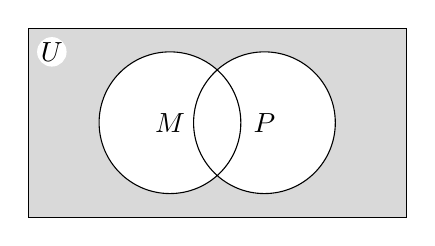
\begin{tikzpicture}[scale = 0.6]
        \filldraw [gray!30] (-3,-2) rectangle (5,2);
        \filldraw [white] (-2.5,1.5) circle (0.3);
        \draw (-2.5,1.5) node {$U$};
        \filldraw [white] (0,0) circle (1.5);
        \filldraw [white] (2,0) circle (1.5);
        \draw (0,0) circle (1.5) node {$M$} (2,0) circle (1.5) node {$P$};
        \draw (-3,-2) rectangle (5,2);
    \end{tikzpicture}
\end{center}


关联目标:

暂未关联目标



标签: 第一单元

答案: 暂无答案

解答或提示: 暂无解答与提示

使用记录:

暂无使用记录


出处: 代数精编第一章集合与命题
\item { (004837)}已知全集$U=\{2,4,3-a^2\}$, 集合$P=\{2,a^2-a+2\}$, $\complement_UP=\{-1\}$, 则实数$a$的取值等于\blank{50}.


关联目标:

暂未关联目标



标签: 第一单元

答案: 暂无答案

解答或提示: 暂无解答与提示

使用记录:

暂无使用记录


出处: 代数精编第一章集合与命题
\item { (004838)}已知集合$A,B$都是全集$U=\{1,2,3,4\}$的子集, 若$\complement_UA\cap B=\{1\}$, $A\cap B=\{3\}$, $\complement_UA\cap \complement_UB=\{2\}$, 则$A=$\blank{50}, $B=$\blank{50}.


关联目标:

暂未关联目标



标签: 第一单元

答案: 暂无答案

解答或提示: 暂无解答与提示

使用记录:

暂无使用记录


出处: 代数精编第一章集合与命题
\item { (004839)}已知全集$U=\{2,3,a^2+2a-3\}$, $A=\{b,2\}$, $\complement_UA=\{5\}$, 求实数$a$和$b$.


关联目标:

暂未关联目标



标签: 第一单元

答案: 暂无答案

解答或提示: 暂无解答与提示

使用记录:

暂无使用记录


出处: 代数精编第一章集合与命题
\item { (004840)}已知全集$U=\{-4,-3,-2,-1,0,1,2,3,4\}$, 集合$A=\{-3,a^2,a+1\}$, $B=\{a-3,2a-1,a^2+1\}$, 其中$a\in \mathbf{R}$, 若$A\cap B=\{-3\}$, 求$\complement_U(A\cup B)$.


关联目标:

暂未关联目标



标签: 第一单元

答案: 暂无答案

解答或提示: 暂无解答与提示

使用记录:

暂无使用记录


出处: 代数精编第一章集合与命题
\item { (004841)}记全集$U=\{\text{三角形}\}$, $A=\{\text{锐角三角形}\}$, $B=\{\text{钝角三角形}\}$, $C=\{\text{直角三角形}\}$, $D=\{\text{斜三角形}\}$, 求$\complement_U(A\cup B)\cap \complement_U(C\cup D)$.


关联目标:

暂未关联目标



标签: 第一单元

答案: 暂无答案

解答或提示: 暂无解答与提示

使用记录:

暂无使用记录


出处: 代数精编第一章集合与命题
\item { (004842)}已知全集$U=\{\text{小于}10\text{的自然数}\}$, 其子集$A,B$满足$\complement_UA\cap \complement_UB=\{1,9\}$, $A\cap B=\{2\}$, $\complement_UA\cap B=\{4,6,8\}$, 求集合$A$和$B$.


关联目标:

暂未关联目标



标签: 第一单元

答案: 暂无答案

解答或提示: 暂无解答与提示

使用记录:

暂无使用记录


出处: 代数精编第一章集合与命题
\item { (004843)}下列语句哪些不是命题? 哪些是命题? 如果是命题, 那么它们是真命题还是假命题? 为什么?\\
(1) 你到过北京吗?\\
(2) 当$x=4$时, $2x<0$;\\
(3) 若$x\in \mathbf{R}$, 则方程$x^2-x+1=0$无实数根;\\
(4) $1+2=5$或$3\ge 3$;\\
(5) $x<-2$或$x>2$;\\


关联目标:

暂未关联目标



标签: 第一单元

答案: 暂无答案

解答或提示: 暂无解答与提示

使用记录:

暂无使用记录


出处: 代数精编第一章集合与命题
\item { (004845)}写出下列命题的否定式:\\
(1) 不论$k$取何实数, $x^2+x+k=0$必有实数根;\\
(2) 三角形中至多有一个钝角;\\
(3) 正$n(n\ge 3)$边形的$n$个内角全相等;\\
(4) 张三是科大或北大的学生;\\
(5) 如果$x^2-x-2=0$, 那么$x\ne -1$且$x\ne -2$.


关联目标:

暂未关联目标



标签: 第一单元

答案: 暂无答案

解答或提示: 暂无解答与提示

使用记录:

暂无使用记录


出处: 代数精编第一章集合与命题
\item { (004848)}已知命题$\alpha$: 方程$x^2+mx+1=0$有两个相异负实数根, 命题$\beta$: $4x^2+4(m-2)x+1=0$无实数根, 命题$\alpha,\beta$有且只有一个为真命题, 求实数$m$的取值范围.


关联目标:

暂未关联目标



标签: 第一单元

答案: 暂无答案

解答或提示: 暂无解答与提示

使用记录:

暂无使用记录


出处: 代数精编第一章集合与命题
\item { (004852)}$(x+y)(y+z)(z+x)=0$的含义是\bracket{20}.
\twoch{$x,y,z$中有两个零}{$x,y,z$两两互为相反数}{$x,y,z$中至少有一个零}{$x,y,z$中至少有两个互为相反数}


关联目标:

暂未关联目标



标签: 第一单元

答案: 暂无答案

解答或提示: 暂无解答与提示

使用记录:

暂无使用记录


出处: 代数精编第一章集合与命题
\item { (004860)}若$p:\dfrac 1{x^2-1}>0$, 则$\overline p$为\blank{50}.


关联目标:

暂未关联目标



标签: 第一单元

答案: 暂无答案

解答或提示: 暂无解答与提示

使用记录:

暂无使用记录


出处: 代数精编第一章集合与命题
\item { (004861)}已知命题$p:$存在$x\in \mathbf{R}$, 使得$x^2+2ax+a\le 0$, 若命题$p$是假命题, 则实数$a$的取值范围是\blank{50}.


关联目标:

暂未关联目标



标签: 第一单元

答案: 暂无答案

解答或提示: 暂无解答与提示

使用记录:

暂无使用记录


出处: 代数精编第一章集合与命题
\item { (004865)}已知$\alpha :|a-1|<2$, $\beta:$方程$x^2+(a+2)x+1=0(x\in \mathbf{R})$没有正根, 求实数$a$的取值范围, 使$\alpha,\beta$有且只有一个为真命题.


关联目标:

暂未关联目标



标签: 第一单元

答案: 暂无答案

解答或提示: 暂无解答与提示

使用记录:

暂无使用记录


出处: 代数精编第一章集合与命题
\item { (004866)}已知关于$x$的方程$(x^2-1)^2-|x^2-1|+k=0$. 判断下列命题的真假:\\
(1) 存在实数$k$, 使得方程恰有$2$个不同的实数根;\\
(2) 存在实数$k$, 使得方程恰有$4$个不同的实数根;\\
(3) 存在实数$k$, 使得方程恰有$5$个不同的实数根;\\
(4) 存在实数$k$, 使得方程恰有$8$个不同的实数根.


关联目标:

暂未关联目标



标签: 第一单元

答案: 暂无答案

解答或提示: 暂无解答与提示

使用记录:

暂无使用记录


出处: 代数精编第一章集合与命题
\item { (004867)}如果$a,b,c$都是实数, 那么``$ac<0$''是``关于$x$的方程$ax^2+bx+c=0$有一个正根和一个负根''的\bracket{20}.
\twoch{必要不充分条件}{充分不必要条件}{充要条件}{既不充分也不必要条件}


关联目标:

暂未关联目标



标签: 第一单元

答案: 暂无答案

解答或提示: 暂无解答与提示

使用记录:

暂无使用记录


出处: 代数精编第一章集合与命题
\item { (004868)}已知$p:1\le x\le 4$, $q:\dfrac 1{x^2-x-12}>0$, 试问: $p$是$\overline q$的什么条件? 请说明理由.


关联目标:

暂未关联目标



标签: 第一单元

答案: 暂无答案

解答或提示: 暂无解答与提示

使用记录:

暂无使用记录


出处: 代数精编第一章集合与命题
\item { (004869)}设$\alpha ,\beta$是方程$x^2-ax+b=0$的两个实数根, 试分析``$a>2$且$b>1$''是``两根$\alpha ,\beta$均大于$1$''的什么条件.


关联目标:

暂未关联目标



标签: 第一单元

答案: 暂无答案

解答或提示: 暂无解答与提示

使用记录:

暂无使用记录


出处: 代数精编第一章集合与命题
\item { (004870)}已知$p:|x-3|\le 2$, $q:(x-m+1)(x-m-1)\le 0$, 若$\overline p$是$\overline q$的充分不必要条件, 求实数$m$的取值范围.


关联目标:

暂未关联目标



标签: 第一单元

答案: 暂无答案

解答或提示: 暂无解答与提示

使用记录:

暂无使用记录


出处: 代数精编第一章集合与命题
\item { (004871)}已知集合$A=\{x|x<-3\text{或}x>5\}$, $B=\{x|a\le x\le 8\}$.\\
(1) 求实数$a$的取值范围, 使它成为$A\cap B=\{x|5<x\le 8\}$的充要条件;\\
(2) 求实数$a$的一个值, 使它成为$A\cap B=\{x|5<x\le 8\}$的一个充分不必要条件;\\
(3) 求实数$a$的一个值, 使它成为$A\cap B=\{x|5<x\le 8\}$的一个必要不充分条件.


关联目标:

暂未关联目标



标签: 第一单元

答案: 暂无答案

解答或提示: 暂无解答与提示

使用记录:

暂无使用记录


出处: 代数精编第一章集合与命题
\item { (004872)}已知$a:0\le x<3$, $\beta:-1<x\le 4$, $\gamma:2x^2+mx-1<0$.\\
(1) 若$a$是$\gamma$的充分条件, 求实数$m$的取值范围;\\
(2) 若$\beta$是$\gamma$的充分条件, 求实数$m$的取值范围.


关联目标:

暂未关联目标



标签: 第一单元

答案: 暂无答案

解答或提示: 暂无解答与提示

使用记录:

暂无使用记录


出处: 代数精编第一章集合与命题
\item { (004874)}``$m=2$''是``函数$f(x)=x^2+mx-3$有两个零点''的\bracket{20}.
\twoch{充分不必要条件}{必要不充分条件}{充要条件}{既不充分也不必要条件}


关联目标:

暂未关联目标



标签: 第一单元

答案: 暂无答案

解答或提示: 暂无解答与提示

使用记录:

暂无使用记录


出处: 代数精编第一章集合与命题
\item { (004877)}``$\dfrac{x^2+x+1}{3x+2}<0$''是``$3x+2<0$''的\bracket{20}.
\twoch{充分不必要条件}{必要不充分条件}{充要条件}{既不充分也不必要条件}


关联目标:

暂未关联目标



标签: 第一单元

答案: 暂无答案

解答或提示: 暂无解答与提示

使用记录:

暂无使用记录


出处: 代数精编第一章集合与命题
\item { (004879)}已知$p:x^2+x-2>0$, $q:x>a$.若q是p的充分不必要条件, 则实数$a$的取值范围是\bracket{20}
\fourch{$a\ge 1$}{$a\ge 1$}{$a\ge -1$}{$a\le -3$}


关联目标:

暂未关联目标



标签: 第一单元

答案: 暂无答案

解答或提示: 暂无解答与提示

使用记录:

暂无使用记录


出处: 代数精编第一章集合与命题
\item { (004880)}方程$ax^2+2x+1=0$至少有一个负实数根的充要条件是\bracket{20}.
\fourch{$0<a\le 1$}{$a>1$}{$a\le 1$}{$0<a\le 1$或$a<0$}


关联目标:

暂未关联目标



标签: 第一单元

答案: 暂无答案

解答或提示: 暂无解答与提示

使用记录:

暂无使用记录


出处: 代数精编第一章集合与命题
\item { (004881)}若集合$A=\{-1,1\}$, $B=\{x|mx=1\}$, 且$B\subseteq A$, 则实数$m$的值为\bracket{20}.
\fourch{$1$}{$-1$}{$1$或$-1$}{$1$或$-1$或$0$}


关联目标:

暂未关联目标



标签: 第一单元

答案: 暂无答案

解答或提示: 暂无解答与提示

使用记录:

暂无使用记录


出处: 代数精编第一章集合与命题
\item { (004882)}给出下列命题: \textcircled{1} ``$x+y=0$''是``$x^2-y^2+x+y=0$''的充分不必要条件; \textcircled{2} ``$a-b<0$''是``$a^2-b^2<0$''的充分不必要条件; \textcircled{3} ``$a-b<0$''是``$a^2-b^2<0$''的必要不充分条件; \textcircled{4} ``两个三角形全等''是``两边和夹角对应相等''的充要条件.
其中属真命题的是\bracket{20}.
\fourch{\textcircled{1}\textcircled{2}}{\textcircled{1}\textcircled{3}}{\textcircled{2}\textcircled{3}}{\textcircled{1}\textcircled{4}}


关联目标:

暂未关联目标



标签: 第一单元

答案: 暂无答案

解答或提示: 暂无解答与提示

使用记录:

暂无使用记录


出处: 代数精编第一章集合与命题
\item { (004883)}有限集合$S$中元素的个数记作$\mathrm{card}(S)$, 设$A$, $B$都是有限集合, 给出下列命题:
\textcircled{1} $A\cap B=\varnothing$的充要条件是$\mathrm{card}(A\cup B)=\mathrm{card}(A)+\mathrm{card}(B)$; \textcircled{2} $A\subseteq B$的必要不充分条件是$\mathrm{card}(A)\le \mathrm{card}(B)$; \textcircled{3} $A\subseteq B$的充分不必要条件是$\mathrm{card}(A)\le \mathrm{card}(B)$; \textcircled{4} $A=B$的充要条件是$\mathrm{card}(A)=\mathrm{card}(B)$. 
其中真命题的个数是\bracket{20}.
\fourch{$0$}{$1$}{$2$}{$3$}


关联目标:

暂未关联目标



标签: 第一单元

答案: 暂无答案

解答或提示: 暂无解答与提示

使用记录:

暂无使用记录


出处: 代数精编第一章集合与命题
\item { (004884)}已知集合$A=\{-1,3,2m-1\}$, $B=\{3,m^2\}$, 若$B\subseteq A$, 则实数$m=$\blank{50}.


关联目标:

暂未关联目标



标签: 第一单元

答案: 暂无答案

解答或提示: 暂无解答与提示

使用记录:

暂无使用记录


出处: 代数精编第一章集合与命题
\item { (004885)}已知$p$是$r$的充分不必要条件, $s$是$r$的必要条件, $q$是$s$的必要条件, 那么$p$是$q$的\blank{50}条件.


关联目标:

暂未关联目标



标签: 第一单元

答案: 暂无答案

解答或提示: 暂无解答与提示

使用记录:

暂无使用记录


出处: 代数精编第一章集合与命题
\item { (004887)}``$xy>0$''的一个充分不必要条件是\blank{50}.


关联目标:

暂未关联目标



标签: 第一单元

答案: 暂无答案

解答或提示: 暂无解答与提示

使用记录:

暂无使用记录


出处: 代数精编第一章集合与命题
\item { (004888)}``$\sqrt x>\sqrt y$''的一个必要不充分条件是\blank{50}.


关联目标:

暂未关联目标



标签: 第一单元

答案: 暂无答案

解答或提示: 暂无解答与提示

使用记录:

暂无使用记录


出处: 代数精编第一章集合与命题
\item { (004889)}``$a^2+b^2>0$''的\blank{50}条件是``$a\ne 0$''.


关联目标:

暂未关联目标



标签: 第一单元

答案: 暂无答案

解答或提示: 暂无解答与提示

使用记录:

暂无使用记录


出处: 代数精编第一章集合与命题
\item { (004890)}若$p:x\ne 2$且$y\ne 3$, $q:x+y\ne 5$, 则是$p$是$q$成立的\blank{50}条件.


关联目标:

暂未关联目标



标签: 第一单元

答案: 暂无答案

解答或提示: 暂无解答与提示

使用记录:

暂无使用记录


出处: 代数精编第一章集合与命题
\item { (004891)}若集合$A=\{x|x^2+x-6=0\}$, $B=\{x|mx+1=0\}$, 则$B$是$A$的真子集的一个充分不必要条件是\blank{50}.


关联目标:

暂未关联目标



标签: 第一单元

答案: 暂无答案

解答或提示: 暂无解答与提示

使用记录:

暂无使用记录


出处: 代数精编第一章集合与命题
\item { (004892)}已知$p:\sqrt{x-1}>0$, $q:|x|=-x$, 试问: $p$是$\overline q$的什么条件? 请说明理由.


关联目标:

暂未关联目标



标签: 第一单元

答案: 暂无答案

解答或提示: 暂无解答与提示

使用记录:

暂无使用记录


出处: 代数精编第一章集合与命题
\item { (004893)}已知$m>0$, $p:-2\le x\le 10$, $q:1-m\le x\le -1+m$, 若$\overline p$是$\overline q$的必要不充分条件, 求实数$m$的取值范围.


关联目标:

暂未关联目标



标签: 第一单元

答案: 暂无答案

解答或提示: 暂无解答与提示

使用记录:

暂无使用记录


出处: 代数精编第一章集合与命题
\item { (004895)}设$x,y\in \mathbf{R}$, 求证: $|x+y|=|x|+|y|$成立的充要条件是$xy\ge 0$.


关联目标:

暂未关联目标



标签: 第一单元

答案: 暂无答案

解答或提示: 暂无解答与提示

使用记录:

暂无使用记录


出处: 代数精编第一章集合与命题
\item { (004896)}已知函数$f(x)=ax-bx^2$.\\
(1) 当$b>0$时, 若对任何$x\in \mathbf{R}$都有$f(x)\le 1$, 求证: $a\le 2\sqrt b$;\\
(2) 当$b>1$时, 求证: ``对任意$x\in [0,1]$, $|f(x)|\le 1$''的充要条件是$b-1\le a\le 2\sqrt b$.


关联目标:

暂未关联目标



标签: 第一单元

答案: 暂无答案

解答或提示: 暂无解答与提示

使用记录:

暂无使用记录


出处: 代数精编第一章集合与命题
\item { (004897)}当$a>b>0$时, 比较$\dfrac{2a+b}{a+2b}$和$\dfrac ab$的大小.


关联目标:

暂未关联目标



标签: 第一单元

答案: 暂无答案

解答或提示: 暂无解答与提示

使用记录:

暂无使用记录


出处: 代数精编第二章不等式
\item { (004898)}已知$a>0$, $a\ne 1$, $m>n>0$, 比较$A=a^m+\dfrac 1{a^m}$和$B=a^n+\dfrac 1{a^n}$的大小.


关联目标:

暂未关联目标



标签: 第一单元

答案: 暂无答案

解答或提示: 暂无解答与提示

使用记录:

暂无使用记录


出处: 代数精编第二章不等式
\item { (004899)}若$a>b$, 则下列各式中正确的是\bracket{20}.
\fourch{$a\lg x>b\lg x$($x>0$)}{$ax^2>bx^2$}{$a^2>b^2$}{$2^x\cdot a>2^x\cdot b$}


关联目标:

暂未关联目标



标签: 第一单元

答案: 暂无答案

解答或提示: 暂无解答与提示

使用记录:

暂无使用记录


出处: 代数精编第二章不等式
\item { (004900)}下列命题中, 不正确的一个是\bracket{20}.
\twoch{若$\sqrt[3]a>\sqrt[3]b$, 则$a>b$}{若$a>b$, $c>d$, 则$a-d>b-c$}{若$a>b>0$, $c>d>0$, 则$\dfrac ad>\dfrac bc$}{若$a>b>0$, $ac>bd$, 则$c>d$}


关联目标:

暂未关联目标



标签: 第一单元

答案: 暂无答案

解答或提示: 暂无解答与提示

使用记录:

暂无使用记录


出处: 代数精编第二章不等式
\item { (004901)}若$x<y<0$, 则有\bracket{20}.
\fourch{$0<x^2<xy$}{$y^2<xy<x^2$}{$xy<y^2<x^2$}{$y^2>x^2>0$}


关联目标:

暂未关联目标



标签: 第一单元

答案: 暂无答案

解答或提示: 暂无解答与提示

使用记录:

暂无使用记录


出处: 代数精编第二章不等式
\item { (004902)}若$a=\log_{0.2}0.3$, $b=\log_{0.3}0.2$, $c=1$, 则$a,b,c$的大小关系是\bracket{20}.
\fourch{$a>b>c$}{$b>a>c$}{$b>c>a$}{$c>b>a$}


关联目标:

暂未关联目标



标签: 第一单元|第二单元

答案: 暂无答案

解答或提示: 暂无解答与提示

使用记录:

暂无使用记录


出处: 代数精编第二章不等式
\item { (004903)}用不等号(``$>$''或``$<$'')填空:\\
(1) 若$a\ne b$, 则$a^2+3b^2$\blank{50}$2b(a+b)$;\\
(2) 若$c>1$, 则$\sqrt{c+1}-\sqrt c$\blank{50}$\sqrt c-\sqrt{c-1}$;\\
(3) 若$a>b$, $c>d$, 且$a$与$d$都是负数, 则$ac$\blank{50}$bd$.


关联目标:

暂未关联目标



标签: 第一单元

答案: 暂无答案

解答或提示: 暂无解答与提示

使用记录:

暂无使用记录


出处: 代数精编第二章不等式
\item { (004904)}若``$a>b$, $a-\dfrac 1a>b-\dfrac 1b$''同时成立, 则$ab$应满足的条件是\blank{50}.


关联目标:

暂未关联目标



标签: 第一单元

答案: 暂无答案

解答或提示: 暂无解答与提示

使用记录:

暂无使用记录


出处: 代数精编第二章不等式
\item { (004905)}已知$a>0$, $b>0$, 且$a\ne b$, 比较$\dfrac{a^2}b+\dfrac{b^2}a$与$a+b$的大小.


关联目标:

暂未关联目标



标签: 第一单元

答案: 暂无答案

解答或提示: 暂无解答与提示

使用记录:

暂无使用记录


出处: 代数精编第二章不等式
\item { (004906)}已知$0<\dfrac ab<\dfrac cd$, 比较$\dfrac b{a+b}$与$\dfrac d{c+d}$的大小.


关联目标:

暂未关联目标



标签: 第一单元

答案: 暂无答案

解答或提示: 暂无解答与提示

使用记录:

暂无使用记录


出处: 代数精编第二章不等式
\item { (004907)}若$x>y>1$, $0<a<1$, 则下列各式中正确的一个是\bracket{20}.
\fourch{${x^{-a}}>{y^{-a}}$}{$(\sin a)^x>(\sin a)^y$}{$\log_{\frac 1a}x<\log_{\frac 1a}y$}{$1+a^{x+y}>a^x+a^y$}


关联目标:

暂未关联目标



标签: 第一单元|第二单元|第三单元

答案: 暂无答案

解答或提示: 暂无解答与提示

使用记录:

暂无使用记录


出处: 代数精编第二章不等式
\item { (004908)}已知$a\in \mathbf{R}$, 比较$\dfrac 1{1+a}$与$1-a$的大小.


关联目标:

暂未关联目标



标签: 第一单元

答案: 暂无答案

解答或提示: 暂无解答与提示

使用记录:

暂无使用记录


出处: 代数精编第二章不等式
\item { (004909)}设$a>0$, $a\ne 1$, $t>0$, 比较$\dfrac 12\log_at$和$\log_a\dfrac{t+1}2$的大小.


关联目标:

暂未关联目标



标签: 第一单元|第二单元

答案: 暂无答案

解答或提示: 暂无解答与提示

使用记录:

暂无使用记录


出处: 代数精编第二章不等式
\item { (004910)}已知$x>y>0$, 比较$\sqrt{\dfrac{y^2+1}{x^2+1}}$与$\dfrac yx$的大小.


关联目标:

暂未关联目标



标签: 第一单元

答案: 暂无答案

解答或提示: 暂无解答与提示

使用记录:

暂无使用记录


出处: 代数精编第二章不等式
\item { (004911)}已知$a$, $b$, $m$, $n$都是正实数, 且$m+n=1$, 比较$\sqrt{ma+nb}$和$m\sqrt a+n\sqrt b$的大小.


关联目标:

暂未关联目标



标签: 第一单元

答案: 暂无答案

解答或提示: 暂无解答与提示

使用记录:

暂无使用记录


出处: 代数精编第二章不等式
\item { (004912)}解下列不等式:\\
(1) $6x^2-5x-1>0$;\\
(2) $6x^2-5x-1<0$;\\
(3) $5x^2-2x+3>0$;\\
(4) $9x^2+6x+1>0$;\\
(5) $3x^2-4x+5<0$.


关联目标:

暂未关联目标



标签: 第一单元

答案: 暂无答案

解答或提示: 暂无解答与提示

使用记录:

暂无使用记录


出处: 代数精编第二章不等式
\item { (004913)}已知关于$x$的不等式$ax^2+bx+c<0$的解集是$\{x|x<-2\text{或}x>-\dfrac 12\}$, 求$ax^2-bx+c>0$的解集.


关联目标:

暂未关联目标



标签: 第一单元

答案: 暂无答案

解答或提示: 暂无解答与提示

使用记录:

暂无使用记录


出处: 代数精编第二章不等式
\item { (004914)}已知集合$A=\{x|x^2+(a-1)x-a>0\}$, $B=\{x|(x+a)(x+b)>0\}$, $a\ne b$, $M=\{x|x^2-2x-3\le 0\}$.\\
(1) 若$\complement_UB=M$, 求$a$, $b$的值;\\
(2) 若$-1<b<a<1$, 求$A\cap B$;\\
(3) 若$-3<a<-1$, 且$a^2-1\in \complement_UA$, 求实数$a$的取值范围.


关联目标:

暂未关联目标



标签: 第一单元

答案: 暂无答案

解答或提示: 暂无解答与提示

使用记录:

暂无使用记录


出处: 代数精编第二章不等式
\item { (004915)}已知函数$y=(k^2+4k-5)x^2+4(1-k)x+3$的图象都在$x$轴的上方, 求实数$k$的取值范围.


关联目标:

暂未关联目标



标签: 第一单元

答案: 暂无答案

解答或提示: 暂无解答与提示

使用记录:

暂无使用记录


出处: 代数精编第二章不等式
\item { (004916)}已知$a<b$, 则下列各式中恒成立的是\bracket{20}.
\fourch{$a^2<b^2$}{$c-a>c-b$}{$|a|<|b|$}{$a-1>b-2$}


关联目标:

暂未关联目标



标签: 第一单元

答案: 暂无答案

解答或提示: 暂无解答与提示

使用记录:

暂无使用记录


出处: 代数精编第二章不等式
\item { (004917)}若$|x|>2$, 则\bracket{20}.
\fourch{$x>2$}{$x>\pm 2$}{$-2<x<2$}{$x>2$或$x<-2$}


关联目标:

暂未关联目标



标签: 第一单元

答案: 暂无答案

解答或提示: 暂无解答与提示

使用记录:

暂无使用记录


出处: 代数精编第二章不等式
\item { (004918)}不等式$|x|-3<0$的解集是\bracket{20}.
\fourch{$\{x|x<\pm 3\}$}{$\{x|-3<x<3\}$}{$\{x|x>3\}$}{$\{x|x<-3\}$}


关联目标:

暂未关联目标



标签: 第一单元

答案: 暂无答案

解答或提示: 暂无解答与提示

使用记录:

暂无使用记录


出处: 代数精编第二章不等式
\item { (004919)}已知集合$M=\{x||x|>2\},N=\{x|x<3\}$, 则下列结论正确的是\bracket{20}.
\twoch{$M\cup N=M$}{$M\cap N=\{x|2<x<3\}$}{$M\cup N=R$}{$M\cap N=\{x|x<-2\}$}


关联目标:

暂未关联目标



标签: 第一单元

答案: 暂无答案

解答或提示: 暂无解答与提示

使用记录:

暂无使用记录


出处: 代数精编第二章不等式
\item { (004920)}已知集合$M=\{x||x+1|\le 2\},P=\{x|x\le 2$或$x\ge 3\}$, 则$M$, $P$之间的关系是\bracket{20}.
\fourch{$M\supseteq P$}{$M\supset P$}{$M\subseteq P$}{$M\subset P$}


关联目标:

暂未关联目标



标签: 第一单元

答案: 暂无答案

解答或提示: 暂无解答与提示

使用记录:

暂无使用记录


出处: 代数精编第二章不等式
\item { (004921)}已知$|1-x|+\sqrt{x^2-4x+4}=1$, 则$x$的取值范围是\bracket{20}.
\fourch{$1\le x\le 2$}{$x\le 1$}{$x<1$或$x>2$}{$x\ge 2$}


关联目标:

暂未关联目标



标签: 第一单元

答案: 暂无答案

解答或提示: 暂无解答与提示

使用记录:

暂无使用记录


出处: 代数精编第二章不等式
\item { (004922)}不等式$2x+3-x^2>0$的解集是\bracket{20}.
\fourch{$\{x|-\dfrac 32\le x<1\}$}{$\{x|-1<x<3\}$}{$\{x|1\le x<3\}$}{$\{x|-\dfrac 32\le x<3\}$}


关联目标:

暂未关联目标



标签: 第一单元

答案: 暂无答案

解答或提示: 暂无解答与提示

使用记录:

暂无使用记录


出处: 代数精编第二章不等式
\item { (004923)}不等式$6x^2+5x<4$的解集是\bracket{20}.
\fourch{$\{x|x<-\dfrac 43\text{或}x>\dfrac 12\}$}{$\{x|-\dfrac 43<x<\dfrac 12\}.$}{$\{x|-\dfrac 12<x<\dfrac 43\}.$}{$\{x|x<-\dfrac 12\text{或}x>\dfrac 43\}$}


关联目标:

暂未关联目标



标签: 第一单元

答案: 暂无答案

解答或提示: 暂无解答与提示

使用记录:

暂无使用记录


出处: 代数精编第二章不等式
\item { (004924)}当$a<0$时, 关于$x$的不等式$x^2-4ax-5a^2>0$的解集是\bracket{20}.
\fourch{$\{x|x>5a\text{或}x<-a\}$}{$\{x|x<5a\text{或}x>-a\}$}{$\{x|-a<x<5a\}$}{$\{x|5a<x<-a\}$}


关联目标:

暂未关联目标



标签: 第一单元

答案: 暂无答案

解答或提示: 暂无解答与提示

使用记录:

暂无使用记录


出处: 代数精编第二章不等式
\item { (004925)}若$x$为实数, 则下列命题正确的是\bracket{20}.
\onech{$x^2\ge 2$的解集是$\{x|x\ge \pm \sqrt 2\}$}{$(x-1)^2<2$的解集是$\{x|1-\sqrt 2<x<1+\sqrt 2\}$}{$x^2-9<0$的解集是$\{x|x<3\}$}{设$x_1,x_2$为$ax^2+bx+c=0$的两个实根, 且$x_1>x_2$, 则$ax^2+bx+c>0$的解集是$\{x|x_2<x<x_1\}$}


关联目标:

暂未关联目标



标签: 第一单元

答案: 暂无答案

解答或提示: 暂无解答与提示

使用记录:

暂无使用记录


出处: 代数精编第二章不等式
\item { (004926)}在\textcircled{1} $x^2-2x-3<0$与$\dfrac{x^2-2x}{x-1}<\dfrac 3{x-1}$; \textcircled{2} $x^2+3x-4>0$与$x^2+3x+\sqrt x>4+\sqrt x$; \textcircled{3} $\dfrac{(x+2)(x^2-1)}{x+2}>0$与$x^2-1>0$''三组不等式中, 解集相同的组数是\bracket{20}.
\fourch{$0$}{$1$}{$2$}{$3$}


关联目标:

暂未关联目标



标签: 第一单元

答案: 暂无答案

解答或提示: 暂无解答与提示

使用记录:

暂无使用记录


出处: 代数精编第二章不等式
\item { (004927)}若$x^2+x<0$, 则$x^2,x,-x^2,-x$的大小关系是\bracket{20}.
\fourch{$x^2>x>-x^2>-x$}{$-x>x^2>-x^2>x$}{$-x>x^2>x>-x^2$}{$x^2>-x>x>-x^2$}


关联目标:

暂未关联目标



标签: 第一单元

答案: 暂无答案

解答或提示: 暂无解答与提示

使用记录:

暂无使用记录


出处: 代数精编第二章不等式
\item { (004928)}直接写出下列不等式的解集:\\
(1) $(x-1)^2>0$:\blank{50};\\
(2) $(2-x)(3x+1)>0$:\blank{50};\\
(3) $1-3x^2>2x$:\blank{50};\\
(4) $1-2x-x^2\ge 0$:\blank{50};\\
(5) $x+\sqrt x-6<0$:\blank{50}.


关联目标:

暂未关联目标



标签: 第一单元

答案: 暂无答案

解答或提示: 暂无解答与提示

使用记录:

暂无使用记录


出处: 代数精编第二章不等式
\item { (004929)}直接写出下列不等式的解集:\\
(1) $\dfrac{3x+4}{x-2}\ge 0$:\blank{50};\\
(2) $\dfrac{4-2x}{1+3x}>0$:\blank{50};\\
(3) $\dfrac 1x>x$:\blank{50};\\	
(4) $x^2-2|x|-3>0$:\blank{50};\\
(5) $x^2-x-5>|2x-1|$:\blank{50}.


关联目标:

暂未关联目标



标签: 第一单元

答案: 暂无答案

解答或提示: 暂无解答与提示

使用记录:

暂无使用记录


出处: 代数精编第二章不等式
\item { (004930)}若$\sqrt{x^2-x-6}\in \mathbf{R}$, 则$x$的取值范围为\blank{50}.


关联目标:

暂未关联目标



标签: 第一单元

答案: 暂无答案

解答或提示: 暂无解答与提示

使用记录:

暂无使用记录


出处: 代数精编第二章不等式
\item { (004931)}要使代数式$\dfrac{\sqrt{x-3}}{\sqrt{x^2-3x+2}}$有意义, 实数$x$的取值范围是\blank{50}.


关联目标:

暂未关联目标



标签: 第一单元

答案: 暂无答案

解答或提示: 暂无解答与提示

使用记录:

暂无使用记录


出处: 代数精编第二章不等式
\item { (004932)}若代数式$6x^2+x-2$的值恒取非负实数, 则实数$x$的取值范围是\blank{50}.


关联目标:

暂未关联目标



标签: 第一单元

答案: 暂无答案

解答或提示: 暂无解答与提示

使用记录:

暂无使用记录


出处: 代数精编第二章不等式
\item { (004933)}不等式$4\le x^2-3x<18$的整数解集是\blank{50}.


关联目标:

暂未关联目标



标签: 第一单元

答案: 暂无答案

解答或提示: 暂无解答与提示

使用记录:

暂无使用记录


出处: 代数精编第二章不等式
\item { (004934)}已知实数$x$满足$4x^2-4x-15\le 0$, 化简$\sqrt{x^2-8x+16}-|x-3|$.


关联目标:

暂未关联目标



标签: 第一单元

答案: 暂无答案

解答或提示: 暂无解答与提示

使用记录:

暂无使用记录


出处: 代数精编第二章不等式
\item { (004935)}已知$a>b$, 直接写出下列不等式的解集:\\
(1) $\dfrac{x-a}{x-b}\ge 0$:\blank{50};\\
(2) $\dfrac{x-a}{x-b}<0$:\blank{50};\\
(3) $x^2-(a-b)x+ab>0$:\blank{50};\\
(4) $x^2-(a-b)x+ab<0$:\blank{50}.


关联目标:

暂未关联目标



标签: 第一单元

答案: 暂无答案

解答或提示: 暂无解答与提示

使用记录:

暂无使用记录


出处: 代数精编第二章不等式
\item { (004936)}若关于$x$的方程$2kx^2+(8k+1)x+8k=0$有两个不等实根, 则实数$k$的取值范围是\blank{50}.


关联目标:

暂未关联目标



标签: 第一单元

答案: 暂无答案

解答或提示: 暂无解答与提示

使用记录:

暂无使用记录


出处: 代数精编第二章不等式
\item { (004937)}已知$a\ne 0$, 若关于$x$的不等式$ax^2-2ax+2a+3>0$无实数解, 则$a$的取值范围是\blank{50}.


关联目标:

暂未关联目标



标签: 第一单元

答案: 暂无答案

解答或提示: 暂无解答与提示

使用记录:

暂无使用记录


出处: 代数精编第二章不等式
\item { (004938)}不等式$\dfrac{x-1}{2x}\le 1$的解集是\bracket{20}.
\fourch{$\{x|x\ge -1\}$	}{$\{x|x\le -1\}$}{$\{x|-1\le x<0\}$}{$\{x|x\le -1\text{或}x>0\}$}


关联目标:

暂未关联目标



标签: 第一单元

答案: 暂无答案

解答或提示: 暂无解答与提示

使用记录:

暂无使用记录


出处: 代数精编第二章不等式
\item { (004939)}若关于$x$的二次不等式$mx^2+8mx+21<0$的解集是$\{x|-1<x<-1\}$, 则实数$m$的值等于\bracket{20}.
\fourch{$1$}{$2$}{$3$}{$4$}


关联目标:

暂未关联目标



标签: 第一单元

答案: 暂无答案

解答或提示: 暂无解答与提示

使用记录:

暂无使用记录


出处: 代数精编第二章不等式
\item { (004940)}若关于$x$的不等式$(a^2-3)x^2+5x-2>0$的解集是$\{x|\dfrac 12<x<2\}$, 则实数$a$的值等于\bracket{20}.
\fourch{$1$}{$-1$}{$\pm 1$}{$0$}


关联目标:

暂未关联目标



标签: 第一单元

答案: 暂无答案

解答或提示: 暂无解答与提示

使用记录:

暂无使用记录


出处: 代数精编第二章不等式
\item { (004941)}若关于$x$的不等式$ax^2+bx+c<0(a\ne 0)$的解集是空集, 则\bracket{20}.
\fourch{$a<0$且$b^2-4ac>0$}{$a<0$且$b^2-4ac\le 0$}{$a>0$且$b^2-4ac\le 0$}{$a>0$且$b^2-4ac>0$}


关联目标:

暂未关联目标



标签: 第一单元

答案: 暂无答案

解答或提示: 暂无解答与提示

使用记录:

暂无使用记录


出处: 代数精编第二章不等式
\item { (004942)}若对任何实数$x$, 二次函数$y=ax^2-x+c$的值恒为负, 则$a,c$应满足\bracket{20}.
\fourch{$\begin{cases}
   a>0,  \\ ac\le \dfrac 14  \end{cases}$}{$\begin{cases}
   a<0,  \\ ac<\dfrac 14  \end{cases}$}{$\begin{cases}
   a<0,  \\ ac>\dfrac 14  \end{cases}$}{$\begin{cases}
   a<0,  \\ ac<0  \end{cases}$}


关联目标:

暂未关联目标



标签: 第一单元

答案: 暂无答案

解答或提示: 暂无解答与提示

使用记录:

暂无使用记录


出处: 代数精编第二章不等式
\item { (004943)}若对任意实数$x$, 不等式$x^2+2(1+k)x+3+k>0$恒成立, 则$k$的取值范围是\bracket{20}.
\fourch{$-1<k<2$}{$-1\le k\le 2$}{$-2<k<1$}{$-2\le k\le 1$}


关联目标:

暂未关联目标



标签: 第一单元

答案: 暂无答案

解答或提示: 暂无解答与提示

使用记录:

暂无使用记录


出处: 代数精编第二章不等式
\item { (004944)}若关于$x$的二次方程$2(k+1)x^2+4kx+3k-2=0$的两根同号, 则$k$的取值范围是\bracket{20}.
\twoch{$-2<k<1$}{$-2\le k<-1$或$\dfrac 23<k\le 1$}{$k<-1$或$k>\dfrac 23$}{$-2<k<1$或$\dfrac 23<k<1$}


关联目标:

暂未关联目标



标签: 第一单元

答案: 暂无答案

解答或提示: 暂无解答与提示

使用记录:

暂无使用记录


出处: 代数精编第二章不等式
\item { (004945)}已知关于$x$的方程$(m+3)x^2-4mx+2m-1=0$的两根异号, 且负根的绝对值比正根大, 那么实数$m$的取值范围是\bracket{20}.
\fourch{$-3<m<0$}{$0<m<3$}{$m<-3$或$m>0$}{$m<0$或$m>3$}


关联目标:

暂未关联目标



标签: 第一单元

答案: 暂无答案

解答或提示: 暂无解答与提示

使用记录:

暂无使用记录


出处: 代数精编第二章不等式
\item { (004946)}若$\alpha ,\beta$是关于$x$的方程$x^2-(k-2)x+k^2+3k+5=0$($k$为实数)的两个实根, 则${{\alpha }^2}+{{\beta }^2}$的最大值等于\bracket{20}.
\fourch{$19$}{$18$}{$\dfrac{50}9$}{$-6$}


关联目标:

暂未关联目标



标签: 第一单元

答案: 暂无答案

解答或提示: 暂无解答与提示

使用记录:

暂无使用记录


出处: 代数精编第二章不等式
\item { (004947)}不等式$(x-1)(x-2)(x-3)(x-4)>120$的解为\bracket{20}.
\fourch{$x>6$}{$x<-1$或$x>6$}{$x<-1$}{$-1<x<6$}


关联目标:

暂未关联目标



标签: 第一单元

答案: 暂无答案

解答或提示: 暂无解答与提示

使用记录:

暂无使用记录


出处: 代数精编第二章不等式
\item { (004948)}在三个关于$x$的方程$x^2-ax+4=0$, $x^2+(a-1)x+16=0$和$x^2+2ax+3a+10=0$中, 已知至少有一个方程有实根, 则实数$a$的取值范围是\bracket{20}.
\fourch{$-4\le a\le 4$}{$-2<a<4$}{$a\le -2$或$a\ge 4$}{$a<0$}


关联目标:

暂未关联目标



标签: 第一单元

答案: 暂无答案

解答或提示: 暂无解答与提示

使用记录:

暂无使用记录


出处: 代数精编第二章不等式
\item { (004949)}若关于$x$的二次方程$x^2-2mx+4x+2m^2-4m-2=0$有实根, 则其两根之积的最大值等于\blank{50}.


关联目标:

暂未关联目标



标签: 第一单元

答案: 暂无答案

解答或提示: 暂无解答与提示

使用记录:

暂无使用记录


出处: 代数精编第二章不等式
\item { (004950)}使关于$x$的方程$x^2-kx+2k-3=0$的两实根的平方和取最小值, 实数$k$的值等于\blank{50}.


关联目标:

暂未关联目标



标签: 第一单元

答案: 暂无答案

解答或提示: 暂无解答与提示

使用记录:

暂无使用记录


出处: 代数精编第二章不等式
\item { (004951)}若关于$x$的不等式$x^2-mx+n\le 0$的解集是$\{x|-5\le x\le 1\}$, 则实数$m=$\blank{50}, $n=$\blank{50}.


关联目标:

暂未关联目标



标签: 第一单元

答案: 暂无答案

解答或提示: 暂无解答与提示

使用记录:

暂无使用记录


出处: 代数精编第二章不等式
\item { (004952)}若关于$x$的不等式$ax^2+bx+1\ge 0$的解集是$\{x|-5\le x\le 1\}$, 则实数$a=$\blank{50}, $b=$\blank{50}.


关联目标:

暂未关联目标



标签: 第一单元

答案: 暂无答案

解答或提示: 暂无解答与提示

使用记录:

暂无使用记录


出处: 代数精编第二章不等式
\item { (004953)}若关于$x$的不等式$ax^2+bx+2>0$的解集是$\{x|-\dfrac 12<x<\dfrac 13\}$, 则实数$a=$\blank{50}, $b=$\blank{50}.


关联目标:

暂未关联目标



标签: 第一单元

答案: 暂无答案

解答或提示: 暂无解答与提示

使用记录:

暂无使用记录


出处: 代数精编第二章不等式
\item { (004954)}若关于$x$的不等式$ax^2+bx-6>0$的解集是$\{x|2<x<3\}$, 则实数$a=$\blank{50}, $b=$\blank{50}.


关联目标:

暂未关联目标



标签: 第一单元

答案: 暂无答案

解答或提示: 暂无解答与提示

使用记录:

暂无使用记录


出处: 代数精编第二章不等式
\item { (004955)}若关于$x$的不等式$(a+b)x+(2a-3b)<0$的解集是$\{x|x>3\}$, 则不等式$(a-3b)x+b-2a>0$的解集是\blank{50}.


关联目标:

暂未关联目标



标签: 第一单元

答案: 暂无答案

解答或提示: 暂无解答与提示

使用记录:

暂无使用记录


出处: 代数精编第二章不等式
\item { (004956)}若关于$x$的不等式$ax^2+bx+c<0$的解集是$\{x|x<-2\text{或}x>-\dfrac 12\}$, 则关于$x$的不等式$ax^2-bx+c>0$的解集是\blank{50}.


关联目标:

暂未关联目标



标签: 第一单元

答案: 暂无答案

解答或提示: 暂无解答与提示

使用记录:

暂无使用记录


出处: 代数精编第二章不等式
\item { (004957)}解不等式$x^4-2x^2+1>x^2-1$.


关联目标:

暂未关联目标



标签: 第一单元

答案: 暂无答案

解答或提示: 暂无解答与提示

使用记录:

暂无使用记录


出处: 代数精编第二章不等式
\item { (004958)}已知关于$x$的不等式$kx^2-2x+6k<0(k\ne 0)$.\\
(1) 若不等式的解集是$\{x|x<-3\text{或}x>-2\}$, 求实数$k$的值;\\
(2) 若不等式的解集是$\{x|x\ne \dfrac 1k\}$, 求实数$k$的值;\\
(3) 若不等式的解集是实数集, 求实数$k$的值.


关联目标:

暂未关联目标



标签: 第一单元

答案: 暂无答案

解答或提示: 暂无解答与提示

使用记录:

暂无使用记录


出处: 代数精编第二章不等式
\item { (004959)}已知关于$x$的方程$m(x-1)=3(x+2)$的解是正实数, 求实数$m$的取值范围.


关联目标:

暂未关联目标



标签: 第一单元

答案: 暂无答案

解答或提示: 暂无解答与提示

使用记录:

暂无使用记录


出处: 代数精编第二章不等式
\item { (004960)}已知关于$x$的方程$\dfrac 14x^2-kx+5k-6=0$无实数解, 求实数$k$的取值范围.


关联目标:

暂未关联目标



标签: 第一单元

答案: 暂无答案

解答或提示: 暂无解答与提示

使用记录:

暂无使用记录


出处: 代数精编第二章不等式
\item { (004961)}已知关于$x$的方程$kx^2-(3k-1)x+k=0$有两个正实数根, 求实数$k$的取值范围.


关联目标:

暂未关联目标



标签: 第一单元

答案: 暂无答案

解答或提示: 暂无解答与提示

使用记录:

暂无使用记录


出处: 代数精编第二章不等式
\item { (004962)}已知集合$M=\{x|x^2-7x+10\le 0\}$, $N=\{x|x^2-(2-m)x+5-m\le 0\}$, 且$N\subseteq M$, 求实数$m$的取值范围.


关联目标:

暂未关联目标



标签: 第一单元

答案: 暂无答案

解答或提示: 暂无解答与提示

使用记录:

暂无使用记录


出处: 代数精编第二章不等式
\item { (004963)}已知集合$A=\{x|x^2+4x+p<0\}$, $B=\{x|x^2-x-2>0\}$, 且$A\subseteq B$, 求实数$p$的取值范围.


关联目标:

暂未关联目标



标签: 第一单元

答案: 暂无答案

解答或提示: 暂无解答与提示

使用记录:

暂无使用记录


出处: 代数精编第二章不等式
\item { (004964)}已知集合$A=\{x|x^2+ax+1\le 0\}$, $B=\{x|x^2-3x+2\le 0\}$, 且$A\subseteq B$, 求实数$a$的取值范围.


关联目标:

暂未关联目标



标签: 第一单元

答案: 暂无答案

解答或提示: 暂无解答与提示

使用记录:

暂无使用记录


出处: 代数精编第二章不等式
\item { (004965)}已知集合$A=\{x|x^2-2x-3\le 0\}$, $B=\{x|x^2+px+q<0\}$, 且$A\cap B=\{x|-1\le x<2\}$, 求实数$p,q$的关系式及其取值范围.


关联目标:

暂未关联目标



标签: 第一单元

答案: 暂无答案

解答或提示: 暂无解答与提示

使用记录:

暂无使用记录


出处: 代数精编第二章不等式
\item { (004966)}已知集合$A=\{x|-2<x<-1\text{或}x>\dfrac 12\}$, $B=\{x|x^2+ax+b\le 0\}$, 且$A\cup B=\{x|x+2>0\}$, $A\cap B=\{x|\dfrac 12<x\le 3\}$, 求$a,b$的值.


关联目标:

暂未关联目标



标签: 第一单元

答案: 暂无答案

解答或提示: 暂无解答与提示

使用记录:

暂无使用记录


出处: 代数精编第二章不等式
\item { (004967)}要使代数式$mx^2+(m-1)x+(m-1)$的值恒为负值, 求实数$m$的取值范围.


关联目标:

暂未关联目标



标签: 第一单元

答案: 暂无答案

解答或提示: 暂无解答与提示

使用记录:

暂无使用记录


出处: 代数精编第二章不等式
\item { (004968)}已知关于$x$的不等式$(a^2-4)x^2+(a+2)x-1\ge 0$的解集是空集, 求实数$a$的取值范围.


关联目标:

暂未关联目标



标签: 第一单元

答案: 暂无答案

解答或提示: 暂无解答与提示

使用记录:

暂无使用记录


出处: 代数精编第二章不等式
\item { (004969)}若关于$x$的不等式$\dfrac{x^2-8x+20}{mx^2+2(m+1)x+9m+4}<0$的解集为$\mathbf{R}$, 求实数$m$的取值范围.


关联目标:

暂未关联目标



标签: 第一单元

答案: 暂无答案

解答或提示: 暂无解答与提示

使用记录:

暂无使用记录


出处: 代数精编第二章不等式
\item { (004970)}当$0^\circ <\varphi <90^\circ$时, 要使$\dfrac{x^2-6x+8}{x^2+2}=\sin \varphi$恒成立, 求实数$x$的取值范围.


关联目标:

暂未关联目标



标签: 第一单元

答案: 暂无答案

解答或提示: 暂无解答与提示

使用记录:

暂无使用记录


出处: 代数精编第二章不等式
\item { (004971)}既要使关于$x$的不等式$x^2+(m-\dfrac 12)x-\dfrac 7{16}\le 0$有实数解, 又要使关于$x$的方程$(2m+3)x^2+mx+\dfrac{m-2}4=0$有实数解, 求实数$m$的取值范围.


关联目标:

暂未关联目标



标签: 第一单元

答案: 暂无答案

解答或提示: 暂无解答与提示

使用记录:

暂无使用记录


出处: 代数精编第二章不等式
\item { (004972)}为长$80\text{cm}$、宽$60\text{cm}$的工作台做一块台布, 使台布的面积是台面面积的两倍以上, 并使台子四边垂下的长度相等, 问: 垂下的长度至少是多少(精确到$0.1\text{cm}$)?


关联目标:

暂未关联目标



标签: 第一单元

答案: 暂无答案

解答或提示: 暂无解答与提示

使用记录:

暂无使用记录


出处: 代数精编第二章不等式
\item { (004973)}已知非零实数$x,y,z$, 满足$x+y+z=xyz$, $x^2=yz$, 求证: $x^2\ge 3$.


关联目标:

暂未关联目标



标签: 第一单元

答案: 暂无答案

解答或提示: 暂无解答与提示

使用记录:

暂无使用记录


出处: 代数精编第二章不等式
\item { (004974)}已知$a+b\ge 0$, 求证: $a^3+b^3\ge a^2b+ab^2$.


关联目标:

暂未关联目标



标签: 第一单元

答案: 暂无答案

解答或提示: 暂无解答与提示

使用记录:

暂无使用记录


出处: 代数精编第二章不等式
\item { (004975)}设$a,b\in \mathbf{R}^+$, 且$a\ne b$, 求证: $a^ab^b>a^bb^a$.


关联目标:

暂未关联目标



标签: 第一单元|第二单元

答案: 暂无答案

解答或提示: 暂无解答与提示

使用记录:

暂无使用记录


出处: 代数精编第二章不等式
\item { (004976)}已知$a,b,c\in \mathbf{R}$, 求证: $a^2+b^2+c^2\ge ab+bc+ca$.


关联目标:

暂未关联目标



标签: 第一单元

答案: 暂无答案

解答或提示: 暂无解答与提示

使用记录:

暂无使用记录


出处: 代数精编第二章不等式
\item { (004977)}已知$a,b,c>0$, 求证:
(1) $(a+b)(\dfrac 1a+\dfrac 1b)\ge 4$;\\
(2) $(a+b+c)(\dfrac 1a+\dfrac 1b+\dfrac 1c)\ge 9$.


关联目标:

暂未关联目标



标签: 第一单元

答案: 暂无答案

解答或提示: 暂无解答与提示

使用记录:

暂无使用记录


出处: 代数精编第二章不等式
\item { (004978)}已知正数$a,b$满足$a+b=1$, 求证: $\sqrt{2a+1}+\sqrt{2b+1}\le 2\sqrt 2$.


关联目标:

暂未关联目标



标签: 第一单元

答案: 暂无答案

解答或提示: 暂无解答与提示

使用记录:

暂无使用记录


出处: 代数精编第二章不等式
\item { (004979)}已知$\alpha ,\beta \in (0,\dfrac{\pi}2)$, 且$\alpha \ne \beta$, 求证: $\tan \alpha +\tan \beta >2\tan \dfrac{\alpha +\beta}2$.


关联目标:

暂未关联目标



标签: 第一单元|第三单元

答案: 暂无答案

解答或提示: 暂无解答与提示

使用记录:

暂无使用记录


出处: 代数精编第二章不等式
\item { (004980)}记$f(x)=x^2+ax+b$, 求证: $|f(1)|,|f(2)|,|f(3)|$中至少有一个不小于$\dfrac 12$.


关联目标:

暂未关联目标



标签: 第一单元|第二单元

答案: 暂无答案

解答或提示: 暂无解答与提示

使用记录:

暂无使用记录


出处: 代数精编第二章不等式
\item { (004981)}已知$-1\le x\le 1$, $n\ge 2$, $n\in \mathbf{N}$, 求证: $(1-x)^n+(1+x)^n\le 2^n$.


关联目标:

暂未关联目标



标签: 第一单元|第二单元

答案: 暂无答案

解答或提示: 暂无解答与提示

使用记录:

暂无使用记录


出处: 代数精编第二章不等式
\item { (004982)}已知$x+2y+3z=12$, 求证: $x^2+2y^2+3z^2\ge 24$.


关联目标:

暂未关联目标



标签: 第一单元

答案: 暂无答案

解答或提示: 暂无解答与提示

使用记录:

暂无使用记录


出处: 代数精编第二章不等式
\item { (004983)}已知$a,b,c\in \mathbf{R}^+$, 求证: $a^3+b^3+c^3\ge 3abc$(当且仅当$a=b=c$时取等号).


关联目标:

暂未关联目标



标签: 第一单元

答案: 暂无答案

解答或提示: 暂无解答与提示

使用记录:

暂无使用记录


出处: 代数精编第二章不等式
\item { (004984)}已知$a>0$, 求证: $x+\dfrac 1x+\dfrac 1{x+\dfrac 1x}\ge \dfrac 52$.


关联目标:

暂未关联目标



标签: 第一单元

答案: 暂无答案

解答或提示: 暂无解答与提示

使用记录:

暂无使用记录


出处: 代数精编第二章不等式
\item { (004985)}已知实数$a,b,c$满足$a+b+c=0$和$abc=2$, 求证: $a,b,c$中至少有一个不小于2.


关联目标:

暂未关联目标



标签: 第一单元

答案: 暂无答案

解答或提示: 暂无解答与提示

使用记录:

暂无使用记录


出处: 代数精编第二章不等式
\item { (004986)}已知$0<a<1$, $0<b<1$, 求证: $\sqrt{a^2+b^2}+\sqrt{(a-1)^2+b^2}+\sqrt{a^2+(b-1)^2}+\sqrt{(a-1)^2+(b-1)^2}\ge 2\sqrt 2$.


关联目标:

暂未关联目标



标签: 第一单元

答案: 暂无答案

解答或提示: 暂无解答与提示

使用记录:

暂无使用记录


出处: 代数精编第二章不等式
\item { (004987)}已知实数$x,y,z$不全为零, 求证: $\sqrt{x^2+xy+y^2}+\sqrt{y^2+yz+z^2}+\sqrt{z^2+zx+x^2}>\dfrac 32(x+y+z)$.


关联目标:

暂未关联目标



标签: 第一单元

答案: 暂无答案

解答或提示: 暂无解答与提示

使用记录:

暂无使用记录


出处: 代数精编第二章不等式
\item { (004988)}已知$x\ge 0$, $y\ge 0$, 求证: $\dfrac 12(x+y)^2+\dfrac 14(x+y)\ge x\sqrt y+y\sqrt x$.


关联目标:

暂未关联目标



标签: 第一单元

答案: 暂无答案

解答或提示: 暂无解答与提示

使用记录:

暂无使用记录


出处: 代数精编第二章不等式
\item { (004989)}求证: $1+\dfrac 14+\dfrac 19+\dfrac 1{16}+\cdots +\dfrac 1{n^2}<\dfrac 74(n\in \mathbf{N}^*)$.


关联目标:

暂未关联目标



标签: 第一单元

答案: 暂无答案

解答或提示: 暂无解答与提示

使用记录:

暂无使用记录


出处: 代数精编第二章不等式
\item { (004990)}已知$x>0$, $y>0$, $a,b$是正常数, 且满足$\dfrac ax+\dfrac by=1$, 求证: $x+y\ge (\sqrt a+\sqrt b)^2$.


关联目标:

暂未关联目标



标签: 第一单元

答案: 暂无答案

解答或提示: 暂无解答与提示

使用记录:

暂无使用记录


出处: 代数精编第二章不等式
\item { (004991)}已知正数$a,b$满足$a^2b=1$, 求$a+b$的最小值.


关联目标:

暂未关联目标



标签: 第一单元

答案: 暂无答案

解答或提示: 暂无解答与提示

使用记录:

暂无使用记录


出处: 代数精编第二章不等式
\item { (004992)}求$\sin^2\alpha\cos^2\alpha +\dfrac 1{\sin^2\alpha \cos^2\alpha }$的最小值.


关联目标:

暂未关联目标



标签: 第一单元|第三单元

答案: 暂无答案

解答或提示: 暂无解答与提示

使用记录:

暂无使用记录


出处: 代数精编第二章不等式
\item { (004993)}已知直角三角形的周长为定值$l$, 求它面积的最大值.


关联目标:

暂未关联目标



标签: 第一单元

答案: 暂无答案

解答或提示: 暂无解答与提示

使用记录:

暂无使用记录


出处: 代数精编第二章不等式
\item { (004994)}已知圆柱的体积为定值$V$, 求圆柱全面积的最小值.


关联目标:

暂未关联目标



标签: 第一单元|第六单元

答案: 暂无答案

解答或提示: 暂无解答与提示

使用记录:

暂无使用记录


出处: 代数精编第二章不等式
\item { (004995)}从半径为$R$的圆形铁片里剪去一个扇形, 然后把剩下部分卷成一个圆锥形漏斗, 要使漏斗有最大容量, 剪去扇形的圆心角$\theta$应是多少弧度?


关联目标:

暂未关联目标



标签: 第一单元|第二单元

答案: 暂无答案

解答或提示: 暂无解答与提示

使用记录:

暂无使用记录


出处: 代数精编第二章不等式
\item { (004996)}在Rt$\triangle ABC$中, 已知$\angle C=90^\circ$, $\angle A,\angle B,\angle C$的对边$a,b,c$满足$a+b=cx$. 设$\triangle ABC$绕直线$AB$旋转一周所得的旋转体的侧面积为$S_1$, $\triangle ABC$的内切圆面积为$S_2$. 求:\\
(1) 函数$f(x)=\dfrac{S_1}{S_2}$的解析式和定义域;\\
(2) 函数$f(x)$的最小值.


关联目标:

暂未关联目标



标签: 第一单元|第六单元

答案: 暂无答案

解答或提示: 暂无解答与提示

使用记录:

暂无使用记录


出处: 代数精编第二章不等式
\item { (004997)}用比较法证明以下各题:\\
(1) 已知$a>0$, $b>0$, 求证: $\dfrac 1a+\dfrac 1b\ge \dfrac 2{\sqrt{ab}}$;\\
(2) 已知$a>0$, $b>0$, 求证: $\dfrac b{\sqrt a}+\dfrac a{\sqrt b}\ge \sqrt a+\sqrt b$;\\
(3) 已知$a>0$, $b>0$, 求证: ${a^2}+{b^2}\ge (a+b)\sqrt{ab}$;\\
(4) 已知$0<x<1$, 求证: $\dfrac{a^2}x+\dfrac{b^2}{1-x}\ge (a+b)^2$.


关联目标:

暂未关联目标



标签: 第一单元

答案: 暂无答案

解答或提示: 暂无解答与提示

使用记录:

暂无使用记录


出处: 代数精编第二章不等式
\item { (004998)}已知$a\ge 0$, $b\ge 0$, 求证: $a^3+b^3\ge a^2b+b^2a$.


关联目标:

暂未关联目标



标签: 第一单元

答案: 暂无答案

解答或提示: 暂无解答与提示

使用记录:

暂无使用记录


出处: 代数精编第二章不等式
\item { (004999)}已知$x\in \mathbf{R}^+$, $y\in \mathbf{R}^+$, $n\in \mathbf{N}$, 求证: $x^{n+1}+y^{n+1} \ge x^ny+xy^n$.


关联目标:

暂未关联目标



标签: 第一单元

答案: 暂无答案

解答或提示: 暂无解答与提示

使用记录:

暂无使用记录


出处: 代数精编第二章不等式
\item { (005000)}已知$a>0$, $b>0$, $c>0$, 求证: $a(b^2+c^2)+b(c^2+a^2)+c(a^2+b^2)\ge 6abc$.


关联目标:

暂未关联目标



标签: 第一单元

答案: 暂无答案

解答或提示: 暂无解答与提示

使用记录:

暂无使用记录


出处: 代数精编第二章不等式
\item { (005001)}求证: $a^5+b^5\ge \dfrac 12(a^3+b^3)(a^2+b^2)$($a>0$, $b>0$).


关联目标:

暂未关联目标



标签: 第一单元

答案: 暂无答案

解答或提示: 暂无解答与提示

使用记录:

暂无使用记录


出处: 代数精编第二章不等式
\item { (005002)}求证: $a^2+b^2+c^2\ge ab+bc+ca$($a,b,c$是实数).


关联目标:

暂未关联目标



标签: 第一单元

答案: 暂无答案

解答或提示: 暂无解答与提示

使用记录:

暂无使用记录


出处: 代数精编第二章不等式
\item { (005003)}已知$a>b>c$, 求证: $a^2b+b^2c+c^2a>ab^2+bc^2+ca^2$.


关联目标:

暂未关联目标



标签: 第一单元

答案: 暂无答案

解答或提示: 暂无解答与提示

使用记录:

暂无使用记录


出处: 代数精编第二章不等式
\item { (005004)}在$\triangle ABC$中, 记$a,b,c$分别是角$A,B,C$的对边, $S$是$\triangle ABC$的面积, 求证: ${c^2}-{a^2}-{b^2}+4ab\ge 4\sqrt 3S$.


关联目标:

暂未关联目标



标签: 第一单元

答案: 暂无答案

解答或提示: 暂无解答与提示

使用记录:

暂无使用记录


出处: 代数精编第二章不等式
\item { (005005)}设$a,b\in \mathbf{N}$, 则$\sqrt 2$在$\dfrac ba$与$\dfrac{2a+b}{a+b}$之间.


关联目标:

暂未关联目标



标签: 第一单元

答案: 暂无答案

解答或提示: 暂无解答与提示

使用记录:

暂无使用记录


出处: 代数精编第二章不等式
\item { (005006)}已知$a,b,c$都是正数, 求证: $a^{2a}b^{2b}\ge a^{b+c}b^{c+a}c^{a+b}$.


关联目标:

暂未关联目标



标签: 第一单元

答案: 暂无答案

解答或提示: 暂无解答与提示

使用记录:

暂无使用记录


出处: 代数精编第二章不等式
\item { (005007)}下列命题中, 正确的一个是\bracket{20}.
\twoch{若$a,b,c\in \mathbf{R}$, 且$a>b$, 则$ac^2>bc^2$}{若$a,b\in \mathbf{R}$, 且$a\cdot b\ne 0$, 则$\dfrac ab+\dfrac ba\ge 2$}{若$a,b\in \mathbf{R}$, 且$a>|b|$, 则$a^n>b^n$($n\in \mathbf{N}$)}{若$a>b$, $c<d$, 则$\dfrac ac>\dfrac bd$}


关联目标:

暂未关联目标



标签: 第一单元

答案: 暂无答案

解答或提示: 暂无解答与提示

使用记录:

暂无使用记录


出处: 代数精编第二章不等式
\item { (005008)}下列各式中, 对任何实数$x$都成立的一个是\bracket{20}.
\fourch{$\lg (x^2+1)\ge \lg 2x$}{$x^2+1>2x$}{$\dfrac 1{x^2+1}\le 1$}{. $x+\dfrac 1x\ge 2$}


关联目标:

暂未关联目标



标签: 第一单元|第二单元

答案: 暂无答案

解答或提示: 暂无解答与提示

使用记录:

暂无使用记录


出处: 代数精编第二章不等式
\item { (005009)}已知, $a,b\in \mathbf{R}$, 且$a,b\ne 0$, 则在\textcircled{1} $\dfrac{a^2+b^2}2\ge ab$; \textcircled{2} $\dfrac ba+\dfrac ab\ge 2$;  \textcircled{3} $ab\le (\dfrac{a+b}2)^2$; \textcircled{4} $(\dfrac{a+b}2)^2\le \dfrac{a^2+b^2}2$这四个式子中, 恒成立的个数是\bracket{20}.
\fourch{$1$}{$2$}{$3$}{$4$}


关联目标:

暂未关联目标



标签: 第一单元

答案: 暂无答案

解答或提示: 暂无解答与提示

使用记录:

暂无使用记录


出处: 代数精编第二章不等式
\item { (005010)}若$a>0$, $b>0$, $c>0$, $d>0$, 则$\dfrac ba+\dfrac ab$的最小值为\blank{50}, $\dfrac ba+\dfrac cb+\dfrac ac$的最小值为\blank{50}, $\dfrac{b+c}a+\dfrac{c+a}b+\dfrac{a+b}c$的最小值为\blank{50}, $(a+b)(\dfrac 1a+\dfrac 1b)$的最小值为\blank{50}, $(\dfrac ba+\dfrac dc)(\dfrac cb+\dfrac ad)$的最小值为\blank{50}.


关联目标:

暂未关联目标



标签: 第一单元

答案: 暂无答案

解答或提示: 暂无解答与提示

使用记录:

暂无使用记录


出处: 代数精编第二章不等式
\item { (005011)}若$x>0$, 则$x+\dfrac 1x$的最小值为\blank{50}; 若$x<0$, 则$(-x)+\dfrac 1{-x}$的最小值为\blank{50}, $x+\dfrac 1x$的最大值为\blank{50}.


关联目标:

暂未关联目标



标签: 第一单元

答案: 暂无答案

解答或提示: 暂无解答与提示

使用记录:

暂无使用记录


出处: 代数精编第二章不等式
\item { (005012)}若$a>1$, $b>1$, $c>1$, 则$\log_ab+\log_ba$的最小值为\blank{50}, $\log_ab+\log_bc+\log_ca$的最小值为\blank{50}.


关联目标:

暂未关联目标



标签: 第一单元|第二单元

答案: 暂无答案

解答或提示: 暂无解答与提示

使用记录:

暂无使用记录


出处: 代数精编第二章不等式
\item { (005013)}若$0<a<1$, $0<b<1$, 则$\log_ab+\log_ba$的最小值为\blank{50}.


关联目标:

暂未关联目标



标签: 第一单元|第二单元

答案: 暂无答案

解答或提示: 暂无解答与提示

使用记录:

暂无使用记录


出处: 代数精编第二章不等式
\item { (005014)}若$a>1$, $0<b<1$, 则$\log_ab+\log_ba$的最大值为\blank{50}.


关联目标:

暂未关联目标



标签: 第一单元|第二单元

答案: 暂无答案

解答或提示: 暂无解答与提示

使用记录:

暂无使用记录


出处: 代数精编第二章不等式
\item { (005015)}设$a,b$为正数, 且$a+b\le 4$, 则下列各式中, 一定正确的是\bracket{20}.
\fourch{$\dfrac 1a+\dfrac 1b\le \dfrac 14$}{$\dfrac 14\le \dfrac 1a+\dfrac 1b\le \dfrac 12$}{$\dfrac 12\le \dfrac 1a+\dfrac 1b\le 1$}{$\dfrac 1a+\dfrac 1b\ge 1$}


关联目标:

暂未关联目标



标签: 第一单元

答案: 暂无答案

解答或提示: 暂无解答与提示

使用记录:

暂无使用记录


出处: 代数精编第二章不等式
\item { (005016)}若$a,b,c$均大于1, 且$\log_ac\cdot \log_bc=4$, 则下列各式中, 一定正确的是\bracket{20}.
\fourch{$ac\ge b$}{$ab\ge c$}{$bc\ge a$}{$ab\le c$}


关联目标:

暂未关联目标



标签: 第一单元|第二单元

答案: 暂无答案

解答或提示: 暂无解答与提示

使用记录:

暂无使用记录


出处: 代数精编第二章不等式
\item { (005017)}若$a>0$, $b>0$, 且$a\ne b$, 则下列各式恒成立的是\bracket{20}.
\fourch{$\dfrac{2ab}{a+b}<\dfrac{a+b}2<\sqrt{ab}$}{$\sqrt{ab}<\dfrac{2ab}{a+b}<\dfrac{a+b}2$}{$\dfrac{2ab}{a+b}<\sqrt{ab}<\dfrac{a+b}2$}{$\sqrt{ab}<\dfrac{a+b}2<\dfrac{2ab}{a+b}$}


关联目标:

暂未关联目标



标签: 第一单元

答案: 暂无答案

解答或提示: 暂无解答与提示

使用记录:

暂无使用记录


出处: 代数精编第二章不等式
\item { (005018)}利用公式$a^2+b^2\ge 2ab$或$a+b\ge 2\sqrt{ab}$($a,b\ge 0$), 求证:
若$x>0$, $y>0$, 则$\sqrt{(1+x)(1+y)}\ge 1+\sqrt{xy}$.


关联目标:

暂未关联目标



标签: 第一单元

答案: 暂无答案

解答或提示: 暂无解答与提示

使用记录:

暂无使用记录


出处: 代数精编第二章不等式
\item { (005019)}利用公式$a^2+b^2\ge 2ab$或$a+b\ge 2\sqrt{ab}$($a,b\ge 0$), 求证: 若$a>0$, $b>0$, $c>0$, 则$ab(a+b)+bc(b+c)+ca(c+a)\ge 6abc$.


关联目标:

暂未关联目标



标签: 第一单元

答案: 暂无答案

解答或提示: 暂无解答与提示

使用记录:

暂无使用记录


出处: 代数精编第二章不等式
\item { (005020)}利用公式$a^2+b^2\ge 2ab$或$a+b\ge 2\sqrt{ab}$($a,b\ge 0$), 求证: 若$a>0$, $b>0$, 则$a+b+\dfrac 1{\sqrt{ab}}\ge 2\sqrt 2$.


关联目标:

暂未关联目标



标签: 第一单元

答案: 暂无答案

解答或提示: 暂无解答与提示

使用记录:

暂无使用记录


出处: 代数精编第二章不等式
\item { (005021)}利用公式$a^2+b^2\ge 2ab$或$a+b\ge 2\sqrt{ab}$($a,b\ge 0$), 求证: 若$m=x{{\cos }^2}\theta +y{{\sin }^2}\theta$, $n=x{{\sin }^2}\theta +y{{\cos }^2}\theta$, 则$mn\ge xy$.


关联目标:

暂未关联目标



标签: 第一单元|第三单元

答案: 暂无答案

解答或提示: 暂无解答与提示

使用记录:

暂无使用记录


出处: 代数精编第二章不等式
\item { (005022)}利用公式$a^2+b^2\ge 2ab$或$a+b\ge 2\sqrt{ab}$($a,b\ge 0$), 求证: 若$x+3y-1=0$, 则${2^x}+{8^y}\ge 2\sqrt 2$.


关联目标:

暂未关联目标



标签: 第一单元

答案: 暂无答案

解答或提示: 暂无解答与提示

使用记录:

暂无使用记录


出处: 代数精编第二章不等式
\item { (005023)}利用公式$a^2+b^2\ge 2ab$或$a+b\ge 2\sqrt{ab}$($a,b\ge 0$), 求证: $\log_{0.5}(\dfrac 1{4^a}+\dfrac 1{4^b})\le a+b-1$.


关联目标:

暂未关联目标



标签: 第一单元|第二单元

答案: 暂无答案

解答或提示: 暂无解答与提示

使用记录:

暂无使用记录


出处: 代数精编第二章不等式
\item { (005024)}已知$x>0$, $y>0$, $x+y=1$, 求证:\\
(1) $(1+\dfrac 1x)(1+\dfrac 1y)\ge 9$;\\
(2) $(\dfrac 1{x^2}-1)(\dfrac 1{y^2}-1)\ge 9$.


关联目标:

暂未关联目标



标签: 第一单元

答案: 暂无答案

解答或提示: 暂无解答与提示

使用记录:

暂无使用记录


出处: 代数精编第二章不等式
\item { (005025)}已知$a>0$, $b>0$, $c>0$, $a+b+c=1$, 求证: $(1-a)(1-b)(1-c)\ge 8abc$.


关联目标:

暂未关联目标



标签: 第一单元

答案: 暂无答案

解答或提示: 暂无解答与提示

使用记录:

暂无使用记录


出处: 代数精编第二章不等式
\item { (005026)}已知$a>0$, $b>0$, $c>0$, $a+b+c=1$, 求证: $(\dfrac 1a-1)(\dfrac 1b-1)(\dfrac 1c-1)\ge 8$.


关联目标:

暂未关联目标



标签: 第一单元

答案: 暂无答案

解答或提示: 暂无解答与提示

使用记录:

暂无使用记录


出处: 代数精编第二章不等式
\item { (005027)}已知$a>0$, $b>0$, $c>0$, $a+b+c=1$, 求证: $\dfrac 1a+\dfrac 1b+\dfrac 1c\ge 9$.


关联目标:

暂未关联目标



标签: 第一单元

答案: 暂无答案

解答或提示: 暂无解答与提示

使用记录:

暂无使用记录


出处: 代数精编第二章不等式
\item { (005028)}已知$a>0$, $b>0$, $c>0$, $a+b+c=1$, 求证: $\dfrac 1{abc}\ge 27$.


关联目标:

暂未关联目标



标签: 第一单元

答案: 暂无答案

解答或提示: 暂无解答与提示

使用记录:

暂无使用记录


出处: 代数精编第二章不等式
\item { (005029)}已知$a>0$, $b>0$, $c>0$, $a+b+c=1$, 求证: $(1+\dfrac 1a)(1+\dfrac 1b)(1+\dfrac 1c)\ge 64$.


关联目标:

暂未关联目标



标签: 第一单元

答案: 暂无答案

解答或提示: 暂无解答与提示

使用记录:

暂无使用记录


出处: 代数精编第二章不等式
\item { (005030)}利用公式$\dfrac{a+b+c}3\le \sqrt{\dfrac{a^2+b^2+c^2}3}$, 求证: $\sqrt{a^2}+{b^2}+\sqrt{b^2}+{c^2}+\sqrt{c^2}+{a^2}\ge \sqrt 2(a+b+c)$.


关联目标:

暂未关联目标



标签: 第一单元

答案: 暂无答案

解答或提示: 暂无解答与提示

使用记录:

暂无使用记录


出处: 代数精编第二章不等式
\item { (005031)}利用公式$\dfrac{a+b}2\le \sqrt{\dfrac{a^2+b^2}2}$, 求证: 若$a+b=1(a,b\ge 0)$, 则$\sqrt{2a+1}+\sqrt{2b+1}\le 2\sqrt 2$.


关联目标:

暂未关联目标



标签: 第一单元

答案: 暂无答案

解答或提示: 暂无解答与提示

使用记录:

暂无使用记录


出处: 代数精编第二章不等式
\item { (005032)}利用公式$\dfrac{a+b+c}3\le \sqrt{\dfrac{a^2+b^2+c^2}3}$, 求证: 若$a+b+c=1(a,b,c\ge 0)$, 则$\sqrt{13a+1}+\sqrt{13b+1}+\sqrt{13c+1}\le 4\sqrt 3$.


关联目标:

暂未关联目标



标签: 第一单元

答案: 暂无答案

解答或提示: 暂无解答与提示

使用记录:

暂无使用记录


出处: 代数精编第二章不等式
\item { (005033)}利用公式$\dfrac{a+b}2\le \sqrt{\dfrac{a^2+b^2}2}$, 求证: $a\cos \varphi +b\sin \varphi +c\le \sqrt{2(a^2+b^2+c^2)}$.


关联目标:

暂未关联目标



标签: 第一单元|第三单元

答案: 暂无答案

解答或提示: 暂无解答与提示

使用记录:

暂无使用记录


出处: 代数精编第二章不等式
\item { (005034)}利用$a^2+b^2+c^2\ge ab+bc+ca(a,b,c\in \mathbf{R})$, 证明: 若$a>0$, $b>0$, $c>0$, 则$\dfrac{a^2}{b^2}+{b^2}{c^2}+{c^2}{a^2}{a+b+c}\ge abc$.


关联目标:

暂未关联目标



标签: 第一单元

答案: 暂无答案

解答或提示: 暂无解答与提示

使用记录:

暂无使用记录


出处: 代数精编第二章不等式
\item { (005035)}利用$a^2+b^2+c^2\ge ab+bc+ca(a,b,c\in \mathbf{R})$, 证明: 若半径为$1$的圆内接$\triangle ABC$的而积为$\dfrac 14$, 二边长分别为$a,b,c$, 则\\(1) $abc=1$;\\
(2) $\sqrt b+\sqrt c<\dfrac 1a+\dfrac 1b+\dfrac 1c$.


关联目标:

暂未关联目标



标签: 第一单元

答案: 暂无答案

解答或提示: 暂无解答与提示

使用记录:

暂无使用记录


出处: 代数精编第二章不等式
\item { (005036)}利用$a^2+b^2+c^2\ge ab+bc+ca(a,b,c\in \mathbf{R})$, 证明: 若$a,b,c>0$, $n\in \mathbf{N}$, $f(n)=\lg \dfrac{a^n+b^n+c^n}3$, 则$2f(n)\le f(2n)$.


关联目标:

暂未关联目标



标签: 第一单元|第二单元

答案: 暂无答案

解答或提示: 暂无解答与提示

使用记录:

暂无使用记录


出处: 代数精编第二章不等式
\item { (005037)}利用放缩法并结合公式$ab\le (\dfrac{a+b}2)^2$, 证明: $\lg 9\cdot \lg 11<1$.


关联目标:

暂未关联目标



标签: 第一单元

答案: 暂无答案

解答或提示: 暂无解答与提示

使用记录:

暂无使用记录


出处: 代数精编第二章不等式
\item { (005038)}利用放缩法并结合公式$ab\le (\dfrac{a+b}2)^2$, 证明: $\log_a(a-1)\cdot \log_a(a+1)<1$($a>1$).


关联目标:

暂未关联目标



标签: 第一单元|第二单元

答案: 暂无答案

解答或提示: 暂无解答与提示

使用记录:

暂无使用记录


出处: 代数精编第二章不等式
\item { (005039)}利用放缩法并结合公式$ab\le (\dfrac{a+b}2)^2$, 证明: 若$a>b>c$, 则$\dfrac 1{a-b}+\dfrac 1{b-c}+\dfrac 4{c-a}\ge 0$.


关联目标:

暂未关联目标



标签: 第一单元

答案: 暂无答案

解答或提示: 暂无解答与提示

使用记录:

暂无使用记录


出处: 代数精编第二章不等式
\item { (005040)}利用放缩法证明: $\dfrac 1n+\dfrac 1{n+1}+\dfrac 1{n+2}+\dfrac 1{n+3}+\dfrac 1{n+4}+\cdots +\dfrac 1{n^2}>1$($n\in \mathbf{N}$, $n\ge 2$).


关联目标:

暂未关联目标



标签: 第一单元

答案: 暂无答案

解答或提示: 暂无解答与提示

使用记录:

暂无使用记录


出处: 代数精编第二章不等式
\item { (005041)}利用放缩法证明: $\dfrac 12\le \dfrac 1{n+1}+\dfrac 1{n+2}+\cdots +\dfrac 1{2n}<1$($n\in \mathbf{N}$).


关联目标:

暂未关联目标



标签: 第一单元

答案: 暂无答案

解答或提示: 暂无解答与提示

使用记录:

暂无使用记录


出处: 代数精编第二章不等式
\item { (005042)}利用放缩法证明: 已知$a>0$, $b>0$, $c>0$, 且$a^2+b^2=c^2$, 求证: $a^n+b^n<c^n$($n\ge 3$, $n\in \mathbf{N}$).


关联目标:

暂未关联目标



标签: 第一单元

答案: 暂无答案

解答或提示: 暂无解答与提示

使用记录:

暂无使用记录


出处: 代数精编第二章不等式
\item { (005043)}利用拆项法证明: 若$x>y$, $xy=1$, 则$\dfrac{x^2+y^2}{x-y}\ge 2\sqrt 2$.


关联目标:

暂未关联目标



标签: 第一单元

答案: 暂无答案

解答或提示: 暂无解答与提示

使用记录:

暂无使用记录


出处: 代数精编第二章不等式
\item { (005044)}利用拆项法证明: $\dfrac 12({a^2}+{b^2})+1\ge \sqrt{{a^2}+1}\cdot \sqrt{{b^2}+1}$.


关联目标:

暂未关联目标



标签: 第一单元

答案: 暂无答案

解答或提示: 暂无解答与提示

使用记录:

暂无使用记录


出处: 代数精编第二章不等式
\item { (005045)}利用拆项法证明: 若$a>0$, $b>0$, $c>0$, 则$2(\dfrac{a+b}2-\sqrt{ab})\le 3(\dfrac{a+b+c}3-\sqrt[3]{abc})$.


关联目标:

暂未关联目标



标签: 第一单元

答案: 暂无答案

解答或提示: 暂无解答与提示

使用记录:

暂无使用记录


出处: 代数精编第二章不等式
\item { (005046)}利用拆项法证明: $2(\sqrt{n+1}-1)<1+\dfrac 1{\sqrt 2}+\dfrac 1{\sqrt 3}+\cdots +\dfrac 1{\sqrt n}<2\sqrt n$($n\in \mathbf{N}$).


关联目标:

暂未关联目标



标签: 第一单元

答案: 暂无答案

解答或提示: 暂无解答与提示

使用记录:

暂无使用记录


出处: 代数精编第二章不等式
\item { (005047)}利用逆代法证明: 若正数$x,y$满足$x+2y=1$, 则$\dfrac 1x+\dfrac 1y\ge 3+2\sqrt 2$.


关联目标:

暂未关联目标



标签: 第一单元

答案: 暂无答案

解答或提示: 暂无解答与提示

使用记录:

暂无使用记录


出处: 代数精编第二章不等式
\item { (005048)}利用逆代法证明: $\dfrac 1{\sin ^2\alpha}+\dfrac 3{\cos^2\alpha}\ge 4+2\sqrt 3$.


关联目标:

暂未关联目标



标签: 第一单元|第三单元

答案: 暂无答案

解答或提示: 暂无解答与提示

使用记录:

暂无使用记录


出处: 代数精编第二章不等式
\item { (005049)}利用逆代法证明: 若$x,y>0$, $a,b$为正常数, 且$\dfrac ax+\dfrac ay=1$, 则$x+y\ge (\sqrt a+\sqrt b)^2$.


关联目标:

暂未关联目标



标签: 第一单元

答案: 暂无答案

解答或提示: 暂无解答与提示

使用记录:

暂无使用记录


出处: 代数精编第二章不等式
\item { (005050)}利用判别式法证明: $\dfrac 13\le \dfrac{x^2-x+1}{x^2+x+1}\le 3$.


关联目标:

暂未关联目标



标签: 第一单元

答案: 暂无答案

解答或提示: 暂无解答与提示

使用记录:

暂无使用记录


出处: 代数精编第二章不等式
\item { (005051)}利用判别式法证明: 若关于$x$的不等式$(a^2-1)x^2-(a-1)x-1<0(a\in \mathbf{R})$对仟意实数$x$恒成立, 则$-\dfrac 35<a\le 1$.


关联目标:

暂未关联目标



标签: 第一单元

答案: 暂无答案

解答或提示: 暂无解答与提示

使用记录:

暂无使用记录


出处: 代数精编第二章不等式
\item { (005052)}利用函数的单调性证明: 若$x>0$, $y>0$, $x+y=1$, 则$(x+\dfrac 1x)(y+\dfrac 1y)\ge \dfrac{25}4$.


关联目标:

暂未关联目标



标签: 第一单元|第二单元

答案: 暂无答案

解答或提示: 暂无解答与提示

使用记录:

暂无使用记录


出处: 代数精编第二章不等式
\item { (005053)}利用函数的单调性证明: 若$0<a<\dfrac 1k(k\ge 2,k\in \mathbf{N})$, 且$a^2<a-b$, 则$b<\dfrac 1{k+1}$.


关联目标:

暂未关联目标



标签: 第一单元|第二单元

答案: 暂无答案

解答或提示: 暂无解答与提示

使用记录:

暂无使用记录


出处: 代数精编第二章不等式
\item { (005054)}利用三角换元法证明: 若$a^2+b^2=1$, 则$a\sin x+b\cos x\le 1$.


关联目标:

暂未关联目标



标签: 第一单元|第三单元

答案: 暂无答案

解答或提示: 暂无解答与提示

使用记录:

暂无使用记录


出处: 代数精编第二章不等式
\item { (005055)}利用三角换元法证明: 若$|a|<1$, $|b|<1$, 则$|ab\pm \sqrt{(1-{a^2})(1-{b^2})}|\le 1$.


关联目标:

暂未关联目标



标签: 第一单元|第三单元

答案: 暂无答案

解答或提示: 暂无解答与提示

使用记录:

暂无使用记录


出处: 代数精编第二章不等式
\item { (005056)}利用三角换元法证明: 若$x^2+y^2\le 1$, 则$-\sqrt 2\le x^2+2xy-y^2\le \sqrt 2$.


关联目标:

暂未关联目标



标签: 第一单元|第三单元

答案: 暂无答案

解答或提示: 暂无解答与提示

使用记录:

暂无使用记录


出处: 代数精编第二章不等式
\item { (005057)}利用三角换元法证明: 若$|x|\le 1$, 则$(1+x)^n+(1-x)^n\le 2^n$.


关联目标:

暂未关联目标



标签: 第一单元|第三单元

答案: 暂无答案

解答或提示: 暂无解答与提示

使用记录:

暂无使用记录


出处: 代数精编第二章不等式
\item { (005058)}利用三角换元法证明: 若$a>0$, $b>0$, 且$a-b=1$, 则$0<\dfrac 1a(\sqrt a-\dfrac 1{\sqrt a})(\sqrt b+\dfrac 1{\sqrt b})<1$.


关联目标:

暂未关联目标



标签: 第一单元|第三单元

答案: 暂无答案

解答或提示: 暂无解答与提示

使用记录:

暂无使用记录


出处: 代数精编第二章不等式
\item { (005059)}利用三角换元法证明: $0<\sqrt{1+x}-\sqrt x\le 1$.


关联目标:

暂未关联目标



标签: 第一单元|第三单元

答案: 暂无答案

解答或提示: 暂无解答与提示

使用记录:

暂无使用记录


出处: 代数精编第二章不等式
\item { (005060)}试构造几何图形证明: 若$f(x)=\sqrt{1+x^2}$, $x>b>0$, 则$|f(a)-f(b)|<|a-b|$.


关联目标:

暂未关联目标



标签: 第一单元

答案: 暂无答案

解答或提示: 暂无解答与提示

使用记录:

暂无使用记录


出处: 代数精编第二章不等式
\item { (005061)}试构造几何图形证明: 若$x,y,z>0$, 则$\sqrt{x^2+y^2+xy}+\sqrt{y^2+z^2+yz}>\sqrt{z^2+x^2+zx}$.


关联目标:

暂未关联目标



标签: 第一单元

答案: 暂无答案

解答或提示: 暂无解答与提示

使用记录:

暂无使用记录


出处: 代数精编第二章不等式
\item { (005062)}利用均值换元证明: 若$a>0$, $b>0$, 且$a+b=1$, 则$\dfrac 43\le \dfrac 1{a+1}+\dfrac 1{b+1}<\dfrac 32$.


关联目标:

暂未关联目标



标签: 第一单元

答案: 暂无答案

解答或提示: 暂无解答与提示

使用记录:

暂无使用记录


出处: 代数精编第二章不等式
\item { (005063)}利用均值换元证明: 若$a+b+c=1$, 则${a^2}+{b^2}+{c^2}\ge \dfrac 13$.


关联目标:

暂未关联目标



标签: 第一单元

答案: 暂无答案

解答或提示: 暂无解答与提示

使用记录:

暂无使用记录


出处: 代数精编第二章不等式
\item { (005064)}利用设差换元证明: 若$x\ge y\ge 0$, 则$\sqrt{2xy-{y^2}}+\sqrt{x^2-y^2}\ge x$.


关联目标:

暂未关联目标



标签: 第一单元

答案: 暂无答案

解答或提示: 暂无解答与提示

使用记录:

暂无使用记录


出处: 代数精编第二章不等式
\item { (005065)}已知$a,b,c$都是正数, 求证: $a^ab^bc^c\ge (abc)^{\frac{a+b+c}3}$.


关联目标:

暂未关联目标



标签: 第一单元

答案: 暂无答案

解答或提示: 暂无解答与提示

使用记录:

暂无使用记录


出处: 代数精编第二章不等式
\item { (005066)}已知正数$a,b$满足$a+b=1$, 求证: $(ax+by)(ay+bx)\ge xy$.


关联目标:

暂未关联目标



标签: 第一单元

答案: 暂无答案

解答或提示: 暂无解答与提示

使用记录:

暂无使用记录


出处: 代数精编第二章不等式
\item { (005067)}已知正数$a,b$满足$a+b=1$, 求证: $(a+\dfrac 1a)^2+(b+\dfrac 1b)^2\ge \dfrac{25}2$.


关联目标:

暂未关联目标



标签: 第一单元

答案: 暂无答案

解答或提示: 暂无解答与提示

使用记录:

暂无使用记录


出处: 代数精编第二章不等式
\item { (005068)}已知正数$a,b$满足$a+b=1$, 求证: $(a+\dfrac 1a)(b+\dfrac 1b)\ge \dfrac{25}4$.


关联目标:

暂未关联目标



标签: 第一单元

答案: 暂无答案

解答或提示: 暂无解答与提示

使用记录:

暂无使用记录


出处: 代数精编第二章不等式
\item { (005069)}已知正数$a,b,c$满足$a+b+c=1$, 求证: $(a+\dfrac 1a)+(b+\dfrac 1b)+(c+\dfrac 1c)\ge 10$.


关联目标:

暂未关联目标



标签: 第一单元

答案: 暂无答案

解答或提示: 暂无解答与提示

使用记录:

暂无使用记录


出处: 代数精编第二章不等式
\item { (005070)}已知正数$a,b,c$满足$a+b+c=1$, 求证: $(a+\dfrac 1a)^2+(b+\dfrac 1b)^2+(c+\dfrac 1c)^2\ge \dfrac{100}3$


关联目标:

暂未关联目标



标签: 第一单元

答案: 暂无答案

解答或提示: 暂无解答与提示

使用记录:

暂无使用记录


出处: 代数精编第二章不等式
\item { (005071)}已知正数$a,b,c$满足$a+b+c=1$, 求证: $\dfrac 1{\sqrt a}+\dfrac 1{\sqrt b}+\dfrac 1{\sqrt c}\ge 3\sqrt 3$.


关联目标:

暂未关联目标



标签: 第一单元

答案: 暂无答案

解答或提示: 暂无解答与提示

使用记录:

暂无使用记录


出处: 代数精编第二章不等式
\item { (005072)}已知$a^2+b^2+c^2=1$, 求证: $-\dfrac 12\le ab+bc+ca\le 1$.


关联目标:

暂未关联目标



标签: 第一单元

答案: 暂无答案

解答或提示: 暂无解答与提示

使用记录:

暂无使用记录


出处: 代数精编第二章不等式
\item { (005073)}已知$a^2+b^2+c^2=1$, 求证: $|abc|\le \dfrac{\sqrt 3}9$.


关联目标:

暂未关联目标



标签: 第一单元

答案: 暂无答案

解答或提示: 暂无解答与提示

使用记录:

暂无使用记录


出处: 代数精编第二章不等式
\item { (005074)}已知$x>1$, 求证: $\sqrt x-\sqrt{x-1}>\sqrt{x+1}-\sqrt x$.


关联目标:

暂未关联目标



标签: 第一单元

答案: 暂无答案

解答或提示: 暂无解答与提示

使用记录:

暂无使用记录


出处: 代数精编第二章不等式
\item { (005075)}已知$a>0$, $b>0$, $c>0$, 求证: $\dfrac 1a+\dfrac 1b+\dfrac 1c\ge 2(\dfrac 1{a+b}+\dfrac 1{b+c}+\dfrac 1{c+a})$.


关联目标:

暂未关联目标



标签: 第一单元

答案: 暂无答案

解答或提示: 暂无解答与提示

使用记录:

暂无使用记录


出处: 代数精编第二章不等式
\item { (005076)}已知$a>0$, $b>0$, $c>0$, 求证: $\dfrac c{a+b}+\dfrac a{b+c}+\dfrac b{c+a}\ge \dfrac 32$.


关联目标:

暂未关联目标



标签: 第一单元

答案: 暂无答案

解答或提示: 暂无解答与提示

使用记录:

暂无使用记录


出处: 代数精编第二章不等式
\item { (005077)}已知$\alpha ,\beta \in (0,\dfrac{\pi}2)$, 求证: $\dfrac 1{\cos^2\alpha}+\dfrac 1{\sin^2\alpha \sin^2\beta\cos^2\beta}\ge 9$.


关联目标:

暂未关联目标



标签: 第一单元

答案: 暂无答案

解答或提示: 暂无解答与提示

使用记录:

暂无使用记录


出处: 代数精编第二章不等式
\item { (005078)}已知$a>0$, $b>0$, $c>0$, 求证: $\dfrac 1{a+b}+\dfrac 1{b+c}+\dfrac 1{c+a}\ge \dfrac 9{2(a+b+c)}$.


关联目标:

暂未关联目标



标签: 第一单元

答案: 暂无答案

解答或提示: 暂无解答与提示

使用记录:

暂无使用记录


出处: 代数精编第二章不等式
\item { (005079)}己知$\tan \alpha,\tan \beta$是关于$x$的方程$mx^2+(2m-3)x+(m-2)=0(m\ne 0)$的两根, 求证: $\tan (\alpha +\beta)\ge -\dfrac 34$.


关联目标:

暂未关联目标



标签: 第一单元|第三单元

答案: 暂无答案

解答或提示: 暂无解答与提示

使用记录:

暂无使用记录


出处: 代数精编第二章不等式
\item { (005080)}已知长方体的对角线长为定长$l$, 求证: 它的体积$V\le \dfrac{\sqrt 3l^3}9$.


关联目标:

暂未关联目标



标签: 第一单元

答案: 暂无答案

解答或提示: 暂无解答与提示

使用记录:

暂无使用记录


出处: 代数精编第二章不等式
\item { (005088)}求证: $\dfrac{x+b+c+abc}{1+ab+bc+ca}\le 1$, 其中$0\le a\le 1$, $0\le b\le 1$, $0\le c\le 1$.


关联目标:

暂未关联目标



标签: 第一单元

答案: 暂无答案

解答或提示: 暂无解答与提示

使用记录:

暂无使用记录


出处: 代数精编第二章不等式
\item { (005091)}求证: 若$a>b>0$, $c>d>0$, 则$\sqrt{ac}-\sqrt{bd}>\sqrt{(a-b)(c-d)}$.


关联目标:

暂未关联目标



标签: 第一单元

答案: 暂无答案

解答或提示: 暂无解答与提示

使用记录:

暂无使用记录


出处: 代数精编第二章不等式
\item { (005092)}求证: $ac+bd\le \sqrt{a^2+b^2}\cdot \sqrt{c^2+d^2}$.


关联目标:

暂未关联目标



标签: 第一单元

答案: 暂无答案

解答或提示: 暂无解答与提示

使用记录:

暂无使用记录


出处: 代数精编第二章不等式
\item { (005094)}求证: 若$-1<x<1$, $-1<y<1$, 则$|\dfrac{x+y}{1+xy}|<1$.


关联目标:

暂未关联目标



标签: 第一单元

答案: 暂无答案

解答或提示: 暂无解答与提示

使用记录:

暂无使用记录


出处: 代数精编第二章不等式
\item { (005097)}求证: 若$a>0$, $b>0$, $a+b=1$, 则$3^a+3^b<4$.


关联目标:

暂未关联目标



标签: 第一单元

答案: 暂无答案

解答或提示: 暂无解答与提示

使用记录:

暂无使用记录


出处: 代数精编第二章不等式
\item { (005098)}利用反证法证明: 若$0<a<1$, $0<b<1$, $0<c<1$, 则$(1-a)b$, $(1-b)c$, $(1-c)a$不能都大于$\dfrac 14$.


关联目标:

暂未关联目标



标签: 第一单元

答案: 暂无答案

解答或提示: 暂无解答与提示

使用记录:

暂无使用记录


出处: 代数精编第二章不等式
\item { (005099)}利用反证法证明: 若$0<a<2$, $0<b<2$, $0<c<2$, 则$a(2-b)$, $b(2-c)$, $c(2-a)$不可能都大于$1$.


关联目标:

暂未关联目标



标签: 第一单元

答案: 暂无答案

解答或提示: 暂无解答与提示

使用记录:

暂无使用记录


出处: 代数精编第二章不等式
\item { (005100)}利用反证法证明: 若$x,y>0$, 且$x+y>2$, 则$\dfrac{1+y}x$和$\dfrac{1+x}y$中至少有一个小于$2$.


关联目标:

暂未关联目标



标签: 第一单元

答案: 暂无答案

解答或提示: 暂无解答与提示

使用记录:

暂无使用记录


出处: 代数精编第二章不等式
\item { (005101)}利用反证法证明: 若$0<a<1$, $b>0$, 且$a^b=b^a$, 则$a=b$.


关联目标:

暂未关联目标



标签: 第一单元

答案: 暂无答案

解答或提示: 暂无解答与提示

使用记录:

暂无使用记录


出处: 代数精编第二章不等式
\item { (005102)}若$a>0$, $b>0$, 且$a^3+b^3=2$, 试分别利用$x^3+y^3+z^3\ge 3xyz$($x,y,z\ge 0$)构造方程, 并利用判别式以及反证法证明: $a+b\le 2$.


关联目标:

暂未关联目标



标签: 第一单元

答案: 暂无答案

解答或提示: 暂无解答与提示

使用记录:

暂无使用记录


出处: 代数精编第二章不等式
\item { (005103)}下列函数中, 最小值为$2$的是\bracket{20}.
\twoch{$x+\dfrac 1x$}{$\dfrac{x^2+2}{\sqrt{x^2+1}}$}{$\log_ax+\log_xa$($a>0$, $x>0$, $a\ne 1$, $x\ne 1$)}{$3^x+3^{-x}$($x>0$)}


关联目标:

暂未关联目标



标签: 第一单元|第二单元

答案: 暂无答案

解答或提示: 暂无解答与提示

使用记录:

暂无使用记录


出处: 代数精编第二章不等式
\item { (005104)}若$\log_{\sqrt 2}x+\log_{\sqrt 2}y=4$, 则$x+y$的最小值是\bracket{20}.
\fourch{$8$}{$4\sqrt 2$}{$4$}{$2$}


关联目标:

暂未关联目标



标签: 第一单元|第二单元

答案: 暂无答案

解答或提示: 暂无解答与提示

使用记录:

暂无使用记录


出处: 代数精编第二章不等式
\item { (005105)}若$a,b$均为大于$1$的正数, 且$ab=100$, 则$\lg a\cdot \lg b$的最大值是\bracket{20}.
\fourch{$0$}{$1$}{$2$}{$\dfrac 52$}


关联目标:

暂未关联目标



标签: 第一单元|第二单元

答案: 暂无答案

解答或提示: 暂无解答与提示

使用记录:

暂无使用记录


出处: 代数精编第二章不等式
\item { (005106)}若实数$x$与$y$满足$x+y-4=0$, 则$x^2+y^2$的最小值是\bracket{20}.
\fourch{$4$}{$6$}{$8$}{$10$}


关联目标:

暂未关联目标



标签: 第一单元

答案: 暂无答案

解答或提示: 暂无解答与提示

使用记录:

暂无使用记录


出处: 代数精编第二章不等式
\item { (005107)}若非负实数$a,b$满足$2a+3b=10$, 则$\sqrt{3b}+\sqrt{2a}$的最大值是\bracket{20}.
\fourch{$\sqrt{10}$}{$2\sqrt 5$}{$5$}{$10$}


关联目标:

暂未关联目标



标签: 第一单元

答案: 暂无答案

解答或提示: 暂无解答与提示

使用记录:

暂无使用记录


出处: 代数精编第二章不等式
\item { (005108)}若$x>1$, 则$\dfrac{x^2-2x+2}{2x-2}$有\bracket{20}.
\fourch{最小值$1$}{最大值$1$}{最小值$-1$}{最大值$-1$}


关联目标:

暂未关联目标



标签: 第一单元

答案: 暂无答案

解答或提示: 暂无解答与提示

使用记录:

暂无使用记录


出处: 代数精编第二章不等式
\item { (005109)}若$x,y\in \mathbf{R}^+$, 且$x^2+y^2=1$, 则$x+y$的最大值是\blank{50}.


关联目标:

暂未关联目标



标签: 第一单元

答案: 暂无答案

解答或提示: 暂无解答与提示

使用记录:

暂无使用记录


出处: 代数精编第二章不等式
\item { (005110)}若$x+2y=2\sqrt 2a$($x>0$, $y>0$, $a>1$), 则$\log_ax+\log_ay$的最大值是\blank{50}.


关联目标:

暂未关联目标



标签: 第一单元|第二单元

答案: 暂无答案

解答或提示: 暂无解答与提示

使用记录:

暂无使用记录


出处: 代数精编第二章不等式
\item { (005111)}若$x>1$, 则$2+3x+\dfrac 4{x-1}$的最小值\blank{50}, 此时$x=$\blank{50}.


关联目标:

暂未关联目标



标签: 第一单元

答案: 暂无答案

解答或提示: 暂无解答与提示

使用记录:

暂无使用记录


出处: 代数精编第二章不等式
\item { (005112)}若$x>0$, 则$x+\dfrac 1x+\dfrac{16x}{x^2+1}$的最小值是\blank{50}, 此时$x=$\blank{50}.


关联目标:

暂未关联目标



标签: 第一单元

答案: 暂无答案

解答或提示: 暂无解答与提示

使用记录:

暂无使用记录


出处: 代数精编第二章不等式
\item { (005113)}若正数$a,b$满足$a^2+\dfrac{b^2}2=1$, 则$a\sqrt{1+b^2}$的最大值为\blank{50}, 此时$a=$\blank{50}, $b=$\blank{50}.


关联目标:

暂未关联目标



标签: 第一单元

答案: 暂无答案

解答或提示: 暂无解答与提示

使用记录:

暂无使用记录


出处: 代数精编第二章不等式
\item { (005114)}若$x>0$, 则$3x+\dfrac{12}{x^2}$的最小值是\blank{50}, 此时$x=$\blank{50}.


关联目标:

暂未关联目标



标签: 第一单元

答案: 暂无答案

解答或提示: 暂无解答与提示

使用记录:

暂无使用记录


出处: 代数精编第二章不等式
\item { (005115)}若$0<x<\dfrac 13$, 则$x^2(1-3x)$的最大值是\blank{50}, 此时$x=$\blank{50}.


关联目标:

暂未关联目标



标签: 第一单元

答案: 暂无答案

解答或提示: 暂无解答与提示

使用记录:

暂无使用记录


出处: 代数精编第二章不等式
\item { (005116)}若$xy>0$, 且$x^2y=2$, 则$xy+x^2$的最小值是\blank{50}.


关联目标:

暂未关联目标



标签: 第一单元

答案: 暂无答案

解答或提示: 暂无解答与提示

使用记录:

暂无使用记录


出处: 代数精编第二章不等式
\item { (005118)}若正数$x,y,z$满足$5x+2y+z=100$, 则$\lg x+\lg y+\lg z$的最大值是\blank{50}.


关联目标:

暂未关联目标



标签: 第一单元|第二单元

答案: 暂无答案

解答或提示: 暂无解答与提示

使用记录:

暂无使用记录


出处: 代数精编第二章不等式
\item { (005119)}若$\dfrac{x^2}4+{y^2}=x$, 则$x^2+y^2$有\bracket{20}.
\fourch{最小值$0$, 最大值$16$}{最小值$-\dfrac 13$, 最大值$0$}{最小值$0$, 最大值$1$}{最小值$1$, 最大值$2$}


关联目标:

暂未关联目标



标签: 第一单元

答案: 暂无答案

解答或提示: 暂无解答与提示

使用记录:

暂无使用记录


出处: 代数精编第二章不等式
\item { (005121)}若$x>0$, 则$\dfrac x{x^3+2}$的最大值是\bracket{20}.
\fourch{$5$}{$3$}{$1$}{$\dfrac 13$}


关联目标:

暂未关联目标



标签: 第一单元

答案: 暂无答案

解答或提示: 暂无解答与提示

使用记录:

暂无使用记录


出处: 代数精编第二章不等式
\item { (005122)}若正数$a,b$满足$ab-(a+b)=1$, 则$a+b$的最小值是\bracket{20}.
\fourch{$2+2\sqrt 2$}{$2\sqrt 2-2$}{$\sqrt 5+2$}{$\sqrt 5-2$}


关联目标:

暂未关联目标



标签: 第一单元

答案: 暂无答案

解答或提示: 暂无解答与提示

使用记录:

暂无使用记录


出处: 代数精编第二章不等式
\item { (005127)}若$x,y>0$, 求$\dfrac{\sqrt x+\sqrt y}{\sqrt{x+y}}$的最大值.


关联目标:

暂未关联目标



标签: 第一单元

答案: 暂无答案

解答或提示: 暂无解答与提示

使用记录:

暂无使用记录


出处: 代数精编第二章不等式
\item { (005128)}已知正常数$a,b$和正变数$x,y$满足$a+b=10$, $\dfrac ax+\dfrac by=1$, $x+y$的最小值为$18$, 求$a,b$的值.


关联目标:

暂未关联目标



标签: 第一单元

答案: 暂无答案

解答或提示: 暂无解答与提示

使用记录:

暂无使用记录


出处: 代数精编第二章不等式
\item { (005129)}已知$x^2+y^2=1$, 求$(1+xy)(1-xy)$的最大值和最小值.


关联目标:

暂未关联目标



标签: 第一单元

答案: 暂无答案

解答或提示: 暂无解答与提示

使用记录:

暂无使用记录


出处: 代数精编第二章不等式
\item { (005130)}已知$x^2+y^2=3$, $a^2+b^2=4$, 求$ax+by$的最大值和最小值.


关联目标:

暂未关联目标



标签: 第一单元

答案: 暂无答案

解答或提示: 暂无解答与提示

使用记录:

暂无使用记录


出处: 代数精编第二章不等式
\item { (005131)}已知$\sqrt{1-y^2}+y\sqrt{1-x^2}=1$, 求$x+y$的最大值和最小值.


关联目标:

暂未关联目标



标签: 第一单元

答案: 暂无答案

解答或提示: 暂无解答与提示

使用记录:

暂无使用记录


出处: 代数精编第二章不等式
\item { (005132)}已知函数$f(x)=\dfrac{2^{x+3}}{{4^x}+8}$.\\
(1) 求$f(x)$的最大值;\\
(2) 对于任意实数$a,b$, 求证: $f(a)<b^2-4b+\dfrac{11}2$.


关联目标:

暂未关联目标



标签: 第一单元|第二单元

答案: 暂无答案

解答或提示: 暂无解答与提示

使用记录:

暂无使用记录


出处: 代数精编第二章不等式
\item { (005133)}若直角三角形的周长为$1$, 求它的面积的最大值.


关联目标:

暂未关联目标



标签: 第一单元

答案: 暂无答案

解答或提示: 暂无解答与提示

使用记录:

暂无使用记录


出处: 代数精编第二章不等式
\item { (005134)}若直角三角形的内切圆半径为$1$, 求它的面积的最小值.


关联目标:

暂未关联目标



标签: 第一单元

答案: 暂无答案

解答或提示: 暂无解答与提示

使用记录:

暂无使用记录


出处: 代数精编第二章不等式
\item { (005135)}若球半径为$R$, 试求它的内接圆柱的最大体积. 请指出下向解法的错误, 并给出正确的解答.\\
解: 设圆柱底面半径为$r$, 则$4r^2=4R^2-h^2$, 而$V_=\pi {r^2}h=\dfrac{\pi}4(4{R^2}-{h^2})h=\dfrac{\pi }4(2R+h)(2R-h)=\dfrac{\pi}8(2R+h)(4R-2h)h\le \dfrac{\pi}8(\dfrac{2R+h+4R-2h+h}3)^3=\dfrac{\pi}8(2R)^3=\pi R^3$. 所以所求最大体积为$\pi R^3$.


关联目标:

暂未关联目标



标签: 第一单元

答案: 暂无答案

解答或提示: 暂无解答与提示

使用记录:

暂无使用记录


出处: 代数精编第二章不等式
\item { (005136)}在$\triangle ABC$中, 已知$BC=a$, $CA=b$, $AB=c$, $\angle ACB=\theta$. 现将$\triangle ABC$分别以$BC,CA,AB$所在直线为轴旋转一周, 设所得三个旋转体的体积依次为$V_1,V_2,V_3$.\\
(1) 设$T=\dfrac{V_3}{V_1+V_2}$, 试用$a,b,c$表示$T$;\\
(2) 若$\theta$为定值, 并令$\dfrac{a+b}c=x$, 将$T=\dfrac{V_3}{V_1+V_2}$表示为$x$的函数, 写出这个函数的定义域, 并求这个函数的最大值$M$;\\
(3) 若$\theta \in [\dfrac{\pi }3,\pi)$, 求(2)中$M$的最大值.


关联目标:

暂未关联目标



标签: 第一单元|第二单元

答案: 暂无答案

解答或提示: 暂无解答与提示

使用记录:

暂无使用记录


出处: 代数精编第二章不等式
\item { (005137)}已知$A(0,\sqrt 3a)$, $B(-a,0)$, $C(a,0)$是等边$\triangle ABC$的顶点, 点$M,N$分别在边$AB,BC$上, 且将$\triangle ABC$的面积两等分, 记$N$的横坐标为$x$, $|MN|=y$.\\
(1) 写出$y=f(x)$的表达式;\\
(2) 求$y=f(x)$的最小值.


关联目标:

暂未关联目标



标签: 第一单元

答案: 暂无答案

解答或提示: 暂无解答与提示

使用记录:

暂无使用记录


出处: 代数精编第二章不等式
\item { (005139)}已知关于$x$的不等式$ax^2+bx+c>0$的解集是$\{x|\alpha<x<\beta\}$, 其中$0<\alpha<\beta$, 求$cx^2+bx+a<0$的解集.


关联目标:

暂未关联目标



标签: 第一单元

答案: 暂无答案

解答或提示: 暂无解答与提示

使用记录:

暂无使用记录


出处: 代数精编第二章不等式
\item { (005140)}解不等式$(x+1)^2(x-1)(x-4)^3>0$.


关联目标:

暂未关联目标



标签: 第一单元

答案: 暂无答案

解答或提示: 暂无解答与提示

使用记录:

暂无使用记录


出处: 代数精编第二章不等式
\item { (005141)}解不等式$\dfrac{3x^2-14x+14}{x^2-6x+8}\ge 1$.


关联目标:

暂未关联目标



标签: 第一单元

答案: 暂无答案

解答或提示: 暂无解答与提示

使用记录:

暂无使用记录


出处: 代数精编第二章不等式
\item { (005142)}解不等式$\sqrt{x^2-3x+2}>x-3$.


关联目标:

暂未关联目标



标签: 第一单元

答案: 暂无答案

解答或提示: 暂无解答与提示

使用记录:

暂无使用记录


出处: 代数精编第二章不等式
\item { (005143)}解不等式$\sqrt{2x-1}<x-2$.


关联目标:

暂未关联目标



标签: 第一单元

答案: 暂无答案

解答或提示: 暂无解答与提示

使用记录:

暂无使用记录


出处: 代数精编第二章不等式
\item { (005144)}解不等式$|x^2-4|\le x+2$.


关联目标:

暂未关联目标



标签: 第一单元

答案: 暂无答案

解答或提示: 暂无解答与提示

使用记录:

暂无使用记录


出处: 代数精编第二章不等式
\item { (005145)}解不等式$|x^2-\dfrac 12|>2x$.


关联目标:

暂未关联目标



标签: 第一单元

答案: 暂无答案

解答或提示: 暂无解答与提示

使用记录:

暂无使用记录


出处: 代数精编第二章不等式
\item { (005146)}解关于$x$的不等式$|\log_ax|<|\log_a(ax^2)|-2$($0<a<1$).


关联目标:

暂未关联目标



标签: 第一单元|第二单元

答案: 暂无答案

解答或提示: 暂无解答与提示

使用记录:

暂无使用记录


出处: 代数精编第二章不等式
\item { (005147)}若关于$x$的不等式$2x-1>a(x-2)$的解集是$\mathbf{R}$, 则实数$a$的取值范围是\bracket{20}.
\fourch{$a>2$}{$a=2$}{$a<2$}{$a$不存在}


关联目标:

暂未关联目标



标签: 第一单元

答案: 暂无答案

解答或提示: 暂无解答与提示

使用记录:

暂无使用记录


出处: 代数精编第二章不等式
\item { (005148)}若关于$x$的不等式$ax^2+bx-2>0$的解集是$(-\infty ,-\dfrac 12)\cup (\dfrac 13,+\infty)$, 则$ab$等于\bracket{20}.
\fourch{$-24$}{$24$}{$14$}{$-14$}


关联目标:

暂未关联目标



标签: 第一单元

答案: 暂无答案

解答或提示: 暂无解答与提示

使用记录:

暂无使用记录


出处: 代数精编第二章不等式
\item { (005149)}若关于$x$的不等式$(a-2)x^2+2(a-2)x-4<0$对一切实数$x$恒成立, 则实数$a$的取值范围是\bracket{20}.
\fourch{$(-\infty ,2]$}{$(-\infty,-2)$}{$(-2,2]$}{$(-2,2)$}


关联目标:

暂未关联目标



标签: 第一单元

答案: 暂无答案

解答或提示: 暂无解答与提示

使用记录:

暂无使用记录


出处: 代数精编第二章不等式
\item { (005150)}若$q<0<p$, 则不等式$q<\dfrac 1x<p$的解集为\bracket{20}.
\twoch{$\{x|\dfrac 1q<x<\dfrac 1p,\  x\ne 0\}$}{$\{x|x<\dfrac 1q\text{或}x>\dfrac 1p\}$}{$\{x|-\dfrac 1p<x<-\dfrac 1q, \ x\ne 0\}$}{$\{x|\dfrac 1p<x<-\dfrac 1q\}$}


关联目标:

暂未关联目标



标签: 第一单元

答案: 暂无答案

解答或提示: 暂无解答与提示

使用记录:

暂无使用记录


出处: 代数精编第二章不等式
\item { (005151)}若关于$x$的不等式$(a+b)x+2a-3b<0$的解集是$\{x|x<-\dfrac 13\}$, 则$(a-3b)x+b-2a>0$的解集是\blank{50}.


关联目标:

暂未关联目标



标签: 第一单元

答案: 暂无答案

解答或提示: 暂无解答与提示

使用记录:

暂无使用记录


出处: 代数精编第二章不等式
\item { (005152)}若不等式$\dfrac{2x^2+2kx+k}{4x^2+6x+3}<1$对一切$x\in \mathbf{R}$恒成立, 则实数$k$的取值范围是\blank{50}.


关联目标:

暂未关联目标



标签: 第一单元

答案: 暂无答案

解答或提示: 暂无解答与提示

使用记录:

暂无使用记录


出处: 代数精编第二章不等式
\item { (005153)}若关于$x$的不等式$ax^2+bx+c>0$的解集是$\{x|3<x<5\}$, 则不等式$cx^2+bx+a<0$的解集是\blank{50}.


关联目标:

暂未关联目标



标签: 第一单元

答案: 暂无答案

解答或提示: 暂无解答与提示

使用记录:

暂无使用记录


出处: 代数精编第二章不等式
\item { (005154)}若关于$x$的不等式$\dfrac{x-a}{x^2-3x+2}\ge 0$的解集是$\{x|1<x\le ax>2\}$, 则实数$a$的取值范围是\blank{50}.


关联目标:

暂未关联目标



标签: 第一单元

答案: 暂无答案

解答或提示: 暂无解答与提示

使用记录:

暂无使用记录


出处: 代数精编第二章不等式
\item { (005155)}不等式$(x+2)(x+1)^2(x-1)^3(x-3)>0$的解集为:\blank{50}.


关联目标:

暂未关联目标



标签: 第一单元

答案: 暂无答案

解答或提示: 暂无解答与提示

使用记录:

暂无使用记录


出处: 代数精编第二章不等式
\item { (005156)}不等式$\dfrac{(x-1)^2(x+2)}{(x-3)(x-4)}\le 0$的解集为:\blank{50}.


关联目标:

暂未关联目标



标签: 第一单元

答案: 暂无答案

解答或提示: 暂无解答与提示

使用记录:

暂无使用记录


出处: 代数精编第二章不等式
\item { (005157)}不等式$x+1\le \dfrac 4{x+1}$的解集为:\blank{50}.


关联目标:

暂未关联目标



标签: 第一单元

答案: 暂无答案

解答或提示: 暂无解答与提示

使用记录:

暂无使用记录


出处: 代数精编第二章不等式
\item { (005158)}若不等式$f(x)\ge 0$的解集为$[1,2]$, 不等式$g(x)\ge 0$的解集为$\varnothing$, 则不等式$\dfrac{f(x)}{g(x)}$的解集是\bracket{20}.
\fourch{$\varnothing$}{$(-\infty ,1)\cup (2,+\infty)$}{$[1,2)$}{$\mathbf{R}$}


关联目标:

暂未关联目标



标签: 第一单元

答案: 暂无答案

解答或提示: 暂无解答与提示

使用记录:

暂无使用记录


出处: 代数精编第二章不等式
\item { (005159)}若关于$x$的不等式$ax^2-bx+c<0$的解集为$(-\infty ,\alpha)\cup (\beta ,+\infty)$, 其中$\alpha <\beta <0$, 则不等式$cx^2+bx+a>0$的解集为\bracket{20}.
\fourch{$(\dfrac 1{\beta},\dfrac 1{\alpha})$}{$(\dfrac 1{\alpha},\dfrac 1{\beta})$}{$(-\dfrac 1{\beta},-\dfrac 1{\alpha})$}{$(-\dfrac 1{\alpha},-\dfrac 1{\beta})$}


关联目标:

暂未关联目标



标签: 第一单元

答案: 暂无答案

解答或提示: 暂无解答与提示

使用记录:

暂无使用记录


出处: 代数精编第二章不等式
\item { (005160)}解关于$x$的不等式: $m^2x-1<x+m$.


关联目标:

暂未关联目标



标签: 第一单元

答案: 暂无答案

解答或提示: 暂无解答与提示

使用记录:

暂无使用记录


出处: 代数精编第二章不等式
\item { (005161)}解关于$x$的不等式: $x^2-ax-2a^2<0$.


关联目标:

暂未关联目标



标签: 第一单元

答案: 暂无答案

解答或提示: 暂无解答与提示

使用记录:

暂无使用记录


出处: 代数精编第二章不等式
\item { (005162)}已知关于$x$的不等式$\sqrt x>ax+\dfrac 32$的解集是$\{x|4<x<b\}$, 求$a,b$的值.


关联目标:

暂未关联目标



标签: 第一单元

答案: 暂无答案

解答或提示: 暂无解答与提示

使用记录:

暂无使用记录


出处: 代数精编第二章不等式
\item { (005163)}已知$x=3$是不等式$ax>b$解集中的元素, 求实数$a,b$应满足的条件.


关联目标:

暂未关联目标



标签: 第一单元

答案: 暂无答案

解答或提示: 暂无解答与提示

使用记录:

暂无使用记录


出处: 代数精编第二章不等式
\item { (005164)}已知集合$\{x|x<-2\text{或}x>3\}$是集合$\{x|2ax^2+(2-ab)x-b>0\}$的子集, 求实数$a,b$的取值范围.


关联目标:

暂未关联目标



标签: 第一单元

答案: 暂无答案

解答或提示: 暂无解答与提示

使用记录:

暂无使用记录


出处: 代数精编第二章不等式
\item { (005165)}已知集合$A=\{x|\dfrac{2x-1}{x^2+3x+2}>0\}$, $B=\{x|x^2+ax+b\le 0\}$, 且$A\cap B=\{x|\dfrac 12<x\le 3\}$, 求实数$a,b$的取值范围.


关联目标:

暂未关联目标



标签: 第一单元

答案: 暂无答案

解答或提示: 暂无解答与提示

使用记录:

暂无使用记录


出处: 代数精编第二章不等式
\item { (005166)}已知集合$A=\{x|(x+2)(x+1)(2x-1)>0\}$, $B=\{x|x^2+ax+b\le 0\}$, 且$A\cup B=\{x|x+2 >0\}$, $A\cap B=\{x|\dfrac 12<x\le 3\}$, 求实数$a,b$的值.


关联目标:

暂未关联目标



标签: 第一单元

答案: 暂无答案

解答或提示: 暂无解答与提示

使用记录:

暂无使用记录


出处: 代数精编第二章不等式
\item { (005167)}已知关于$x$的不等式$x^2-ax-6a\le 0$有解, 且解$x_1,x_2$满足$|x_1-x_2|\le 5$, 求实数$a$的取值范围.


关联目标:

暂未关联目标



标签: 第一单元

答案: 暂无答案

解答或提示: 暂无解答与提示

使用记录:

暂无使用记录


出处: 代数精编第二章不等式
\item { (005168)}已知关于$x$的方程$3x^2+x\log_{\frac 12}^2a+2\log_{\frac 12}a=0$的两根$x_1,x_2$满足条件$-1<x_1<0<x_2<1$, 求实数$a$的取值范围.


关联目标:

暂未关联目标



标签: 第一单元

答案: 暂无答案

解答或提示: 暂无解答与提示

使用记录:

暂无使用记录


出处: 代数精编第二章不等式
\item { (005169)}已知关于$x$的方程$x^2+(m^2-1)x+m-2=0$的一个根比$-1$小, 另一个根比$1$大, 求参数$m$的取值范围.


关联目标:

暂未关联目标



标签: 第一单元

答案: 暂无答案

解答或提示: 暂无解答与提示

使用记录:

暂无使用记录


出处: 代数精编第二章不等式
\item { (005170)}已知集合$A=\{x|x-a>0\}$, $B=\{x|x^2-2ax-3a^2<0\}$, 求$A\cap B$与$A\cup B$.


关联目标:

暂未关联目标



标签: 第一单元

答案: 暂无答案

解答或提示: 暂无解答与提示

使用记录:

暂无使用记录


出处: 代数精编第二章不等式
\item { (005171)}不等式$\sqrt{x+3}>-1$的解集是\bracket{20}.
\fourch{$\{x|x>-2\}$}{$\{x|x\ge -3\}$}{$\varnothing$}{$\mathbf{R}$}


关联目标:

暂未关联目标



标签: 第一单元

答案: 暂无答案

解答或提示: 暂无解答与提示

使用记录:

暂无使用记录


出处: 代数精编第二章不等式
\item { (005172)}不等式$(x-1)\sqrt{x+2}\ge 0$的解集是\bracket{20}.
\fourch{$\{x|x>1\}$}{$\{x|x\ge 1\}$}{$\{x|x\ge 1\text{或}x=-2\}$}{$\{x|x>1\text{或}x=-2\}$}


关联目标:

暂未关联目标



标签: 第一单元

答案: 暂无答案

解答或提示: 暂无解答与提示

使用记录:

暂无使用记录


出处: 代数精编第二章不等式
\item { (005173)}与不等式$\sqrt{(x-4)(x+3)}\le 1$的解完全相同的不等式是\bracket{20}.
\fourch{$|(x-4)(x+3)|\le 1$}{$(x-4)(x+3)\le 1$}{$\lg [ (x-4)(x+3) ]\le 0$}{$0\le (x-4)(x+3)\le 1$}


关联目标:

暂未关联目标



标签: 第一单元

答案: 暂无答案

解答或提示: 暂无解答与提示

使用记录:

暂无使用记录


出处: 代数精编第二章不等式
\item { (005174)}解不等式: $\sqrt{x-5}+4x-3>3x+1+\sqrt{x-5}$.


关联目标:

暂未关联目标



标签: 第一单元

答案: 暂无答案

解答或提示: 暂无解答与提示

使用记录:

暂无使用记录


出处: 代数精编第二章不等式
\item { (005175)}解不等式: $\sqrt{x^2+1}>\sqrt{x^2-x+3}$.


关联目标:

暂未关联目标



标签: 第一单元

答案: 暂无答案

解答或提示: 暂无解答与提示

使用记录:

暂无使用记录


出处: 代数精编第二章不等式
\item { (005176)}解不等式: $(x-4)\sqrt{x^2-3x-4}\ge 0$.


关联目标:

暂未关联目标



标签: 第一单元

答案: 暂无答案

解答或提示: 暂无解答与提示

使用记录:

暂无使用记录


出处: 代数精编第二章不等式
\item { (005177)}解不等式: $\dfrac{x+1}{x+4}\sqrt{\dfrac{x+3}{1-x}}<0$.


关联目标:

暂未关联目标



标签: 第一单元

答案: 暂无答案

解答或提示: 暂无解答与提示

使用记录:

暂无使用记录


出处: 代数精编第二章不等式
\item { (005178)}解不等式: $\sqrt{x+2}+\sqrt{x-5}\ge \sqrt{5-x}$.


关联目标:

暂未关联目标



标签: 第一单元

答案: 暂无答案

解答或提示: 暂无解答与提示

使用记录:

暂无使用记录


出处: 代数精编第二章不等式
\item { (005179)}解不等式: $\sqrt{x-6}+\sqrt{x-3}\ge \sqrt{3-x}$.


关联目标:

暂未关联目标



标签: 第一单元

答案: 暂无答案

解答或提示: 暂无解答与提示

使用记录:

暂无使用记录


出处: 代数精编第二章不等式
\item { (005180)}解不等式: $\sqrt{2-x}<x$.


关联目标:

暂未关联目标



标签: 第一单元

答案: 暂无答案

解答或提示: 暂无解答与提示

使用记录:

暂无使用记录


出处: 代数精编第二章不等式
\item { (005181)}解不等式: $\sqrt{4-x^2}<x+1$.


关联目标:

暂未关联目标



标签: 第一单元

答案: 暂无答案

解答或提示: 暂无解答与提示

使用记录:

暂无使用记录


出处: 代数精编第二章不等式
\item { (005182)}解不等式: $\sqrt{3-2x}>x$.


关联目标:

暂未关联目标



标签: 第一单元

答案: 暂无答案

解答或提示: 暂无解答与提示

使用记录:

暂无使用记录


出处: 代数精编第二章不等式
\item { (005183)}解不等式: $\sqrt{(x-1)(2-x)}>4-3x$.


关联目标:

暂未关联目标



标签: 第一单元

答案: 暂无答案

解答或提示: 暂无解答与提示

使用记录:

暂无使用记录


出处: 代数精编第二章不等式
\item { (005184)}不等式$\sqrt{4-x^2}+\dfrac{|x|}x\ge 0$的解集是\bracket{20}.
\fourch{$[-2,2]$}{$[-\sqrt 3,0)\cup (0,2]$}{$[-2,0]\cup (0,2]$}{$[-\sqrt 3,0)\cup (0,\sqrt 3]$}


关联目标:

暂未关联目标



标签: 第一单元

答案: 暂无答案

解答或提示: 暂无解答与提示

使用记录:

暂无使用记录


出处: 代数精编第二章不等式
\item { (005185)}已知关于$x$的不等式$\sqrt{2x-x^2}>kx$的解集是$\{x|0<x\le 2\}$, 则实数$k$的取值范围是\bracket{20}.
\fourch{$k<0$}{$k\ge 0$}{$0<k<2$}{$-\dfrac 12<k<0$}


关联目标:

暂未关联目标



标签: 第一单元

答案: 暂无答案

解答或提示: 暂无解答与提示

使用记录:

暂无使用记录


出处: 代数精编第二章不等式
\item { (005186)}解不等式: $\sqrt{2x-4}-\sqrt{x+5}<1$.


关联目标:

暂未关联目标



标签: 第一单元

答案: 暂无答案

解答或提示: 暂无解答与提示

使用记录:

暂无使用记录


出处: 代数精编第二章不等式
\item { (005187)}解不等式: $\sqrt{x^2-5x-6}<|x-3|$.


关联目标:

暂未关联目标



标签: 第一单元

答案: 暂无答案

解答或提示: 暂无解答与提示

使用记录:

暂无使用记录


出处: 代数精编第二章不等式
\item { (005188)}解不等式: $|2\sqrt{x+3}-x+1|<1$.


关联目标:

暂未关联目标



标签: 第一单元

答案: 暂无答案

解答或提示: 暂无解答与提示

使用记录:

暂无使用记录


出处: 代数精编第二章不等式
\item { (005189)}解关于$x$的不等式: $\sqrt{a(a-x)}>a-2x$($a>0$).


关联目标:

暂未关联目标



标签: 第一单元

答案: 暂无答案

解答或提示: 暂无解答与提示

使用记录:

暂无使用记录


出处: 代数精编第二章不等式
\item { (005190)}解关于$x$的不等式: $\sqrt{4x-x^2}>ax$($a<0$).


关联目标:

暂未关联目标



标签: 第一单元

答案: 暂无答案

解答或提示: 暂无解答与提示

使用记录:

暂无使用记录


出处: 代数精编第二章不等式
\item { (005191)}解关于$x$的不等式: $\sqrt{1-ax}<x-1$($a>0$).


关联目标:

暂未关联目标



标签: 第一单元

答案: 暂无答案

解答或提示: 暂无解答与提示

使用记录:

暂无使用记录


出处: 代数精编第二章不等式
\item { (005192)}解关于$x$的不等式: $\sqrt{a^2-x^2}>2x-a$.


关联目标:

暂未关联目标



标签: 第一单元

答案: 暂无答案

解答或提示: 暂无解答与提示

使用记录:

暂无使用记录


出处: 代数精编第二章不等式
\item { (005220)}设$x\in \mathbf{R}$, 则$(1-|x|)(1+x)>0$成立的充要条件是\bracket{20}.
\fourch{$|x|<1$}{$x<1$}{$|x|>1$}{$x<1$且$x\ne 1$}


关联目标:

暂未关联目标



标签: 第一单元

答案: 暂无答案

解答或提示: 暂无解答与提示

使用记录:

暂无使用记录


出处: 代数精编第二章不等式
\item { (005221)}若函数$f(x)=\sqrt{x^2-2x-8}$的定义域为$M$, $g(x)=\dfrac 1{\sqrt{1-|x-a|}}$的定义域为$N$, 则使$M\cap N=\varnothing$的实数$a$的取值范围为\bracket{20}.
\fourch{$-1<a<3$}{$-1\le a\le 3$}{$-2<a<4$}{$-2\le a\le 4$}


关联目标:

暂未关联目标



标签: 第一单元

答案: 暂无答案

解答或提示: 暂无解答与提示

使用记录:

暂无使用记录


出处: 代数精编第二章不等式
\item { (005222)}设$a,b$是满足$ab<0$的实数, 则下列不等式中正确的一个是\bracket{20}.
\fourch{$|a+b|>|a-b|$}{$|a+b|<|a-b|$}{$|a-b|<||a|-|b||$}{$|a-b|<|a|+|b|$}


关联目标:

暂未关联目标



标签: 第一单元

答案: 暂无答案

解答或提示: 暂无解答与提示

使用记录:

暂无使用记录


出处: 代数精编第二章不等式
\item { (005223)}不等式$|x|<\dfrac 1x$的解集为\bracket{20}.
\fourch{$\varnothing$}{$\{x|x<0\}$}{$\{x|0<x<1\}$}{$\{x|x<0\text{或}x\ge 1\}$}


关联目标:

暂未关联目标



标签: 第一单元

答案: 暂无答案

解答或提示: 暂无解答与提示

使用记录:

暂无使用记录


出处: 代数精编第二章不等式
\item { (005224)}若$|a+b|<-c$, 则在\textcircled{1} $a<-b-c$; \textcircled{2} $a+b>c$; \textcircled{3} $a+c<b$; \textcircled{4} $|a|+c<|b|$; \textcircled{5} $|a|+|b|<-c$这五个式子中, 一定成立的个数是\bracket{20}.
\fourch{$1$}{$2$}{$3$}{$4$}


关联目标:

暂未关联目标



标签: 第一单元

答案: 暂无答案

解答或提示: 暂无解答与提示

使用记录:

暂无使用记录


出处: 代数精编第二章不等式
\item { (005225)}若实数$a,b$满足$ab>0$, 则在\textcircled{1} $|a+b|>|a|$; \textcircled{2} $|a+b|<|b|$; \textcircled{3} $|a+b|<|a-b|$; \textcircled{4} $|a+b|>|a-b|$这四个式子中, 正确的是\bracket{20}.
\fourch{\textcircled{1}\textcircled{2}}{\textcircled{1}\textcircled{3}}{\textcircled{1}\textcircled{4}}{\textcircled{2}\textcircled{4}}


关联目标:

暂未关联目标



标签: 第一单元

答案: 暂无答案

解答或提示: 暂无解答与提示

使用记录:

暂无使用记录


出处: 代数精编第二章不等式
\item { (005226)}不等式$|\dfrac x{1+x}|>\dfrac x{1+x}$的解集是\bracket{20}.
\fourch{$\{x|x\ne -1\}$}{$\{x|x>-1\}$}{$\{x|x<0\text{且}x\ne -1\}$}{$\{x|-1<x<0\}$}


关联目标:

暂未关联目标



标签: 第一单元

答案: 暂无答案

解答或提示: 暂无解答与提示

使用记录:

暂无使用记录


出处: 代数精编第二章不等式
\item { (005227)}解不等式: $x^2+|x|-6<0$.


关联目标:

暂未关联目标



标签: 第一单元

答案: 暂无答案

解答或提示: 暂无解答与提示

使用记录:

暂无使用记录


出处: 代数精编第二章不等式
\item { (005228)}解不等式: $x^2-2|x|-15>0$.


关联目标:

暂未关联目标



标签: 第一单元

答案: 暂无答案

解答或提示: 暂无解答与提示

使用记录:

暂无使用记录


出处: 代数精编第二章不等式
\item { (005229)}解不等式: $4<|1-3x|\le 7$.


关联目标:

暂未关联目标



标签: 第一单元

答案: 暂无答案

解答或提示: 暂无解答与提示

使用记录:

暂无使用记录


出处: 代数精编第二章不等式
\item { (005230)}解不等式: $|x-3|<x-1$


关联目标:

暂未关联目标



标签: 第一单元

答案: 暂无答案

解答或提示: 暂无解答与提示

使用记录:

暂无使用记录


出处: 代数精编第二章不等式
\item { (005233)}解不等式: $|x^2-5x+10|>x^2-8$.


关联目标:

暂未关联目标



标签: 第一单元

答案: 暂无答案

解答或提示: 暂无解答与提示

使用记录:

暂无使用记录


出处: 代数精编第二章不等式
\item { (005234)}解不等式: $|x^2-4|\le x+2$.


关联目标:

暂未关联目标



标签: 第一单元

答案: 暂无答案

解答或提示: 暂无解答与提示

使用记录:

暂无使用记录


出处: 代数精编第二章不等式
\item { (005235)}解不等式: $|x+1|<\dfrac 1{x-1}$.


关联目标:

暂未关联目标



标签: 第一单元

答案: 暂无答案

解答或提示: 暂无解答与提示

使用记录:

暂无使用记录


出处: 代数精编第二章不等式
\item { (005236)}解不等式: $|x+2|-|x-3|<4$.


关联目标:

暂未关联目标



标签: 第一单元

答案: 暂无答案

解答或提示: 暂无解答与提示

使用记录:

暂无使用记录


出处: 代数精编第二章不等式
\item { (005237)}解不等式: $|x+3|-|2x-1|<\dfrac x2+1$.


关联目标:

暂未关联目标



标签: 第一单元

答案: 暂无答案

解答或提示: 暂无解答与提示

使用记录:

暂无使用记录


出处: 代数精编第二章不等式
\item { (005238)}已知当$|x-2|<a$成立时, $|x^2-4|<1$必定成立, 求正数$a$的取值范围.


关联目标:

暂未关联目标



标签: 第一单元

答案: 暂无答案

解答或提示: 暂无解答与提示

使用记录:

暂无使用记录


出处: 代数精编第二章不等式
\item { (005239)}已知关于$x$的不等式$|x-4|+|x-3|<a$在实数集$\mathbf{R}$上的解集不是空集, 求正数$a$的取值范围.


关联目标:

暂未关联目标



标签: 第一单元

答案: 暂无答案

解答或提示: 暂无解答与提示

使用记录:

暂无使用记录


出处: 代数精编第二章不等式
\item { (005249)}$\triangle ABC$三内角$A,B,C$对边长分别为$a,b,c$. 求证: $a^2+b^2+c^2\ge 2ab\cos C+2b\cos A+2ca\cos B$.


关联目标:

暂未关联目标



标签: 第一单元|第三单元

答案: 暂无答案

解答或提示: 暂无解答与提示

使用记录:

暂无使用记录


出处: 代数精编第二章不等式
\item { (005250)}$\triangle ABC$三内角$A,B,C$对边长分别为$a,b,c$. 求证: $(a+b-c)(b+c-a)(c+a-b)\le abc$.


关联目标:

暂未关联目标



标签: 第一单元|第三单元

答案: 暂无答案

解答或提示: 暂无解答与提示

使用记录:

暂无使用记录


出处: 代数精编第二章不等式
\item { (005251)}$\triangle ABC$三内角$A,B,C$对边长分别为$a,b,c$. 求证: $\dfrac 12(\dfrac 1a+\dfrac 1b+\dfrac 1c)\le \dfrac{\cos A}a+\dfrac{\cos B}b+\dfrac{\cos C}c<\dfrac 1a+\dfrac 1b+\dfrac 1c$.


关联目标:

暂未关联目标



标签: 第一单元|第三单元

答案: 暂无答案

解答或提示: 暂无解答与提示

使用记录:

暂无使用记录


出处: 代数精编第二章不等式
\item { (005252)}$\triangle ABC$三内角$A,B,C$对边长分别为$a,b,c$, 外接圆半径记作$R$. 求证: $\dfrac 1{ab}+\dfrac 1{bc}+\dfrac 1{ca}\ge \dfrac 1{R^2}$.


关联目标:

暂未关联目标



标签: 第一单元|第三单元

答案: 暂无答案

解答或提示: 暂无解答与提示

使用记录:

暂无使用记录


出处: 代数精编第二章不等式
\item { (005254)}若正数$a,b,c$满足$a+b>c$, 求证: $\dfrac a{1+a}+\dfrac b{1+b}>\dfrac c{1+c}$.


关联目标:

暂未关联目标



标签: 第一单元

答案: 暂无答案

解答或提示: 暂无解答与提示

使用记录:

暂无使用记录


出处: 代数精编第二章不等式
\item { (005255)}求证: $\dfrac 12\cdot \dfrac 34\cdot \dfrac 56\cdot \dfrac 78\cdots \cdot \cdot \dfrac{99}{100}<\dfrac 1{10}$.


关联目标:

暂未关联目标



标签: 第一单元

答案: 暂无答案

解答或提示: 暂无解答与提示

使用记录:

暂无使用记录


出处: 代数精编第二章不等式
\item { (005256)}求证: $(1+\dfrac 13)(1+\dfrac 15)\cdots (1+\dfrac 1{2n-1})>\dfrac 1{\sqrt 3}\sqrt{2n+1}$($n\in \mathbf{N}$, $n>1$).


关联目标:

暂未关联目标



标签: 第一单元

答案: 暂无答案

解答或提示: 暂无解答与提示

使用记录:

暂无使用记录


出处: 代数精编第二章不等式
\item { (005257)}求证: $\dfrac{x_1^2}{x_2-1}+\dfrac{x_2^2}{x_3-1}+\cdots +\dfrac{x_{n-1}^2}{x_n-1}+\dfrac{x_n^2}{x_1-1}\ge n+x_1+x_2+\cdots +x_a$($x_1,x_2,\cdots,x_n$都是大于$1$的实数).


关联目标:

暂未关联目标



标签: 第一单元

答案: 暂无答案

解答或提示: 暂无解答与提示

使用记录:

暂无使用记录


出处: 代数精编第二章不等式
\item { (005258)}若正数$a,b,c$满足$a+b+c=1$, 求证: $(1+a)(1+b)(1+c)\ge 8(1-a)(1-b)(1-c)$.


关联目标:

暂未关联目标



标签: 第一单元

答案: 暂无答案

解答或提示: 暂无解答与提示

使用记录:

暂无使用记录


出处: 代数精编第二章不等式
\item { (005259)}若$0\le a\le 1$, $0\le b\le 1$, $0\le c\le 1$, 求证: $\dfrac a{1+b+c}+\dfrac b{1+c+a}+\dfrac c{1+a+b}+(1-a)(1-b)(1-c)\le 1$.


关联目标:

暂未关联目标



标签: 第一单元

答案: 暂无答案

解答或提示: 暂无解答与提示

使用记录:

暂无使用记录


出处: 代数精编第二章不等式
\item { (005260)}已知三棱锥的三条侧棱两两互相垂直, 且六条棱之和为定值$m$, 求证: 它的体积$V\le \dfrac{5\sqrt 2-7}{162}m^3$.


关联目标:

暂未关联目标



标签: 第一单元|第六单元

答案: 暂无答案

解答或提示: 暂无解答与提示

使用记录:

暂无使用记录


出处: 代数精编第二章不等式
\item { (005261)}已知$a+b+c>0$, $ab+bc+ca>0$, $abc>0$求证: $a>0$, $b>0$, $c>0$.


关联目标:

暂未关联目标



标签: 第一单元

答案: 暂无答案

解答或提示: 暂无解答与提示

使用记录:

暂无使用记录


出处: 代数精编第二章不等式
\item { (005262)}求证: 任何面积等于$1$的凸四边形的周长及两条对角线的长度之和不小于$4+\sqrt 8$.


关联目标:

暂未关联目标



标签: 第一单元

答案: 暂无答案

解答或提示: 暂无解答与提示

使用记录:

暂无使用记录


出处: 代数精编第二章不等式
\item { (005264)}解关于$x$的不等式: $\dfrac{a(x-1)}{x-2}>1$.


关联目标:

暂未关联目标



标签: 第一单元

答案: 暂无答案

解答或提示: 暂无解答与提示

使用记录:

暂无使用记录


出处: 代数精编第二章不等式
\item { (005265)}解关于$x$的不等式: $x^2+(a-4)x+4-2a>0$, 其中$-1\le a\le 1$.


关联目标:

暂未关联目标



标签: 第一单元

答案: 暂无答案

解答或提示: 暂无解答与提示

使用记录:

暂无使用记录


出处: 代数精编第二章不等式
\item { (005266)}解不等式: $\dfrac x{\sqrt{1+x^2}}+\dfrac{1-x^2}{1+x^2}>0$.


关联目标:

暂未关联目标



标签: 第一单元

答案: 暂无答案

解答或提示: 暂无解答与提示

使用记录:

暂无使用记录


出处: 代数精编第二章不等式
\item { (005267)}解关于$x$的不等式: $\dfrac{cx}{a\cdot c^2+b}-\dfrac x{2\sqrt{ab}}>x^2$, 其中$a,b,c\in \mathbf{R}$, 且$a>0$, $b>0$.


关联目标:

暂未关联目标



标签: 第一单元

答案: 暂无答案

解答或提示: 暂无解答与提示

使用记录:

暂无使用记录


出处: 代数精编第二章不等式
\item { (005268)}已知函数$f(x)=ax^2-c$满足$-4\le f(1)\le -1$, $-1\le f(2)\le 5$, 求证: $-1\le f(3)\le 20$.


关联目标:

暂未关联目标



标签: 第一单元

答案: 暂无答案

解答或提示: 暂无解答与提示

使用记录:

暂无使用记录


出处: 代数精编第二章不等式
\item { (005269)}已知关于$x$的方程$a\sin^2x+\dfrac 12\cos x+\dfrac 12-a=0$在$0\le x<2\pi$内有两个相异的实根, 求实数$a$的取值范围.


关联目标:

暂未关联目标



标签: 第一单元|第三单元

答案: 暂无答案

解答或提示: 暂无解答与提示

使用记录:

暂无使用记录


出处: 代数精编第二章不等式
\item { (005270)}已知$|a|<1$, $|b|<1$, $|c|<1$, 求证: $|1-abc|>|ab-c|$.


关联目标:

暂未关联目标



标签: 第一单元

答案: 暂无答案

解答或提示: 暂无解答与提示

使用记录:

暂无使用记录


出处: 代数精编第二章不等式
\item { (005271)}已知$|a|<1$, $|b|<1$, $|c|<1$, 求证: $a+b+c<abc+2$.


关联目标:

暂未关联目标



标签: 第一单元

答案: 暂无答案

解答或提示: 暂无解答与提示

使用记录:

暂无使用记录


出处: 代数精编第二章不等式
\item { (005815)}已知$A=\{0,1\}$, $B=\{x|x\subseteq A\}$, 问: $A$与$B$是什么关系, 并用列举法写出$B$.


关联目标:

暂未关联目标



标签: 第一单元

答案: 暂无答案

解答或提示: 暂无解答与提示

使用记录:

暂无使用记录


出处: 代数精编第三章函数
\item { (005817)}已知实数集$\mathbf{R}$的子集$P$满足两个条件: \textcircled{1} $1\notin P$; \textcircled{2} 若实数$a\in P$, 则$\dfrac 1{1-a}\in P$. 求证:\\
(1) 若$2\in P$, 则$P$中必含有其他两个数, 并求出这两个数;\\
(2) 集合$P$不可能是单元素集.


关联目标:

暂未关联目标



标签: 第一单元

答案: 暂无答案

解答或提示: 暂无解答与提示

使用记录:

暂无使用记录


出处: 代数精编第三章函数
\item { (005818)}已知集合$A,B,C$满足$A\cap B=A$, $B\cap C=B$, 求证: $A\subseteq C$.


关联目标:

暂未关联目标



标签: 第一单元

答案: 暂无答案

解答或提示: 暂无解答与提示

使用记录:

暂无使用记录


出处: 代数精编第三章函数
\item { (005819)}已知集合$A=\{x|x=a^2+1,\ a\in \mathbf{N}\}$, $B=\{y|y=b^2-4b+5,\ b\in \mathbf{N}\}$, 求证: $A\subset B$.


关联目标:

暂未关联目标



标签: 第一单元

答案: 暂无答案

解答或提示: 暂无解答与提示

使用记录:

暂无使用记录


出处: 代数精编第三章函数
\item { (005820)}已知集合$A=\{x|x=12a+8b,\ a,b\in \mathbf{Z}\}$, $B=\{x|x=20c+16d,\ c,d\in \mathbf{Z}\}$, 求证: $A=B$.


关联目标:

暂未关联目标



标签: 第一单元

答案: 暂无答案

解答或提示: 暂无解答与提示

使用记录:

暂无使用记录


出处: 代数精编第三章函数
\item { (005821)}某班学生期中考试数学得优秀的有$18$人, 物理得优秀的有$14$人, 其中数学、物理两科中至少有一科得优秀的有$22$人, 求两科都得优秀的学生人数.


关联目标:

暂未关联目标



标签: 第一单元

答案: 暂无答案

解答或提示: 暂无解答与提示

使用记录:

暂无使用记录


出处: 代数精编第三章函数
\item { (005822)}由某班学生组成的篮球队、排球队、乒乓球队分别有$14, 15, 13$名队员.已知同时参加这三个队的有$3$人, 既参加篮球队又参加排球队的有$5$人, 仅参加乒乓球队的有$4$人, 仅参加排球队的有$5$人, 问: 仅参加篮球队的有几人.


关联目标:

暂未关联目标



标签: 第一单元

答案: 暂无答案

解答或提示: 暂无解答与提示

使用记录:

暂无使用记录


出处: 代数精编第三章函数
\item { (005823)}某地区先后举行中学生数、理、化三科竞赛, 参加竞赛的学生人数依次是$807$人、$739$人、$437$人, 其中参加数学、物理两科竞赛的有$513$人, 参加物理、化学竞赛的有$267$人, 参加数学、化学竞赛的有$371$人, 三科竞赛都参加的有$213$人, 求参加竞赛的学生总人数.


关联目标:

暂未关联目标



标签: 第一单元

答案: 暂无答案

解答或提示: 暂无解答与提示

使用记录:

暂无使用记录


出处: 代数精编第三章函数
\item { (005824)}已知集合$A=\{(x,y)|\dfrac{y-3}{x-2}=a+1\}$, $B=\{(x,y)|(a^2-1)x+(a-1)y=15\}$满足$A\cap B=\varnothing$, 求实数$a$的值.


关联目标:

暂未关联目标



标签: 第一单元

答案: 暂无答案

解答或提示: 暂无解答与提示

使用记录:

暂无使用记录


出处: 代数精编第三章函数
\item { (005825)}已知集合$A=\{x|x^2-(a+1)^2x+2a^3+2a\le 0,x\in \mathbf{R}\}$, $B=\{x|x^2-3(a+1)x+6a+2\le 0,x\in \mathbf{R}\}$满足$A\subseteq B$, 求实数$a$的取值范围.


关联目标:

暂未关联目标



标签: 第一单元

答案: 暂无答案

解答或提示: 暂无解答与提示

使用记录:

暂无使用记录


出处: 代数精编第三章函数
\item { (005837)}已知集合$A=\{x|x^2-5x+4\le 0\}$, $B=\{x|x^2-2ax+a+2\le 0\}$满足$A\supseteq B\ne \varnothing$, 求实数$a$的取值范围.


关联目标:

暂未关联目标



标签: 第一单元

答案: 暂无答案

解答或提示: 暂无解答与提示

使用记录:

暂无使用记录


出处: 代数精编第三章函数
\item { (007680)}用列举法表示下列集合:\\
(1) 十二生肖名称的集合;\\
(2) $10$以内的素数组成的集合;\\
(3) $\{y|y=x^2-1, \ -1<x<3, \ x\in \mathbf{Z}\}$.


关联目标:

暂未关联目标



标签: 第一单元

答案: 暂无答案

解答或提示: 暂无解答与提示

使用记录:

暂无使用记录


出处: 二期课改练习册高一第一学期
\item { (007681)}用描述法表示下列集合:\\
(1) 被$3$除余数等于$1$的整数的集合;\\
(2) 比$1$大又比$10$小的实数组成的集合;\\
(3) 平面直角坐标系内横轴上的点的坐标组成的集合.


关联目标:

暂未关联目标



标签: 第一单元

答案: 暂无答案

解答或提示: 暂无解答与提示

使用记录:

暂无使用记录


出处: 二期课改练习册高一第一学期
\item { (007682)}下面写法正确的是\bracket{20}.
\fourch{$0\in \{(0,1)\}$}{$1\in \{(0,1)\}$}{$(0,1)\in \{(0,1)\}$}{$(0,1)\in \{0,1\}$}


关联目标:

暂未关联目标



标签: 第一单元

答案: 暂无答案

解答或提示: 暂无解答与提示

使用记录:

暂无使用记录


出处: 二期课改练习册高一第一学期
\item { (007683)}集合$\{(x,y)|xy\ge 0, \ x\in \mathbf{R}, \ y\in \mathbf{R}\}$是指\bracket{20}.
\twoch{第一象限内的所有点}{第三象限内的所有点}{第一象限和第三象限内的所有点}{不在第二象限、第四象限内的所有点}


关联目标:

暂未关联目标



标签: 第一单元

答案: 暂无答案

解答或提示: 暂无解答与提示

使用记录:

暂无使用记录


出处: 二期课改练习册高一第一学期
\item { (007685)}已知集合$A=\{2,(a+1)^2,a^2+3a+3\}$, 且$1\in A$, 求实数$a$的值.


关联目标:

暂未关联目标



标签: 第一单元

答案: 暂无答案

解答或提示: 暂无解答与提示

使用记录:

暂无使用记录


出处: 二期课改练习册高一第一学期
\item { (007686)}指出下列各集合之间存在的关系:\\
(1) $A=\{x|x^2-2x+1=0\}$, $B=\{x|x^2-1=0\}$;\\
(2) $A=\{1,2,4,8\}$, $B=\{x|x\text{是}8\text{的正约数}\}$.


关联目标:

暂未关联目标



标签: 第一单元

答案: 暂无答案

解答或提示: 暂无解答与提示

使用记录:

暂无使用记录


出处: 二期课改练习册高一第一学期
\item { (007687)}下列写法正确的是\bracket{20}.
\fourch{$\varnothing \subsetneqq \{0\}$}{$0\subsetneqq \varnothing$}{$\varnothing \in \{0\}$}{$0\in \varnothing$}


关联目标:

暂未关联目标



标签: 第一单元

答案: 暂无答案

解答或提示: 暂无解答与提示

使用记录:

暂无使用记录


出处: 二期课改练习册高一第一学期
\item { (007688)}若集合$A=\{x|x=2n+1, \ n\in \mathbf{Z}\}$, 集合$B=\{x|x=4n-1, \ n\in \mathbf{Z}\}$, 则$A$、$B$的关系是\bracket{20}.
\fourch{$A\subseteq B$}{$A=B$}{$A\subsetneqq B$}{$B\subsetneqq A$}


关联目标:

暂未关联目标



标签: 第一单元

答案: 暂无答案

解答或提示: 暂无解答与提示

使用记录:

暂无使用记录


出处: 二期课改练习册高一第一学期
\item { (007689)}已知集合$A=\{1\}$, 集合$B=\{x|x^2-3x+a=0\}$, 且$A\subsetneqq B$, 求实数$a$的值.


关联目标:

暂未关联目标



标签: 第一单元

答案: 暂无答案

解答或提示: 暂无解答与提示

使用记录:

暂无使用记录


出处: 二期课改练习册高一第一学期
\item { (007690)}已知集合$A=\{x,y\}$, 集合$B=\{2x,2x^2\}$, 且$A=B$, 求集合$A$.


关联目标:

暂未关联目标



标签: 第一单元

答案: 暂无答案

解答或提示: 暂无解答与提示

使用记录:

暂无使用记录


出处: 二期课改练习册高一第一学期
\item { (007691)}已知集合$S=\{1,2\}$, 集合$T=\{x|ax^2-3x+2=0\}$, 且$S=T$, 求实数$a$的值.


关联目标:

暂未关联目标



标签: 第一单元

答案: 暂无答案

解答或提示: 暂无解答与提示

使用记录:

暂无使用记录


出处: 二期课改练习册高一第一学期
\item { (007693)}已知所有菱形组成的集合为$A$, 所有矩形组成的集合为$B$, 求$A\cap B$.


关联目标:

暂未关联目标



标签: 第一单元

答案: 暂无答案

解答或提示: 暂无解答与提示

使用记录:

暂无使用记录


出处: 二期课改练习册高一第一学期
\item { (007694)}已知集合$A=\{x|x\le 7\}$, 集合$B=\{x|x<2\}$, 集合$C=\{x|x>5\}$, 求$A\cap B$, $A\cap C$, $A\cap (B\cap C)$.


关联目标:

暂未关联目标



标签: 第一单元

答案: 暂无答案

解答或提示: 暂无解答与提示

使用记录:

暂无使用记录


出处: 二期课改练习册高一第一学期
\item { (007695)}已知集合$A=\{(x,y)|y=-x+1\}$, 集合$B=\{(x,y)|y=x^2-1\}$, 求$A\cap B$.


关联目标:

暂未关联目标



标签: 第一单元

答案: 暂无答案

解答或提示: 暂无解答与提示

使用记录:

暂无使用记录


出处: 二期课改练习册高一第一学期
\item { (007696)}已知集合$A=\{x|x\text{是锐角三角形}\}$, 集合$B=\{x|x\text{是钝角三角形}\}$, 求$A\cap B$, $A\cup B$.


关联目标:

暂未关联目标



标签: 第一单元

答案: 暂无答案

解答或提示: 暂无解答与提示

使用记录:

暂无使用记录


出处: 二期课改练习册高一第一学期
\item { (007697)}已知集合$A=\{x|x^2+px+15=0\}$, 集合$B=\{x|x^2-5x+q=0\}$, 且$A\cap B=\{3\}$, 求$p$、$q$的值和$A\cup B$.


关联目标:

暂未关联目标



标签: 第一单元

答案: 暂无答案

解答或提示: 暂无解答与提示

使用记录:

暂无使用记录


出处: 二期课改练习册高一第一学期
\item { (007698)}已知集合$A=\{x|x\le 1\}$, 集合 $B=\{x|x\ge a\}$, 且$A\cup B=\mathbf{R}$, 求$a$的取值范围.


关联目标:

暂未关联目标



标签: 第一单元

答案: 暂无答案

解答或提示: 暂无解答与提示

使用记录:

暂无使用记录


出处: 二期课改练习册高一第一学期
\item { (007699)}已知集合$A=\{x|x\text{是平行四边形}\}$, 集合$U=\{x|x\text{是至少有一组对边平行的四边形}\}$, 求$\complement _UA$.


关联目标:

暂未关联目标



标签: 第一单元

答案: 暂无答案

解答或提示: 暂无解答与提示

使用记录:

暂无使用记录


出处: 二期课改练习册高一第一学期
\item { (007700)}设$U=\mathbf{R}$, 集合$A=\{x|4-x>2x+1\}$, 求$\complement _UA$.


关联目标:

暂未关联目标



标签: 第一单元

答案: 暂无答案

解答或提示: 暂无解答与提示

使用记录:

暂无使用记录


出处: 二期课改练习册高一第一学期
\item { (007701)}已知集合$U=\{x|0<x\le 10, \ x\in \mathbf{N}\}$, 集合$A=\{1,2,4,5,9\}$, 集合$B=\{4,6,7,8,10\}$, 求$\complement _UA$, $\complement _UB$, $\complement _UA\cup \complement _UB$, $\complement _UA\cap \complement _UB$, $\complement _U(A\cap B)$, $\complement _U(A\cup B)$, 并指出其中相等的集合.


关联目标:

暂未关联目标



标签: 第一单元

答案: 暂无答案

解答或提示: 暂无解答与提示

使用记录:

暂无使用记录


出处: 二期课改练习册高一第一学期
\item { (007702)}用$A$、$B$的运算式表示图中的阴影部分:\\
(1) 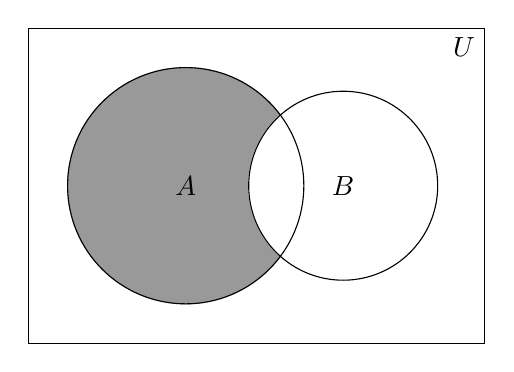
\begin{tikzpicture}
    \filldraw [gray!80] (0,0) circle (1.5);
    \filldraw [white] (2,0) circle (1.2);
    \draw (0,0) circle (1.5) node {$A$} (2,0) circle (1.2) node {$B$};
    \draw (-2,-2) rectangle (3.8,2) node [below left] {$U$};    
\end{tikzpicture} (2) 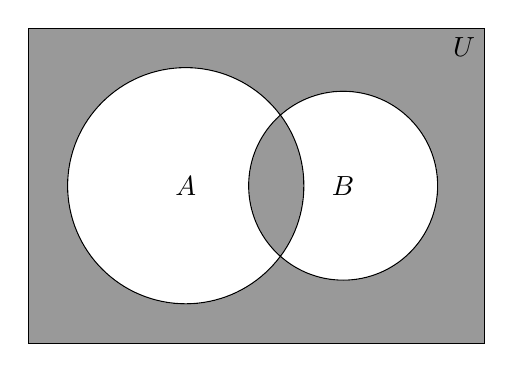
\begin{tikzpicture}
    \filldraw [gray!80] (-2,-2) rectangle (3.8,2);
    \filldraw [even odd rule, white] (0,0) circle (1.5) (2,0) circle (1.2);
    \draw (0,0) circle (1.5) node {$A$} (2,0) circle (1.2) node {$B$};
    \draw (-2,-2) rectangle (3.8,2) node [below left] {$U$};    
\end{tikzpicture}


关联目标:

暂未关联目标



标签: 第一单元

答案: 暂无答案

解答或提示: 暂无解答与提示

使用记录:

暂无使用记录


出处: 二期课改练习册高一第一学期
\item { (007703)}已知集合$A=\{1,4,x\}$, 集合$B=\{1,x^2\}$, 且$A\cup B=A$, 求$x$的值及集合$A$、$B$.


关联目标:

暂未关联目标



标签: 第一单元

答案: 暂无答案

解答或提示: 暂无解答与提示

使用记录:

暂无使用记录


出处: 二期课改练习册高一第一学期
\item { (007704)}已知集合$A=\{x|-2\le x\le 4\}$, 集合$B=\{x|-3<x<2\}$, 集合$C=\{x|-3\le x<0\}$, 求$A\cup B$, $(A\cap B)\cup C$, $(A\cup C)\cap (B\cup C)$.


关联目标:

暂未关联目标



标签: 第一单元

答案: 暂无答案

解答或提示: 暂无解答与提示

使用记录:

暂无使用记录


出处: 二期课改练习册高一第一学期
\item { (007705)}已知集合$U=\{x|x\ge 2\}$, 集合$A=\{y|3\le y<4\}$, 集合$B=\{z|2\le z<5\}$, 求$\complement _UA\cap B$, $\complement _UB\cup A$.


关联目标:

暂未关联目标



标签: 第一单元

答案: 暂无答案

解答或提示: 暂无解答与提示

使用记录:

暂无使用记录


出处: 二期课改练习册高一第一学期
\item { (007706)}已知集合$U=\{a,b,c,d,e,f\}$, 集合$A=\{a,b,c,d\}$, $A\cap B=\{a\}$, $\complement _U(A\cup B)=\{f\}$, 求集合$B$.


关联目标:

暂未关联目标



标签: 第一单元

答案: 暂无答案

解答或提示: 暂无解答与提示

使用记录:

暂无使用记录


出处: 二期课改练习册高一第一学期
\item { (007707)}判断下列语句是否为命题, 并在相应的括号内填入``是''或``否''.\\
(1) 正方形是四边形; \blank{20}\\
(2) $0$是自然数吗; \blank{20}\\
(3) 交集和并集; \blank{20}\\
(4) $3<\pi$. \blank{20}


关联目标:

暂未关联目标



标签: 第一单元

答案: 暂无答案

解答或提示: 暂无解答与提示

使用记录:

暂无使用记录


出处: 二期课改练习册高一第一学期
\item { (007708)}判断下列命题的真假, 并在相应的括号内填入``真命题''或``假命题''.\\
(1) 如果$a$、$b$都是奇数, 那么$a+b$是偶数; \blank{20}\\
(2) 一组对边平行且两对角线相等的四边形是平行四边形; \blank{20}\\
(3) 如果$|a|<2$, 那么$a<2$; \blank{20}\\
(4) 如果$A\cap B=A$, 那么$A\cup B=B$. \blank{20}


关联目标:

暂未关联目标



标签: 第一单元

答案: 暂无答案

解答或提示: 暂无解答与提示

使用记录:

暂无使用记录


出处: 二期课改练习册高一第一学期
\item { (007710)}已知命题$A$: 如果$x<3$, 那么$x<5$; 命题$B$: 如果$x\ge 3$, 那么$x\ge 5$; 命题$C$: 如果$x\ge 5$, 那么$x\ge 3$.填写各命题之间的关系:
$A$与$B$互为\blank{20}命题, $B$与$C$互为\blank{20}命题, $C$与$A$互为\blank{20}命题.


关联目标:

暂未关联目标



标签: 第一单元

答案: 暂无答案

解答或提示: 暂无解答与提示

使用记录:

暂无使用记录


出处: 二期课改练习册高一第一学期
\item { (007711)}写出命题``在$\triangle ABC$中, 如果$\angle C>\angle B$, 那么$AB>AC$''的逆命题、否命题和逆否命题, 并判断其真假.


关联目标:

暂未关联目标



标签: 第一单元

答案: 暂无答案

解答或提示: 暂无解答与提示

使用记录:

暂无使用记录


出处: 二期课改练习册高一第一学期
\item { (007712)}写出命题``如果$\alpha$, 那么$\beta$''的逆命题、否命题和逆否命题.


关联目标:

暂未关联目标



标签: 第一单元

答案: 暂无答案

解答或提示: 暂无解答与提示

使用记录:

暂无使用记录


出处: 二期课改练习册高一第一学期
\item { (007713)}写出命题``已知$a$、$b$、$c$是实数, 如果$ac<0$, 那么$ax^2+bx+c=0(a\ne 0)$有实数根''的逆命题.否命题和逆否命题, 并判断其真假.


关联目标:

暂未关联目标



标签: 第一单元

答案: 暂无答案

解答或提示: 暂无解答与提示

使用记录:

暂无使用记录


出处: 二期课改练习册高一第一学期
\item { (007714)}命题``若$x\ne 3$且$x\ne 4$, 则$x^2-7x+12\ne 0$''的逆否命题是\bracket{20}.
\twoch{若$x^2-7x+12=0$, 则$x=3$或$x=4$}{若$x^2-7x+12=0$, 则$x\ne 3$或$x\ne 4$}{若$x^2-7x+12\ne 0$, 则$x\ne 3$且$x\ne 4$}{若$x^2-7x+12=0$, 则$x=3$且$x=4$}


关联目标:

暂未关联目标



标签: 第一单元

答案: 暂无答案

解答或提示: 暂无解答与提示

使用记录:

暂无使用记录


出处: 二期课改练习册高一第一学期
\item { (007715)}如果命题$A$的逆命题是$B$, 命题$A$的否命题是$C$, 那么命题$B$是命题$C$的\bracket{20}.
\fourch{逆命题}{否命题}{逆否命题}{以上都不正确}


关联目标:

暂未关联目标



标签: 第一单元

答案: 暂无答案

解答或提示: 暂无解答与提示

使用记录:

暂无使用记录


出处: 二期课改练习册高一第一学期
\item { (007716)}试判断命题$A$: ``在$\triangle ABC$中, $BC^2=AC^2+AB^2$''与命题$B$: ``$\triangle ABC$是直角三角形''是否为等价命题, 并说明理由.


关联目标:

暂未关联目标



标签: 第一单元

答案: 暂无答案

解答或提示: 暂无解答与提示

使用记录:

暂无使用记录


出处: 二期课改练习册高一第一学期
\item { (007717)}试判断命题$A$: ``三角形任意两边之和大于第三边''与命题$B$: ``三角形任意两边之差小于第三边''是否为等价命题, 并说明理由.


关联目标:

暂未关联目标



标签: 第一单元

答案: 暂无答案

解答或提示: 暂无解答与提示

使用记录:

暂无使用记录


出处: 二期课改练习册高一第一学期
\item { (007718)}求证: 对角线不互相平分的四边形不是平行四边形.


关联目标:

暂未关联目标



标签: 第一单元

答案: 暂无答案

解答或提示: 暂无解答与提示

使用记录:

暂无使用记录


出处: 二期课改练习册高一第一学期
\item { (007720)}若$\alpha$: $\{2\}\subsetneqq B\subseteq \{2,3,4\}$, $\beta :B=\{2,4\}$, 则$\alpha$与$\beta$的推出关系是\bracket{20}.
\fourch{$\alpha \Rightarrow \beta$}{$\beta \Rightarrow \alpha$}{$\alpha \Leftrightarrow \beta$}{$\alpha \not\Rightarrow \beta$且$\beta \not\Rightarrow \alpha$}
(2)由命题甲成立, 可推出命题乙不成立, 下列说法一定正确的是\bracket{20}.
\twoch{命题甲不成立, 可推出命题乙成立}{命题甲不成立, 可推出命题乙不成立}{命题乙成立, 可推出命题甲成立}{命题乙成立, 可推出命题甲不成立}


关联目标:

暂未关联目标



标签: 第一单元

答案: 暂无答案

解答或提示: 暂无解答与提示

使用记录:

暂无使用记录


出处: 二期课改练习册高一第一学期
\item { (007721)}已知一个命题的否命题是``两组对边分别相等的四边形是平行四边形'', 试写出原命题的逆命题, 并判断原命题的真假.


关联目标:

暂未关联目标



标签: 第一单元

答案: 暂无答案

解答或提示: 暂无解答与提示

使用记录:

暂无使用记录


出处: 二期课改练习册高一第一学期
\item { (007722)}已知一个命题的逆命题是``若实数$a$、$b$满足$a=1$且$b=2$, 则$a+b<4$'', 试写出原命题的否命题, 并判断原命题的真假.


关联目标:

暂未关联目标



标签: 第一单元

答案: 暂无答案

解答或提示: 暂无解答与提示

使用记录:

暂无使用记录


出处: 二期课改练习册高一第一学期
\item { (007723)}类比$A\subseteq B\Leftrightarrow A\cap B=A$, 试再写出两个等价命题:\\
$A\subseteq B\Leftrightarrow$\blank{50};\\
$A\subseteq B\Leftrightarrow$\blank{50}.


关联目标:

暂未关联目标



标签: 第一单元

答案: 暂无答案

解答或提示: 暂无解答与提示

使用记录:

暂无使用记录


出处: 二期课改练习册高一第一学期
\item { (007724)}下列各题中命题$P$是命题$Q$的什么条件?\\
(1) $P$: 四边形的四条边相等, $Q$: 四边形是正方形;\\
(2) $P$: $\triangle ABC\cong \triangle DEF$,	$Q$: $\triangle ABC$的面积$=\triangle DEF$的面积;\\
(3) $P$: $x$是$2$的倍数, $Q$: $x$是$6$的倍数;\\
(4) $P$: 两个三角形全等, $Q$: 两个三角形的两角和一边对应相等.


关联目标:

暂未关联目标



标签: 第一单元

答案: 暂无答案

解答或提示: 暂无解答与提示

使用记录:

暂无使用记录


出处: 二期课改练习册高一第一学期
\item { (007725)}若$x$、$y$都是实数, 则``$xy=0$''是``$x=0$''的\blank{50}条件.


关联目标:

暂未关联目标



标签: 第一单元

答案: 暂无答案

解答或提示: 暂无解答与提示

使用记录:

暂无使用记录


出处: 二期课改练习册高一第一学期
\item { (007726)}若$x$、$y$、$z$都是实数, 则``$x\cdot y=y\cdot z$''是``$x=z$''的\blank{50}条件.


关联目标:

暂未关联目标



标签: 第一单元

答案: 暂无答案

解答或提示: 暂无解答与提示

使用记录:

暂无使用记录


出处: 二期课改练习册高一第一学期
\item { (007727)}若$x$、$y$、$z$都是实数, 则``$\dfrac xy=\dfrac yz$''是``$xz=y^2$''的\blank{50}条件.


关联目标:

暂未关联目标



标签: 第一单元

答案: 暂无答案

解答或提示: 暂无解答与提示

使用记录:

暂无使用记录


出处: 二期课改练习册高一第一学期
\item { (007728)}若$x$、$y$都是实数, 则``$|x|>|y|$''是``$x>y>0$''的\blank{50}条件.


关联目标:

暂未关联目标



标签: 第一单元

答案: 暂无答案

解答或提示: 暂无解答与提示

使用记录:

暂无使用记录


出处: 二期课改练习册高一第一学期
\item { (007729)}已知$l$、$m$、$n$都是自然数, ``$l+m+n$为偶数''是``$l$、$m$、$n$都是偶数''的什么条件? 为什么?


关联目标:

暂未关联目标



标签: 第一单元

答案: 暂无答案

解答或提示: 暂无解答与提示

使用记录:

暂无使用记录


出处: 二期课改练习册高一第一学期
\item { (007730)}有下列四组命题:
\textcircled{1} $P$: 集合$A\subseteq B$, $B\subseteq C$, $C\subseteq A$, 		$Q$: 集合$A=B=C$;
\textcircled{2} $P$: $A\cap B=A\cap C$, 					$Q$: $B=C$;
\textcircled{3} $P$: $(x-2)(x-3)=0$, 				$Q$: $\dfrac{x-2}{x-3}=0$;
\textcircled{4} $P$: 抛物线$y=ax^2+bx+c(a\ne 0)$过原点, $Q$: $c=0$.
其中$P$是$Q$的充要条件的有\bracket{20}.
\fourch{\textcircled{1} 、\textcircled{2} }{\textcircled{1} 、\textcircled{4} }{\textcircled{2} 、\textcircled{3} }{\textcircled{2} 、\textcircled{4}}


关联目标:

暂未关联目标



标签: 第一单元

答案: 暂无答案

解答或提示: 暂无解答与提示

使用记录:

暂无使用记录


出处: 二期课改练习册高一第一学期
\item { (007731)}写出使实数$a$、$b$一正一负的充要条件.


关联目标:

暂未关联目标



标签: 第一单元

答案: 暂无答案

解答或提示: 暂无解答与提示

使用记录:

暂无使用记录


出处: 二期课改练习册高一第一学期
\item { (007732)}求证: 实数$a$、$b$均大于$0$的充要条件是$\begin{cases} a+b>0, \\ ab>0. \end{cases}$


关联目标:

暂未关联目标



标签: 第一单元

答案: 暂无答案

解答或提示: 暂无解答与提示

使用记录:

暂无使用记录


出处: 二期课改练习册高一第一学期
\item { (007733)}命题``$x\in M$或$x\in P$''是命题``$x\in M\cap P$''的什么条件?


关联目标:

暂未关联目标



标签: 第一单元

答案: 暂无答案

解答或提示: 暂无解答与提示

使用记录:

暂无使用记录


出处: 二期课改练习册高一第一学期
\item { (007734)}写出命题``$x>3$''的一个充分条件和一个必要条件.


关联目标:

暂未关联目标



标签: 第一单元

答案: 暂无答案

解答或提示: 暂无解答与提示

使用记录:

暂无使用记录


出处: 二期课改练习册高一第一学期
\item { (007735)}如果$\alpha$是$\beta$的充分非必要条件, 那么$\overline{\alpha }$是$\overline{\beta }$的什么条件?


关联目标:

暂未关联目标



标签: 第一单元

答案: 暂无答案

解答或提示: 暂无解答与提示

使用记录:

暂无使用记录


出处: 二期课改练习册高一第一学期
\item { (007737)}填空:
已知集合$A=\{a|a$具有性质$p\}$, $B=\{b|b$具有性质$q\}$.\\
(1) 若$A\subseteq B$, 则$p$是$q$的\blank{50}条件;\\
(2) 若$A\supseteq B$, 则$p$是$q$的\blank{50}条件;\\
(3) 若$A=B$, 则$p$是$q$的\blank{50}条件.


关联目标:

暂未关联目标



标签: 第一单元

答案: 暂无答案

解答或提示: 暂无解答与提示

使用记录:

暂无使用记录


出处: 二期课改练习册高一第一学期
\item { (007738)}试用子集与推出关系来判断命题$A$是命题$B$的什么条件.\\
(1) $A$: 该平面图形是四边形, $B$: 该平面图形是梯形;\\
(2) $A$: $x=2$, $B$: $(x-5)(x-2)=0$;\\
(3) $A$: $x^2=y^2$, $B$: $x=y$;\\
(4) $A$: $a=2$, $B$: $a\le 2$.


关联目标:

暂未关联目标



标签: 第一单元

答案: 暂无答案

解答或提示: 暂无解答与提示

使用记录:

暂无使用记录


出处: 二期课改练习册高一第一学期
\item { (007739)}如果命题$p$: $m<-3$, 命题$q$: 方程$x^2-x-m=0$无实数根, 那么$p$是$q$的什么条件?


关联目标:

暂未关联目标



标签: 第一单元

答案: 暂无答案

解答或提示: 暂无解答与提示

使用记录:

暂无使用记录


出处: 二期课改练习册高一第一学期
\item { (007740)}已知命题$\alpha$: $2\le x<4$, 命题$\beta$: $3m-1\le x\le -m$, 且$\alpha$是$\beta$的充分条件, 求实数$m$的取值范围.


关联目标:

暂未关联目标



标签: 第一单元

答案: 暂无答案

解答或提示: 暂无解答与提示

使用记录:

暂无使用记录


出处: 二期课改练习册高一第一学期
\item { (007741)}如果命题$p$: $A\subseteq B$, 命题$q$: $A\subsetneqq B$, 那么$p$是$q$的什么条件?


关联目标:

暂未关联目标



标签: 第一单元

答案: 暂无答案

解答或提示: 暂无解答与提示

使用记录:

暂无使用记录


出处: 二期课改练习册高一第一学期
\item { (007742)}已知$a$为实数, 写出关于$x$的方程$ax^2+2x+1=0$至少有一个实数根的一个充要条件、一个充分条件、一个必要条件.


关联目标:

暂未关联目标



标签: 第一单元

答案: 暂无答案

解答或提示: 暂无解答与提示

使用记录:

暂无使用记录


出处: 二期课改练习册高一第一学期
\item { (007743)}下列命题中正确的是\bracket{20}.
\twoch{自然数集$\mathbf{N}$中最小的数是$1$}{空集是任何集合的真子集}{如果$A\subseteq B$, 且$A\ne B$, 那么$A$是$B$的真子集}{$\{y|y=x+3,\ x\in \mathbf{N}\}$中的最小值是$4$}


关联目标:

暂未关联目标



标签: 第一单元

答案: 暂无答案

解答或提示: 暂无解答与提示

使用记录:

暂无使用记录


出处: 二期课改练习册高一第一学期
\item { (007744)}若$A\cap B=A$, 则\bracket{20}.
\fourch{$\complement _BA\cup A=\varnothing$}{$\complement _BA\cap A=\varnothing$}{$\complement _BA\cup \complement _BB=\varnothing$}{$\complement _BA\cap A=\varnothing$}


关联目标:

暂未关联目标



标签: 第一单元

答案: 暂无答案

解答或提示: 暂无解答与提示

使用记录:

暂无使用记录


出处: 二期课改练习册高一第一学期
\item { (007745)}已知$I$是全集.若$M$、$P$、$S$是$I$的$3$个子集, 则图中阴影部分所表示的集合是\bracket{20}.
\begin{center}
    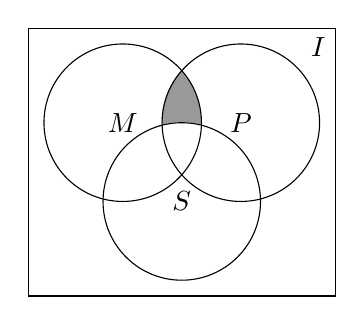
\begin{tikzpicture}
        \begin{scope}
            \clip (0,0) circle (1);
            \filldraw [gray!80] (1.5,0) circle (1);
        \end{scope}
        \filldraw [white] (0.75,-1) circle (1);
        \draw (0,0) circle (1) node {$M$};
        \draw (1.5,0) circle (1) node {$P$};
        \draw (0.75,-1) circle (1) node {$S$};
        \draw (-1.2,-2.2) rectangle (2.7,1.2) node [below left] {$I$};
    \end{tikzpicture}
\end{center}
\fourch{$(M\cap P)\cap S$}{$(M\cap P)\cup S$}{$(M\cap P)\cap \complement _IS$}{$(M\cap P)\cup \complement _IS$}


关联目标:

暂未关联目标



标签: 第一单元

答案: 暂无答案

解答或提示: 暂无解答与提示

使用记录:

暂无使用记录


出处: 二期课改练习册高一第一学期
\item { (007746)}若命题$p$: $x^2-5x+6=0$, 命题$q$: $x=2$, 则$p$是$q$的\blank{50}条件。


关联目标:

暂未关联目标



标签: 第一单元

答案: 暂无答案

解答或提示: 暂无解答与提示

使用记录:

暂无使用记录


出处: 二期课改练习册高一第一学期
\item { (007747)}若$p$: 四边形是正方形, $q$: 四边形的两条对角线互相垂直平分, 则$p$是$q$的\blank{50}条件.


关联目标:

暂未关联目标



标签: 第一单元

答案: 暂无答案

解答或提示: 暂无解答与提示

使用记录:

暂无使用记录


出处: 二期课改练习册高一第一学期
\item { (007748)}若$p$: 抛物线$y=ax^2+bx+c$过原点, $q$: $c=0$, 则$p$是$q$的\blank{50}条件.


关联目标:

暂未关联目标



标签: 第一单元

答案: 暂无答案

解答或提示: 暂无解答与提示

使用记录:

暂无使用记录


出处: 二期课改练习册高一第一学期
\item { (007749)}若$p$: $a>b$, $q$: $a^2>b^2$, 则$p$是$q$的\blank{50}条件.


关联目标:

暂未关联目标



标签: 第一单元

答案: 暂无答案

解答或提示: 暂无解答与提示

使用记录:

暂无使用记录


出处: 二期课改练习册高一第一学期
\item { (007750)}若方程$x^2+px+4=0$的解集为$A$, 方程$x^2+x+q=0$的解集为$B$, 且$A\cap B=\{4\}$, 则集合$A\cup B$的所有子集是\blank{50}.


关联目标:

暂未关联目标



标签: 第一单元

答案: 暂无答案

解答或提示: 暂无解答与提示

使用记录:

暂无使用记录


出处: 二期课改练习册高一第一学期
\item { (007751)}对上海市某校学生进行调查, 结果如下: 成语同典拥有率为$84\%$, 古汉语词典拥有率为$78\%$.同时拥有上述两种词典的学生占全校学生的$66\%$, 求上述两种词典都没有的学生所占的比例.


关联目标:

暂未关联目标



标签: 第一单元

答案: 暂无答案

解答或提示: 暂无解答与提示

使用记录:

暂无使用记录


出处: 二期课改练习册高一第一学期
\item { (007752)}已知集合$A=\{x|-2<x\le 1\}$, 集合$B=\{x|x\ge 1x<-2\}$, 求$A\cup B$, $A\cap B$.


关联目标:

暂未关联目标



标签: 第一单元

答案: 暂无答案

解答或提示: 暂无解答与提示

使用记录:

暂无使用记录


出处: 二期课改练习册高一第一学期
\item { (007753)}已知集合$A=\{x|-1<x<1$或$x\ge 3\}$, 集合$U=\{x|x\ge 2x<1\}$, 求$\complement _UA$.


关联目标:

暂未关联目标



标签: 第一单元

答案: 暂无答案

解答或提示: 暂无解答与提示

使用记录:

暂无使用记录


出处: 二期课改练习册高一第一学期
\item { (007754)}写出命题: 若$x>1$, 则$x>0$的逆命题、否命题、逆否命题, 并指出哪些是真命题.


关联目标:

暂未关联目标



标签: 第一单元

答案: 暂无答案

解答或提示: 暂无解答与提示

使用记录:

暂无使用记录


出处: 二期课改练习册高一第一学期
\item { (007755)}已知集合$A=\{x|x^2+px+q=0\}$, 集合$B=\{x|x^2-x+r=0\}$, 且$A\cap B=\{-1\}$, $A\cup B=\{-1,2\}$, 求$p$、$q$、$r$的值.


关联目标:

暂未关联目标



标签: 第一单元

答案: 暂无答案

解答或提示: 暂无解答与提示

使用记录:

暂无使用记录


出处: 二期课改练习册高一第一学期
\item { (007756)}已知全集$U=\mathbf{R}$, 集合$A=\{x|x\le a-1\}$, 集合$B=\{x|x>a+2\}$, 集合$C=\{x|x<0$或$x\ge 4\}$.若$\complement _U(A\cup B)\subseteq C$, 求实数$a$的取值范围.


关联目标:

暂未关联目标



标签: 第一单元

答案: 暂无答案

解答或提示: 暂无解答与提示

使用记录:

暂无使用记录


出处: 二期课改练习册高一第一学期
\item { (007757)}若集合$M=\{a|a=x+\sqrt 2y,\ x,y\in \mathbf{Q}\}$, 则下列结论正确的是\bracket{20}.
\fourch{$M\subseteq \mathbf{Q}$}{$M=\mathbf{Q}$}{$M\supsetneqq \mathbf{Q}$}{$M\subsetneqq \mathbf{Q}$}


关联目标:

暂未关联目标



标签: 第一单元

答案: 暂无答案

解答或提示: 暂无解答与提示

使用记录:

暂无使用记录


出处: 二期课改练习册高一第一学期
\item { (007758)}若$A$是$B$的必要非充分条件, $B$是$C$的充要条件, $C$是$D$的必要非充分条件, 则$D$是$A$的\blank{50}条件, $C$是$A$的\blank{50}条件.


关联目标:

暂未关联目标



标签: 第一单元

答案: 暂无答案

解答或提示: 暂无解答与提示

使用记录:

暂无使用记录


出处: 二期课改练习册高一第一学期
\item { (007759)}已知全集$U=\{x|x$为不大于$20$的素数$\}$.若$A\cap \complement _UB=\{3,5\}$, $\complement _UA\cap B=\{7,19\}$, $\complement _U(A\cup B)=\{2,17\}$, 则$A=$\blank{50}, $B=$\blank{50}.


关联目标:

暂未关联目标



标签: 第一单元

答案: 暂无答案

解答或提示: 暂无解答与提示

使用记录:

暂无使用记录


出处: 二期课改练习册高一第一学期
\item { (007760)}已知集合$P=\{x|-2\le x\le 5\}$, 集合$Q=\{x|k+1\le x\le 2k-1\}$, 且$Q\subseteq P$, 求实数$k$的取值范围.


关联目标:

暂未关联目标



标签: 第一单元

答案: 暂无答案

解答或提示: 暂无解答与提示

使用记录:

暂无使用记录


出处: 二期课改练习册高一第一学期
\item { (007761)}已知集合$A=\{x|(a-1)x^2+3x-2=0\}$, 是否存在这样的实数$a$, 使得集合$A$有且仅有两个子集? 若存在, 求出实数$a$的值及对应的两个子集;若不存在.请说明理由.


关联目标:

暂未关联目标



标签: 第一单元

答案: 暂无答案

解答或提示: 暂无解答与提示

使用记录:

暂无使用记录


出处: 二期课改练习册高一第一学期
\item { (007762)}解不等式: $2(x+1)-3(x-2)>8$.


关联目标:

暂未关联目标



标签: 第一单元

答案: 暂无答案

解答或提示: 暂无解答与提示

使用记录:

暂无使用记录


出处: 二期课改练习册高一第一学期
\item { (007763)}解不等式组: $\begin{cases} 3x-2(5-3x)>8, \\ 2x\le 2(2x+3). \end{cases}$


关联目标:

暂未关联目标



标签: 第一单元

答案: 暂无答案

解答或提示: 暂无解答与提示

使用记录:

暂无使用记录


出处: 二期课改练习册高一第一学期
\item { (007764)}判断下列语句是否正确, 并在相应的横线内填入``$\checkmark$''或``$\times$''.\\
(1) 若$ax>b$, 则$x>\dfrac ba(a\ne 0)$.\blank{20};\\
(2) 若$a^2x>a^2y$, 则$x>y$.\blank{20};\\
(3) 若$a>b>0$, $c>d>0$, 则$\dfrac ac>\dfrac bd$.\blank{20};\\
(4) 若$a>b$, 则$a^2>ab$.\blank{20}.


关联目标:

暂未关联目标



标签: 第一单元

答案: 暂无答案

解答或提示: 暂无解答与提示

使用记录:

暂无使用记录


出处: 二期课改练习册高一第一学期
\item { (007765)}如果$a^2>b^2$, 那么下列不等式中正确的是\bracket{20}.
\fourch{$a>0>b$}{$a>b>0$}{$|a|>|b|$}{$a>|b|$}


关联目标:

暂未关联目标



标签: 第一单元

答案: 暂无答案

解答或提示: 暂无解答与提示

使用记录:

暂无使用记录


出处: 二期课改练习册高一第一学期
\item { (007766)}如果$a<b<0$, 那么下列不等式中正确的是\bracket{20}.
\fourch{$\dfrac{-a}{-b}<1$}{$a^2>ab$}{$\dfrac 1{b^2}<\dfrac 1{a^2}$}{$\dfrac 1a<\dfrac 1b$}


关联目标:

暂未关联目标



标签: 第一单元

答案: 暂无答案

解答或提示: 暂无解答与提示

使用记录:

暂无使用记录


出处: 二期课改练习册高一第一学期
\item { (007767)}如果$a<0<b$, 那么下列不等式中正确的是\bracket{20}.
\fourch{$\sqrt {-a}<\sqrt b$}{$a^2<b^2$}{$a^3<b^3$}{$ab>b^2$}


关联目标:

暂未关联目标



标签: 第一单元

答案: 暂无答案

解答或提示: 暂无解答与提示

使用记录:

暂无使用记录


出处: 二期课改练习册高一第一学期
\item { (007768)}证明: 如果$a>b$, $c<0$, 那么$(a-b)c<0$.


关联目标:

暂未关联目标



标签: 第一单元

答案: 暂无答案

解答或提示: 暂无解答与提示

使用记录:

暂无使用记录


出处: 二期课改练习册高一第一学期
\item { (007769)}证明: 如果$a<b<0$, 那么$0>\dfrac 1a>\dfrac 1b$.


关联目标:

暂未关联目标



标签: 第一单元

答案: 暂无答案

解答或提示: 暂无解答与提示

使用记录:

暂无使用记录


出处: 二期课改练习册高一第一学期
\item { (007770)}用``$>$''或``$<$''号填空: 如果$a<b<0$, 那么\\
(1) $\sqrt [n]{-a}$\blank{50}$\sqrt [n]{-b}(n\ge 2,n\in \mathbf{N}^*)$;\\
(2) $\dfrac 1{a^{2n}}$\blank{50}$\dfrac 1{b^{2n}}(n\in \mathbf{N}^*)$.


关联目标:

暂未关联目标



标签: 第一单元

答案: 暂无答案

解答或提示: 暂无解答与提示

使用记录:

暂无使用记录


出处: 二期课改练习册高一第一学期
\item { (007771)}比较$x(x-y)$与$y(x-y)(x\ne y)$的大小.


关联目标:

暂未关联目标



标签: 第一单元

答案: 暂无答案

解答或提示: 暂无解答与提示

使用记录:

暂无使用记录


出处: 二期课改练习册高一第一学期
\item { (007772)}比较$(3a+1)(a+1)$与$2(a+1)^2-3$的大小.


关联目标:

暂未关联目标



标签: 第一单元

答案: 暂无答案

解答或提示: 暂无解答与提示

使用记录:

暂无使用记录


出处: 二期课改练习册高一第一学期
\item { (007773)}比较$(t+1)(t-5)$与$(t-2)^2$的大小.


关联目标:

暂未关联目标



标签: 第一单元

答案: 暂无答案

解答或提示: 暂无解答与提示

使用记录:

暂无使用记录


出处: 二期课改练习册高一第一学期
\item { (007774)}已知$a>2$, 解关于$x$的方程$ax+4<2x+a^2$.


关联目标:

暂未关联目标



标签: 第一单元

答案: 暂无答案

解答或提示: 暂无解答与提示

使用记录:

暂无使用记录


出处: 二期课改练习册高一第一学期
\item { (007775)}已知$m<1$, 解关于$x$的方程$mx+1<x+m^3$.


关联目标:

暂未关联目标



标签: 第一单元

答案: 暂无答案

解答或提示: 暂无解答与提示

使用记录:

暂无使用记录


出处: 二期课改练习册高一第一学期
\item { (007776)}已知$p\ne q$, 解关于$x$的方程$(p-q)x<p^2-q^2$.


关联目标:

暂未关联目标



标签: 第一单元

答案: 暂无答案

解答或提示: 暂无解答与提示

使用记录:

暂无使用记录


出处: 二期课改练习册高一第一学期
\item { (007777)}解关于$x$的方程$mx+4<m^2+2x$.


关联目标:

暂未关联目标



标签: 第一单元

答案: 暂无答案

解答或提示: 暂无解答与提示

使用记录:

暂无使用记录


出处: 二期课改练习册高一第一学期
\item { (007778)}甲乙两个工厂今年的产值分别为$25000$万元、$20000$万元.如果甲工厂每年增加产值$500$万元, 乙工厂每年增加产值$1000$万元, 那么几年后乙工厂的产值超过甲工厂的产值?


关联目标:

暂未关联目标



标签: 第一单元

答案: 暂无答案

解答或提示: 暂无解答与提示

使用记录:

暂无使用记录


出处: 二期课改练习册高一第一学期
\item { (007779)}如果$a>b$, 那么$\dfrac 1a<\dfrac 1b$成立的充要条件是\blank{50}.


关联目标:

暂未关联目标



标签: 第一单元

答案: 暂无答案

解答或提示: 暂无解答与提示

使用记录:

暂无使用记录


出处: 二期课改练习册高一第一学期
\item { (007780)}解关于$x$的不等式: $a^2(x-1)>b^2(1+x)+2ab$, 其中$a$、$b\in \mathbf{R}^+$.


关联目标:

暂未关联目标



标签: 第一单元

答案: 暂无答案

解答或提示: 暂无解答与提示

使用记录:

暂无使用记录


出处: 二期课改练习册高一第一学期
\item { (007781)}已知$x$、$y\in \mathbf{R}$, 比较$x^2+y^2$与$2(2x-y)-5$的大小.


关联目标:

暂未关联目标



标签: 第一单元

答案: 暂无答案

解答或提示: 暂无解答与提示

使用记录:

暂无使用记录


出处: 二期课改练习册高一第一学期
\item { (007782)}解不等式: $2x^2-3x+1<0$.


关联目标:

暂未关联目标



标签: 第一单元

答案: 暂无答案

解答或提示: 暂无解答与提示

使用记录:

暂无使用记录


出处: 二期课改练习册高一第一学期
\item { (007783)}解不等式: $(x+1)^2-6>0$.


关联目标:

暂未关联目标



标签: 第一单元

答案: 暂无答案

解答或提示: 暂无解答与提示

使用记录:

暂无使用记录


出处: 二期课改练习册高一第一学期
\item { (007784)}解不等式: $x(x-1)<x(2x-3)+1$.


关联目标:

暂未关联目标



标签: 第一单元

答案: 暂无答案

解答或提示: 暂无解答与提示

使用记录:

暂无使用记录


出处: 二期课改练习册高一第一学期
\item { (007785)}解不等式: $-x^2+2x+35>0$.


关联目标:

暂未关联目标



标签: 第一单元

答案: 暂无答案

解答或提示: 暂无解答与提示

使用记录:

暂无使用记录


出处: 二期课改练习册高一第一学期
\item { (007786)}解不等式: $(x-2)(3-x)\le 0$.


关联目标:

暂未关联目标



标签: 第一单元

答案: 暂无答案

解答或提示: 暂无解答与提示

使用记录:

暂无使用记录


出处: 二期课改练习册高一第一学期
\item { (007787)}解不等式: $2x-1\ge x^2$.


关联目标:

暂未关联目标



标签: 第一单元

答案: 暂无答案

解答或提示: 暂无解答与提示

使用记录:

暂无使用记录


出处: 二期课改练习册高一第一学期
\item { (007788)}解关于$x$的不等式: $(x-a)(x-1)<0(a>1)$.


关联目标:

暂未关联目标



标签: 第一单元

答案: 暂无答案

解答或提示: 暂无解答与提示

使用记录:

暂无使用记录


出处: 二期课改练习册高一第一学期
\item { (007789)}解关于$x$的不等式: $(x-a)(x-2a)<0(a>0)$.


关联目标:

暂未关联目标



标签: 第一单元

答案: 暂无答案

解答或提示: 暂无解答与提示

使用记录:

暂无使用记录


出处: 二期课改练习册高一第一学期
\item { (007790)}写出一个解集只含一个元素的一元二次不等式.


关联目标:

暂未关联目标



标签: 第一单元

答案: 暂无答案

解答或提示: 暂无解答与提示

使用记录:

暂无使用记录


出处: 二期课改练习册高一第一学期
\item { (007791)}解不等式组: $\begin{cases} 6-x-x^2\le 0, \\ x^2+3x-4<0. \end{cases}$.


关联目标:

暂未关联目标



标签: 第一单元

答案: 暂无答案

解答或提示: 暂无解答与提示

使用记录:

暂无使用记录


出处: 二期课改练习册高一第一学期
\item { (007792)}解不等式组: $\begin{cases} 4x^2-27x+18>0, \\ x^2-6x+4<0. \end{cases}$.


关联目标:

暂未关联目标



标签: 第一单元

答案: 暂无答案

解答或提示: 暂无解答与提示

使用记录:

暂无使用记录


出处: 二期课改练习册高一第一学期
\item { (007793)}已知集合$U=\mathbf{R}$, 且集合$A=\{x|x^2-16<0\}$, 集合$B=\{x|x^2-4x+3\ge 0\}$, 求:\\
(1) $A\cap B$;\\
(2) $A\cup B$;\\
(3) $\complement _U(A\cap B)$;\\
(4) $\complement _UA\cup \complement _UB$.


关联目标:

暂未关联目标



标签: 第一单元

答案: 暂无答案

解答或提示: 暂无解答与提示

使用记录:

暂无使用记录


出处: 二期课改练习册高一第一学期
\item { (007794)}已知不等式$x^2+ax+b<0$的解集为$(-3,-1)$, 求实数$a$、$b$的值.


关联目标:

暂未关联目标



标签: 第一单元

答案: 暂无答案

解答或提示: 暂无解答与提示

使用记录:

暂无使用记录


出处: 二期课改练习册高一第一学期
\item { (007795)}已知关于$x$的二次方程$2x^2+ax+1=0$无实数解, 求实数$a$的取值范围.


关联目标:

暂未关联目标



标签: 第一单元

答案: 暂无答案

解答或提示: 暂无解答与提示

使用记录:

暂无使用记录


出处: 二期课改练习册高一第一学期
\item { (007796)}已知$P(a,b)$为正比例函数$y=2x$的图像上的点, 且$P$与$B(2,-1)$之间的距离不超过$3$, 求$a$的取值范围.


关联目标:

暂未关联目标



标签: 第一单元

答案: 暂无答案

解答或提示: 暂无解答与提示

使用记录:

暂无使用记录


出处: 二期课改练习册高一第一学期
\item { (007797)}某船从甲码头沿河顺流航行$75$千米到达乙码头, 停留$30$分钟后再逆流航行$126$千米到达丙码头.如果水流的速度为每小时$4$千米, 该船要在$5$小时内完成航行任务, 那么船的速度每小时至少为多少千米?


关联目标:

暂未关联目标



标签: 第一单元

答案: 暂无答案

解答或提示: 暂无解答与提示

使用记录:

暂无使用记录


出处: 二期课改练习册高一第一学期
\item { (007798)}解不等式组: $\begin{cases} 3x^2+x-2\ge 0, \\ 4x^2-15x+9>0. \end{cases}$


关联目标:

暂未关联目标



标签: 第一单元

答案: 暂无答案

解答或提示: 暂无解答与提示

使用记录:

暂无使用记录


出处: 二期课改练习册高一第一学期
\item { (007799)}已知关于$x$的不等式组$\begin{cases} (2x-3)(3x+2)\le 0, \\ x-a>0 \end{cases}$无实数解, 求实数$a$的取值范围.


关联目标:

暂未关联目标



标签: 第一单元

答案: 暂无答案

解答或提示: 暂无解答与提示

使用记录:

暂无使用记录


出处: 二期课改练习册高一第一学期
\item { (007800)}当$k$取何值时, 关于$x$的不等式$2kx^2+kx-\dfrac 38<0$对于一切实数$x$都成立?


关联目标:

暂未关联目标



标签: 第一单元

答案: 暂无答案

解答或提示: 暂无解答与提示

使用记录:

暂无使用记录


出处: 二期课改练习册高一第一学期
\item { (007801)}已知关于$x$的不等式$ax^2+bx+c>0$的解集是$\{x|x>2$或$x<\dfrac 12\}$, 求关于$x$的不等式$ax^2-bx+c\le 0$的解集.


关联目标:

暂未关联目标



标签: 第一单元

答案: 暂无答案

解答或提示: 暂无解答与提示

使用记录:

暂无使用记录


出处: 二期课改练习册高一第一学期
\item { (007802)}某商品每件成本为$80$元, 售价为$100$元, 每天售出$100$件.若售价降低$x$成($1$成即$10\%$), 售出商品的数量就增加$\dfrac 85x$成.若要求该商品一天的营业额至少为$10260$元, 且又不能亏本, 求$x$的取值范围.


关联目标:

暂未关联目标



标签: 第一单元

答案: 暂无答案

解答或提示: 暂无解答与提示

使用记录:

暂无使用记录


出处: 二期课改练习册高一第一学期
\item { (007803)}解不等式: $\dfrac 1x<1$.


关联目标:

暂未关联目标



标签: 第一单元

答案: 暂无答案

解答或提示: 暂无解答与提示

使用记录:

暂无使用记录


出处: 二期课改练习册高一第一学期
\item { (007804)}解不等式: $\dfrac{4x+3}{x-1}>5$.


关联目标:

暂未关联目标



标签: 第一单元

答案: 暂无答案

解答或提示: 暂无解答与提示

使用记录:

暂无使用记录


出处: 二期课改练习册高一第一学期
\item { (007805)}解不等式: $\dfrac 2x<\dfrac 2{x-3}$.


关联目标:

暂未关联目标



标签: 第一单元

答案: 暂无答案

解答或提示: 暂无解答与提示

使用记录:

暂无使用记录


出处: 二期课改练习册高一第一学期
\item { (007806)}解不等式: $\dfrac 1{x-4}\le 1-\dfrac x{4-x}$.


关联目标:

暂未关联目标



标签: 第一单元

答案: 暂无答案

解答或提示: 暂无解答与提示

使用记录:

暂无使用记录


出处: 二期课改练习册高一第一学期
\item { (007807)}求当$k$为何值时, 关于$x$的方程$\dfrac{4k-3x}{k+2}=2x$的解分别是:\\
(1) 正数;\\
(2) 负数.


关联目标:

暂未关联目标



标签: 第一单元

答案: 暂无答案

解答或提示: 暂无解答与提示

使用记录:

暂无使用记录


出处: 二期课改练习册高一第一学期
\item { (007808)}解不等式: $|x^2-3|<2$.


关联目标:

暂未关联目标



标签: 第一单元

答案: 暂无答案

解答或提示: 暂无解答与提示

使用记录:

暂无使用记录


出处: 二期课改练习册高一第一学期
\item { (007809)}解不等式: $|\dfrac 1{2-x}|\ge 2$.


关联目标:

暂未关联目标



标签: 第一单元

答案: 暂无答案

解答或提示: 暂无解答与提示

使用记录:

暂无使用记录


出处: 二期课改练习册高一第一学期
\item { (007810)}解不等式: $|x^2-3x+2|\le 0$.


关联目标:

暂未关联目标



标签: 第一单元

答案: 暂无答案

解答或提示: 暂无解答与提示

使用记录:

暂无使用记录


出处: 二期课改练习册高一第一学期
\item { (007811)}解不等式: $|\dfrac x{x+1}|>\dfrac x{x+1}$.


关联目标:

暂未关联目标



标签: 第一单元

答案: 暂无答案

解答或提示: 暂无解答与提示

使用记录:

暂无使用记录


出处: 二期课改练习册高一第一学期
\item { (007812)}解不等式: $|x-3|<x-1$.


关联目标:

暂未关联目标



标签: 第一单元

答案: 暂无答案

解答或提示: 暂无解答与提示

使用记录:

暂无使用记录


出处: 二期课改练习册高一第一学期
\item { (007813)}若$a<b<0$, 则不等式$\dfrac{x+a}{x+b}>0$的解集是\blank{50}.


关联目标:

暂未关联目标



标签: 第一单元

答案: 暂无答案

解答或提示: 暂无解答与提示

使用记录:

暂无使用记录


出处: 二期课改练习册高一第一学期
\item { (007814)}解不等式: $4\le|x^2-4x|<5$.


关联目标:

暂未关联目标



标签: 第一单元

答案: 暂无答案

解答或提示: 暂无解答与提示

使用记录:

暂无使用记录


出处: 二期课改练习册高一第一学期
\item { (007815)}解不等式: $\dfrac 1{|x|}>x$.


关联目标:

暂未关联目标



标签: 第一单元

答案: 暂无答案

解答或提示: 暂无解答与提示

使用记录:

暂无使用记录


出处: 二期课改练习册高一第一学期
\item { (007816)}已知不等式$|ax+1|\le b$的解集是$[-1,3]$, 求$a$、$b$的值.


关联目标:

暂未关联目标



标签: 第一单元

答案: 暂无答案

解答或提示: 暂无解答与提示

使用记录:

暂无使用记录


出处: 二期课改练习册高一第一学期
\item { (007817)}如果$a$、$b\in \mathbf{R}$, 且$ab>0$, 那么下列不等式中正确的是\bracket{20}.
\fourch{$a^2+b^2>2ab$}{$a+b\ge 2\sqrt {ab}$}{$\dfrac 1a+\dfrac 1b>\dfrac 2{\sqrt {ab}}$}{$\dfrac ba+\dfrac ab\ge 2$}


关联目标:

暂未关联目标



标签: 第一单元

答案: 暂无答案

解答或提示: 暂无解答与提示

使用记录:

暂无使用记录


出处: 二期课改练习册高一第一学期
\item { (007818)}设$ab\ne 0$, 利用基本不等式有如下证明: $\dfrac ba+\dfrac ab=\dfrac{{b^2}+{a^2}}{ab}\ge \dfrac{2ab}{ab}=2$. 试判断这个证明过程是否正确. 若正确, 请说明每一步的依据; 若不正确, 请说明理由.


关联目标:

暂未关联目标



标签: 第一单元

答案: 暂无答案

解答或提示: 暂无解答与提示

使用记录:

暂无使用记录


出处: 二期课改练习册高一第一学期
\item { (007819)}已知$a$、$b\in \mathbf{R}$, 比较$|a|+\dfrac{|b|}2$与$\sqrt 2\cdot \sqrt {|ab|}$的大小.


关联目标:

暂未关联目标



标签: 第一单元

答案: 暂无答案

解答或提示: 暂无解答与提示

使用记录:

暂无使用记录


出处: 二期课改练习册高一第一学期
\item { (007820)}已知$0<x<\dfrac 12$, 求当$x$取何值时, $x(1-2x)$的值最大.


关联目标:

暂未关联目标



标签: 第一单元

答案: 暂无答案

解答或提示: 暂无解答与提示

使用记录:

暂无使用记录


出处: 二期课改练习册高一第一学期
\item { (007821)}已知$a>0$, 求证: $a+a^3\ge 2a^2$.


关联目标:

暂未关联目标



标签: 第一单元

答案: 暂无答案

解答或提示: 暂无解答与提示

使用记录:

暂无使用记录


出处: 二期课改练习册高一第一学期
\item { (007822)}用一根长为$l$的铁丝制成一个矩形框架.当长、宽分别为多少时, 框架的面积最大?


关联目标:

暂未关联目标



标签: 第一单元

答案: 暂无答案

解答或提示: 暂无解答与提示

使用记录:

暂无使用记录


出处: 二期课改练习册高一第一学期
\item { (007823)}已知$x$、$y\in \mathbf{R}^+$, 且$x+y=1$, 求当$x$、$y$分别取何值时, $\dfrac 1x+\dfrac 1y$的值最小.


关联目标:

暂未关联目标



标签: 第一单元

答案: 暂无答案

解答或提示: 暂无解答与提示

使用记录:

暂无使用记录


出处: 二期课改练习册高一第一学期
\item { (007824)}已知$x>-1$, 求当$x$取何值时, $x+\dfrac 4{x+1}$的值最小.


关联目标:

暂未关联目标



标签: 第一单元

答案: 暂无答案

解答或提示: 暂无解答与提示

使用记录:

暂无使用记录


出处: 二期课改练习册高一第一学期
\item { (007825)}已知$a+b=1$, 求证: $a^2+b^2\ge \dfrac 12$.


关联目标:

暂未关联目标



标签: 第一单元

答案: 暂无答案

解答或提示: 暂无解答与提示

使用记录:

暂无使用记录


出处: 二期课改练习册高一第一学期
\item { (007826)}建造一个容积为$8$立方米、深为$2$米的长方形无盖水池.如果池底和池壁的造价每平方米分别为$120$元和$80$元, 那么水池的最低造价是多少元?


关联目标:

暂未关联目标



标签: 第一单元

答案: 暂无答案

解答或提示: 暂无解答与提示

使用记录:

暂无使用记录


出处: 二期课改练习册高一第一学期
\item { (007827)}求证: $(ac+bd)^2\le (a^2+b^2)(c^2+d^2)$.


关联目标:

暂未关联目标



标签: 第一单元

答案: 暂无答案

解答或提示: 暂无解答与提示

使用记录:

暂无使用记录


出处: 二期课改练习册高一第一学期
\item { (007828)}已知$x>y$, 求证: $x^3-y^3>x^2y-xy^2$.


关联目标:

暂未关联目标



标签: 第一单元

答案: 暂无答案

解答或提示: 暂无解答与提示

使用记录:

暂无使用记录


出处: 二期课改练习册高一第一学期
\item { (007829)}已知实数$a\ge 3$, 求证: $\sqrt a-\sqrt {a-1}<\sqrt {a-2}-\sqrt {a-3}$.


关联目标:

暂未关联目标



标签: 第一单元

答案: 暂无答案

解答或提示: 暂无解答与提示

使用记录:

暂无使用记录


出处: 二期课改练习册高一第一学期
\item { (007830)}已知$a$、$b$、$c$是不全相等的整数, 求证: $(a^2+1)(b^2+1)(c^2+1)>8abc$.


关联目标:

暂未关联目标



标签: 第一单元

答案: 暂无答案

解答或提示: 暂无解答与提示

使用记录:

暂无使用记录


出处: 二期课改练习册高一第一学期
\item { (007831)}设$a$、$b$、$c\in \mathbf{R}^+$, 求证: $\dfrac{b+c}a+\dfrac{c+a}b+\dfrac{a+b}c\ge 6$.


关联目标:

暂未关联目标



标签: 第一单元

答案: 暂无答案

解答或提示: 暂无解答与提示

使用记录:

暂无使用记录


出处: 二期课改练习册高一第一学期
\item { (007832)}已知$a>0$, $b>0$, 求证: $\dfrac a{\sqrt b}+\dfrac b{\sqrt a}\ge \sqrt a+\sqrt b$.


关联目标:

暂未关联目标



标签: 第一单元

答案: 暂无答案

解答或提示: 暂无解答与提示

使用记录:

暂无使用记录


出处: 二期课改练习册高一第一学期
\item { (007833)}求证: $|\dfrac{a^2-1}{a^2+1}|\le 1$.


关联目标:

暂未关联目标



标签: 第一单元

答案: 暂无答案

解答或提示: 暂无解答与提示

使用记录:

暂无使用记录


出处: 二期课改练习册高一第一学期
\item { (007834)}如果$a\in \mathbf{R}$, 且$a^2+a<0$, 那么$a$、$a^2$、$-a$、$-a^2$的大小关系是\bracket{20}.
\fourch{$-a<-a^2<a<a^2$}{$a<-a^2<a^2<-a$}{$-a^2<a<a^2<-a$}{$-a^2<a<-a<a^2$}


关联目标:

暂未关联目标



标签: 第一单元

答案: 暂无答案

解答或提示: 暂无解答与提示

使用记录:

暂无使用记录


出处: 二期课改练习册高一第一学期
\item { (007835)}不等式$\dfrac{x^2}{x-1}\ge 0$的解是\bracket{20}.
\fourch{$(1,+\infty)$}{$[1+\infty)$}{$(1,+\infty)\cup \{0\}$}{$[1,+\infty)\cup \{0\}$}


关联目标:

暂未关联目标



标签: 第一单元

答案: 暂无答案

解答或提示: 暂无解答与提示

使用记录:

暂无使用记录


出处: 二期课改练习册高一第一学期
\item { (007836)}不等式$1+|x+1|<0$的解集是\bracket{20}.
\fourch{$(-\infty ,-2)$}{$(-2,0)$}{$\mathbf{R}$}{$\varnothing$}


关联目标:

暂未关联目标



标签: 第一单元

答案: 暂无答案

解答或提示: 暂无解答与提示

使用记录:

暂无使用记录


出处: 二期课改练习册高一第一学期
\item { (007837)}证明: 如果$a>b>0$, $c>d>0$, 那么$a^2c>b^2d$.


关联目标:

暂未关联目标



标签: 第一单元

答案: 暂无答案

解答或提示: 暂无解答与提示

使用记录:

暂无使用记录


出处: 二期课改练习册高一第一学期
\item { (007838)}证明: $a^2+b^2+2\ge 2(a+b)$.


关联目标:

暂未关联目标



标签: 第一单元

答案: 暂无答案

解答或提示: 暂无解答与提示

使用记录:

暂无使用记录


出处: 二期课改练习册高一第一学期
\item { (007839)}证明: 如果$a$、$b$、$c$都是正数, 那么$(a+b)(b+c)(c+a)\ge 8abc$.


关联目标:

暂未关联目标



标签: 第一单元

答案: 暂无答案

解答或提示: 暂无解答与提示

使用记录:

暂无使用记录


出处: 二期课改练习册高一第一学期
\item { (007840)}解不等式: $2(x+1)(x+2)>(x+3)(x+4)$.


关联目标:

暂未关联目标



标签: 第一单元

答案: 暂无答案

解答或提示: 暂无解答与提示

使用记录:

暂无使用记录


出处: 二期课改练习册高一第一学期
\item { (007841)}解不等式: $-3x^25x-4<0$.


关联目标:

暂未关联目标



标签: 第一单元

答案: 暂无答案

解答或提示: 暂无解答与提示

使用记录:

暂无使用记录


出处: 二期课改练习册高一第一学期
\item { (007842)}解不等式: $4x^2-20x+25\le 0$.


关联目标:

暂未关联目标



标签: 第一单元

答案: 暂无答案

解答或提示: 暂无解答与提示

使用记录:

暂无使用记录


出处: 二期课改练习册高一第一学期
\item { (007843)}解不等式: $x^2-16x+64>0$.


关联目标:

暂未关联目标



标签: 第一单元

答案: 暂无答案

解答或提示: 暂无解答与提示

使用记录:

暂无使用记录


出处: 二期课改练习册高一第一学期
\item { (007844)}解不等式组: $\begin{cases} x^2-16<0, \\ x^2-4x+3\ge 0. \end{cases}$.


关联目标:

暂未关联目标



标签: 第一单元

答案: 暂无答案

解答或提示: 暂无解答与提示

使用记录:

暂无使用记录


出处: 二期课改练习册高一第一学期
\item { (007845)}解不等式组: $4<x^2-x-2<10$.


关联目标:

暂未关联目标



标签: 第一单元

答案: 暂无答案

解答或提示: 暂无解答与提示

使用记录:

暂无使用记录


出处: 二期课改练习册高一第一学期
\item { (007846)}解不等式: $|\dfrac{3x-9}2|\le 6$.


关联目标:

暂未关联目标



标签: 第一单元

答案: 暂无答案

解答或提示: 暂无解答与提示

使用记录:

暂无使用记录


出处: 二期课改练习册高一第一学期
\item { (007847)}解不等式: $3<|x-2|<5$.


关联目标:

暂未关联目标



标签: 第一单元

答案: 暂无答案

解答或提示: 暂无解答与提示

使用记录:

暂无使用记录


出处: 二期课改练习册高一第一学期
\item { (007848)}解不等式: $|\dfrac 1x|<\dfrac 45$.


关联目标:

暂未关联目标



标签: 第一单元

答案: 暂无答案

解答或提示: 暂无解答与提示

使用记录:

暂无使用记录


出处: 二期课改练习册高一第一学期
\item { (007849)}下列四对不等式(组)中, 哪几对具有相同的解集?\\
(1) $-\dfrac 12x^2+3x+\dfrac{27}2>0$与$x^2-6x-27>0$;\\
(2) $4<x^2-x+2<10$与$\begin{cases} x^2-x+2<10, \\ x^2-x+2>4; \end{cases}$\\
(3) $|2x+1|<5$与$2x+1<5$或$2x+1>-5$;\\
(4) $\dfrac{x-1}{x+1}<2$与$x-1<2(x+1)$.


关联目标:

暂未关联目标



标签: 第一单元

答案: 暂无答案

解答或提示: 暂无解答与提示

使用记录:

暂无使用记录


出处: 二期课改练习册高一第一学期
\item { (007850)}已知关于$x$的不等式$2x^2-2(a-1)x+(a+3)>0$的解集是$\mathbf{R}$, 求实数$a$的取值范围.


关联目标:

暂未关联目标



标签: 第一单元

答案: 暂无答案

解答或提示: 暂无解答与提示

使用记录:

暂无使用记录


出处: 二期课改练习册高一第一学期
\item { (007851)}已知函数$y=(m-1)x^2+(m-3)x+(m-1)$, $m$取什么实数时, 函数图像与$x$轴\\
(1) 没有公共点?\\
(2) 只有一个公共点?\\
(3) 有两个不同的公共点?


关联目标:

暂未关联目标



标签: 第一单元

答案: 暂无答案

解答或提示: 暂无解答与提示

使用记录:

暂无使用记录


出处: 二期课改练习册高一第一学期
\item { (007852)}当$k$是什么实数时, 关于$x$的方程$2x+k(x+3)=4$的解是正数?


关联目标:

暂未关联目标



标签: 第一单元

答案: 暂无答案

解答或提示: 暂无解答与提示

使用记录:

暂无使用记录


出处: 二期课改练习册高一第一学期
\item { (007853)}已知直角三角形的周长为$4$, 求这个直角三角形面积的最大值, 并求此时各边的长.


关联目标:

暂未关联目标



标签: 第一单元

答案: 暂无答案

解答或提示: 暂无解答与提示

使用记录:

暂无使用记录


出处: 二期课改练习册高一第一学期
\item { (007854)}求证: $(\dfrac{a+b}2)^2\le \dfrac{a^2+b^2}2$.


关联目标:

暂未关联目标



标签: 第一单元

答案: 暂无答案

解答或提示: 暂无解答与提示

使用记录:

暂无使用记录


出处: 二期课改练习册高一第一学期
\item { (007855)}求不等式$5\le x^2-2x+2<26$的正整数解.


关联目标:

暂未关联目标



标签: 第一单元

答案: 暂无答案

解答或提示: 暂无解答与提示

使用记录:

暂无使用记录


出处: 二期课改练习册高一第一学期
\item { (007856)}已知$x$、$y\in [a,b]$.\\
(1) 求$x+y$的范围;\\
(2) 若$x<y$, 求$x-y$的范围.


关联目标:

暂未关联目标



标签: 第一单元

答案: 暂无答案

解答或提示: 暂无解答与提示

使用记录:

暂无使用记录


出处: 二期课改练习册高一第一学期
\item { (007857)}当$k$为什么实数时, 方程组$\begin{cases} 3x-6y=1, \\ 5x-ky=2 \end{cases}$的解满足$x<0$且$y<0$的条件?


关联目标:

暂未关联目标



标签: 第一单元

答案: 暂无答案

解答或提示: 暂无解答与提示

使用记录:

暂无使用记录


出处: 二期课改练习册高一第一学期
\item { (007858)}当$k$为什么实数时, 方程组$\begin{cases} 4x+3y=60, \\ kx+(k+2)y=60 \end{cases}$的解满足$x>y>0$的条件?


关联目标:

暂未关联目标



标签: 第一单元

答案: 暂无答案

解答或提示: 暂无解答与提示

使用记录:

暂无使用记录


出处: 二期课改练习册高一第一学期
\item { (007859)}已知$m<n$, 试写出一个形如$ax^2+bx+c>0$的一元二次不等式, 使它的解集分别为:\\
(1) $(-\infty ,m)\cup (n,+\infty)$;\\
(2) $(m,n)$.


关联目标:

暂未关联目标



标签: 第一单元

答案: 暂无答案

解答或提示: 暂无解答与提示

使用记录:

暂无使用记录


出处: 二期课改练习册高一第一学期
\item { (007985)}若集合$A=\{x|0.1<\dfrac 1x<0.3,\ x\in \mathbf{N}\}$, 集合$B=\{x||x|\le 5,\ x\in \mathbf{Z}\}$, 则$A\cup B$中的元素个数是\bracket{20}.
\fourch{$11$}{$13$}{$15$}{$17$}


关联目标:

暂未关联目标



标签: 第一单元

答案: 暂无答案

解答或提示: 暂无解答与提示

使用记录:

暂无使用记录


出处: 二期课改练习册高一第一学期
\item { (007986)}``$x\ne 1$且$y\ne 2$''是``$x+y\ne 3$''的\bracket{20}.
\twoch{充分非必要条件}{必要非充分条件}{充要条件}{既非充分又非必要条件}


关联目标:

暂未关联目标



标签: 第一单元

答案: 暂无答案

解答或提示: 暂无解答与提示

使用记录:

暂无使用记录


出处: 二期课改练习册高一第一学期
\item { (007988)}已知集合$A=\{x|3x^2+x-2\ge 0,\  x\in \mathbf{R}\}$, 集合$B=\{x|\dfrac{4x-3}{x-3}>0,\ x\in \mathbf{R}\}$, 求$A\cap B$.


关联目标:

暂未关联目标



标签: 第一单元

答案: 暂无答案

解答或提示: 暂无解答与提示

使用记录:

暂无使用记录


出处: 二期课改练习册高一第一学期
\item { (007990)}已知集合$A=(-2,-1)\cup (0,+\infty)$, 集合$B=\{x|x^2+ax+b\le 0\}$, 且$A\cap B=(0,2]$, $A\cup B=(-2,+\infty)$, 求实数$a$、$b$的值.


关联目标:

暂未关联目标



标签: 第一单元

答案: 暂无答案

解答或提示: 暂无解答与提示

使用记录:

暂无使用记录


出处: 二期课改练习册高一第一学期
\item { (007991)}已知关于$x$的不等式$ax^2+3ax-2<0$的解集为$\mathbf{R}$, 求实数$a$的取值范围.


关联目标:

暂未关联目标



标签: 第一单元

答案: 暂无答案

解答或提示: 暂无解答与提示

使用记录:

暂无使用记录


出处: 二期课改练习册高一第一学期
\item { (007995)}已知集合$A=\{x||x-a|<2\}$, 集合$B=\{x|\dfrac{2x-1}{x-2}<1\}$, 且$A\subseteq B$, 求实数$a$的取值范围.


关联目标:

暂未关联目标



标签: 第一单元

答案: 暂无答案

解答或提示: 暂无解答与提示

使用记录:

暂无使用记录


出处: 二期课改练习册高一第一学期
\item { (007996)}已知全集$U=\mathbf{R}$, 集合$A=\{x|x^2+px+12=0\}$, 集合$B=\{x|x-5x-q=0\}$, 满足$(\complement _UA)\cap B=\{2\}$.求实数$p$与$q$的值.


关联目标:

暂未关联目标



标签: 第一单元

答案: 暂无答案

解答或提示: 暂无解答与提示

使用记录:

暂无使用记录


出处: 二期课改练习册高一第一学期
\item { (009426)}判断下列各组对象能否组成集合. 若能组成集合, 指出是有限集还是无限集; 若不能组成集合, 请说明理由.\\
(1) 上海市现有各区的名称;\\
(2) 末位是$3$的自然数;\\
(3) 比较大的苹果.


关联目标:

暂未关联目标



标签: 第一单元

答案: 暂无答案

解答或提示: 暂无解答与提示

使用记录:

暂无使用记录


出处: 新教材必修第一册课堂练习
\item { (009427)}用符号``$\in$''或``$\not\in$''填空:\\
(1) $\dfrac12$\blank{50}$\mathbf{N}$;\\
(2) $5$\blank{50}$\mathbf{Z}$;\\
(3) $-2$\blank{50}$\mathbf{Q}$;\\
(4) $\pi$\blank{50}$\mathbf{R}$.


关联目标:

暂未关联目标



标签: 第一单元

答案: 暂无答案

解答或提示: 暂无解答与提示

使用记录:

暂无使用记录


出处: 新教材必修第一册课堂练习
\item { (009428)}用列举法表示下列集合:\\
(1) 能整除$10$的所有正整数组成的集合;\\
(2) 绝对值小于$4$的所有整数组成的集合.


关联目标:

暂未关联目标



标签: 第一单元

答案: 暂无答案

解答或提示: 暂无解答与提示

使用记录:

暂无使用记录


出处: 新教材必修第一册课堂练习
\item { (009429)}用描述法表示下列集合:\\
(1) 全体偶数组成的集合;\\
(2) 平面直角坐标系中$x$轴上所有点组成的集合.


关联目标:

暂未关联目标



标签: 第一单元

答案: 暂无答案

解答或提示: 暂无解答与提示

使用记录:

暂无使用记录


出处: 新教材必修第一册课堂练习
\item { (009430)}用区间表示下列集合:\\
(1) $\{x|-1<x\le 5\}$;\\
(2) 不等式$-2x>6$的所有解组成的集合.


关联目标:

暂未关联目标



标签: 第一单元

答案: 暂无答案

解答或提示: 暂无解答与提示

使用记录:

暂无使用记录


出处: 新教材必修第一册课堂练习
\item { (009431)}判断下列说法是否正确, 并简要说明理由:\\
(1) 若$a\in A$且$A\subseteq B$, 则$a\in B$;\\
(2) 若$A\subseteq B$且$A\subseteq C$, 则$B=C$;\\
(3) 若$A\subset B$且$B\subseteq C$, 则$A\subset C$.


关联目标:

暂未关联目标



标签: 第一单元

答案: 暂无答案

解答或提示: 暂无解答与提示

使用记录:

暂无使用记录


出处: 新教材必修第一册课堂练习
\item { (009432)}用符号``$\supset$''``$=$''或``$\subset$''填空:\\
(1) $\{a\}$\blank{50}$\{a, b, c\}$;\\
(2) $\{a, b, c\}$\blank{50}$\{a, c\}$;\\
(3) $\{1, 2\}$\blank{50}$\{x|x^2-3x+2=0\}$.


关联目标:

暂未关联目标



标签: 第一单元

答案: 暂无答案

解答或提示: 暂无解答与提示

使用记录:

暂无使用记录


出处: 新教材必修第一册课堂练习
\item { (009433)}写出所有满足$\{a\}\subset M\subset \{a, b, c, d\}$的集合$M$.


关联目标:

暂未关联目标



标签: 第一单元

答案: 暂无答案

解答或提示: 暂无解答与提示

使用记录:

暂无使用记录


出处: 新教材必修第一册课堂练习
\item { (009434)}设$A$为全集$U$的任一子集, 则
(1) $\overline{\overline{A}}=$\blank{50}; (A表示A的补集A的补集)\\
(2) $A\cap \overline A=$\blank{50};\\
(3) $A\cup \overline A=$\blank{50}.


关联目标:

暂未关联目标



标签: 第一单元

答案: 暂无答案

解答或提示: 暂无解答与提示

使用记录:

暂无使用记录


出处: 新教材必修第一册课堂练习
\item { (009435)}已知全集为$\mathbf{R}$, 集合$A=\{x|-2<x\le 1\}$. 求$A$.


关联目标:

暂未关联目标



标签: 第一单元

答案: 暂无答案

解答或提示: 暂无解答与提示

使用记录:

暂无使用记录


出处: 新教材必修第一册课堂练习
\item { (009436)}已知集合$A=\{1, 2, 3, 4, 5\}$, $B=\{2, 4, 6, 8\}$, $C=\{3, 4, 5, 6\}$. 求:\\
(1) $(A\cap B)\cup C$, $(A\cup C)\cap (B\cup C)$;\\
(2) $(A\cup B)\cap C$, $(A\cap C)\cup (B\cap C)$.


关联目标:

暂未关联目标



标签: 第一单元

答案: 暂无答案

解答或提示: 暂无解答与提示

使用记录:

暂无使用记录


出处: 新教材必修第一册课堂练习
\item { (009437)}举几个生活中的命题的例子, 并判断其真假.


关联目标:

暂未关联目标



标签: 第一单元

答案: 暂无答案

解答或提示: 暂无解答与提示

使用记录:

暂无使用记录


出处: 新教材必修第一册课堂练习
\item { (009438)}判断下列命题的真假, 并说明理由:\\
(1) 所有偶数都不是素数;\\
(2) $\{1\}$是$\{0, 1, 2\}$的真子集;\\
(3) $0$是$\{0, 1, 2\}$的真子集;\\
(4) 如果集合$A$是集合$B$的子集, 那么$B$不是$A$的子集.


关联目标:

暂未关联目标



标签: 第一单元

答案: 暂无答案

解答或提示: 暂无解答与提示

使用记录:

暂无使用记录


出处: 新教材必修第一册课堂练习
\item { (009439)}用``$\Rightarrow$''表示下列陈述句$\alpha$与$\beta$之间的推出关系:\\
(1) $\alpha: \triangle ABC$是等边三角形, $\beta: \triangle ABC$是轴对称图形;\\
(2) $\alpha: x^2=4$, $\beta: x=2$.


关联目标:

暂未关联目标



标签: 第一单元

答案: 暂无答案

解答或提示: 暂无解答与提示

使用记录:

暂无使用记录


出处: 新教材必修第一册课堂练习
\item { (009440)}已知$\alpha$: 四边形$ABCD$的两组对边分别平行, $\beta$: 四边形$ABCD$为矩形, $\gamma$: 四边形$ABCD$的两组对边分别相等. 用``充分非必要''``必要非充分''``充要''或``既非充分又非必要''填空:\\
(1) $\alpha$是$\beta$的\blank{50}条件;\\
(2) $\beta$是$\gamma$的\blank{50}条件;\\
(3) $\alpha$是$\gamma$的\blank{50}条件.


关联目标:

暂未关联目标



标签: 第一单元

答案: 暂无答案

解答或提示: 暂无解答与提示

使用记录:

暂无使用记录


出处: 新教材必修第一册课堂练习
\item { (009441)}设$\alpha: 1\le x<4$, $\beta: x<m$, $\alpha$是$\beta$的充分条件. 求实数$m$的取值范围.


关联目标:

暂未关联目标



标签: 第一单元

答案: 暂无答案

解答或提示: 暂无解答与提示

使用记录:

暂无使用记录


出处: 新教材必修第一册课堂练习
\item { (009442)}设$n\in \mathbf{Z}$. 证明: 若$n^3$是奇数, 则$n$是奇数.


关联目标:

暂未关联目标



标签: 第一单元

答案: 暂无答案

解答或提示: 暂无解答与提示

使用记录:

暂无使用记录


出处: 新教材必修第一册课堂练习
\item { (009443)}证明: 对于三个实数$a$、$b$、$c$, 若$a\ne c$, 则$a\ne b$或$b\ne c$.


关联目标:

暂未关联目标



标签: 第一单元

答案: 暂无答案

解答或提示: 暂无解答与提示

使用记录:

暂无使用记录


出处: 新教材必修第一册课堂练习
\item { (009444)}设$a$、$b$、$c$、$d$是实数, 判断下列命题的真假, 并说明理由:\\
(1) 若$a^2=b^2$, 则$a=b$;\\
(2) 若$a(c^2+1)=b(c^2+1)$, 则$a=b$;\\
(3) 若$ab=0$, 则$a=0$或$b=0$;\\
(4) 若$\dfrac ac=\dfrac bd$, 且$c+d\ne 0$, 则$\dfrac{a+b}{c+d}=\dfrac ac$.


关联目标:

暂未关联目标



标签: 第一单元

答案: 暂无答案

解答或提示: 暂无解答与提示

使用记录:

暂无使用记录


出处: 新教材必修第一册课堂练习
\item { (009445)}设$a\in \mathbf{R}$, 求关于$x$的方程$ax=a^2+x-1$的解集.


关联目标:

暂未关联目标



标签: 第一单元

答案: 暂无答案

解答或提示: 暂无解答与提示

使用记录:

暂无使用记录


出处: 新教材必修第一册课堂练习
\item { (009446)}设$k\in \mathbf{R}$, 求关于$x$与$y$的二元一次方程组$\begin{cases}y=kx+1, \\ y=2kx+3 \end{cases}$的解集.


关联目标:

暂未关联目标



标签: 第一单元

答案: 暂无答案

解答或提示: 暂无解答与提示

使用记录:

暂无使用记录


出处: 新教材必修第一册课堂练习
\item { (009447)}求一元二次方程$ax^2-4x+2=0$($a\ne 0$)的解集.


关联目标:

暂未关联目标



标签: 第一单元

答案: 暂无答案

解答或提示: 暂无解答与提示

使用记录:

暂无使用记录


出处: 新教材必修第一册课堂练习
\item { (009448)}已知方程$2x^2+4x-3=0$的两个根为$x_1$、$x_2$, 求下列各式的值:\\
(1) $x_1^2x_2+x_2^2x_1$;\\
(2) $\dfrac1{x_1}+\dfrac1{x_2}$;\\
(3) $x_1^2+x_2^2$;\\
(4) $x_1^3+x_2^3$.


关联目标:

暂未关联目标



标签: 第一单元

答案: 暂无答案

解答或提示: 暂无解答与提示

使用记录:

暂无使用记录


出处: 新教材必修第一册课堂练习
\item { (009449)}设$a$、$b$、$c$、$d$为实数, 判断下列命题的真假, 并说明理由:\\
(1) 如果$a>b$, $c>d$, 那么$a+d>b+c$;\\
(2) 如果$ab>ac$, 那么$b>c$;\\
(3) 如果$a\ge b$且$a\le b$, 那么$a=b$;\\
(4) 如果$a>b$, $\dfrac 1c>\dfrac 1d$, 那么$ac>bd$;\\
(5) 如果$\dfrac ba>\dfrac dc$, 那么$bc>ad$.


关联目标:

暂未关联目标



标签: 第一单元

答案: 暂无答案

解答或提示: 暂无解答与提示

使用记录:

暂无使用记录


出处: 新教材必修第一册课堂练习
\item { (009450)}设$ab>0$, 求证: $a>b$是$\dfrac 1a<\dfrac 1b$的充要条件.


关联目标:

暂未关联目标



标签: 第一单元

答案: 暂无答案

解答或提示: 暂无解答与提示

使用记录:

暂无使用记录


出处: 新教材必修第一册课堂练习
\item { (009451)}设$a$、$b$、$c$是实数, 判断下列命题的真假, 并说明理由.\\
(1) 如果$ac^2>bc^2$, 那么$a>b$;\\
(2) 如果$ab>c$, 那么$a>\dfrac cb$;\\
(3) 如果$a>b\ge 0$, 那么$\sqrt a>\sqrt b$.


关联目标:

暂未关联目标



标签: 第一单元

答案: 暂无答案

解答或提示: 暂无解答与提示

使用记录:

暂无使用记录


出处: 新教材必修第一册课堂练习
\item { (009452)}设$x$是实数, 比较$x^2+4$与$4x$的值的大小.


关联目标:

暂未关联目标



标签: 第一单元

答案: 暂无答案

解答或提示: 暂无解答与提示

使用记录:

暂无使用记录


出处: 新教材必修第一册课堂练习
\item { (009453)}设$a\ne 1$, 解关于$x$的不等式: $ax<a^2+x-1$.


关联目标:

暂未关联目标



标签: 第一单元

答案: 暂无答案

解答或提示: 暂无解答与提示

使用记录:

暂无使用记录


出处: 新教材必修第一册课堂练习
\item { (009454)}填空题:\\
(1) $(x-2)(x+3)<0$的解集是\blank{50};\\
(2) $(2-x)(x+3)<0$的解集是\blank{50};\\
(3) $(x-2)(x+3)\ge 0$的解集是\blank{50}.


关联目标:

暂未关联目标



标签: 第一单元

答案: 暂无答案

解答或提示: 暂无解答与提示

使用记录:

暂无使用记录


出处: 新教材必修第一册课堂练习
\item { (009455)}求下列不等式的解集:\\
(1) $-8x\le 3x^2+4$;\\
(2) $-x^2<2x-4$.


关联目标:

暂未关联目标



标签: 第一单元

答案: 暂无答案

解答或提示: 暂无解答与提示

使用记录:

暂无使用记录


出处: 新教材必修第一册课堂练习
\item { (009456)}解下列不等式:\\
(1) $x+2>-x^2$;\\
(2) $-x^2+3x-4>0$;\\
(3) $9x^2-6x+1>0$;\\
(4) $4x-x^2>4$;\\
(5) $2x^2+1\ge x$;\\
(6) $x^2+\dfrac 19\ge \dfrac 23x$.


关联目标:

暂未关联目标



标签: 第一单元

答案: 暂无答案

解答或提示: 暂无解答与提示

使用记录:

暂无使用记录


出处: 新教材必修第一册课堂练习
\item { (009457)}写出一个一元二次不等式, 使它的解集分别为:\\
(1) $(3-\sqrt 2, 3+\sqrt 2)$;\\
(2) $(-\infty, 3-\sqrt 2]\cup [3+\sqrt 2, +\infty)$;\\
(3) $\mathbf{R}$;\\
(4) $\varnothing$.


关联目标:

暂未关联目标



标签: 第一单元

答案: 暂无答案

解答或提示: 暂无解答与提示

使用记录:

暂无使用记录


出处: 新教材必修第一册课堂练习
\item { (009458)}求下列不等式组的解集:\\
(1) $\begin{cases} x^2-2x-3>0, \\ x-1>0; \end{cases}$\\
(2) $\begin{cases} x^2-2x-15\ge 0, \\ x^2-4x-12<0. \end{cases}$\\


关联目标:

暂未关联目标



标签: 第一单元

答案: 暂无答案

解答或提示: 暂无解答与提示

使用记录:

暂无使用记录


出处: 新教材必修第一册课堂练习
\item { (009459)}若关于$x$的不等式$x^2-x+m<0$的解集为$\varnothing$, 求实数$m$的取值范围.


关联目标:

暂未关联目标



标签: 第一单元

答案: 暂无答案

解答或提示: 暂无解答与提示

使用记录:

暂无使用记录


出处: 新教材必修第一册课堂练习
\item { (009460)}已知一元二次不等式$x^2-ax-b<0$的解集为$(2, 3)$, 求实数$a$、$b$的值及不等式$bx^2-ax-1>0$的解集.


关联目标:

暂未关联目标



标签: 第一单元

答案: 暂无答案

解答或提示: 暂无解答与提示

使用记录:

暂无使用记录


出处: 新教材必修第一册课堂练习
\item { (009461)}解下列不等式:\\
(1) $\dfrac{3-2x}{x-1}<0$;\\
(2) $\dfrac{2x-1}{x+2}\le 0$;\\
(3) $\dfrac{2x-1}{x-1}>2$;\\
(4) $\dfrac{4+x}{2+x}\ge 2$;\\
(5) $\dfrac{x-1}{x^2-4x+5}>1$;\\
(6) $\dfrac{4-x}{x^2+x+1}\le -1$.


关联目标:

暂未关联目标



标签: 第一单元

答案: 暂无答案

解答或提示: 暂无解答与提示

使用记录:

暂无使用记录


出处: 新教材必修第一册课堂练习
\item { (009462)}解下列不等式:\\
(1) $|x+3|<4$;\\
(2) $|1-2x|>3$;\\
(3) $|2x-3|<3x-2$;\\
(4) $|x+1|+|x-4|>7$.


关联目标:

暂未关联目标



标签: 第一单元

答案: 暂无答案

解答或提示: 暂无解答与提示

使用记录:

暂无使用记录


出处: 新教材必修第一册课堂练习
\item { (009463)}设$a$是正数, 求证: $a+1\ge 2\sqrt a$.


关联目标:

暂未关联目标



标签: 第一单元

答案: 暂无答案

解答或提示: 暂无解答与提示

使用记录:

暂无使用记录


出处: 新教材必修第一册课堂练习
\item { (009464)}证明: 若$x<0$, 则$x+\dfrac 1x\le -2$, 并指出等号成立的条件.


关联目标:

暂未关联目标



标签: 第一单元

答案: 暂无答案

解答或提示: 暂无解答与提示

使用记录:

暂无使用记录


出处: 新教材必修第一册课堂练习
\item { (009465)}用一根长为$l$的铁丝制成一个矩形框架. 当长和宽分别为多少时, 该框架的面积最大?


关联目标:

暂未关联目标



标签: 第一单元

答案: 暂无答案

解答或提示: 暂无解答与提示

使用记录:

暂无使用记录


出处: 新教材必修第一册课堂练习
\item { (009466)}在面积为$\pi$的圆中作一个内接矩形, 使它的面积最大. 求此矩形面积的最大值及此时矩形的各边长.


关联目标:

暂未关联目标



标签: 第一单元

答案: 暂无答案

解答或提示: 暂无解答与提示

使用记录:

暂无使用记录


出处: 新教材必修第一册课堂练习
\item { (009467)}已知$a$、$b\in \mathbf{R}$. 求证: $|a+b| +|a-b| \ge 2|b|$.


关联目标:

暂未关联目标



标签: 第一单元

答案: 暂无答案

解答或提示: 暂无解答与提示

使用记录:

暂无使用记录


出处: 新教材必修第一册课堂练习
\item { (009468)}已知实数$a$、$b$满足$|a| <\dfrac 12$, $|b| <\dfrac 12$. 证明下列各式:\\
(1) $|a+b| <1$;\\
(2) $|a-b| <1$.


关联目标:

暂未关联目标



标签: 第一单元

答案: 暂无答案

解答或提示: 暂无解答与提示

使用记录:

暂无使用记录


出处: 新教材必修第一册课堂练习
\item { (009996)}若集合$A=[-1,2)$, $B=\mathbf{Z}$, 则$A\cap B=$\bracket{20}.
\fourch{$\{-2,-1,0,1\}$}{$\{-1,0,1\}$}{$\{-1,0\}$}{$\{-1\}$}


关联目标:

暂未关联目标



标签: 第一单元

答案: 暂无答案

解答或提示: 暂无解答与提示

使用记录:

暂无使用记录


出处: 上海2022年秋季高考试题13
\item { (009997)}若实数$a,b$满足$a>b>0$, 下列不等式中恒成立的是\bracket{20}.
\fourch{$a+b>2\sqrt{ab}$}{$a+b<2\sqrt{ab}$}{$\dfrac a2+2b>2\sqrt{ab}$}{$\dfrac a2+2b<2\sqrt{ab}$}


关联目标:

暂未关联目标



标签: 第一单元

答案: 暂无答案

解答或提示: 暂无解答与提示

使用记录:

暂无使用记录


出处: 上海2022年秋季高考试题14
\item { (010017)}用列举法表示下列集合:\\
(1) $10$以内的所有素数组成的集合;\\
(2) $\{y|y=x-1,\  0\le x\le 3,\ x\in \mathbf{Z}\}$.


关联目标:

暂未关联目标



标签: 第一单元

答案: 暂无答案

解答或提示: 暂无解答与提示

使用记录:

暂无使用记录


出处: 新教材必修第一册习题
\item { (010018)}用描述法表示下列集合:\\
(1) 被$3$除余$1$的所有自然数组成的集合;\\
(2) 比$1$大又比$10$小的所有实数组成的集合;\\
(3) 平面直角坐标系中坐标轴上所有点组成的集合.


关联目标:

暂未关联目标



标签: 第一单元

答案: 暂无答案

解答或提示: 暂无解答与提示

使用记录:

暂无使用记录


出处: 新教材必修第一册习题
\item { (010019)}集合$\{(x, y)|xy>0, \ x,y\text{为实数}\}$是指\bracket{20}.
\twoch{第一象限内的所有点组成的集合}{第三象限内的所有点组成的集合}{第一象限和第三象限内的所有点组成的集合}{不在第二象限也不在第四象限内的所有点组成的集合}


关联目标:

暂未关联目标



标签: 第一单元

答案: 暂无答案

解答或提示: 暂无解答与提示

使用记录:

暂无使用记录


出处: 新教材必修第一册习题
\item { (010020)}用符号``$\subset$''``$=$''或``$\supset$''连接集合$A$与$B$:\\
(1) $A=\{x|x^2-2x+1=0\}$, $B=\{x|x^2-1=0\}$;\\
(2) $A=\{1, 2, 4, 8\}$, $B=\{x|x$是$8$的正约数$\}$.


关联目标:

暂未关联目标



标签: 第一单元

答案: 暂无答案

解答或提示: 暂无解答与提示

使用记录:

暂无使用记录


出处: 新教材必修第一册习题
\item { (010022)}已知集合$A=\{x, y\}$, $B=\{2x, 2x^2\}$, 且$A=B$. 求集合$A$.


关联目标:

暂未关联目标



标签: 第一单元

答案: 暂无答案

解答或提示: 暂无解答与提示

使用记录:

暂无使用记录


出处: 新教材必修第一册习题
\item { (010023)}已知集合$A=\{x|x\le 7\}$, $B=\{x|x<2\}$, $C=\{x|x>5\}$. 求: $A\cap B$, $A\cap C$, $A\cap (B\cap C)$.


关联目标:

暂未关联目标



标签: 第一单元

答案: 暂无答案

解答或提示: 暂无解答与提示

使用记录:

暂无使用记录


出处: 新教材必修第一册习题
\item { (010024)}已知集合$A=\{(x, y)|y=-x+1\}$, $B=\{(x, y)|y=x^2-1\}$. 求$A\cap B$.


关联目标:

暂未关联目标



标签: 第一单元

答案: 暂无答案

解答或提示: 暂无解答与提示

使用记录:

暂无使用记录


出处: 新教材必修第一册习题
\item { (010025)}已知全集$U=\mathbf{R}$, 集合$A=\{x|4-x>2x+1\}$. 求$\overline A$.


关联目标:

暂未关联目标



标签: 第一单元

答案: 暂无答案

解答或提示: 暂无解答与提示

使用记录:

暂无使用记录


出处: 新教材必修第一册习题
\item { (010028)}设$a$是实数, 集合$M=\{x|x^2+x-6=0\}$, $N=\{y|ay+2=0\}$. 是否存在$a$, 使得$N\subset M$? 若存在, 求这些$a$的值; 若不存在, 说明理由.


关联目标:

暂未关联目标



标签: 第一单元

答案: 暂无答案

解答或提示: 暂无解答与提示

使用记录:

暂无使用记录


出处: 新教材必修第一册习题
\item { (010029)}已知集合$A=\{1, 4, x\}$, $B=\{1, x^2\}$, 且$A\cup B=A$. 求$x$的值及集合$A$、$B$.


关联目标:

暂未关联目标



标签: 第一单元

答案: 暂无答案

解答或提示: 暂无解答与提示

使用记录:

暂无使用记录


出处: 新教材必修第一册习题
\item { (010031)}判断下列命题的真假, 并说明理由:\\
(1) 如果$a$、$b$都是奇数, 那么$a+b$是偶数;\\
(2) 一组对边平行且两对角线等长的四边形是平行四边形;\\
(3) 如果$A\cap B=A$, 那么$A\cup B=B$.


关联目标:

暂未关联目标



标签: 第一单元

答案: 暂无答案

解答或提示: 暂无解答与提示

使用记录:

暂无使用记录


出处: 新教材必修第一册习题
\item { (010032)}如果$a$、$b$、$c$为实数, 设$\alpha$: $a=b=c=0$; $\beta$: $a$、$b$、$c$中至少有一个为$0$; $\gamma$: $a^2+\sqrt b+|c|=0$. 那么$\alpha$\blank{20}$\beta$; $\alpha$\blank{20}$\gamma$; $\beta$ \blank{20}$\gamma$. (用符号``$\Leftarrow$''``$\Rightarrow$''或``$\Leftrightarrow$''填空)


关联目标:

暂未关联目标



标签: 第一单元

答案: 暂无答案

解答或提示: 暂无解答与提示

使用记录:

暂无使用记录


出处: 新教材必修第一册习题
\item { (010033)}下列各组中, $\alpha$是$\beta$的什么条件?\\
(1) $\alpha$: 四边形$ABCD$的四条边等长, $\beta$: 四边形$ABCD$是正方形;\\
(2) $\alpha$: $\triangle ABC$与$\triangle DEF$全等, $\beta$: $\triangle ABC$与$\triangle DEF$的周长相等;\\
(3) $\alpha$: $x$是$2$的倍数, $\beta$: $x$是$6$的倍数;\\
(4) $\alpha$: 集合$A\subseteq B$, $B\subseteq C$, $C\subseteq A$, $\beta$: 集合$A=B=C$;\\
(5) $\alpha$: $A\cap B=A\cap C$, $\beta$: $B=C$.


关联目标:

暂未关联目标



标签: 第一单元

答案: 暂无答案

解答或提示: 暂无解答与提示

使用记录:

暂无使用记录


出处: 新教材必修第一册习题
\item { (010034)}已知$l$、$m$都是自然数, 试判断``$l+m$是偶数''与``$l$、$m$都是偶数''是否等价, 并说明理由.


关联目标:

暂未关联目标



标签: 第一单元

答案: 暂无答案

解答或提示: 暂无解答与提示

使用记录:

暂无使用记录


出处: 新教材必修第一册习题
\item { (010035)}证明: ``四边形$ABCD$是平行四边形''是``四边形$ABCD$的对角线互相平分''的充要条件.


关联目标:

暂未关联目标



标签: 第一单元

答案: 暂无答案

解答或提示: 暂无解答与提示

使用记录:

暂无使用记录


出处: 新教材必修第一册习题
\item { (010036)}判断下列命题的真假, 并说明理由:\\
(1) 若$A\cap B=\varnothing$, $C\subset B$, 则$A\cap C=\varnothing$;\\
(2) 若$a$、$b\in \mathbf{R}$, 则关于$x$的方程$(a+1)x+b=0$的解为$x=- \dfrac b{a+1}$.


关联目标:

暂未关联目标



标签: 第一单元

答案: 暂无答案

解答或提示: 暂无解答与提示

使用记录:

暂无使用记录


出处: 新教材必修第一册习题
\item { (010037)}已知$a$为实数. 写出关于$x$的方程$ax^2+2x+1=0$至少有一个实根的一个充要条件、一个充分非必要条件和一个必要非充分条件.


关联目标:

暂未关联目标



标签: 第一单元

答案: 暂无答案

解答或提示: 暂无解答与提示

使用记录:

暂无使用记录


出处: 新教材必修第一册习题
\item { (010038)}若$\alpha$: $\{2\}\subset B\subseteq \{2, 3, 4\}$, $\beta$: $B=\{2, 4\}$, 则$\alpha$是$\beta$的\bracket{20}.
\twoch{充分非必要条件}{必要非充分条件}{充要条件}{既非充分又非必要条件}


关联目标:

暂未关联目标



标签: 第一单元

答案: 暂无答案

解答或提示: 暂无解答与提示

使用记录:

暂无使用记录


出处: 新教材必修第一册习题
\item { (010039)}已知$\alpha$: $x<3m-1$或$x>-m$, $\beta$: $x<2$或$x\ge 4$.\\
(1) 若$\alpha$是$\beta$的充分条件, 求实数$m$的取值范围;\\
(2) 若$\alpha$是$\beta$的必要条件, 求实数$m$的取值范围.


关联目标:

暂未关联目标



标签: 第一单元

答案: 暂无答案

解答或提示: 暂无解答与提示

使用记录:

暂无使用记录


出处: 新教材必修第一册习题
\item { (010040)}设$a\in \mathbf{R}$, 求关于$x$的方程$ax=2$的解集.


关联目标:

暂未关联目标



标签: 第一单元

答案: 暂无答案

解答或提示: 暂无解答与提示

使用记录:

暂无使用记录


出处: 新教材必修第一册习题
\item { (010041)}设$k\in \mathbf{R}$, 求关于$x$与$y$的二元一次方程组$\begin{cases}y=-2x+1,\\  y=kx-3\end{cases}$的解集.


关联目标:

暂未关联目标



标签: 第一单元

答案: 暂无答案

解答或提示: 暂无解答与提示

使用记录:

暂无使用记录


出处: 新教材必修第一册习题
\item { (010042)}设$a\in \mathbf{R}$, 求一元二次方程$x^2-2ax+a^2-4=0$的解集.


关联目标:

暂未关联目标



标签: 第一单元

答案: 暂无答案

解答或提示: 暂无解答与提示

使用记录:

暂无使用记录


出处: 新教材必修第一册习题
\item { (010043)}已知等式$2x^2+3x+5=a(2x+1)(x+1)+c$恒成立, 求常数$a$、$c$的值.


关联目标:

暂未关联目标



标签: 第一单元

答案: 暂无答案

解答或提示: 暂无解答与提示

使用记录:

暂无使用记录


出处: 新教材必修第一册习题
\item { (010044)}已知一元二次方程$ax^2+bx+c=0$($a\ne 0$)的两实根为$x_1$、$x_2$, 求证: $|x_2-x_1| = \dfrac{\sqrt{b^2-4 ac}}{|a|}$.


关联目标:

暂未关联目标



标签: 第一单元

答案: 暂无答案

解答或提示: 暂无解答与提示

使用记录:

暂无使用记录


出处: 新教材必修第一册习题
\item { (010045)}已知一元二次方程$x^2+3x-3=0$的两个实根分别为$x_1$、$x_2$, 求作二次项系数是$1$, 且分别以下列数值为根的一元二次方程:\\
(1) $-x_1, -x_2$;\\
(2) $2x_1+1, 2x_2+1$;\\
(3) $\dfrac 1{x_1}, \dfrac 1{x_2}$;\\
(4) $x_1^2, x_2^2$.


关联目标:

暂未关联目标



标签: 第一单元

答案: 暂无答案

解答或提示: 暂无解答与提示

使用记录:

暂无使用记录


出处: 新教材必修第一册习题
\item { (010046)}设$a$、$b$、$c$、$d$为实数, 判断下列命题的真假:\\
(1) 若$a>b\ge 0$, 则$a^2>b^2$;\\
(2) 若$\sqrt a>\sqrt b$, 则$a>b$;\\
(3) 若$a>b>0, c>d>0$, 则$ac>bd$;\\
(4) 若$\dfrac ba>0$, 则$ab>0$;\\
(5) 若$a>b>0$, 则$a^2>ab>b^2$;\\
(6) 若$\sqrt a>b$, 则$a>b^2$.


关联目标:

暂未关联目标



标签: 第一单元

答案: 暂无答案

解答或提示: 暂无解答与提示

使用记录:

暂无使用记录


出处: 新教材必修第一册习题
\item { (010047)}如果$a^2>b^2$, 那么下列不等式中成立的是\bracket{20}.
\fourch{$a>0>b$}{$a>b>0$}{$|a|>|b|$}{$a>|b|$}


关联目标:

暂未关联目标



标签: 第一单元

答案: 暂无答案

解答或提示: 暂无解答与提示

使用记录:

暂无使用记录


出处: 新教材必修第一册习题
\item { (010048)}如果$a<b<0$, 那么下列不等式中成立的是\bracket{20}.
\fourch{$\dfrac ab<1$}{$a^2>ab$}{$\dfrac1{b^2}<\dfrac 1{a^2}$}{$\dfrac 1a<\dfrac 1b$}


关联目标:

暂未关联目标



标签: 第一单元

答案: 暂无答案

解答或提示: 暂无解答与提示

使用记录:

暂无使用记录


出处: 新教材必修第一册习题
\item { (010049)}如果$a<0<b$, 那么下列不等式中成立的是\bracket{20}.
\fourch{$\sqrt{-a}<\sqrt{b}$}{$a^2<b^2$}{$a^3<b^3$}{$ab>b^2$}


关联目标:

暂未关联目标



标签: 第一单元

答案: 暂无答案

解答或提示: 暂无解答与提示

使用记录:

暂无使用记录


出处: 新教材必修第一册习题
\item { (010050)}证明: ``$a>0$且$b>0$''是``$a+b>0$且$ab>0$''的充要条件.


关联目标:

暂未关联目标



标签: 第一单元

答案: 暂无答案

解答或提示: 暂无解答与提示

使用记录:

暂无使用记录


出处: 新教材必修第一册习题
\item { (010051)}设$x$是实数, 比较$(x+1)(x^2-x+1)$与$(x-1)(x^2+x+1)$的值的大小.


关联目标:

暂未关联目标



标签: 第一单元

答案: 暂无答案

解答或提示: 暂无解答与提示

使用记录:

暂无使用记录


出处: 新教材必修第一册习题
\item { (010052)}试比较下列各数的大小, 并说明理由:\\
(1) $3+\sqrt 3$与$2+\sqrt 5$;\\
(2) $\sqrt 3+\sqrt 5$与$\sqrt 2+\sqrt 6$.


关联目标:

暂未关联目标



标签: 第一单元

答案: 暂无答案

解答或提示: 暂无解答与提示

使用记录:

暂无使用记录


出处: 新教材必修第一册习题
\item { (010053)}设$a$、$b$为实数, 比较$a^2+b^2$与$2a-2b-2$的值的大小.


关联目标:

暂未关联目标



标签: 第一单元

答案: 暂无答案

解答或提示: 暂无解答与提示

使用记录:

暂无使用记录


出处: 新教材必修第一册习题
\item { (010054)}已知$a>b$, $c>d$. 求证: $ac+bd>ad+bc$.


关联目标:

暂未关联目标



标签: 第一单元

答案: 暂无答案

解答或提示: 暂无解答与提示

使用记录:

暂无使用记录


出处: 新教材必修第一册习题
\item { (010055)}已知$a\ge -1$, 求证$: a^3+1\ge a^2+a$.


关联目标:

暂未关联目标



标签: 第一单元

答案: 暂无答案

解答或提示: 暂无解答与提示

使用记录:

暂无使用记录


出处: 新教材必修第一册习题
\item { (010056)}已知$a$、$b$为任意给定的正数, 求证: $a^3+b^3\ge ab^2+ba^2$, 并指出等号成立的条件.


关联目标:

暂未关联目标



标签: 第一单元

答案: 暂无答案

解答或提示: 暂无解答与提示

使用记录:

暂无使用记录


出处: 新教材必修第一册习题
\item { (010057)}设$a$为实数, 求关于$x$的方程$2x+a^2=ax+4$的解集.


关联目标:

暂未关联目标



标签: 第一单元

答案: 暂无答案

解答或提示: 暂无解答与提示

使用记录:

暂无使用记录


出处: 新教材必修第一册习题
\item { (010058)}设$m$为实数, 求关于$x$的方程$(m+1)x^2+6mx+9m=1$的解集.


关联目标:

暂未关联目标



标签: 第一单元

答案: 暂无答案

解答或提示: 暂无解答与提示

使用记录:

暂无使用记录


出处: 新教材必修第一册习题
\item { (010059)}已知等式$2x^2-3x-1=a(x-1)^2+b(x-1)+c$恒成立, 其中$a$、$b$、$c$为常数. 求$a-b+c$的值.


关联目标:

暂未关联目标



标签: 第一单元

答案: 暂无答案

解答或提示: 暂无解答与提示

使用记录:

暂无使用记录


出处: 新教材必修第一册习题
\item { (010060)}对一元二次方程$ax^2+bx+c=0$($a\ne 0$), 证明: $ac<0$是该方程有两个异号实根的充要条件.


关联目标:

暂未关联目标



标签: 第一单元

答案: 暂无答案

解答或提示: 暂无解答与提示

使用记录:

暂无使用记录


出处: 新教材必修第一册习题
\item { (010061)}已知一元二次方程$2x^2+x-3=0$的两个实根分别为$x_1$、$x_2$, 求作二次项系数是$1$, 且分别以下列数值为根的一元二次方程:\\
(1) $x_1+x_2, x_1x_2$;\\
(2) $2x_1^2+1, 2x_2^2+1$;\\
(3) $\dfrac{x_2}{x_1}$, $\dfrac{x_1}{x_2}$;\\
(4) $x_1^4$, $x_2^4$.


关联目标:

暂未关联目标



标签: 第一单元

答案: 暂无答案

解答或提示: 暂无解答与提示

使用记录:

暂无使用记录


出处: 新教材必修第一册习题
\item { (010062)}已知一元二次方程$x^2-2mx+m-1=0$的两实根为$x_1$、$x_2$, 且$x_1^2+x_2^2=4$. 求实数$m$的值.


关联目标:

暂未关联目标



标签: 第一单元

答案: 暂无答案

解答或提示: 暂无解答与提示

使用记录:

暂无使用记录


出处: 新教材必修第一册习题
\item { (010063)}已知实数$a$、$b$、$c$满足$a+b+c=0$, 且$a>b>c$. 求证: $a>0$且$c<0$.


关联目标:

暂未关联目标



标签: 第一单元

答案: 暂无答案

解答或提示: 暂无解答与提示

使用记录:

暂无使用记录


出处: 新教材必修第一册习题
\item { (010064)}设$s=a+b$, $p=ab$($a$、$b\in\mathbf{R}$), 写出``$a>1$且$b>1$''用$s$、$p$表示的一个充要条件, 并证明.


关联目标:

暂未关联目标



标签: 第一单元

答案: 暂无答案

解答或提示: 暂无解答与提示

使用记录:

暂无使用记录


出处: 新教材必修第一册习题
\item { (010065)}原有酒精溶液$a$(单位: $\text{g}$), 其中含有酒精$b$(单位: $\text{g}$), 其酒精浓度为$\dfrac ba$. 为增加酒精浓度, 在原溶液中加入酒精$x$(单位: $\text{g}$), 新溶液的浓度变为$\dfrac{b+x}{a+x}$. 根据这一事实, 可提炼出如下关于不等式的命题:若$a>b>0$, $x>0$, 则$\dfrac ba<\dfrac{b+x}{a+x}<1$. 试加以证明.


关联目标:

暂未关联目标



标签: 第一单元

答案: 暂无答案

解答或提示: 暂无解答与提示

使用记录:

暂无使用记录


出处: 新教材必修第一册习题
\item { (010066)}解下列不等式(组):\\
(1) $2(x+1)-3(x-2)>8$;\\
(2) $\begin{cases} 3x-2(5-3x)>8,\\ 2x\le 2(2x+3). \end{cases}$


关联目标:

暂未关联目标



标签: 第一单元

答案: 暂无答案

解答或提示: 暂无解答与提示

使用记录:

暂无使用记录


出处: 新教材必修第一册习题
\item { (010067)}解下列关于$x$的不等式:\\
(1) $ax+4<2x+a^2$, 其中$a>2$;\\
(2) $mx+1>x+m^3$, 其中$m<1$;\\
(3) $(p-q)x<p^2-q^2$, 其中$p\ne q$.


关联目标:

暂未关联目标



标签: 第一单元

答案: 暂无答案

解答或提示: 暂无解答与提示

使用记录:

暂无使用记录


出处: 新教材必修第一册习题
\item { (010068)}解下列不等式:\\
(1) $(x-2)(3-x)\le 0$;\\
(2) $x(x+2)\le 3(x+2)$;\\
(3) $(1-x)(2-x)<0$;\\
(4) $2(x+1)(x+3)>(x+3)(x+4)$.


关联目标:

暂未关联目标



标签: 第一单元

答案: 暂无答案

解答或提示: 暂无解答与提示

使用记录:

暂无使用记录


出处: 新教材必修第一册习题
\item { (010069)}设全集为$\mathbf{R}$, 集合$A=\{x|x^2-2x-3\ge 0\}$
, $B=\{x|x^2+x-2<0\}$. 求:\\
(1) $A\cup B$;\\
(2) $A\cap B$;\\
(3) $\overline{A\cap B}$;\\
(4) $\overline A\cup \overline B$.


关联目标:

暂未关联目标



标签: 第一单元

答案: 暂无答案

解答或提示: 暂无解答与提示

使用记录:

暂无使用记录


出处: 新教材必修第一册习题
\item { (010070)}已知下列关于$x$的方程有两个不同实根, 求实数$k$的取值范围:\\
(1) $x^2+(k+3)x+k^2=0$;\\
(2) $3x^2+2kx+k=0$.


关联目标:

暂未关联目标



标签: 第一单元

答案: 暂无答案

解答或提示: 暂无解答与提示

使用记录:

暂无使用记录


出处: 新教材必修第一册习题
\item { (010071)}若下列关于$x$的方程有实数解, 求实数$k$的取值范围:\\
(1) $x^2+kx-k+3=0$;\\
(2) $x^2+2\sqrt 2x+k(k-1)=0$.


关联目标:

暂未关联目标



标签: 第一单元

答案: 暂无答案

解答或提示: 暂无解答与提示

使用记录:

暂无使用记录


出处: 新教材必修第一册习题
\item { (010072)}解下列不等式:\\
(1) $\dfrac 13x^2\le 2x-3$;\\
(2) $4x^2\ge 12x-9$;\\
(3) $x^2-x+\dfrac 14<0$;\\
(4) $x^2+\dfrac 49>\dfrac 23x$.


关联目标:

暂未关联目标



标签: 第一单元

答案: 暂无答案

解答或提示: 暂无解答与提示

使用记录:

暂无使用记录


出处: 新教材必修第一册习题
\item { (010073)}解下列不等式:\\
(1) $x^2+x+1>0$;\\
(2) $3-2\sqrt 2x\ge -x^2$;\\
(3) $2x^2+3x+4<0$;\\
(4) $x^2\le 3x-4$.


关联目标:

暂未关联目标



标签: 第一单元

答案: 暂无答案

解答或提示: 暂无解答与提示

使用记录:

暂无使用记录


出处: 新教材必修第一册习题
\item { (010074)}已知关于$x$的一元二次方程$2x^2+ax+1=0$无实数解, 求实数$a$的取值范围.


关联目标:

暂未关联目标



标签: 第一单元

答案: 暂无答案

解答或提示: 暂无解答与提示

使用记录:

暂无使用记录


出处: 新教材必修第一册习题
\item { (010075)}已知关于$x$的一元二次不等式$x^2+ax+b<0$的解集为$(-3, -1)$, 求实数$a$及$b$的值.


关联目标:

暂未关联目标



标签: 第一单元

答案: 暂无答案

解答或提示: 暂无解答与提示

使用记录:

暂无使用记录


出处: 新教材必修第一册习题
\item { (010076)}解下列不等式组:\\
(1) $\begin{cases} 6-x-x^2\le 0, \\ x^2+3x-4<0; \end{cases}$\\
(2) $\begin{cases} 4x^2-27x+18>0,\\ x^2-6x+4<0; \end{cases}$\\
(3) $\begin{cases} 3x^2+x-2\ge 0, \\ 4x^2-15x+9>0. \end{cases}$


关联目标:

暂未关联目标



标签: 第一单元

答案: 暂无答案

解答或提示: 暂无解答与提示

使用记录:

暂无使用记录


出处: 新教材必修第一册习题
\item { (010077)}解下列不等式:\\
(1) $\dfrac{x+1}{x-2}>0$;\\
(2) $\dfrac 1x<1$;\\
(3) $\dfrac 2{3-4x}\ge 1$;\\
(4) $\dfrac 5{x+2}\le 2$;\\
(5) $\dfrac{4x+3}{x-1}>5$.


关联目标:

暂未关联目标



标签: 第一单元

答案: 暂无答案

解答或提示: 暂无解答与提示

使用记录:

暂无使用记录


出处: 新教材必修第一册习题
\item { (010078)}当关于$x$的方程$4k-3x=2(k+2)x$的解分别满足以下条件时, 求实数$k$的取值范围.\\
(1) 正数;\\
(2) 负数.


关联目标:

暂未关联目标



标签: 第一单元

答案: 暂无答案

解答或提示: 暂无解答与提示

使用记录:

暂无使用记录


出处: 新教材必修第一册习题
\item { (010079)}解下列不等式:\\
(1) $|1-4x|<5$;\\
(2) $|x-4|<2x$;\\
(3) $|3x-4|\ge x+2$;\\
(4) $|x+2|+|x-3|<7$.


关联目标:

暂未关联目标



标签: 第一单元

答案: 暂无答案

解答或提示: 暂无解答与提示

使用记录:

暂无使用记录


出处: 新教材必修第一册习题
\item { (010080)}某船从甲码头顺流航行$75\text{km}$到达乙码头, 停留$30\text{min}$后再逆流航行$126\text{km}$到达丙码头. 如果水流速度为$4\text{km}/\text{h}$, 该船要在$5\text{h}$内(包含$5\text{h}$)完成整个航行任务, 那么船的速度至少要达到多少?


关联目标:

暂未关联目标



标签: 第一单元

答案: 暂无答案

解答或提示: 暂无解答与提示

使用记录:

暂无使用记录


出处: 新教材必修第一册习题
\item { (010081)}设$a$、$b\in \mathbf{R}$, 解关于$x$的不等式$ax>b$.


关联目标:

暂未关联目标



标签: 第一单元

答案: 暂无答案

解答或提示: 暂无解答与提示

使用记录:

暂无使用记录


出处: 新教材必修第一册习题
\item { (010082)}设$a\in \mathbf{R}$, 解下列关于$x$的不等式:\\
(1) $(x-a)(x+3)\ge 0$;\\
(2) $(x-a)(x-2a)>0$;\\
(3) $x(x-a)\ge (a+1)(x-a)$.


关联目标:

暂未关联目标



标签: 第一单元

答案: 暂无答案

解答或提示: 暂无解答与提示

使用记录:

暂无使用记录


出处: 新教材必修第一册习题
\item { (010083)}已知关于$x$的不等式$x^2+bx+c>0$的解集是$(-\infty, \dfrac 12)\cup(2, +\infty)$, 求实数$b$及$c$的值, 并求$x^2-bx+c\le 0$的解集.


关联目标:

暂未关联目标



标签: 第一单元

答案: 暂无答案

解答或提示: 暂无解答与提示

使用记录:

暂无使用记录


出处: 新教材必修第一册习题
\item { (010084)}解下列不等式:\\
(1) $2< \dfrac 1{3x-1}\le 3$;\\
(2) $\dfrac 1x>x$;\\
(3) $\dfrac 1{x-4}\le 1- \dfrac x{4-x}$.


关联目标:

暂未关联目标



标签: 第一单元

答案: 暂无答案

解答或提示: 暂无解答与提示

使用记录:

暂无使用记录


出处: 新教材必修第一册习题
\item { (010085)}解下列不等式:\\
(1) $ \dfrac{3x^2+2x+1}{x^2+x+2}\le 1$;\\
(2) $\dfrac{x-1}{x^2-4x+4}\ge 0$.


关联目标:

暂未关联目标



标签: 第一单元

答案: 暂无答案

解答或提示: 暂无解答与提示

使用记录:

暂无使用记录


出处: 新教材必修第一册习题
\item { (010086)}解下列不等式:\\
(1) $1<|1-2x| \le 7$;\\
(2) $3<|x-2|<6$;\\
(3) $|x+2|-|3-2x| <1$;\\
(4) $|\dfrac x{x+1}| > \dfrac x{x+1}$.


关联目标:

暂未关联目标



标签: 第一单元

答案: 暂无答案

解答或提示: 暂无解答与提示

使用记录:

暂无使用记录


出处: 新教材必修第一册习题
\item { (010087)}若关于$x$的不等式组$\begin{cases} (2x-3)(3x+2)\le 0, \\  x-a>0 \end{cases}$没有实数解, 求实数$a$的取值范围.


关联目标:

暂未关联目标



标签: 第一单元

答案: 暂无答案

解答或提示: 暂无解答与提示

使用记录:

暂无使用记录


出处: 新教材必修第一册习题
\item { (010088)}若关于$x$的不等式$2kx^2+kx+\dfrac 18>0$对于一切实数$x$都成立, 求实数$k$的取值范围.


关联目标:

暂未关联目标



标签: 第一单元

答案: 暂无答案

解答或提示: 暂无解答与提示

使用记录:

暂无使用记录


出处: 新教材必修第一册习题
\item { (010089)}如果实数$a$、$b$同号, 那么下列命题中正确的是\bracket{20}.
\fourch{$a^2+b^2>2ab$}{$a+b\ge 2\sqrt {ab}$}{$\dfrac 1a+\dfrac 1b> \dfrac 2{\sqrt {ab}}$}{$\dfrac ba+\dfrac ab\ge 2$}


关联目标:

暂未关联目标



标签: 第一单元

答案: 暂无答案

解答或提示: 暂无解答与提示

使用记录:

暂无使用记录


出处: 新教材必修第一册习题
\item { (010090)}设$a>b>0$, 将四个正数$a$、$b$、$\sqrt {ab}$、$\dfrac{a+b}2$按从小到大的顺序排列, 并说明理由.


关联目标:

暂未关联目标



标签: 第一单元

答案: 暂无答案

解答或提示: 暂无解答与提示

使用记录:

暂无使用记录


出处: 新教材必修第一册习题
\item { (010091)}已知$a$、$b$为正数, 求证:$\dfrac 2{\dfrac 1a+\dfrac 1b}
\le \sqrt {ab}$, 并指出等号的成立条件.


关联目标:

暂未关联目标



标签: 第一单元

答案: 暂无答案

解答或提示: 暂无解答与提示

使用记录:

暂无使用记录


出处: 新教材必修第一册习题
\item { (010092)}设$a$、$b\in \mathbf{R}$, 求证: $a^2+2b^2+1\ge 2b(a+1)$.


关联目标:

暂未关联目标



标签: 第一单元

答案: 暂无答案

解答或提示: 暂无解答与提示

使用记录:

暂无使用记录


出处: 新教材必修第一册习题
\item { (010093)}设$x\in \mathbf{R}$, 求二次函数$y=(x-1)(5-x)$的最大值.


关联目标:

暂未关联目标



标签: 第一单元

答案: 暂无答案

解答或提示: 暂无解答与提示

使用记录:

暂无使用记录


出处: 新教材必修第一册习题
\item { (010094)}已知直角三角形斜边长等于$10\text{cm}$, 求直角三角形面积的最大值.


关联目标:

暂未关联目标



标签: 第一单元

答案: 暂无答案

解答或提示: 暂无解答与提示

使用记录:

暂无使用记录


出处: 新教材必修第一册习题
\item { (010095)}已知$a$、$b$、$c$为实数, 求证: $|a-b| \le |a-c| +|c-b|$.


关联目标:

暂未关联目标



标签: 第一单元

答案: 暂无答案

解答或提示: 暂无解答与提示

使用记录:

暂无使用记录


出处: 新教材必修第一册习题
\item { (010096)}设$x\in \mathbf{R}$, 求方程$|x-2|+|2x-3|=|3x-5|$的解集.


关联目标:

暂未关联目标



标签: 第一单元

答案: 暂无答案

解答或提示: 暂无解答与提示

使用记录:

暂无使用记录


出处: 新教材必修第一册习题
\item { (010097)}设$0<a<b$, 且$a+b=1$, 请将$a$、$b$、$\dfrac 12$、$2ab$、$a^2+b^2$从小到大排列, 并说明理由.


关联目标:

暂未关联目标



标签: 第一单元

答案: 暂无答案

解答或提示: 暂无解答与提示

使用记录:

暂无使用记录


出处: 新教材必修第一册习题
\item { (010098)}已知$a$为正数, 比较$\dfrac{a^2+2a+1}a$的值与$4$的大小.


关联目标:

暂未关联目标



标签: 第一单元

答案: 暂无答案

解答或提示: 暂无解答与提示

使用记录:

暂无使用记录


出处: 新教材必修第一册习题
\item { (010099)}已知$a$、$b$为正数, 求证: $(a+b)(\dfrac 1a+\dfrac 1b)\ge 4$.


关联目标:

暂未关联目标



标签: 第一单元

答案: 暂无答案

解答或提示: 暂无解答与提示

使用记录:

暂无使用记录


出处: 新教材必修第一册习题
\item { (010100)}已知$a$、$b$是互不相等的正数, 求证: $(a^2+1)(b^2+1)>4ab$.


关联目标:

暂未关联目标



标签: 第一单元

答案: 暂无答案

解答或提示: 暂无解答与提示

使用记录:

暂无使用记录


出处: 新教材必修第一册习题
\item { (010101)}证明:对于正数$h$, 如果$|x-a| <\dfrac h2$, $|y-a| <\dfrac h2$, 那么$|x-y| <h$.


关联目标:

暂未关联目标



标签: 第一单元

答案: 暂无答案

解答或提示: 暂无解答与提示

使用记录:

暂无使用记录


出处: 新教材必修第一册习题
\item { (010102)}已知直角坐标平面上的三点$A(x_1, y_1)$、$B(x_2, y_2)$、$C(x_3, y_3)$, 记$d(A, B)=|x_2-x_1| +|y_2-y_1|$, $d(B, C)=|x_3-x_2| +|y_3-y_2|$, $d(C, A)=|x_1-x_3| +|y_1-y_3|$. 求证: $d(A, B)\le d(B, C)+d(C, A)$.


关联目标:

暂未关联目标



标签: 第一单元

答案: 暂无答案

解答或提示: 暂无解答与提示

使用记录:

暂无使用记录


出处: 新教材必修第一册习题
\item { (010103)}已知$a$、$b$、$c$是实数, 求证: $|a+b+c| \le |a|+|b|+|c|$.


关联目标:

暂未关联目标



标签: 第一单元

答案: 暂无答案

解答或提示: 暂无解答与提示

使用记录:

暂无使用记录


出处: 新教材必修第一册习题
\item { (010104)}证明: $|x+2|-|x-1|\ge -3$, 对所有实数$x$均成立, 并求等号成立时$x$的取值范围.


关联目标:

暂未关联目标



标签: 第一单元

答案: 暂无答案

解答或提示: 暂无解答与提示

使用记录:

暂无使用记录


出处: 新教材必修第一册习题
\item { (020001)}判断下列各组对象能否组成集合, 若能组成集合, 指出是有限集还是无限集.\\
(1) 上海市控江中学$2022$年入学的全体高一年级新生;\\
(2) 中国现有各省的名称;\\
(3) 太阳、$2$、上海市;\\
(4) 大于$10$且小于$15$的有理数;\\
(5) 末位是$3$的自然数;\\
(6) 影响力比较大的中国数学家;\\
(7) 方程$x^2+x+3=0$的所有实数解;\\ 
(8) 函数$y=\dfrac 1x$图像上所有的点;\\ 
(9) 在平面直角坐标系中, 到定点$(0, 0)$的距离等于$1$的所有点;\\
(10) 不等式$3x-10<0$的所有正整数解;\\
(11) 所有的平面四边形.


关联目标:

暂未关联目标



标签: 第一单元

答案: 暂无答案

解答或提示: 暂无解答与提示

使用记录:

暂无使用记录


出处: 2025届高一校本作业必修第一章
\item { (020002)}用``$\in$''或`` $\notin$''填空:\\
(1) $-3$\blank{20}$\mathbf{N}$;\\
(2) $3.14$\blank{20}$\mathbf{Q}$;\\
(3) $5$\blank{20}$\mathbf{Z}$;\\
(4) $\dfrac 12$\blank{20}$\mathbf{N}$;\\
(5) $-2$\blank{20}$\mathbf{Q}$;\\
(6) $\pi$\blank{20}$\mathbf{R}$; 
(7) $0.\dot{1}\dot{3}$\blank{20}$\mathbf{Q}$;\\ 
(8) $\dfrac 1{\sqrt 2-1}-\sqrt 2$\blank{20}$\mathbf{Z}$;\\
(9) $\dfrac{\pi}2$\blank{20}$\mathbf{Q}$;\\
(10) $\dfrac 1{1-\dfrac 1{1-\dfrac 12}}$\blank{20}$\mathbf{N}$;\\
(11) $0$\blank{20}$\varnothing$;\\
(12) $0$\blank{20}$\mathbf{N}$.


关联目标:

暂未关联目标



标签: 第一单元

答案: 暂无答案

解答或提示: 暂无解答与提示

使用记录:

暂无使用记录


出处: 2025届高一校本作业必修第一章
\item { (020003)}对于一个确定的实数$x$, 由$x$, $-x$, $|x|$, $-\sqrt{x^2}$中的一个值或几个值组成的所有集合中, 元素的个数最多有多少个?


关联目标:

暂未关联目标



标签: 第一单元

答案: 暂无答案

解答或提示: 暂无解答与提示

使用记录:

暂无使用记录


出处: 2025届高一校本作业必修第一章
\item { (020004)}已知关于$x$的方程$\sqrt {x^2+4x+a}=x+2$, 若以该方程的所有解为元素组成的集合是无限集, 求实数$a$满足的条件.


关联目标:

暂未关联目标



标签: 第一单元

答案: 暂无答案

解答或提示: 暂无解答与提示

使用记录:

暂无使用记录


出处: 2025届高一校本作业必修第一章
\item { (020005)}用列举法表示下列集合:\\
(1) $12$以内的素数组成的集合;\\
(2) 绝对值小于$3$的所有整数的集合;\\
(3) $\{x|\dfrac 6{3-x}\in\mathbf{N}, \ x\in\mathbf{Z}\}$;\\
(4) $\{y|y=x^2-1 , \ |x| \le 2, \ x\in\mathbf{Z}\}$;\\
(5) $\{( x,y)|y=x^2-1,\ |x|\le 2, \ x\in\mathbf{Z}\}$;\\
(6) $\{( x,y)|x +y=5, \ x\in\mathbf{N}, \ y\in\mathbf{N}\}$.


关联目标:

暂未关联目标



标签: 第一单元

答案: 暂无答案

解答或提示: 暂无解答与提示

使用记录:

暂无使用记录


出处: 2025届高一校本作业必修第一章
\item { (020006)}用描述法表示下列集合:\\
(1) 所有奇数组成的集合;\\
(2) 被$3$除余数等于$2$的正整数的集合;\\
(3) 不小于$10$的实数组成的集合;\\
(4) 绝对值大于$4$的所有整数组成的集合;\\
(5) 平面直角坐标系内$y$轴上的点的坐标组成的集合;\\
(6) 在直线$y=2x+1$上所有的点的坐标组成的集合.


关联目标:

暂未关联目标



标签: 第一单元

答案: 暂无答案

解答或提示: 暂无解答与提示

使用记录:

暂无使用记录


出处: 2025届高一校本作业必修第一章
\item { (020007)}用区间表示下列集合:\\
(1) $\{x|-2<x<7\}$;\\
(2) $\{x|-2\le\ x\le7\}$;\\
(3) $\{x|-2\le\ x<7\}$;\\
(4) 不等式$2x<5$的解集;\\
(5) 不等式$-x<5$的解集; \\
(6) 非负实数集.


关联目标:

暂未关联目标



标签: 第一单元

答案: 暂无答案

解答或提示: 暂无解答与提示

使用记录:

暂无使用记录


出处: 2025届高一校本作业必修第一章
\item { (020008)}用适当的方法表示下列集合:\\
(1) 能被$10$整除的所有正整数组成的集合;\\
(2) 能整除$10$的所有正整数组成的集合;\\
(3) 方程$x^2+2=0$的实数解组成的集合;\\
(4) 方程组$\begin{cases}2x+y=0, \\ x-y+3=0\end{cases}$的所有解组成的集合;\\
(5) 两直线$y=2x+1$和$y=x-2$的交点组成的集合.


关联目标:

暂未关联目标



标签: 第一单元

答案: 暂无答案

解答或提示: 暂无解答与提示

使用记录:

暂无使用记录


出处: 2025届高一校本作业必修第一章
\item { (020009)}下面写法正确的有\blank{50}.\\
\textcircled{1} $\varnothing\in\{a\}$; \textcircled{2} $(0, 1)\in\{0, 1\}$; \textcircled{3} $1 \in \{(0,1)\}$; \textcircled{4} $(0,1) \in \{(0,1)\}$; \textcircled{5} $0\in \{0,1\}$; \textcircled{6} $0 \notin \{0,1\}$.


关联目标:

暂未关联目标



标签: 第一单元

答案: 暂无答案

解答或提示: 暂无解答与提示

使用记录:

暂无使用记录


出处: 2025届高一校本作业必修第一章
\item { (020010)}集合$\{(x, y)|xy\ge 0,\  x\in\mathbf{R},\  y\in\mathbf{R}\}$是指\bracket{20}.
\twoch{第一象限内的所有点}{第三象限内的所有点}{第一象限和第三象限内的所有点}{不在第二象限、第四象限内的所有点}


关联目标:

暂未关联目标



标签: 第一单元

答案: 暂无答案

解答或提示: 暂无解答与提示

使用记录:

暂无使用记录


出处: 2025届高一校本作业必修第一章
\item { (020011)}若集合$M=\{0,2,3,7\}$, $P=\{x|x=ab,\ a,b\in M, \ a\ne b\}$. 用列举法写出集合$P$.


关联目标:

暂未关联目标



标签: 第一单元

答案: 暂无答案

解答或提示: 暂无解答与提示

使用记录:

暂无使用记录


出处: 2025届高一校本作业必修第一章
\item { (020012)}已知集合$A={2, a^2, a}$, 且$1\in A$, 求实数$a$的值.


关联目标:

暂未关联目标



标签: 第一单元

答案: 暂无答案

解答或提示: 暂无解答与提示

使用记录:

暂无使用记录


出处: 2025届高一校本作业必修第一章
\item { (020013)}设集合$M=\{a|a=x^2-y^2, \ x,y\in\mathbf{Z}\}$, 下列数中不属于$M$的为\bracket{20}.
\fourch{$3$}{$6$}{$9$}{$12$}


关联目标:

暂未关联目标



标签: 第一单元

答案: 暂无答案

解答或提示: 暂无解答与提示

使用记录:

暂无使用记录


出处: 2025届高一校本作业必修第一章
\item { (020014)}已知集合$A=\{x|x=a+\sqrt 2b,\ a,b\in \mathbf{Z}\}$, 若$x_1,x_2\in A$, 证明: $x_1x_2\in A$.


关联目标:

暂未关联目标



标签: 第一单元

答案: 暂无答案

解答或提示: 暂无解答与提示

使用记录:

暂无使用记录


出处: 2025届高一校本作业必修第一章
\item { (020015)}已知集合$A=\{x|(k+1)x^2+x-k=0\}$中只有一个元素, 求实数$k$的值.


关联目标:

暂未关联目标



标签: 第一单元

答案: 暂无答案

解答或提示: 暂无解答与提示

使用记录:

暂无使用记录


出处: 2025届高一校本作业必修第一章
\item { (020016)}用符号``$\subset$''、``$=$''或``$\supset$''填空:\\
(1) $\{a\}$\blank{50}$\{a, b, c\}$;\\
(2) $\{a, b, c\}$\blank{50}$\{a, c\}$;\\
(3) $\{1, 2\}$\blank{50}$\{x|x^2-3x+2=0\}$;\\
(4) $A=\{x|x^2-2x+1=0\}$\blank{50}$B=\{x|x^2+2x-3=0\}$;\\
(5) $A=\{1, 2\}$\blank{50}$B=\{x|x$是$2$的正约数$\}$;\\
(6) $A=\{(x, y)|xy>0\}$\blank{50}$B=\{(x, y)|x>0, \ y>0\}$.


关联目标:

暂未关联目标



标签: 第一单元

答案: 暂无答案

解答或提示: 暂无解答与提示

使用记录:

暂无使用记录


出处: 2025届高一校本作业必修第一章
\item { (020017)}集合$\{1,2,3\}$的子集共有\blank{50}个.


关联目标:

暂未关联目标



标签: 第一单元

答案: 暂无答案

解答或提示: 暂无解答与提示

使用记录:

暂无使用记录


出处: 2025届高一校本作业必修第一章
\item { (020018)}已知集合$A=\{1,2\}$, 集合$B=\{1,2,3,4,5\}$. 若集合$M$满足$A\subset M$且$M\subseteq B$, 则这样的集合$M$有\blank{50}个.


关联目标:

暂未关联目标



标签: 第一单元

答案: 暂无答案

解答或提示: 暂无解答与提示

使用记录:

暂无使用记录


出处: 2025届高一校本作业必修第一章
\item { (020019)}满足$\{a, b\}\subset M \subset\{a, b, c, d, e\}$的集合$M$有\blank{50}个.


关联目标:

暂未关联目标



标签: 第一单元

答案: 暂无答案

解答或提示: 暂无解答与提示

使用记录:

暂无使用记录


出处: 2025届高一校本作业必修第一章
\item { (020020)}下列写法正确的有\blank{50}.\\
\textcircled{1} $\varnothing\subset\{0\}$; \textcircled{2} $\varnothing=\varnothing$; \textcircled{3} $\varnothing\in\{0\}$; \textcircled{4} $0\in\varnothing$.


关联目标:

暂未关联目标



标签: 第一单元

答案: 暂无答案

解答或提示: 暂无解答与提示

使用记录:

暂无使用记录


出处: 2025届高一校本作业必修第一章
\item { (020021)}下列各选项中, $M$与$P$表示同一个集合的有\blank{50}.\\
\textcircled{1} $M=\{(1, -3)\}$, $P=\{(-3, 1)\}$; \textcircled{2} $M=\{1, -3\}$, $P=\{-3, 1\}$; \textcircled{3} $M=\varnothing$, $P=\{\varnothing\}$; \textcircled{4} $M=\{y|y=x^2+1, \  x\in\mathbf{R}\}$, $P=\{(x, y)|y=x^2+1, \ x\in\mathbf{R}\}$; \textcircled{5} $M=\{y|y=x^2+1, \  x\in\mathbf{R}\}$, $P=\{t|t=y^2+1, \ y\in\mathbf{R}\}$; \textcircled{6} $M=\{y|y=x^2+1, \  x\in\mathbf{R}\}$, $P=\{x|y=\sqrt{x-1},\  x\in\mathbf{R}\}$.


关联目标:

暂未关联目标



标签: 第一单元

答案: 暂无答案

解答或提示: 暂无解答与提示

使用记录:

暂无使用记录


出处: 2025届高一校本作业必修第一章
\item { (020022)}下列说法正确的有\blank{50}.\\
\textcircled{1} 若$a\in A$且$A\subseteq B$, 则$a\in B$; \textcircled{2} 若$A\subseteq B$且$A\subseteq C$, 则$B=C$; \textcircled{3} 若$A\subset B$且$B\subseteq C$, 则$A\subset C$.


关联目标:

暂未关联目标



标签: 第一单元

答案: 暂无答案

解答或提示: 暂无解答与提示

使用记录:

暂无使用记录


出处: 2025届高一校本作业必修第一章
\item { (020023)}设常数$x,y\in \mathbf{R}$, 已知集合$A=\{x, y\}$, $B=\{2x, x^2\}$, 且$A=B$, 求集合$A$.


关联目标:

暂未关联目标



标签: 第一单元

答案: 暂无答案

解答或提示: 暂无解答与提示

使用记录:

暂无使用记录


出处: 2025届高一校本作业必修第一章
\item { (020024)}证明:集合$A=\{1,2,3\}$是集合$B=\{0,1,2,3,4,5,6\}$的子集.


关联目标:

暂未关联目标



标签: 第一单元

答案: 暂无答案

解答或提示: 暂无解答与提示

使用记录:

暂无使用记录


出处: 2025届高一校本作业必修第一章
\item { (020025)}判断集合$A=\{n|n=2k-1,\ k\in \mathbf{Z}\}$, $B=\{n|n=2m+1,m\in \mathbf{Z}\}$的关系, 并说明理由.


关联目标:

暂未关联目标



标签: 第一单元

答案: 暂无答案

解答或提示: 暂无解答与提示

使用记录:

暂无使用记录


出处: 2025届高一校本作业必修第一章
\item { (020026)}证明集合$A=\{n|n=2k-1,\ k\in \mathbf{N}\}$不是集合$B=\{n|n=2m+1, \ m\in \mathbf{N}\}$的子集, 且集合$A$真包含集合$B$.


关联目标:

暂未关联目标



标签: 第一单元

答案: 暂无答案

解答或提示: 暂无解答与提示

使用记录:

暂无使用记录


出处: 2025届高一校本作业必修第一章
\item { (020027)}已知集$B=\{0, 2, 4\}$, $C=\{0, 2, 6\}$, 若集合$A$满足$A\subseteq B$, $A\subseteq C$, 写出所有满足条件的集合$A$.


关联目标:

暂未关联目标



标签: 第一单元

答案: 暂无答案

解答或提示: 暂无解答与提示

使用记录:

暂无使用记录


出处: 2025届高一校本作业必修第一章
\item { (020029)}若集合$A=\{2,a,a+3\}$, $B=\{2,3,5,8\}$, 且$B\supset A$, 则$a$的值为\blank{50}.


关联目标:

暂未关联目标



标签: 第一单元

答案: 暂无答案

解答或提示: 暂无解答与提示

使用记录:

暂无使用记录


出处: 2025届高一校本作业必修第一章
\item { (020031)}设常数$p\in\mathbf{R}$, 已知$A=\{x|x<-1$或$x>2\}$, $B=\{x|4x+p=0\}$, 若$B\subset A$, 则$p$的取值范围是\blank{50}.


关联目标:

暂未关联目标



标签: 第一单元

答案: 暂无答案

解答或提示: 暂无解答与提示

使用记录:

暂无使用记录


出处: 2025届高一校本作业必修第一章
\item { (020032)}已知集合$A=\{1\}$, 集合$B=\{x|x^2-2x+a=0\}$, 且$A\subset B$, 求实数$a$的取值范围.


关联目标:

暂未关联目标



标签: 第一单元

答案: 暂无答案

解答或提示: 暂无解答与提示

使用记录:

暂无使用记录


出处: 2025届高一校本作业必修第一章
\item { (020033)}已知集合$S=\{1, 2\}$, 集合$T=\{x|ax^2-3x+2=0\}$, 且$S=T$, 求实数$a$的取值范围.


关联目标:

暂未关联目标



标签: 第一单元

答案: 暂无答案

解答或提示: 暂无解答与提示

使用记录:

暂无使用记录


出处: 2025届高一校本作业必修第一章
\item { (020036)}设常数$a\in \mathbf{R}$, 已知集合$\{A=x|x^2-1=0\}$, 集合$\{B=x|(x-1)(x-a)=0\}$.
(1) 若$B\subset A$, 求$a$值的集合;\\
(2) 若$B$不是$A$的子集, 求$a$值的集合.


关联目标:

暂未关联目标



标签: 第一单元

答案: 暂无答案

解答或提示: 暂无解答与提示

使用记录:

暂无使用记录


出处: 2025届高一校本作业必修第一章
\item { (020037)}已知集合$A=\{x|0<x<a\}$, $B=\{x|1<x<2\}$, 若$B\subseteq A$, 则实数$a$的取值范围为\blank{50}.


关联目标:

暂未关联目标



标签: 第一单元

答案: 暂无答案

解答或提示: 暂无解答与提示

使用记录:

暂无使用记录


出处: 2025届高一校本作业必修第一章
\item { (020038)}已知集合$A=[-2,5]$, $B=[m+1,2m-1]$, 满足$B\subseteq A$, 则实数$m$的取值范围为\blank{50}.


关联目标:

暂未关联目标



标签: 第一单元

答案: 暂无答案

解答或提示: 暂无解答与提示

使用记录:

暂无使用记录


出处: 2025届高一校本作业必修第一章
\item { (020039)}已知非空集合$P$满足: \textcircled{1} $P\subseteq \{1,2,3,4,5\}$; \textcircled{2} 若$a\in P$, 则$6-a\in P$, 符合上述要求的集合$P$的个数是\blank{50}.


关联目标:

暂未关联目标



标签: 第一单元

答案: 暂无答案

解答或提示: 暂无解答与提示

使用记录:

暂无使用记录


出处: 2025届高一校本作业必修第一章
\item { (020042)}已知$A=\{1, 2, 3, 4\}$, $B=\{3, 4, 5, 6\}$, 求:\\
(1) $A\cap B=$\blank{50};\\
(2) $A\cup B=$\blank{50};\\
(3) $A\cap\varnothing=$\blank{50};\\
(4) $A\cup\varnothing=$\blank{50}.


关联目标:

暂未关联目标



标签: 第一单元

答案: 暂无答案

解答或提示: 暂无解答与提示

使用记录:

暂无使用记录


出处: 2025届高一校本作业必修第一章
\item { (020043)}已知任一集合$A$, 则\\
(1) $A\cap A=$\blank{50};\\
(2) $A\cap\varnothing=$\blank{50};\\
(3) $A\cup A=$\blank{50};\\
(4) $A\cup\varnothing=$\blank{50}.


关联目标:

暂未关联目标



标签: 第一单元

答案: 暂无答案

解答或提示: 暂无解答与提示

使用记录:

暂无使用记录


出处: 2025届高一校本作业必修第一章
\item { (020044)}已知$A=\{x|x^2-4=0\}$, $B=\{x|x^2+2x-8=0\}$, 则$A\cap B=$\blank{50}, $A\cup B=$\blank{50}.


关联目标:

暂未关联目标



标签: 第一单元

答案: 暂无答案

解答或提示: 暂无解答与提示

使用记录:

暂无使用记录


出处: 2025届高一校本作业必修第一章
\item { (020045)}已知$A=\{y|y=x^2-4, \ x\in\mathbf{R}\}$, $B=\{y|y=x^2+2x-8,\  x\in \mathbf{R}\}$, 则$A\cap B=$\blank{50}, $A\cup B=$\blank{50}.


关联目标:

暂未关联目标



标签: 第一单元

答案: 暂无答案

解答或提示: 暂无解答与提示

使用记录:

暂无使用记录


出处: 2025届高一校本作业必修第一章
\item { (020046)}已知$A=\{(x, y)|y=x^2-4, \ x\in \mathbf{R}\}$, $B={(x, y)|y=x^2+x-6, \  x\in\mathbf{R}}$, 则$A\cap B=$\blank{50}, $ A\cup B=$\blank{50}.


关联目标:

暂未关联目标



标签: 第一单元

答案: 暂无答案

解答或提示: 暂无解答与提示

使用记录:

暂无使用记录


出处: 2025届高一校本作业必修第一章
\item { (020047)}已知$A=\{x|$存在$y\in \mathbf{R}$, 使得$y=x+1\}$, $B=\{x|$存在$y\in \mathbf{R}$, 使得$y=x\}$, 则$A\cap B= $\blank{50}.


关联目标:

暂未关联目标



标签: 第一单元

答案: 暂无答案

解答或提示: 暂无解答与提示

使用记录:

暂无使用记录


出处: 2025届高一校本作业必修第一章
\item { (020048)}已知$A=\{x|x\le 6\}$, $B=\{x|x<1\}$, $C=\{x|x>5\}$, 则$A\cap B=$\blank{50}, $B\cap C=$\blank{50}, $A\cap(B\cap C)=$\blank{50}, $(A\cap B)\cap C=$\blank{50}, $A\cap(B\cup C)=$\blank{50}, $(A\cap B)\cup(A\cap C)=$\blank{50}, $A\cup(B\cap C)=$\blank{50}, $ (A\cup B)\cap(A\cup C)=$\blank{50}.


关联目标:

暂未关联目标



标签: 第一单元

答案: 暂无答案

解答或提示: 暂无解答与提示

使用记录:

暂无使用记录


出处: 2025届高一校本作业必修第一章
\item { (020049)}用``$\subset$''、`` $\subseteq$''或``$=$''填空:\\
$A\cap B$\blank{50}$A$, $A\cap B$\blank{50}$B\cap A$, $\varnothing$\blank{50}$B\cap A$.


关联目标:

暂未关联目标



标签: 第一单元

答案: 暂无答案

解答或提示: 暂无解答与提示

使用记录:

暂无使用记录


出处: 2025届高一校本作业必修第一章
\item { (020050)}已知集合$A=\{x| x\le 1\}$, 集合 $B=\{x| x\ge a\}$, 且$A\cup B=\mathbf{R}$, 则$a$的取值范围为\blank{50}.


关联目标:

暂未关联目标



标签: 第一单元

答案: 暂无答案

解答或提示: 暂无解答与提示

使用记录:

暂无使用记录


出处: 2025届高一校本作业必修第一章
\item { (020051)}设常数$a\in \mathbf{R}$. 已知集合$A=\{x|x^2-3x+2=0, \ x\in\mathbf{R}\}$, 集合$B=\{x|2x^2-x+2a=0,\  x\in\mathbf{R}\}$.\\ (1) 若$A\cup B=B$, 求$a$的值的集合;\\
(2) 若$A\cap B=B$, 求$a$的值的集合.


关联目标:

暂未关联目标



标签: 第一单元

答案: 暂无答案

解答或提示: 暂无解答与提示

使用记录:

暂无使用记录


出处: 2025届高一校本作业必修第一章
\item { (020052)}已知集合$A=(-\infty, -1)\cup(6, +\infty)$, 集合$B=(5-a, 5+a)$. 若$11\in B$, 则$A\cup B=$\blank{50}.


关联目标:

暂未关联目标



标签: 第一单元

答案: 暂无答案

解答或提示: 暂无解答与提示

使用记录:

暂无使用记录


出处: 2025届高一校本作业必修第一章
\item { (020053)}已知集合$P=\{ x|-2\le x\le 5\}$, $Q=\{x|x>k+1$且$x<2k-1\}$, 若$P\cap Q=\varnothing$, 求实数$k$的取值范围.


关联目标:

暂未关联目标



标签: 第一单元

答案: 暂无答案

解答或提示: 暂无解答与提示

使用记录:

暂无使用记录


出处: 2025届高一校本作业必修第一章
\item { (020054)}已知集合$A={(x, y)|x+y=0}$, 集合$B=\{(x,y)|y=x-2\}$, 集合$C=\{(x,y)|y=x+b\}$. 若$(A\cup C)\cap(B\cup C)=C$, 求实数$b$.


关联目标:

暂未关联目标



标签: 第一单元

答案: 暂无答案

解答或提示: 暂无解答与提示

使用记录:

暂无使用记录


出处: 2025届高一校本作业必修第一章
\item { (020055)}设常数$m\in \mathbf{R}$. 若集合$A=\{1,2,3\}$, 集合$B=\{m^2,3\}$, 且$A\cup B=\{1,2,3,m\}$, 则$m$的值是\blank{50}.


关联目标:

暂未关联目标



标签: 第一单元

答案: 暂无答案

解答或提示: 暂无解答与提示

使用记录:

暂无使用记录


出处: 2025届高一校本作业必修第一章
\item { (020056)}设常数$a\in \mathbf{R}$. 已知集合$A=\{x| x\le 1\}$, 集合$B=\{x| x>a\}$, 且$A\cap B=\varnothing$, 则$a$的取值范围为\blank{50}.


关联目标:

暂未关联目标



标签: 第一单元

答案: 暂无答案

解答或提示: 暂无解答与提示

使用记录:

暂无使用记录


出处: 2025届高一校本作业必修第一章
\item { (020057)}设全集$U=\{x|x\text{是小于}9\text{的正整数}\}$, $A=\{1,2,3\}$, $B=\{3,4,5,6\}$, 则$\overline A=$\blank{50}; $\overline B=$\blank{50}; $\overline A\cap\overline B=$\blank{50}; $
\overline A\cup\overline B=$\blank{50}; $\overline{A\cup B}=$\blank{50}; $\overline{A\cap B}=$\blank{50}.


关联目标:

暂未关联目标



标签: 第一单元

答案: 暂无答案

解答或提示: 暂无解答与提示

使用记录:

暂无使用记录


出处: 2025届高一校本作业必修第一章
\item { (020058)}已知$A=\{x|x<2\}$.
\textcircled{1} 若$U=\mathbf{R}$, 则$\overline A=$\blank{50};\\
\textcircled{2} 若$U=\{x|x\ge 0\}$, 则$\overline A=$\blank{50};\\
\textcircled{3} 若$U= \mathbf{N}$, 则$\overline A=$\blank{50}.


关联目标:

暂未关联目标



标签: 第一单元

答案: 暂无答案

解答或提示: 暂无解答与提示

使用记录:

暂无使用记录


出处: 2025届高一校本作业必修第一章
\item { (020059)}已知全集$U=\mathbf{R}$, $A=\{x|-1<x<2\}$, 则$\overline A=$\blank{50}; $\overline{\overline A}=$\blank{50}; $\overline A\cap U=$\blank{50}; $\overline A\cup U=$\blank{50}; $\overline A\cap A=$\blank{50}; $\overline A\cup A=$\blank{50},


关联目标:

暂未关联目标



标签: 第一单元

答案: 暂无答案

解答或提示: 暂无解答与提示

使用记录:

暂无使用记录


出处: 2025届高一校本作业必修第一章
\item { (020060)}已知集合$U=\{x|x\ge 2\}$, 集合$A=\{y|3\le y<4\}$, 集合$B=\{z|2\le z<5\}$, 则$\overline A\cap B=$\blank{50}; $\overline B\cup A=$\blank{50}.


关联目标:

暂未关联目标



标签: 第一单元

答案: 暂无答案

解答或提示: 暂无解答与提示

使用记录:

暂无使用记录


出处: 2025届高一校本作业必修第一章
\item { (020061)}设全集$U=\mathbf{N}$, $A=\{x|x\text{为正奇数}\}$, $B=\{x|x\text{是}5\text{的倍数}\}$, 则$B\cap\overline A=$\blank{50}.


关联目标:

暂未关联目标



标签: 第一单元

答案: 暂无答案

解答或提示: 暂无解答与提示

使用记录:

暂无使用记录


出处: 2025届高一校本作业必修第一章
\item { (020062)}设常数$a,b\in \mathbf{R}$, 已知全集$U=\{2, 4, b\}$, $B=\{a+1, 2\}$.  若$\overline B=\{7\}$, 则$a=$\blank{50}.


关联目标:

暂未关联目标



标签: 第一单元

答案: 暂无答案

解答或提示: 暂无解答与提示

使用记录:

暂无使用记录


出处: 2025届高一校本作业必修第一章
\item { (020063)}设常数$a\in \mathbf{R}$, 已知全集$U=\mathbf{R}$, 集合$A=\{x|-2<x<2\}$, 集合$B=\{x|x>a\}$. 若$A\cap\overline B=A$, 则$a$的取值范围为\blank{50}.


关联目标:

暂未关联目标



标签: 第一单元

答案: 暂无答案

解答或提示: 暂无解答与提示

使用记录:

暂无使用记录


出处: 2025届高一校本作业必修第一章
\item { (020064)}设常数$a\in \mathbf{R}$, 全集$U=\mathbf{R}$. 集合$A=\{x| x<2 \}$, $B=\{x| x>a \}$. 若$\overline A\subseteq B$, 则$a$的取值范围为\blank{50}.


关联目标:

暂未关联目标



标签: 第一单元

答案: 暂无答案

解答或提示: 暂无解答与提示

使用记录:

暂无使用记录


出处: 2025届高一校本作业必修第一章
\item { (020066)}设全集为$U$, 且$M\subseteq N$, 则\blank{50}(填入所有正确选项的序号).\\
\textcircled{1} $M\cup N=N$; \textcircled{2} $M\cup N=M$; \textcircled{3} $\overline{N}\subseteq\overline{M}$ \textcircled{4} $\overline{M}\subseteq\overline{N}$; \textcircled{5} $\overline{M}\cup\overline{N}=U$; \textcircled{6} $M\cap\overline{N}=\varnothing$; \textcircled{7} $\overline{M}\cap N=\varnothing$.


关联目标:

暂未关联目标



标签: 第一单元

答案: 暂无答案

解答或提示: 暂无解答与提示

使用记录:

暂无使用记录


出处: 2025届高一校本作业必修第一章
\item { (020067)}已知全集$U=A\cup B=\{x|0\le x\le 10, \ x\in \mathbf{N}\}$, $A\cap\overline B=\{1, 3, 5, 7\}$. 则集合$B=$\blank{50}.


关联目标:

暂未关联目标



标签: 第一单元

答案: 暂无答案

解答或提示: 暂无解答与提示

使用记录:

暂无使用记录


出处: 2025届高一校本作业必修第一章
\item { (020068)}若全集$U=\{(x,y)|x\in\mathbf{R},\ y\in\mathbf{R}\}$, 集合$A=\{(x,y)|\dfrac yx=1\}$, 集合$B=\{(x,y)|y\neq x\}$, 则$\overline{A\cup B}= $\blank{50}.


关联目标:

暂未关联目标



标签: 第一单元

答案: 暂无答案

解答或提示: 暂无解答与提示

使用记录:

暂无使用记录


出处: 2025届高一校本作业必修第一章
\item { (020069)}如图, 已知集合$U$为全集, 分别用集合$A$、$B$、$C$的运算式表示下列图中的阴影部分.
\begin{center}
    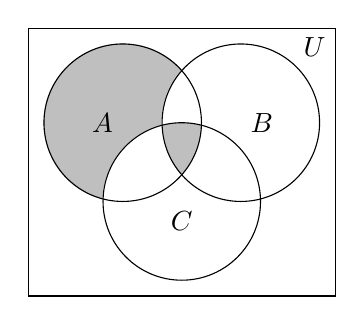
\begin{tikzpicture}
        \filldraw [gray!50] (0,0) circle (1);
        \filldraw [white] (1.5,0) circle (1);
        \filldraw [white] (0.75,-1) circle (1);
        \begin{scope}
            \clip (0,0) circle (1);
            \clip (1.5,0) circle (1);
            \clip (0.75,-1) circle (1);
            \filldraw [gray!50] (1.5,0) circle (1);
        \end{scope}
        \draw (0,0) circle (1) node [left] {$A$};
        \draw (1.5,0) circle (1) node [right] {$B$};
        \draw (0.75,-1) circle (1) node [below] {$C$};
        \draw (-1.2,-2.2) rectangle (2.7,1.2) node [below left] {$U$};
    \end{tikzpicture}
    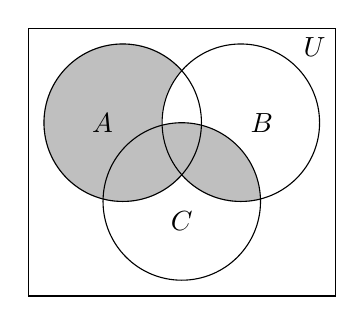
\begin{tikzpicture}
        \filldraw [gray!50] (0,0) circle (1);
        \filldraw [white] (1.5,0) circle (1);
        \begin{scope}
            \clip (0.75,-1) circle (1);
            \filldraw [gray!50] (1.5,0) circle (1);
        \end{scope}
        \draw (0,0) circle (1) node [left] {$A$};
        \draw (1.5,0) circle (1) node [right] {$B$};
        \draw (0.75,-1) circle (1) node [below] {$C$};
        \draw (-1.2,-2.2) rectangle (2.7,1.2) node [below left] {$U$};
    \end{tikzpicture}
\end{center}


关联目标:

暂未关联目标



标签: 第一单元

答案: 暂无答案

解答或提示: 暂无解答与提示

使用记录:

暂无使用记录


出处: 2025届高一校本作业必修第一章
\item { (020070)}判断下列语句是否为命题, 并在相应的横线上填入``是''或``否''.\\
(1) 正方形和四边形;\blank{50};\\
(2) 正方形是四边形吗?\blank{50};\\
(3) $\pi>3$;\blank{50};\\
(4) 正方形好美!\blank{50};\\
(5) $2x>4$;\blank{50};\\
(6) $968$能被$11$整除;\blank{50}.


关联目标:

暂未关联目标



标签: 第一单元

答案: 暂无答案

解答或提示: 暂无解答与提示

使用记录:

暂无使用记录


出处: 2025届高一校本作业必修第一章
\item { (020071)}判断下列命题的真假, 并在相应的括号内填入``真''或``假''.\\
(1) $2\sqrt 3>3\sqrt 2$或$1\le 1$;\blank{50};\\
(2) $2\sqrt 3>3\sqrt 2$且$1\le1$;\blank{50};\\
(3) 如果$a$、$b$都是奇数, 那么$ab$也是奇数;\blank{50};\\
(4) $\{1\}$是$\{0, 1, 2\}$的真子集;\blank{50};\\
(5) $1$是$\{0, 1, 2\}$的真子集;\blank{50};\\
(6) 若$x<-2$或$x>2$, 则$x^2>1$;\blank{50};\\
(7) 如果$|a|<2$, 那么$a<2$;\blank{50};\\
(8) 对任意实数$a,b$, 方程$(a+1)x+b=0$的解为$x=-\dfrac b{a+1}$;\blank{50};\\
(9) 若命题$\alpha$、$\beta$、$\gamma$满足$\alpha\Rightarrow \beta$, $\beta\Rightarrow \gamma$, $\gamma\Rightarrow \alpha$, 则$\alpha\Leftrightarrow \gamma$;\blank{50};\\
(10) 若关于$x$的方程$ax^2+bx+c=0$($a\ne 0$)的两实数根之积是正数, 则$ac>0$;\blank{50};\\
(11) 若某个整数不是偶数, 则这个数不能被$4$整除;\blank{50};\\
(12) 合数一定是偶数;\blank{50};\\
(13) 所有的偶数都是素数或合数;\blank{50};\\
(14) 所有的偶数都是素数或所有的偶数都是合数;\blank{50};\\
(15) 如果$A\subset B$, $B\supset C$, 那么$A=C$;\blank{50};\\
(16) 空集是任何集合的真子集;\blank{50};\\
(17) 若$x\in \mathbf{R}$, 则方程$x^2-x+1=0$不成立;\blank{50};\\
(18) 若$A\cap B\ne \varnothing$, $B\subset C$, 则$A\cap C\ne \varnothing$;\blank{50};\\
(19) 存在一个三角形, 它的任意两边的平方和小于第三边的平方;\blank{50};\\
(20) 对于任意一个三角形, 存在一组两边的平方和不等于第三边的平方;\blank{50}.


关联目标:

暂未关联目标



标签: 第一单元

答案: 暂无答案

解答或提示: 暂无解答与提示

使用记录:

暂无使用记录


出处: 2025届高一校本作业必修第一章
\item { (020073)}已知命题``非空集合$M$的元素都是集合$P$的元素$''$是假命题, 给出下列命题: \textcircled{1} $M$中的元素都不是$P$的元素; \textcircled{2} $M$中有不属于$P$的元素; \textcircled{3} $M$中有$P$的元素; \textcircled{4} $M$中的元素不都是$P$的元素. 其中真命题有\blank{50}.


关联目标:

暂未关联目标



标签: 第一单元

答案: 暂无答案

解答或提示: 暂无解答与提示

使用记录:

暂无使用记录


出处: 2025届高一校本作业必修第一章
\item { (020074)}已知$\alpha: 2\le x<4$, $\beta: 3m-1\le x\le-m$, 且$\alpha\Rightarrow\beta$, 求实数$m$的取值范围.


关联目标:

暂未关联目标



标签: 第一单元

答案: 暂无答案

解答或提示: 暂无解答与提示

使用记录:

暂无使用记录


出处: 2025届高一校本作业必修第一章
\item { (020075)}已知$a$是常数, 命题$\alpha :-1<a<3$, $\beta$: 关于$x$的方程$x+a=0$($x\in \mathbf{R}$)没有正根, 若命题$\alpha$、$\beta$有且只有一个是真命题, 求实数$a$的取值范围.


关联目标:

暂未关联目标



标签: 第一单元

答案: 暂无答案

解答或提示: 暂无解答与提示

使用记录:

暂无使用记录


出处: 2025届高一校本作业必修第一章
\item { (020076)}下列各题中$P$是$Q$的什么条件?(充分非必要、必要非充分、充要、既非充分又非必要)\\
(1) $P$: $x$是$2$的倍数, $Q$: $x$是$6$的倍数;\blank{50};\\
(2) $P$: $x$不是$2$的倍数, $Q$: $x$不是$6$的倍数;\blank{50};\\
(3) $P$: $x\in A$或$x\in B$, $Q$: $x\in A\cap B$;\blank{50};\\
(4) $P$: $f(x)=ax^2+bx+c$的图像过原点, $Q$: $c=0$;\blank{50}.


关联目标:

暂未关联目标



标签: 第一单元

答案: 暂无答案

解答或提示: 暂无解答与提示

使用记录:

暂无使用记录


出处: 2025届高一校本作业必修第一章
\item { (020077)}如果$A$是$B$的必要条件, $C$是$B$的充分条件, $A$是$C$的充分条件, 那么$B$、$C$分别是$A$的\blank{50}和\blank{50}条件.


关联目标:

暂未关联目标



标签: 第一单元

答案: 暂无答案

解答或提示: 暂无解答与提示

使用记录:

暂无使用记录


出处: 2025届高一校本作业必修第一章
\item { (020078)}写出使得``$x>3$''成立的一个充分条件: \blank{50}和一个必要条件: \blank{50}.


关联目标:

暂未关联目标



标签: 第一单元

答案: 暂无答案

解答或提示: 暂无解答与提示

使用记录:

暂无使用记录


出处: 2025届高一校本作业必修第一章
\item { (020080)}关于$x$的方程$ax^2=0$至少有一个实数根的一个充要条件是\blank{50}.


关联目标:

暂未关联目标



标签: 第一单元

答案: 暂无答案

解答或提示: 暂无解答与提示

使用记录:

暂无使用记录


出处: 2025届高一校本作业必修第一章
\item { (020082)}三个数$a$、$b$、$c$不全为零的充要条件是\bracket{20}.
\twoch{$a,b,c$都不是零}{$a,b,c$中最多一个零}{$a,b,c$中只有一个是零}{$a,b,c$中至少有一个不是零}


关联目标:

暂未关联目标



标签: 第一单元

答案: 暂无答案

解答或提示: 暂无解答与提示

使用记录:

暂无使用记录


出处: 2025届高一校本作业必修第一章
\item { (020083)}证明: $x_1>2$且$x_2>2$是$x_1+x_2>4$且$x_1\cdot x_2>4$的充分非必要条件.


关联目标:

暂未关联目标



标签: 第一单元

答案: 暂无答案

解答或提示: 暂无解答与提示

使用记录:

暂无使用记录


出处: 2025届高一校本作业必修第一章
\item { (020084)}有限集合$S$中元素的个数记作$\mathrm{card}(S)$, 设$A,B$都是有限集合, 给出下列命题:\\
\textcircled{1} $A\cap B=\varnothing$的一个充要条件是$\mathrm{card}(A\cup B)=\mathrm{card}(A)+\mathrm{card}(B)$;\\
\textcircled{2} $A\subseteq B$的一个必要不充分条件是$\mathrm{card}(A)\le \mathrm{card}(B)$; \\
\textcircled{3} $A$不是$B$的子集的一个充分不必要条件是$\mathrm{card}(A)>\mathrm{card}(B)$;\\ 
\textcircled{4} $A=B$的一个充要条件是$\mathrm{card}(A)=\mathrm{card}(B)$.\\ 
其中真命题的个数是\bracket{20}.
\fourch{$0$}{$1$}{$2$}{$3$}


关联目标:

暂未关联目标



标签: 第一单元

答案: 暂无答案

解答或提示: 暂无解答与提示

使用记录:

暂无使用记录


出处: 2025届高一校本作业必修第一章
\item { (020085)}设$\alpha,\beta$是方程$x^2-ax+b=0$的两个实数根. 试分析$a>2$且$b>1$是``两个实数根$\alpha,\beta$均大于$1$''的什么条件? 并证明你的结论.


关联目标:

暂未关联目标



标签: 第一单元

答案: 暂无答案

解答或提示: 暂无解答与提示

使用记录:

暂无使用记录


出处: 2025届高一校本作业必修第一章
\item { (020086)}设$x,y\in \mathbf{R}$, 求证: $|x+y|=|x|+|y|$成立的充要条件是$xy\ge 0$.


关联目标:

暂未关联目标



标签: 第一单元

答案: 暂无答案

解答或提示: 暂无解答与提示

使用记录:

暂无使用记录


出处: 2025届高一校本作业必修第一章
\item { (020087)}已知下列字母均为常实数, 写出下列陈述句的否定形式;
(1) $x>0$; \blank{100};\\
(2) $1>x>0$; \blank{100};\\
(3) $x>0$且$y\le 1$; \blank{100};\\
(4) $x>0$或$x\le -2$; \blank{100};\\
(5) $x\ne y$或$y\ne z$; \blank{100};\\
(6) $a,b,c,d$中至多有$2$个$0$; \blank{100};\\
(7) $a,b,c,d$中至少有$2$个$1$; \blank{100};\\
(8) $a,b,c,d$都大于$1$; \blank{100};\\
(9) $a,b,c,d$不都大于$1$; \blank{100};\\
(10) $a,b,c,d$都不大于$1$; \blank{100}.


关联目标:

暂未关联目标



标签: 第一单元

答案: 暂无答案

解答或提示: 暂无解答与提示

使用记录:

暂无使用记录


出处: 2025届高一校本作业必修第一章
\item { (020088)}在横线上写出下列命题的否定形式, 并判断命题真假, 在相应的位置中填入``真''或``假''.\\
(1) $\pi$是无理数; \blank{20}; \blank{150}; \blank{20};\\
(2) $2+1=4$;  \blank{20}; \blank{150}; \blank{20};\\
(3) 任何实数是正数或负数;  \blank{20}; \blank{150}; \blank{20};\\
(4) 任何实数是正数或任何实数是负数;  \blank{20}; \blank{150}; \blank{20};\\
(5) 对一切实数$x, x^3+1=0$;  \blank{20}; \blank{150}; \blank{20};\\
(6) 存在实数$x, x^3+1=0$;  \blank{20}; \blank{150}; \blank{20};\\
(7) 对于任意实数$k$, 关于$x$的方程$x^2+x+k=0$都有实数根;  \blank{20}; \blank{250}; \blank{20};\\
(8) 任何三角形中至多有一个钝角;  \blank{20}; \blank{150}; \blank{20};\\
(9) 若$a>1$, $b>1$, 则$ab>1$;  \blank{20}; \blank{150}; \blank{20};\\
(10) 能被$2$整除的整数是质数;  \blank{20}; \blank{150}; \blank{20}.\\


关联目标:

暂未关联目标



标签: 第一单元

答案: 暂无答案

解答或提示: 暂无解答与提示

使用记录:

暂无使用记录


出处: 2025届高一校本作业必修第一章
\item { (020090)}已知甲$\Rightarrow$乙, 下列说法一定正确的是\bracket{20}.
\twoch{甲不成立, 可推出乙成立}{甲不成立, 可推出乙不成立}{乙不成立, 可推出甲成立}{乙不成立, 可推出甲不成立}


关联目标:

暂未关联目标



标签: 第一单元

答案: 暂无答案

解答或提示: 暂无解答与提示

使用记录:

暂无使用记录


出处: 2025届高一校本作业必修第一章
\item { (020091)}``$a\ne 1$且$b\ne 2$''是``$a+b\ne 3$''的\bracket{20}.
\twoch{充分非必要条件}{必要非充分条件}{充要条件}{既非充分又非必要条件}


关联目标:

暂未关联目标



标签: 第一单元

答案: 暂无答案

解答或提示: 暂无解答与提示

使用记录:

暂无使用记录


出处: 2025届高一校本作业必修第一章
\item { (020092)}证明: 若$x+2y+z>0$, 则$x,y,z$中至少有一个大于$0$.


关联目标:

暂未关联目标



标签: 第一单元

答案: 暂无答案

解答或提示: 暂无解答与提示

使用记录:

暂无使用记录


出处: 2025届高一校本作业必修第一章
\item { (020093)}证明:对于三个实数$a,b,c$, 若$a\ne c$, 则$a\ne b$或$b\ne c$.


关联目标:

暂未关联目标



标签: 第一单元

答案: 暂无答案

解答或提示: 暂无解答与提示

使用记录:

暂无使用记录


出处: 2025届高一校本作业必修第一章
\item { (020094)}``$x\ne 3$或$x\ne 4$'' 是``$x^2-7x+12\ne 0$''的\bracket{20}.
\twoch{充分非必要条件}{必要非充分条件}{充要条件}{既非充分又非必要条件}


关联目标:

暂未关联目标



标签: 第一单元

答案: 暂无答案

解答或提示: 暂无解答与提示

使用记录:

暂无使用记录


出处: 2025届高一校本作业必修第一章
\item { (020095)}证明: 若$x^2\ne y^2$, 则$x\ne y$或$x\ne -y$.


关联目标:

暂未关联目标



标签: 第一单元

答案: 暂无答案

解答或提示: 暂无解答与提示

使用记录:

暂无使用记录


出处: 2025届高一校本作业必修第一章
\item { (020096)}若$a^3+b^3=2$, 证明: $a+b\le 2$.


关联目标:

暂未关联目标



标签: 第一单元

答案: 暂无答案

解答或提示: 暂无解答与提示

使用记录:

暂无使用记录


出处: 2025届高一校本作业必修第一章
\end{enumerate}



\end{document}